\documentclass[twoside]{book}

% Packages required by doxygen
\usepackage{fixltx2e}
\usepackage{calc}
\usepackage{doxygen}
\usepackage[export]{adjustbox} % also loads graphicx
\usepackage{graphicx}
\usepackage[utf8]{inputenc}
\usepackage{makeidx}
\usepackage{multicol}
\usepackage{multirow}
\PassOptionsToPackage{warn}{textcomp}
\usepackage{textcomp}
\usepackage[nointegrals]{wasysym}
\usepackage[table]{xcolor}

% Font selection
\usepackage[T1]{fontenc}
\usepackage[scaled=.90]{helvet}
\usepackage{courier}
\usepackage{amssymb}
\usepackage{sectsty}
\renewcommand{\familydefault}{\sfdefault}
\allsectionsfont{%
  \fontseries{bc}\selectfont%
  \color{darkgray}%
}
\renewcommand{\DoxyLabelFont}{%
  \fontseries{bc}\selectfont%
  \color{darkgray}%
}
\newcommand{\+}{\discretionary{\mbox{\scriptsize$\hookleftarrow$}}{}{}}

% Page & text layout
\usepackage{geometry}
\geometry{%
  a4paper,%
  top=2.5cm,%
  bottom=2.5cm,%
  left=2.5cm,%
  right=2.5cm%
}
\tolerance=750
\hfuzz=15pt
\hbadness=750
\setlength{\emergencystretch}{15pt}
\setlength{\parindent}{0cm}
\setlength{\parskip}{3ex plus 2ex minus 2ex}
\makeatletter
\renewcommand{\paragraph}{%
  \@startsection{paragraph}{4}{0ex}{-1.0ex}{1.0ex}{%
    \normalfont\normalsize\bfseries\SS@parafont%
  }%
}
\renewcommand{\subparagraph}{%
  \@startsection{subparagraph}{5}{0ex}{-1.0ex}{1.0ex}{%
    \normalfont\normalsize\bfseries\SS@subparafont%
  }%
}
\makeatother

% Headers & footers
\usepackage{fancyhdr}
\pagestyle{fancyplain}
\fancyhead[LE]{\fancyplain{}{\bfseries\thepage}}
\fancyhead[CE]{\fancyplain{}{}}
\fancyhead[RE]{\fancyplain{}{\bfseries\leftmark}}
\fancyhead[LO]{\fancyplain{}{\bfseries\rightmark}}
\fancyhead[CO]{\fancyplain{}{}}
\fancyhead[RO]{\fancyplain{}{\bfseries\thepage}}
\fancyfoot[LE]{\fancyplain{}{}}
\fancyfoot[CE]{\fancyplain{}{}}
\fancyfoot[RE]{\fancyplain{}{\bfseries\scriptsize Generated by Doxygen }}
\fancyfoot[LO]{\fancyplain{}{\bfseries\scriptsize Generated by Doxygen }}
\fancyfoot[CO]{\fancyplain{}{}}
\fancyfoot[RO]{\fancyplain{}{}}
\renewcommand{\footrulewidth}{0.4pt}
\renewcommand{\chaptermark}[1]{%
  \markboth{#1}{}%
}
\renewcommand{\sectionmark}[1]{%
  \markright{\thesection\ #1}%
}

% Indices & bibliography
\usepackage{natbib}
\usepackage[titles]{tocloft}
\setcounter{tocdepth}{3}
\setcounter{secnumdepth}{5}
\makeindex

% Hyperlinks (required, but should be loaded last)
\usepackage{ifpdf}
\ifpdf
  \usepackage[pdftex,pagebackref=true]{hyperref}
\else
  \usepackage[ps2pdf,pagebackref=true]{hyperref}
\fi
\hypersetup{%
  colorlinks=true,%
  linkcolor=blue,%
  citecolor=blue,%
  unicode%
}

% Custom commands
\newcommand{\clearemptydoublepage}{%
  \newpage{\pagestyle{empty}\cleardoublepage}%
}

\usepackage{caption}
\captionsetup{labelsep=space,justification=centering,font={bf},singlelinecheck=off,skip=4pt,position=top}

%===== C O N T E N T S =====

\begin{document}

% Titlepage & ToC
\hypersetup{pageanchor=false,
             bookmarksnumbered=true,
             pdfencoding=unicode
            }
\pagenumbering{alph}
\begin{titlepage}
\vspace*{7cm}
\begin{center}%
{\Large Code\+Control \\[1ex]\large Version 1.\+0 -\/-\/ June 2017 }\\
\vspace*{1cm}
{\large Generated by Doxygen 1.8.13}\\
\end{center}
\end{titlepage}
\clearemptydoublepage
\pagenumbering{roman}
\tableofcontents
\clearemptydoublepage
\pagenumbering{arabic}
\hypersetup{pageanchor=true}

%--- Begin generated contents ---
\chapter{Hierarchical Index}
\section{Class Hierarchy}
This inheritance list is sorted roughly, but not completely, alphabetically\+:\begin{DoxyCompactList}
\item Asset\+Postprocessor\begin{DoxyCompactList}
\item \contentsline{section}{Analytics\+Dependencies}{\pageref{class_analytics_dependencies}}{}
\end{DoxyCompactList}
\item \contentsline{section}{Field}{\pageref{class_field}}{}
\item \contentsline{section}{Fields}{\pageref{class_fields}}{}
\item \contentsline{section}{Google\+Analyticsi\+O\+S\+V3}{\pageref{class_google_analyticsi_o_s_v3}}{}
\item \contentsline{section}{Google\+Analytics\+M\+P\+V3}{\pageref{class_google_analytics_m_p_v3}}{}
\item \contentsline{section}{Hit\+Builder$<$ T $>$}{\pageref{class_hit_builder}}{}
\item \contentsline{section}{Hit\+Builder$<$ App\+View\+Hit\+Builder $>$}{\pageref{class_hit_builder}}{}
\begin{DoxyCompactList}
\item \contentsline{section}{App\+View\+Hit\+Builder}{\pageref{class_app_view_hit_builder}}{}
\end{DoxyCompactList}
\item \contentsline{section}{Hit\+Builder$<$ Event\+Hit\+Builder $>$}{\pageref{class_hit_builder}}{}
\begin{DoxyCompactList}
\item \contentsline{section}{Event\+Hit\+Builder}{\pageref{class_event_hit_builder}}{}
\end{DoxyCompactList}
\item \contentsline{section}{Hit\+Builder$<$ Exception\+Hit\+Builder $>$}{\pageref{class_hit_builder}}{}
\begin{DoxyCompactList}
\item \contentsline{section}{Exception\+Hit\+Builder}{\pageref{class_exception_hit_builder}}{}
\end{DoxyCompactList}
\item \contentsline{section}{Hit\+Builder$<$ Item\+Hit\+Builder $>$}{\pageref{class_hit_builder}}{}
\begin{DoxyCompactList}
\item \contentsline{section}{Item\+Hit\+Builder}{\pageref{class_item_hit_builder}}{}
\end{DoxyCompactList}
\item \contentsline{section}{Hit\+Builder$<$ Social\+Hit\+Builder $>$}{\pageref{class_hit_builder}}{}
\begin{DoxyCompactList}
\item \contentsline{section}{Social\+Hit\+Builder}{\pageref{class_social_hit_builder}}{}
\end{DoxyCompactList}
\item \contentsline{section}{Hit\+Builder$<$ Timing\+Hit\+Builder $>$}{\pageref{class_hit_builder}}{}
\begin{DoxyCompactList}
\item \contentsline{section}{Timing\+Hit\+Builder}{\pageref{class_timing_hit_builder}}{}
\end{DoxyCompactList}
\item \contentsline{section}{Hit\+Builder$<$ Transaction\+Hit\+Builder $>$}{\pageref{class_hit_builder}}{}
\begin{DoxyCompactList}
\item \contentsline{section}{Transaction\+Hit\+Builder}{\pageref{class_transaction_hit_builder}}{}
\end{DoxyCompactList}
\item I\+Disposable\begin{DoxyCompactList}
\item \contentsline{section}{Google\+Analytics\+Android\+V4}{\pageref{class_google_analytics_android_v4}}{}
\end{DoxyCompactList}
\item Mono\+Behaviour\begin{DoxyCompactList}
\item \contentsline{section}{Analytics\+By\+Level}{\pageref{class_analytics_by_level}}{}
\item \contentsline{section}{Arith\+Completion\+Check}{\pageref{class_arith_completion_check}}{}
\item \contentsline{section}{arithmetic\+Teleporter}{\pageref{classarithmetic_teleporter}}{}
\item \contentsline{section}{Array\+Access\+Completion}{\pageref{class_array_access_completion}}{}
\item \contentsline{section}{Array\+Box\+Controller}{\pageref{class_array_box_controller}}{}
\item \contentsline{section}{Array\+Reaction}{\pageref{class_array_reaction}}{}
\item \contentsline{section}{Array\+Sum\+Completion}{\pageref{class_array_sum_completion}}{}
\item \contentsline{section}{Array\+Teleporter}{\pageref{class_array_teleporter}}{}
\item \contentsline{section}{Array\+Tile\+Controller}{\pageref{class_array_tile_controller}}{}
\item \contentsline{section}{Arr\+Cams\+Controller}{\pageref{class_arr_cams_controller}}{}
\item \contentsline{section}{bomb\+Logic}{\pageref{classbomb_logic}}{}
\item \contentsline{section}{Bool\+Ops\+Completion}{\pageref{class_bool_ops_completion}}{}
\item \contentsline{section}{Camera\+Follow}{\pageref{class_camera_follow}}{}
\item \contentsline{section}{camera\+Zoom}{\pageref{classcamera_zoom}}{}
\item \contentsline{section}{Completion\+Check}{\pageref{class_completion_check}}{}
\item \contentsline{section}{Completion\+Check2}{\pageref{class_completion_check2}}{}
\item \contentsline{section}{Completion\+Script\+Four}{\pageref{class_completion_script_four}}{}
\item \contentsline{section}{Completion\+Script\+Three}{\pageref{class_completion_script_three}}{}
\item \contentsline{section}{Console}{\pageref{class_console}}{}
\item \contentsline{section}{Credits\+Script}{\pageref{class_credits_script}}{}
\item \contentsline{section}{Data\+Type\+Completion\+Check}{\pageref{class_data_type_completion_check}}{}
\item \contentsline{section}{Desktop\+Controller}{\pageref{class_desktop_controller}}{}
\item \contentsline{section}{Desktop\+Controller\+Box\+Array}{\pageref{class_desktop_controller_box_array}}{}
\item \contentsline{section}{Desktop\+Interaction}{\pageref{class_desktop_interaction}}{}
\item \contentsline{section}{Elevator\+Controller}{\pageref{class_elevator_controller}}{}
\item \contentsline{section}{E\+S\+C\+P\+O\+D\+\_\+\+Control}{\pageref{class_e_s_c_p_o_d___control}}{}
\item \contentsline{section}{E\+S\+C\+P\+O\+D\+\_\+\+Control2}{\pageref{class_e_s_c_p_o_d___control2}}{}
\item \contentsline{section}{Exit\+Door\+Logic\+Conditionals}{\pageref{class_exit_door_logic_conditionals}}{}
\item \contentsline{section}{explode\+Logic}{\pageref{classexplode_logic}}{}
\item \contentsline{section}{Final\+Puzzle\+Completion\+Check}{\pageref{class_final_puzzle_completion_check}}{}
\item \contentsline{section}{Final\+Room\+Door}{\pageref{class_final_room_door}}{}
\item \contentsline{section}{For\+Loop\+Desk\+Top\+Interaction}{\pageref{class_for_loop_desk_top_interaction}}{}
\item \contentsline{section}{Game\+Buttons}{\pageref{class_game_buttons}}{}
\item \contentsline{section}{Global\+Controller}{\pageref{class_global_controller}}{}
\item \contentsline{section}{Google\+Analytics\+V4}{\pageref{class_google_analytics_v4}}{}
\item \contentsline{section}{Help\+Buttons}{\pageref{class_help_buttons}}{}
\item \contentsline{section}{Indent\+Puzzle}{\pageref{class_indent_puzzle}}{}
\item \contentsline{section}{Insert\+Puzzle\+Completion}{\pageref{class_insert_puzzle_completion}}{}
\item \contentsline{section}{Intro\+Level\+Manager}{\pageref{class_intro_level_manager}}{}
\item \contentsline{section}{J\+I\+T\+Level1}{\pageref{class_j_i_t_level1}}{}
\item \contentsline{section}{J\+I\+T\+Script}{\pageref{class_j_i_t_script}}{}
\item \contentsline{section}{laser\+Sound\+Script}{\pageref{classlaser_sound_script}}{}
\item \contentsline{section}{Left\+Laser\+Interaction}{\pageref{class_left_laser_interaction}}{}
\item \contentsline{section}{level\+Complete\+Arith}{\pageref{classlevel_complete_arith}}{}
\item \contentsline{section}{level\+Complete\+Array}{\pageref{classlevel_complete_array}}{}
\item \contentsline{section}{level\+Complete\+Cond}{\pageref{classlevel_complete_cond}}{}
\item \contentsline{section}{level\+Complete\+Loop}{\pageref{classlevel_complete_loop}}{}
\item \contentsline{section}{Logical\+And\+Completion}{\pageref{class_logical_and_completion}}{}
\item \contentsline{section}{Logical\+Or\+Completion}{\pageref{class_logical_or_completion}}{}
\item \contentsline{section}{Loop\+Teleporter}{\pageref{class_loop_teleporter}}{}
\item \contentsline{section}{Message\+Panel}{\pageref{class_message_panel}}{}
\item \contentsline{section}{Moving\+Object}{\pageref{class_moving_object}}{}
\item \contentsline{section}{Nested\+For\+Desk\+Top\+Interaction}{\pageref{class_nested_for_desk_top_interaction}}{}
\item \contentsline{section}{Nested\+For\+J\+IT}{\pageref{class_nested_for_j_i_t}}{}
\item \contentsline{section}{One\+Way\+Moving\+Object}{\pageref{class_one_way_moving_object}}{}
\item \contentsline{section}{One\+Way\+Moving\+Object\+Trigger}{\pageref{class_one_way_moving_object_trigger}}{}
\item \contentsline{section}{P2}{\pageref{class_p2}}{}
\item \contentsline{section}{Pause\+Menu}{\pageref{class_pause_menu}}{}
\item \contentsline{section}{place\+Scientists}{\pageref{classplace_scientists}}{}
\item \contentsline{section}{Platform\+Access\+Controller}{\pageref{class_platform_access_controller}}{}
\item \contentsline{section}{Player\+Movement}{\pageref{class_player_movement}}{}
\item \contentsline{section}{react\+To\+Break\+One}{\pageref{classreact_to_break_one}}{}
\item \contentsline{section}{react\+To\+Break\+Three}{\pageref{classreact_to_break_three}}{}
\item \contentsline{section}{react\+To\+Break\+Two}{\pageref{classreact_to_break_two}}{}
\item \contentsline{section}{react\+To\+Int}{\pageref{classreact_to_int}}{}
\item \contentsline{section}{React\+To\+Plus\+P4}{\pageref{class_react_to_plus_p4}}{}
\item \contentsline{section}{React\+To\+Plus\+Plus\+P4}{\pageref{class_react_to_plus_plus_p4}}{}
\item \contentsline{section}{react\+To\+Switch\+Condition}{\pageref{classreact_to_switch_condition}}{}
\item \contentsline{section}{React\+To\+Tile}{\pageref{class_react_to_tile}}{}
\item \contentsline{section}{React\+To\+Tile\+Five}{\pageref{class_react_to_tile_five}}{}
\item \contentsline{section}{React\+To\+Tile\+Plus}{\pageref{class_react_to_tile_plus}}{}
\item \contentsline{section}{React\+To\+Tile\+Plus\+L2}{\pageref{class_react_to_tile_plus_l2}}{}
\item \contentsline{section}{React\+To\+Tile\+Plus\+Plus}{\pageref{class_react_to_tile_plus_plus}}{}
\item \contentsline{section}{React\+To\+Tile\+Plus\+Plus\+L2}{\pageref{class_react_to_tile_plus_plus_l2}}{}
\item \contentsline{section}{React\+To\+Tile\+Three}{\pageref{class_react_to_tile_three}}{}
\item \contentsline{section}{React\+To\+TileX}{\pageref{class_react_to_tile_x}}{}
\item \contentsline{section}{React\+To\+TileY}{\pageref{class_react_to_tile_y}}{}
\item \contentsline{section}{Reactto\+X\+P4}{\pageref{class_reactto_x_p4}}{}
\item \contentsline{section}{reset\+Button}{\pageref{classreset_button}}{}
\item \contentsline{section}{Respawn\+Controller}{\pageref{class_respawn_controller}}{}
\item \contentsline{section}{Return\+To\+Home\+Portal}{\pageref{class_return_to_home_portal}}{}
\item \contentsline{section}{Rising\+Platform\+Controller}{\pageref{class_rising_platform_controller}}{}
\item \contentsline{section}{scientist\+Run}{\pageref{classscientist_run}}{}
\item \contentsline{section}{secret\+Door}{\pageref{classsecret_door}}{}
\item \contentsline{section}{Settings\+Script}{\pageref{class_settings_script}}{}
\item \contentsline{section}{Single\+For\+J\+IT}{\pageref{class_single_for_j_i_t}}{}
\item \contentsline{section}{submit\+Button}{\pageref{classsubmit_button}}{}
\item \contentsline{section}{Switch\+Console\+Behaviour}{\pageref{class_switch_console_behaviour}}{}
\item \contentsline{section}{Teleporter\+Controller}{\pageref{class_teleporter_controller}}{}
\item \contentsline{section}{Tile\+Drag}{\pageref{class_tile_drag}}{}
\item \contentsline{section}{Title\+Screen\+Controller}{\pageref{class_title_screen_controller}}{}
\item \contentsline{section}{While\+J\+IT}{\pageref{class_while_j_i_t}}{}
\item \contentsline{section}{While\+Loop\+Desktop\+Interaction}{\pageref{class_while_loop_desktop_interaction}}{}
\end{DoxyCompactList}
\item N\+S\+Object\begin{DoxyCompactList}
\item \contentsline{section}{G\+AI}{\pageref{interface_g_a_i}}{}
\item \contentsline{section}{G\+A\+I\+Dictionary\+Builder}{\pageref{interface_g_a_i_dictionary_builder}}{}
\item \contentsline{section}{G\+A\+I\+Ecommerce\+Fields}{\pageref{interface_g_a_i_ecommerce_fields}}{}
\item \contentsline{section}{G\+A\+I\+Ecommerce\+Product}{\pageref{interface_g_a_i_ecommerce_product}}{}
\item \contentsline{section}{G\+A\+I\+Ecommerce\+Product\+Action}{\pageref{interface_g_a_i_ecommerce_product_action}}{}
\item \contentsline{section}{G\+A\+I\+Ecommerce\+Promotion}{\pageref{interface_g_a_i_ecommerce_promotion}}{}
\item \contentsline{section}{G\+A\+I\+Fields}{\pageref{interface_g_a_i_fields}}{}
\item \contentsline{section}{G\+A\+I\+Handler}{\pageref{class_g_a_i_handler}}{}
\end{DoxyCompactList}
\item $<$N\+S\+Object$>$\begin{DoxyCompactList}
\item \contentsline{section}{$<$G\+A\+I\+Logger$>$}{\pageref{protocol_g_a_i_logger-p}}{}
\item \contentsline{section}{$<$G\+A\+I\+Tracker$>$}{\pageref{protocol_g_a_i_tracker-p}}{}
\end{DoxyCompactList}
\item Property\+Attribute\begin{DoxyCompactList}
\item \contentsline{section}{Advertiser\+Opt\+In\+Attribute}{\pageref{class_advertiser_opt_in_attribute}}{}
\item \contentsline{section}{Ranged\+Tooltip\+Attribute}{\pageref{class_ranged_tooltip_attribute}}{}
\item \contentsline{section}{Tooltip\+Attribute}{\pageref{class_tooltip_attribute}}{}
\end{DoxyCompactList}
\item Property\+Drawer\begin{DoxyCompactList}
\item \contentsline{section}{Tooltip\+Drawer}{\pageref{class_tooltip_drawer}}{}
\end{DoxyCompactList}
\item U\+I\+View\+Controller\begin{DoxyCompactList}
\item \contentsline{section}{G\+A\+I\+Tracked\+View\+Controller}{\pageref{interface_g_a_i_tracked_view_controller}}{}
\end{DoxyCompactList}
\end{DoxyCompactList}

\chapter{Class Index}
\section{Class List}
Here are the classes, structs, unions and interfaces with brief descriptions\+:\begin{DoxyCompactList}
\item\contentsline{section}{\hyperlink{class_advertiser_opt_in_attribute}{Advertiser\+Opt\+In\+Attribute} }{\pageref{class_advertiser_opt_in_attribute}}{}
\item\contentsline{section}{\hyperlink{class_analytics_by_level}{Analytics\+By\+Level} }{\pageref{class_analytics_by_level}}{}
\item\contentsline{section}{\hyperlink{class_analytics_dependencies}{Analytics\+Dependencies} }{\pageref{class_analytics_dependencies}}{}
\item\contentsline{section}{\hyperlink{class_app_view_hit_builder}{App\+View\+Hit\+Builder} }{\pageref{class_app_view_hit_builder}}{}
\item\contentsline{section}{\hyperlink{class_arith_completion_check}{Arith\+Completion\+Check} }{\pageref{class_arith_completion_check}}{}
\item\contentsline{section}{\hyperlink{classarithmetic_teleporter}{arithmetic\+Teleporter} }{\pageref{classarithmetic_teleporter}}{}
\item\contentsline{section}{\hyperlink{class_array_access_completion}{Array\+Access\+Completion} }{\pageref{class_array_access_completion}}{}
\item\contentsline{section}{\hyperlink{class_array_box_controller}{Array\+Box\+Controller} }{\pageref{class_array_box_controller}}{}
\item\contentsline{section}{\hyperlink{class_array_reaction}{Array\+Reaction} }{\pageref{class_array_reaction}}{}
\item\contentsline{section}{\hyperlink{class_array_sum_completion}{Array\+Sum\+Completion} }{\pageref{class_array_sum_completion}}{}
\item\contentsline{section}{\hyperlink{class_array_teleporter}{Array\+Teleporter} }{\pageref{class_array_teleporter}}{}
\item\contentsline{section}{\hyperlink{class_array_tile_controller}{Array\+Tile\+Controller} }{\pageref{class_array_tile_controller}}{}
\item\contentsline{section}{\hyperlink{class_arr_cams_controller}{Arr\+Cams\+Controller} }{\pageref{class_arr_cams_controller}}{}
\item\contentsline{section}{\hyperlink{classbomb_logic}{bomb\+Logic} }{\pageref{classbomb_logic}}{}
\item\contentsline{section}{\hyperlink{class_bool_ops_completion}{Bool\+Ops\+Completion} }{\pageref{class_bool_ops_completion}}{}
\item\contentsline{section}{\hyperlink{class_camera_follow}{Camera\+Follow} }{\pageref{class_camera_follow}}{}
\item\contentsline{section}{\hyperlink{classcamera_zoom}{camera\+Zoom} }{\pageref{classcamera_zoom}}{}
\item\contentsline{section}{\hyperlink{class_completion_check}{Completion\+Check} }{\pageref{class_completion_check}}{}
\item\contentsline{section}{\hyperlink{class_completion_check2}{Completion\+Check2} }{\pageref{class_completion_check2}}{}
\item\contentsline{section}{\hyperlink{class_completion_script_four}{Completion\+Script\+Four} }{\pageref{class_completion_script_four}}{}
\item\contentsline{section}{\hyperlink{class_completion_script_three}{Completion\+Script\+Three} }{\pageref{class_completion_script_three}}{}
\item\contentsline{section}{\hyperlink{class_console}{Console} }{\pageref{class_console}}{}
\item\contentsline{section}{\hyperlink{class_credits_script}{Credits\+Script} }{\pageref{class_credits_script}}{}
\item\contentsline{section}{\hyperlink{class_data_type_completion_check}{Data\+Type\+Completion\+Check} }{\pageref{class_data_type_completion_check}}{}
\item\contentsline{section}{\hyperlink{class_desktop_controller}{Desktop\+Controller} }{\pageref{class_desktop_controller}}{}
\item\contentsline{section}{\hyperlink{class_desktop_controller_box_array}{Desktop\+Controller\+Box\+Array} }{\pageref{class_desktop_controller_box_array}}{}
\item\contentsline{section}{\hyperlink{class_desktop_interaction}{Desktop\+Interaction} }{\pageref{class_desktop_interaction}}{}
\item\contentsline{section}{\hyperlink{class_elevator_controller}{Elevator\+Controller} }{\pageref{class_elevator_controller}}{}
\item\contentsline{section}{\hyperlink{class_e_s_c_p_o_d___control}{E\+S\+C\+P\+O\+D\+\_\+\+Control} }{\pageref{class_e_s_c_p_o_d___control}}{}
\item\contentsline{section}{\hyperlink{class_e_s_c_p_o_d___control2}{E\+S\+C\+P\+O\+D\+\_\+\+Control2} }{\pageref{class_e_s_c_p_o_d___control2}}{}
\item\contentsline{section}{\hyperlink{class_event_hit_builder}{Event\+Hit\+Builder} }{\pageref{class_event_hit_builder}}{}
\item\contentsline{section}{\hyperlink{class_exception_hit_builder}{Exception\+Hit\+Builder} }{\pageref{class_exception_hit_builder}}{}
\item\contentsline{section}{\hyperlink{class_exit_door_logic_conditionals}{Exit\+Door\+Logic\+Conditionals} }{\pageref{class_exit_door_logic_conditionals}}{}
\item\contentsline{section}{\hyperlink{classexplode_logic}{explode\+Logic} }{\pageref{classexplode_logic}}{}
\item\contentsline{section}{\hyperlink{class_field}{Field} }{\pageref{class_field}}{}
\item\contentsline{section}{\hyperlink{class_fields}{Fields} }{\pageref{class_fields}}{}
\item\contentsline{section}{\hyperlink{class_final_puzzle_completion_check}{Final\+Puzzle\+Completion\+Check} }{\pageref{class_final_puzzle_completion_check}}{}
\item\contentsline{section}{\hyperlink{class_final_room_door}{Final\+Room\+Door} }{\pageref{class_final_room_door}}{}
\item\contentsline{section}{\hyperlink{class_for_loop_desk_top_interaction}{For\+Loop\+Desk\+Top\+Interaction} }{\pageref{class_for_loop_desk_top_interaction}}{}
\item\contentsline{section}{\hyperlink{interface_g_a_i}{G\+AI} }{\pageref{interface_g_a_i}}{}
\item\contentsline{section}{\hyperlink{interface_g_a_i_dictionary_builder}{G\+A\+I\+Dictionary\+Builder} }{\pageref{interface_g_a_i_dictionary_builder}}{}
\item\contentsline{section}{\hyperlink{interface_g_a_i_ecommerce_fields}{G\+A\+I\+Ecommerce\+Fields} }{\pageref{interface_g_a_i_ecommerce_fields}}{}
\item\contentsline{section}{\hyperlink{interface_g_a_i_ecommerce_product}{G\+A\+I\+Ecommerce\+Product} }{\pageref{interface_g_a_i_ecommerce_product}}{}
\item\contentsline{section}{\hyperlink{interface_g_a_i_ecommerce_product_action}{G\+A\+I\+Ecommerce\+Product\+Action} }{\pageref{interface_g_a_i_ecommerce_product_action}}{}
\item\contentsline{section}{\hyperlink{interface_g_a_i_ecommerce_promotion}{G\+A\+I\+Ecommerce\+Promotion} }{\pageref{interface_g_a_i_ecommerce_promotion}}{}
\item\contentsline{section}{\hyperlink{interface_g_a_i_fields}{G\+A\+I\+Fields} }{\pageref{interface_g_a_i_fields}}{}
\item\contentsline{section}{\hyperlink{class_g_a_i_handler}{G\+A\+I\+Handler} }{\pageref{class_g_a_i_handler}}{}
\item\contentsline{section}{\hyperlink{protocol_g_a_i_logger-p}{$<$\+G\+A\+I\+Logger$>$} }{\pageref{protocol_g_a_i_logger-p}}{}
\item\contentsline{section}{\hyperlink{interface_g_a_i_tracked_view_controller}{G\+A\+I\+Tracked\+View\+Controller} }{\pageref{interface_g_a_i_tracked_view_controller}}{}
\item\contentsline{section}{\hyperlink{protocol_g_a_i_tracker-p}{$<$\+G\+A\+I\+Tracker$>$} }{\pageref{protocol_g_a_i_tracker-p}}{}
\item\contentsline{section}{\hyperlink{class_game_buttons}{Game\+Buttons} }{\pageref{class_game_buttons}}{}
\item\contentsline{section}{\hyperlink{class_global_controller}{Global\+Controller} }{\pageref{class_global_controller}}{}
\item\contentsline{section}{\hyperlink{class_google_analytics_android_v4}{Google\+Analytics\+Android\+V4} }{\pageref{class_google_analytics_android_v4}}{}
\item\contentsline{section}{\hyperlink{class_google_analyticsi_o_s_v3}{Google\+Analyticsi\+O\+S\+V3} }{\pageref{class_google_analyticsi_o_s_v3}}{}
\item\contentsline{section}{\hyperlink{class_google_analytics_m_p_v3}{Google\+Analytics\+M\+P\+V3} }{\pageref{class_google_analytics_m_p_v3}}{}
\item\contentsline{section}{\hyperlink{class_google_analytics_v4}{Google\+Analytics\+V4} }{\pageref{class_google_analytics_v4}}{}
\item\contentsline{section}{\hyperlink{class_help_buttons}{Help\+Buttons} }{\pageref{class_help_buttons}}{}
\item\contentsline{section}{\hyperlink{class_hit_builder}{Hit\+Builder$<$ T $>$} }{\pageref{class_hit_builder}}{}
\item\contentsline{section}{\hyperlink{class_indent_puzzle}{Indent\+Puzzle} }{\pageref{class_indent_puzzle}}{}
\item\contentsline{section}{\hyperlink{class_insert_puzzle_completion}{Insert\+Puzzle\+Completion} }{\pageref{class_insert_puzzle_completion}}{}
\item\contentsline{section}{\hyperlink{class_intro_level_manager}{Intro\+Level\+Manager} }{\pageref{class_intro_level_manager}}{}
\item\contentsline{section}{\hyperlink{class_item_hit_builder}{Item\+Hit\+Builder} }{\pageref{class_item_hit_builder}}{}
\item\contentsline{section}{\hyperlink{class_j_i_t_level1}{J\+I\+T\+Level1} }{\pageref{class_j_i_t_level1}}{}
\item\contentsline{section}{\hyperlink{class_j_i_t_script}{J\+I\+T\+Script} }{\pageref{class_j_i_t_script}}{}
\item\contentsline{section}{\hyperlink{classlaser_sound_script}{laser\+Sound\+Script} }{\pageref{classlaser_sound_script}}{}
\item\contentsline{section}{\hyperlink{class_left_laser_interaction}{Left\+Laser\+Interaction} }{\pageref{class_left_laser_interaction}}{}
\item\contentsline{section}{\hyperlink{classlevel_complete_arith}{level\+Complete\+Arith} }{\pageref{classlevel_complete_arith}}{}
\item\contentsline{section}{\hyperlink{classlevel_complete_array}{level\+Complete\+Array} }{\pageref{classlevel_complete_array}}{}
\item\contentsline{section}{\hyperlink{classlevel_complete_cond}{level\+Complete\+Cond} }{\pageref{classlevel_complete_cond}}{}
\item\contentsline{section}{\hyperlink{classlevel_complete_loop}{level\+Complete\+Loop} }{\pageref{classlevel_complete_loop}}{}
\item\contentsline{section}{\hyperlink{class_logical_and_completion}{Logical\+And\+Completion} }{\pageref{class_logical_and_completion}}{}
\item\contentsline{section}{\hyperlink{class_logical_or_completion}{Logical\+Or\+Completion} }{\pageref{class_logical_or_completion}}{}
\item\contentsline{section}{\hyperlink{class_loop_teleporter}{Loop\+Teleporter} }{\pageref{class_loop_teleporter}}{}
\item\contentsline{section}{\hyperlink{class_message_panel}{Message\+Panel} }{\pageref{class_message_panel}}{}
\item\contentsline{section}{\hyperlink{class_moving_object}{Moving\+Object} }{\pageref{class_moving_object}}{}
\item\contentsline{section}{\hyperlink{class_nested_for_desk_top_interaction}{Nested\+For\+Desk\+Top\+Interaction} }{\pageref{class_nested_for_desk_top_interaction}}{}
\item\contentsline{section}{\hyperlink{class_nested_for_j_i_t}{Nested\+For\+J\+IT} }{\pageref{class_nested_for_j_i_t}}{}
\item\contentsline{section}{\hyperlink{class_one_way_moving_object}{One\+Way\+Moving\+Object} }{\pageref{class_one_way_moving_object}}{}
\item\contentsline{section}{\hyperlink{class_one_way_moving_object_trigger}{One\+Way\+Moving\+Object\+Trigger} }{\pageref{class_one_way_moving_object_trigger}}{}
\item\contentsline{section}{\hyperlink{class_p2}{P2} }{\pageref{class_p2}}{}
\item\contentsline{section}{\hyperlink{class_pause_menu}{Pause\+Menu} }{\pageref{class_pause_menu}}{}
\item\contentsline{section}{\hyperlink{classplace_scientists}{place\+Scientists} }{\pageref{classplace_scientists}}{}
\item\contentsline{section}{\hyperlink{class_platform_access_controller}{Platform\+Access\+Controller} }{\pageref{class_platform_access_controller}}{}
\item\contentsline{section}{\hyperlink{class_player_movement}{Player\+Movement} }{\pageref{class_player_movement}}{}
\item\contentsline{section}{\hyperlink{class_ranged_tooltip_attribute}{Ranged\+Tooltip\+Attribute} }{\pageref{class_ranged_tooltip_attribute}}{}
\item\contentsline{section}{\hyperlink{classreact_to_break_one}{react\+To\+Break\+One} }{\pageref{classreact_to_break_one}}{}
\item\contentsline{section}{\hyperlink{classreact_to_break_three}{react\+To\+Break\+Three} }{\pageref{classreact_to_break_three}}{}
\item\contentsline{section}{\hyperlink{classreact_to_break_two}{react\+To\+Break\+Two} }{\pageref{classreact_to_break_two}}{}
\item\contentsline{section}{\hyperlink{classreact_to_int}{react\+To\+Int} }{\pageref{classreact_to_int}}{}
\item\contentsline{section}{\hyperlink{class_react_to_plus_p4}{React\+To\+Plus\+P4} }{\pageref{class_react_to_plus_p4}}{}
\item\contentsline{section}{\hyperlink{class_react_to_plus_plus_p4}{React\+To\+Plus\+Plus\+P4} }{\pageref{class_react_to_plus_plus_p4}}{}
\item\contentsline{section}{\hyperlink{classreact_to_switch_condition}{react\+To\+Switch\+Condition} }{\pageref{classreact_to_switch_condition}}{}
\item\contentsline{section}{\hyperlink{class_react_to_tile}{React\+To\+Tile} }{\pageref{class_react_to_tile}}{}
\item\contentsline{section}{\hyperlink{class_react_to_tile_five}{React\+To\+Tile\+Five} }{\pageref{class_react_to_tile_five}}{}
\item\contentsline{section}{\hyperlink{class_react_to_tile_plus}{React\+To\+Tile\+Plus} }{\pageref{class_react_to_tile_plus}}{}
\item\contentsline{section}{\hyperlink{class_react_to_tile_plus_l2}{React\+To\+Tile\+Plus\+L2} }{\pageref{class_react_to_tile_plus_l2}}{}
\item\contentsline{section}{\hyperlink{class_react_to_tile_plus_plus}{React\+To\+Tile\+Plus\+Plus} }{\pageref{class_react_to_tile_plus_plus}}{}
\item\contentsline{section}{\hyperlink{class_react_to_tile_plus_plus_l2}{React\+To\+Tile\+Plus\+Plus\+L2} }{\pageref{class_react_to_tile_plus_plus_l2}}{}
\item\contentsline{section}{\hyperlink{class_react_to_tile_three}{React\+To\+Tile\+Three} }{\pageref{class_react_to_tile_three}}{}
\item\contentsline{section}{\hyperlink{class_react_to_tile_x}{React\+To\+TileX} }{\pageref{class_react_to_tile_x}}{}
\item\contentsline{section}{\hyperlink{class_react_to_tile_y}{React\+To\+TileY} }{\pageref{class_react_to_tile_y}}{}
\item\contentsline{section}{\hyperlink{class_reactto_x_p4}{Reactto\+X\+P4} }{\pageref{class_reactto_x_p4}}{}
\item\contentsline{section}{\hyperlink{classreset_button}{reset\+Button} }{\pageref{classreset_button}}{}
\item\contentsline{section}{\hyperlink{class_respawn_controller}{Respawn\+Controller} }{\pageref{class_respawn_controller}}{}
\item\contentsline{section}{\hyperlink{class_return_to_home_portal}{Return\+To\+Home\+Portal} }{\pageref{class_return_to_home_portal}}{}
\item\contentsline{section}{\hyperlink{class_rising_platform_controller}{Rising\+Platform\+Controller} }{\pageref{class_rising_platform_controller}}{}
\item\contentsline{section}{\hyperlink{classscientist_run}{scientist\+Run} }{\pageref{classscientist_run}}{}
\item\contentsline{section}{\hyperlink{classsecret_door}{secret\+Door} }{\pageref{classsecret_door}}{}
\item\contentsline{section}{\hyperlink{class_settings_script}{Settings\+Script} }{\pageref{class_settings_script}}{}
\item\contentsline{section}{\hyperlink{class_single_for_j_i_t}{Single\+For\+J\+IT} }{\pageref{class_single_for_j_i_t}}{}
\item\contentsline{section}{\hyperlink{class_social_hit_builder}{Social\+Hit\+Builder} }{\pageref{class_social_hit_builder}}{}
\item\contentsline{section}{\hyperlink{classsubmit_button}{submit\+Button} }{\pageref{classsubmit_button}}{}
\item\contentsline{section}{\hyperlink{class_switch_console_behaviour}{Switch\+Console\+Behaviour} }{\pageref{class_switch_console_behaviour}}{}
\item\contentsline{section}{\hyperlink{class_teleporter_controller}{Teleporter\+Controller} }{\pageref{class_teleporter_controller}}{}
\item\contentsline{section}{\hyperlink{class_tile_drag}{Tile\+Drag} }{\pageref{class_tile_drag}}{}
\item\contentsline{section}{\hyperlink{class_timing_hit_builder}{Timing\+Hit\+Builder} }{\pageref{class_timing_hit_builder}}{}
\item\contentsline{section}{\hyperlink{class_title_screen_controller}{Title\+Screen\+Controller} }{\pageref{class_title_screen_controller}}{}
\item\contentsline{section}{\hyperlink{class_tooltip_attribute}{Tooltip\+Attribute} }{\pageref{class_tooltip_attribute}}{}
\item\contentsline{section}{\hyperlink{class_tooltip_drawer}{Tooltip\+Drawer} }{\pageref{class_tooltip_drawer}}{}
\item\contentsline{section}{\hyperlink{class_transaction_hit_builder}{Transaction\+Hit\+Builder} }{\pageref{class_transaction_hit_builder}}{}
\item\contentsline{section}{\hyperlink{class_while_j_i_t}{While\+J\+IT} }{\pageref{class_while_j_i_t}}{}
\item\contentsline{section}{\hyperlink{class_while_loop_desktop_interaction}{While\+Loop\+Desktop\+Interaction} }{\pageref{class_while_loop_desktop_interaction}}{}
\end{DoxyCompactList}

\chapter{File Index}
\section{File List}
Here is a list of all files with brief descriptions\+:\begin{DoxyCompactList}
\item\contentsline{section}{/\+Users/kwanholloway/git/5001\+Project/\+Game\+Project/\+Assets/\hyperlink{level_complete_arith_8cs}{level\+Complete\+Arith.\+cs} }{\pageref{level_complete_arith_8cs}}{}
\item\contentsline{section}{/\+Users/kwanholloway/git/5001\+Project/\+Game\+Project/\+Assets/\hyperlink{level_complete_array_8cs}{level\+Complete\+Array.\+cs} }{\pageref{level_complete_array_8cs}}{}
\item\contentsline{section}{/\+Users/kwanholloway/git/5001\+Project/\+Game\+Project/\+Assets/\hyperlink{level_complete_cond_8cs}{level\+Complete\+Cond.\+cs} }{\pageref{level_complete_cond_8cs}}{}
\item\contentsline{section}{/\+Users/kwanholloway/git/5001\+Project/\+Game\+Project/\+Assets/\hyperlink{level_complete_loop_8cs}{level\+Complete\+Loop.\+cs} }{\pageref{level_complete_loop_8cs}}{}
\item\contentsline{section}{/\+Users/kwanholloway/git/5001\+Project/\+Game\+Project/\+Assets/\+Google\+Analytics/\hyperlink{_analytics_by_level_8cs}{Analytics\+By\+Level.\+cs} }{\pageref{_analytics_by_level_8cs}}{}
\item\contentsline{section}{/\+Users/kwanholloway/git/5001\+Project/\+Game\+Project/\+Assets/\+Google\+Analytics/\+Editor/\hyperlink{_analytics_dependencies_8cs}{Analytics\+Dependencies.\+cs} }{\pageref{_analytics_dependencies_8cs}}{}
\item\contentsline{section}{/\+Users/kwanholloway/git/5001\+Project/\+Game\+Project/\+Assets/\+Plugins/\+Editor/\hyperlink{_tooltip_drawer_8cs}{Tooltip\+Drawer.\+cs} }{\pageref{_tooltip_drawer_8cs}}{}
\item\contentsline{section}{/\+Users/kwanholloway/git/5001\+Project/\+Game\+Project/\+Assets/\+Plugins/\+Google\+Analytics\+V4/\hyperlink{_field_8cs}{Field.\+cs} }{\pageref{_field_8cs}}{}
\item\contentsline{section}{/\+Users/kwanholloway/git/5001\+Project/\+Game\+Project/\+Assets/\+Plugins/\+Google\+Analytics\+V4/\hyperlink{_fields_8cs}{Fields.\+cs} }{\pageref{_fields_8cs}}{}
\item\contentsline{section}{/\+Users/kwanholloway/git/5001\+Project/\+Game\+Project/\+Assets/\+Plugins/\+Google\+Analytics\+V4/\hyperlink{_g_a_i_handler_8cs}{G\+A\+I\+Handler.\+cs} }{\pageref{_g_a_i_handler_8cs}}{}
\item\contentsline{section}{/\+Users/kwanholloway/git/5001\+Project/\+Game\+Project/\+Assets/\+Plugins/\+Google\+Analytics\+V4/\hyperlink{_google_analytics_android_v4_8cs}{Google\+Analytics\+Android\+V4.\+cs} }{\pageref{_google_analytics_android_v4_8cs}}{}
\item\contentsline{section}{/\+Users/kwanholloway/git/5001\+Project/\+Game\+Project/\+Assets/\+Plugins/\+Google\+Analytics\+V4/\hyperlink{_google_analyticsi_o_s_v3_8cs}{Google\+Analyticsi\+O\+S\+V3.\+cs} }{\pageref{_google_analyticsi_o_s_v3_8cs}}{}
\item\contentsline{section}{/\+Users/kwanholloway/git/5001\+Project/\+Game\+Project/\+Assets/\+Plugins/\+Google\+Analytics\+V4/\hyperlink{_google_analytics_m_p_v3_8cs}{Google\+Analytics\+M\+P\+V3.\+cs} }{\pageref{_google_analytics_m_p_v3_8cs}}{}
\item\contentsline{section}{/\+Users/kwanholloway/git/5001\+Project/\+Game\+Project/\+Assets/\+Plugins/\+Google\+Analytics\+V4/\hyperlink{_google_analytics_v4_8cs}{Google\+Analytics\+V4.\+cs} }{\pageref{_google_analytics_v4_8cs}}{}
\item\contentsline{section}{/\+Users/kwanholloway/git/5001\+Project/\+Game\+Project/\+Assets/\+Plugins/\+Google\+Analytics\+V4/\+Attributes/\hyperlink{_advertiser_opt_in_attribute_8cs}{Advertiser\+Opt\+In\+Attribute.\+cs} }{\pageref{_advertiser_opt_in_attribute_8cs}}{}
\item\contentsline{section}{/\+Users/kwanholloway/git/5001\+Project/\+Game\+Project/\+Assets/\+Plugins/\+Google\+Analytics\+V4/\+Attributes/\hyperlink{_ranged_tooltip_attribute_8cs}{Ranged\+Tooltip\+Attribute.\+cs} }{\pageref{_ranged_tooltip_attribute_8cs}}{}
\item\contentsline{section}{/\+Users/kwanholloway/git/5001\+Project/\+Game\+Project/\+Assets/\+Plugins/\+Google\+Analytics\+V4/\+Attributes/\hyperlink{_tooltip_attribute_8cs}{Tooltip\+Attribute.\+cs} }{\pageref{_tooltip_attribute_8cs}}{}
\item\contentsline{section}{/\+Users/kwanholloway/git/5001\+Project/\+Game\+Project/\+Assets/\+Plugins/\+Google\+Analytics\+V4/\+Hit\+Builders/\hyperlink{_app_view_hit_builder_8cs}{App\+View\+Hit\+Builder.\+cs} }{\pageref{_app_view_hit_builder_8cs}}{}
\item\contentsline{section}{/\+Users/kwanholloway/git/5001\+Project/\+Game\+Project/\+Assets/\+Plugins/\+Google\+Analytics\+V4/\+Hit\+Builders/\hyperlink{_event_hit_builder_8cs}{Event\+Hit\+Builder.\+cs} }{\pageref{_event_hit_builder_8cs}}{}
\item\contentsline{section}{/\+Users/kwanholloway/git/5001\+Project/\+Game\+Project/\+Assets/\+Plugins/\+Google\+Analytics\+V4/\+Hit\+Builders/\hyperlink{_exception_hit_builder_8cs}{Exception\+Hit\+Builder.\+cs} }{\pageref{_exception_hit_builder_8cs}}{}
\item\contentsline{section}{/\+Users/kwanholloway/git/5001\+Project/\+Game\+Project/\+Assets/\+Plugins/\+Google\+Analytics\+V4/\+Hit\+Builders/\hyperlink{_hit_builder_8cs}{Hit\+Builder.\+cs} }{\pageref{_hit_builder_8cs}}{}
\item\contentsline{section}{/\+Users/kwanholloway/git/5001\+Project/\+Game\+Project/\+Assets/\+Plugins/\+Google\+Analytics\+V4/\+Hit\+Builders/\hyperlink{_item_hit_builder_8cs}{Item\+Hit\+Builder.\+cs} }{\pageref{_item_hit_builder_8cs}}{}
\item\contentsline{section}{/\+Users/kwanholloway/git/5001\+Project/\+Game\+Project/\+Assets/\+Plugins/\+Google\+Analytics\+V4/\+Hit\+Builders/\hyperlink{_social_hit_builder_8cs}{Social\+Hit\+Builder.\+cs} }{\pageref{_social_hit_builder_8cs}}{}
\item\contentsline{section}{/\+Users/kwanholloway/git/5001\+Project/\+Game\+Project/\+Assets/\+Plugins/\+Google\+Analytics\+V4/\+Hit\+Builders/\hyperlink{_timing_hit_builder_8cs}{Timing\+Hit\+Builder.\+cs} }{\pageref{_timing_hit_builder_8cs}}{}
\item\contentsline{section}{/\+Users/kwanholloway/git/5001\+Project/\+Game\+Project/\+Assets/\+Plugins/\+Google\+Analytics\+V4/\+Hit\+Builders/\hyperlink{_transaction_hit_builder_8cs}{Transaction\+Hit\+Builder.\+cs} }{\pageref{_transaction_hit_builder_8cs}}{}
\item\contentsline{section}{/\+Users/kwanholloway/git/5001\+Project/\+Game\+Project/\+Assets/\+Plugins/i\+O\+S/\hyperlink{_g_a_i_8h}{G\+A\+I.\+h} }{\pageref{_g_a_i_8h}}{}
\item\contentsline{section}{/\+Users/kwanholloway/git/5001\+Project/\+Game\+Project/\+Assets/\+Plugins/i\+O\+S/\hyperlink{_g_a_i_dictionary_builder_8h}{G\+A\+I\+Dictionary\+Builder.\+h} }{\pageref{_g_a_i_dictionary_builder_8h}}{}
\item\contentsline{section}{/\+Users/kwanholloway/git/5001\+Project/\+Game\+Project/\+Assets/\+Plugins/i\+O\+S/\hyperlink{_g_a_i_ecommerce_fields_8h}{G\+A\+I\+Ecommerce\+Fields.\+h} }{\pageref{_g_a_i_ecommerce_fields_8h}}{}
\item\contentsline{section}{/\+Users/kwanholloway/git/5001\+Project/\+Game\+Project/\+Assets/\+Plugins/i\+O\+S/\hyperlink{_g_a_i_ecommerce_product_8h}{G\+A\+I\+Ecommerce\+Product.\+h} }{\pageref{_g_a_i_ecommerce_product_8h}}{}
\item\contentsline{section}{/\+Users/kwanholloway/git/5001\+Project/\+Game\+Project/\+Assets/\+Plugins/i\+O\+S/\hyperlink{_g_a_i_ecommerce_product_action_8h}{G\+A\+I\+Ecommerce\+Product\+Action.\+h} }{\pageref{_g_a_i_ecommerce_product_action_8h}}{}
\item\contentsline{section}{/\+Users/kwanholloway/git/5001\+Project/\+Game\+Project/\+Assets/\+Plugins/i\+O\+S/\hyperlink{_g_a_i_ecommerce_promotion_8h}{G\+A\+I\+Ecommerce\+Promotion.\+h} }{\pageref{_g_a_i_ecommerce_promotion_8h}}{}
\item\contentsline{section}{/\+Users/kwanholloway/git/5001\+Project/\+Game\+Project/\+Assets/\+Plugins/i\+O\+S/\hyperlink{_g_a_i_fields_8h}{G\+A\+I\+Fields.\+h} }{\pageref{_g_a_i_fields_8h}}{}
\item\contentsline{section}{/\+Users/kwanholloway/git/5001\+Project/\+Game\+Project/\+Assets/\+Plugins/i\+O\+S/\hyperlink{_g_a_i_handler_8h}{G\+A\+I\+Handler.\+h} }{\pageref{_g_a_i_handler_8h}}{}
\item\contentsline{section}{/\+Users/kwanholloway/git/5001\+Project/\+Game\+Project/\+Assets/\+Plugins/i\+O\+S/\hyperlink{_g_a_i_handler_8m}{G\+A\+I\+Handler.\+m} }{\pageref{_g_a_i_handler_8m}}{}
\item\contentsline{section}{/\+Users/kwanholloway/git/5001\+Project/\+Game\+Project/\+Assets/\+Plugins/i\+O\+S/\hyperlink{_g_a_i_logger_8h}{G\+A\+I\+Logger.\+h} }{\pageref{_g_a_i_logger_8h}}{}
\item\contentsline{section}{/\+Users/kwanholloway/git/5001\+Project/\+Game\+Project/\+Assets/\+Plugins/i\+O\+S/\hyperlink{_g_a_i_tracked_view_controller_8h}{G\+A\+I\+Tracked\+View\+Controller.\+h} }{\pageref{_g_a_i_tracked_view_controller_8h}}{}
\item\contentsline{section}{/\+Users/kwanholloway/git/5001\+Project/\+Game\+Project/\+Assets/\+Plugins/i\+O\+S/\hyperlink{_g_a_i_tracker_8h}{G\+A\+I\+Tracker.\+h} }{\pageref{_g_a_i_tracker_8h}}{}
\item\contentsline{section}{/\+Users/kwanholloway/git/5001\+Project/\+Game\+Project/\+Assets/\+Scripts/\hyperlink{_platform_drop_8cs}{Platform\+Drop.\+cs} }{\pageref{_platform_drop_8cs}}{}
\item\contentsline{section}{/\+Users/kwanholloway/git/5001\+Project/\+Game\+Project/\+Assets/\+Scripts/\+Array\+Puzzle\+One/\hyperlink{_array_box_controller_8cs}{Array\+Box\+Controller.\+cs} }{\pageref{_array_box_controller_8cs}}{}
\item\contentsline{section}{/\+Users/kwanholloway/git/5001\+Project/\+Game\+Project/\+Assets/\+Scripts/\+Array\+Puzzle\+One/\hyperlink{_desktop_controller_box_array_8cs}{Desktop\+Controller\+Box\+Array.\+cs} }{\pageref{_desktop_controller_box_array_8cs}}{}
\item\contentsline{section}{/\+Users/kwanholloway/git/5001\+Project/\+Game\+Project/\+Assets/\+Scripts/\+Game\+Logic/\hyperlink{arithmetic_teleporter_8cs}{arithmetic\+Teleporter.\+cs} }{\pageref{arithmetic_teleporter_8cs}}{}
\item\contentsline{section}{/\+Users/kwanholloway/git/5001\+Project/\+Game\+Project/\+Assets/\+Scripts/\+Game\+Logic/\hyperlink{_array_teleporter_8cs}{Array\+Teleporter.\+cs} }{\pageref{_array_teleporter_8cs}}{}
\item\contentsline{section}{/\+Users/kwanholloway/git/5001\+Project/\+Game\+Project/\+Assets/\+Scripts/\+Game\+Logic/\hyperlink{_arr_cams_controller_8cs}{Arr\+Cams\+Controller.\+cs} }{\pageref{_arr_cams_controller_8cs}}{}
\item\contentsline{section}{/\+Users/kwanholloway/git/5001\+Project/\+Game\+Project/\+Assets/\+Scripts/\+Game\+Logic/\hyperlink{bomb_logic_8cs}{bomb\+Logic.\+cs} }{\pageref{bomb_logic_8cs}}{}
\item\contentsline{section}{/\+Users/kwanholloway/git/5001\+Project/\+Game\+Project/\+Assets/\+Scripts/\+Game\+Logic/\hyperlink{_credits_script_8cs}{Credits\+Script.\+cs} }{\pageref{_credits_script_8cs}}{}
\item\contentsline{section}{/\+Users/kwanholloway/git/5001\+Project/\+Game\+Project/\+Assets/\+Scripts/\+Game\+Logic/\hyperlink{_desktop_interaction_8cs}{Desktop\+Interaction.\+cs} }{\pageref{_desktop_interaction_8cs}}{}
\item\contentsline{section}{/\+Users/kwanholloway/git/5001\+Project/\+Game\+Project/\+Assets/\+Scripts/\+Game\+Logic/\hyperlink{_elevator_controller_8cs}{Elevator\+Controller.\+cs} }{\pageref{_elevator_controller_8cs}}{}
\item\contentsline{section}{/\+Users/kwanholloway/git/5001\+Project/\+Game\+Project/\+Assets/\+Scripts/\+Game\+Logic/\hyperlink{_e_s_c_p_o_d___control_8cs}{E\+S\+C\+P\+O\+D\+\_\+\+Control.\+cs} }{\pageref{_e_s_c_p_o_d___control_8cs}}{}
\item\contentsline{section}{/\+Users/kwanholloway/git/5001\+Project/\+Game\+Project/\+Assets/\+Scripts/\+Game\+Logic/\hyperlink{_e_s_c_p_o_d___control2_8cs}{E\+S\+C\+P\+O\+D\+\_\+\+Control2.\+cs} }{\pageref{_e_s_c_p_o_d___control2_8cs}}{}
\item\contentsline{section}{/\+Users/kwanholloway/git/5001\+Project/\+Game\+Project/\+Assets/\+Scripts/\+Game\+Logic/\hyperlink{explode_logic_8cs}{explode\+Logic.\+cs} }{\pageref{explode_logic_8cs}}{}
\item\contentsline{section}{/\+Users/kwanholloway/git/5001\+Project/\+Game\+Project/\+Assets/\+Scripts/\+Game\+Logic/\hyperlink{_final_room_door_8cs}{Final\+Room\+Door.\+cs} }{\pageref{_final_room_door_8cs}}{}
\item\contentsline{section}{/\+Users/kwanholloway/git/5001\+Project/\+Game\+Project/\+Assets/\+Scripts/\+Game\+Logic/\hyperlink{_for_loop_desk_top_interaction_8cs}{For\+Loop\+Desk\+Top\+Interaction.\+cs} }{\pageref{_for_loop_desk_top_interaction_8cs}}{}
\item\contentsline{section}{/\+Users/kwanholloway/git/5001\+Project/\+Game\+Project/\+Assets/\+Scripts/\+Game\+Logic/\hyperlink{_help_buttons_8cs}{Help\+Buttons.\+cs} }{\pageref{_help_buttons_8cs}}{}
\item\contentsline{section}{/\+Users/kwanholloway/git/5001\+Project/\+Game\+Project/\+Assets/\+Scripts/\+Game\+Logic/\hyperlink{_indent_puzzle_8cs}{Indent\+Puzzle.\+cs} }{\pageref{_indent_puzzle_8cs}}{}
\item\contentsline{section}{/\+Users/kwanholloway/git/5001\+Project/\+Game\+Project/\+Assets/\+Scripts/\+Game\+Logic/\hyperlink{_intro_level_manager_8cs}{Intro\+Level\+Manager.\+cs} }{\pageref{_intro_level_manager_8cs}}{}
\item\contentsline{section}{/\+Users/kwanholloway/git/5001\+Project/\+Game\+Project/\+Assets/\+Scripts/\+Game\+Logic/\hyperlink{laser_sound_script_8cs}{laser\+Sound\+Script.\+cs} }{\pageref{laser_sound_script_8cs}}{}
\item\contentsline{section}{/\+Users/kwanholloway/git/5001\+Project/\+Game\+Project/\+Assets/\+Scripts/\+Game\+Logic/\hyperlink{_loop_teleporter_8cs}{Loop\+Teleporter.\+cs} }{\pageref{_loop_teleporter_8cs}}{}
\item\contentsline{section}{/\+Users/kwanholloway/git/5001\+Project/\+Game\+Project/\+Assets/\+Scripts/\+Game\+Logic/\hyperlink{_message_panel_8cs}{Message\+Panel.\+cs} }{\pageref{_message_panel_8cs}}{}
\item\contentsline{section}{/\+Users/kwanholloway/git/5001\+Project/\+Game\+Project/\+Assets/\+Scripts/\+Game\+Logic/\hyperlink{_moving_object_8cs}{Moving\+Object.\+cs} }{\pageref{_moving_object_8cs}}{}
\item\contentsline{section}{/\+Users/kwanholloway/git/5001\+Project/\+Game\+Project/\+Assets/\+Scripts/\+Game\+Logic/\hyperlink{_nested_for_desk_top_interaction_8cs}{Nested\+For\+Desk\+Top\+Interaction.\+cs} }{\pageref{_nested_for_desk_top_interaction_8cs}}{}
\item\contentsline{section}{/\+Users/kwanholloway/git/5001\+Project/\+Game\+Project/\+Assets/\+Scripts/\+Game\+Logic/\hyperlink{_one_way_moving_object_8cs}{One\+Way\+Moving\+Object.\+cs} }{\pageref{_one_way_moving_object_8cs}}{}
\item\contentsline{section}{/\+Users/kwanholloway/git/5001\+Project/\+Game\+Project/\+Assets/\+Scripts/\+Game\+Logic/\hyperlink{_one_way_moving_object_trigger_8cs}{One\+Way\+Moving\+Object\+Trigger.\+cs} }{\pageref{_one_way_moving_object_trigger_8cs}}{}
\item\contentsline{section}{/\+Users/kwanholloway/git/5001\+Project/\+Game\+Project/\+Assets/\+Scripts/\+Game\+Logic/\hyperlink{_pause_menu_8cs}{Pause\+Menu.\+cs} }{\pageref{_pause_menu_8cs}}{}
\item\contentsline{section}{/\+Users/kwanholloway/git/5001\+Project/\+Game\+Project/\+Assets/\+Scripts/\+Game\+Logic/\hyperlink{place_scientists_8cs}{place\+Scientists.\+cs} }{\pageref{place_scientists_8cs}}{}
\item\contentsline{section}{/\+Users/kwanholloway/git/5001\+Project/\+Game\+Project/\+Assets/\+Scripts/\+Game\+Logic/\hyperlink{reset_button_8cs}{reset\+Button.\+cs} }{\pageref{reset_button_8cs}}{}
\item\contentsline{section}{/\+Users/kwanholloway/git/5001\+Project/\+Game\+Project/\+Assets/\+Scripts/\+Game\+Logic/\hyperlink{_respawn_controller_8cs}{Respawn\+Controller.\+cs} }{\pageref{_respawn_controller_8cs}}{}
\item\contentsline{section}{/\+Users/kwanholloway/git/5001\+Project/\+Game\+Project/\+Assets/\+Scripts/\+Game\+Logic/\hyperlink{_return_to_home_portal_8cs}{Return\+To\+Home\+Portal.\+cs} }{\pageref{_return_to_home_portal_8cs}}{}
\item\contentsline{section}{/\+Users/kwanholloway/git/5001\+Project/\+Game\+Project/\+Assets/\+Scripts/\+Game\+Logic/\hyperlink{_rising_platform_controller_8cs}{Rising\+Platform\+Controller.\+cs} }{\pageref{_rising_platform_controller_8cs}}{}
\item\contentsline{section}{/\+Users/kwanholloway/git/5001\+Project/\+Game\+Project/\+Assets/\+Scripts/\+Game\+Logic/\hyperlink{scientist_run_8cs}{scientist\+Run.\+cs} }{\pageref{scientist_run_8cs}}{}
\item\contentsline{section}{/\+Users/kwanholloway/git/5001\+Project/\+Game\+Project/\+Assets/\+Scripts/\+Game\+Logic/\hyperlink{secret_door_8cs}{secret\+Door.\+cs} }{\pageref{secret_door_8cs}}{}
\item\contentsline{section}{/\+Users/kwanholloway/git/5001\+Project/\+Game\+Project/\+Assets/\+Scripts/\+Game\+Logic/\hyperlink{_teleporter_controller_8cs}{Teleporter\+Controller.\+cs} }{\pageref{_teleporter_controller_8cs}}{}
\item\contentsline{section}{/\+Users/kwanholloway/git/5001\+Project/\+Game\+Project/\+Assets/\+Scripts/\+Game\+Logic/\hyperlink{_title_screen_controller_8cs}{Title\+Screen\+Controller.\+cs} }{\pageref{_title_screen_controller_8cs}}{}
\item\contentsline{section}{/\+Users/kwanholloway/git/5001\+Project/\+Game\+Project/\+Assets/\+Scripts/\+Game\+Logic/\hyperlink{_while_loop_desktop_interaction_8cs}{While\+Loop\+Desktop\+Interaction.\+cs} }{\pageref{_while_loop_desktop_interaction_8cs}}{}
\item\contentsline{section}{/\+Users/kwanholloway/git/5001\+Project/\+Game\+Project/\+Assets/\+Scripts/\+J\+I\+T\+Scripts/\hyperlink{_j_i_t_level1_8cs}{J\+I\+T\+Level1.\+cs} }{\pageref{_j_i_t_level1_8cs}}{}
\item\contentsline{section}{/\+Users/kwanholloway/git/5001\+Project/\+Game\+Project/\+Assets/\+Scripts/\+J\+I\+T\+Scripts/\hyperlink{_j_i_t_script_8cs}{J\+I\+T\+Script.\+cs} }{\pageref{_j_i_t_script_8cs}}{}
\item\contentsline{section}{/\+Users/kwanholloway/git/5001\+Project/\+Game\+Project/\+Assets/\+Scripts/\+Menu\+Nav\+Scripts/\hyperlink{_game_buttons_8cs}{Game\+Buttons.\+cs} }{\pageref{_game_buttons_8cs}}{}
\item\contentsline{section}{/\+Users/kwanholloway/git/5001\+Project/\+Game\+Project/\+Assets/\+Scripts/\+Menu\+Nav\+Scripts/\hyperlink{_settings_script_8cs}{Settings\+Script.\+cs} }{\pageref{_settings_script_8cs}}{}
\item\contentsline{section}{/\+Users/kwanholloway/git/5001\+Project/\+Game\+Project/\+Assets/\+Scripts/\+Persistant\+Data/\hyperlink{_global_controller_8cs}{Global\+Controller.\+cs} }{\pageref{_global_controller_8cs}}{}
\item\contentsline{section}{/\+Users/kwanholloway/git/5001\+Project/\+Game\+Project/\+Assets/\+Scripts/\+Player/\hyperlink{_camera_follow_8cs}{Camera\+Follow.\+cs} }{\pageref{_camera_follow_8cs}}{}
\item\contentsline{section}{/\+Users/kwanholloway/git/5001\+Project/\+Game\+Project/\+Assets/\+Scripts/\+Player/\hyperlink{_player_movement_8cs}{Player\+Movement.\+cs} }{\pageref{_player_movement_8cs}}{}
\item\contentsline{section}{/\+Users/kwanholloway/git/5001\+Project/\+Game\+Project/\+Assets/\+Scripts/\+Puzzle\+Logic/\+Arithmetic\+Puzzle/\hyperlink{_arith_completion_check_8cs}{Arith\+Completion\+Check.\+cs} }{\pageref{_arith_completion_check_8cs}}{}
\item\contentsline{section}{/\+Users/kwanholloway/git/5001\+Project/\+Game\+Project/\+Assets/\+Scripts/\+Puzzle\+Logic/\+Array\+Access\+Puzzle/\hyperlink{_array_access_completion_8cs}{Array\+Access\+Completion.\+cs} }{\pageref{_array_access_completion_8cs}}{}
\item\contentsline{section}{/\+Users/kwanholloway/git/5001\+Project/\+Game\+Project/\+Assets/\+Scripts/\+Puzzle\+Logic/\+Array\+Access\+Puzzle/\hyperlink{_array_reaction_access_8cs}{Array\+Reaction\+Access.\+cs} }{\pageref{_array_reaction_access_8cs}}{}
\item\contentsline{section}{/\+Users/kwanholloway/git/5001\+Project/\+Game\+Project/\+Assets/\+Scripts/\+Puzzle\+Logic/\+Array\+Access\+Puzzle/\hyperlink{_platform_access_controller_8cs}{Platform\+Access\+Controller.\+cs} }{\pageref{_platform_access_controller_8cs}}{}
\item\contentsline{section}{/\+Users/kwanholloway/git/5001\+Project/\+Game\+Project/\+Assets/\+Scripts/\+Puzzle\+Logic/\+Array\+Sumation\+Puzzle/\hyperlink{_array_reaction_8cs}{Array\+Reaction.\+cs} }{\pageref{_array_reaction_8cs}}{}
\item\contentsline{section}{/\+Users/kwanholloway/git/5001\+Project/\+Game\+Project/\+Assets/\+Scripts/\+Puzzle\+Logic/\+Array\+Sumation\+Puzzle/\hyperlink{_array_sum_completion_8cs}{Array\+Sum\+Completion.\+cs} }{\pageref{_array_sum_completion_8cs}}{}
\item\contentsline{section}{/\+Users/kwanholloway/git/5001\+Project/\+Game\+Project/\+Assets/\+Scripts/\+Puzzle\+Logic/\+Array\+Sumation\+Puzzle/\hyperlink{_array_tile_controller_8cs}{Array\+Tile\+Controller.\+cs} }{\pageref{_array_tile_controller_8cs}}{}
\item\contentsline{section}{/\+Users/kwanholloway/git/5001\+Project/\+Game\+Project/\+Assets/\+Scripts/\+Puzzle\+Logic/\+Conditional Level/\hyperlink{_bool_ops_completion_8cs}{Bool\+Ops\+Completion.\+cs} }{\pageref{_bool_ops_completion_8cs}}{}
\item\contentsline{section}{/\+Users/kwanholloway/git/5001\+Project/\+Game\+Project/\+Assets/\+Scripts/\+Puzzle\+Logic/\+Conditional Level/\hyperlink{_exit_door_logic_conditionals_8cs}{Exit\+Door\+Logic\+Conditionals.\+cs} }{\pageref{_exit_door_logic_conditionals_8cs}}{}
\item\contentsline{section}{/\+Users/kwanholloway/git/5001\+Project/\+Game\+Project/\+Assets/\+Scripts/\+Puzzle\+Logic/\+Conditional Level/\hyperlink{_logical_and_completion_8cs}{Logical\+And\+Completion.\+cs} }{\pageref{_logical_and_completion_8cs}}{}
\item\contentsline{section}{/\+Users/kwanholloway/git/5001\+Project/\+Game\+Project/\+Assets/\+Scripts/\+Puzzle\+Logic/\+Conditional Level/\hyperlink{_logical_or_completion_8cs}{Logical\+Or\+Completion.\+cs} }{\pageref{_logical_or_completion_8cs}}{}
\item\contentsline{section}{/\+Users/kwanholloway/git/5001\+Project/\+Game\+Project/\+Assets/\+Scripts/\+Puzzle\+Logic/\+Data\+Type\+Puzzle/\hyperlink{_data_type_completion_check_8cs}{Data\+Type\+Completion\+Check.\+cs} }{\pageref{_data_type_completion_check_8cs}}{}
\item\contentsline{section}{/\+Users/kwanholloway/git/5001\+Project/\+Game\+Project/\+Assets/\+Scripts/\+Puzzle\+Logic/\+Final\+Level/\hyperlink{_final_puzzle_completion_check_8cs}{Final\+Puzzle\+Completion\+Check.\+cs} }{\pageref{_final_puzzle_completion_check_8cs}}{}
\item\contentsline{section}{/\+Users/kwanholloway/git/5001\+Project/\+Game\+Project/\+Assets/\+Scripts/\+Puzzle\+Logic/\+Final\+Level/\hyperlink{_insert_puzzle_completion_8cs}{Insert\+Puzzle\+Completion.\+cs} }{\pageref{_insert_puzzle_completion_8cs}}{}
\item\contentsline{section}{/\+Users/kwanholloway/git/5001\+Project/\+Game\+Project/\+Assets/\+Scripts/\+Puzzle\+Logic/\+Final\+Level/\hyperlink{submit_button_8cs}{submit\+Button.\+cs} }{\pageref{submit_button_8cs}}{}
\item\contentsline{section}{/\+Users/kwanholloway/git/5001\+Project/\+Game\+Project/\+Assets/\+Scripts/\+Puzzle\+Logic/\+Loop\+Level/\+For\+Loop\+Puzzle/\hyperlink{_completion_check_8cs}{Completion\+Check.\+cs} }{\pageref{_completion_check_8cs}}{}
\item\contentsline{section}{/\+Users/kwanholloway/git/5001\+Project/\+Game\+Project/\+Assets/\+Scripts/\+Puzzle\+Logic/\+Loop\+Level/\+Nested\+For\+Puzzle/\hyperlink{_completion_check2_8cs}{Completion\+Check2.\+cs} }{\pageref{_completion_check2_8cs}}{}
\item\contentsline{section}{/\+Users/kwanholloway/git/5001\+Project/\+Game\+Project/\+Assets/\+Scripts/\+Puzzle\+Logic/\+Loop\+Level/\+While\+Puzzle/\hyperlink{_completion_script_four_8cs}{Completion\+Script\+Four.\+cs} }{\pageref{_completion_script_four_8cs}}{}
\item\contentsline{section}{/\+Users/kwanholloway/git/5001\+Project/\+Game\+Project/\+Assets/\+Scripts/\+Puzzle\+Logic/\+Switch\+Puzzle/\hyperlink{_completion_script_three_8cs}{Completion\+Script\+Three.\+cs} }{\pageref{_completion_script_three_8cs}}{}
\item\contentsline{section}{/\+Users/kwanholloway/git/5001\+Project/\+Game\+Project/\+Assets/\+Scripts/\+Puzzle\+Logic/\+Switch\+Puzzle/\hyperlink{_desktop_controller_8cs}{Desktop\+Controller.\+cs} }{\pageref{_desktop_controller_8cs}}{}
\item\contentsline{section}{/\+Users/kwanholloway/git/5001\+Project/\+Game\+Project/\+Assets/\+Scripts/\+Tile\+Drag/\hyperlink{_tile_drag_8cs}{Tile\+Drag.\+cs} }{\pageref{_tile_drag_8cs}}{}
\item\contentsline{section}{/\+Users/kwanholloway/git/5001\+Project/\+Game\+Project/\+Assets/\+Scripts/\+Z-\/\+N\+O\+T U\+S\+E\+D/\hyperlink{camera_zoom_8cs}{camera\+Zoom.\+cs} }{\pageref{camera_zoom_8cs}}{}
\item\contentsline{section}{/\+Users/kwanholloway/git/5001\+Project/\+Game\+Project/\+Assets/\+Scripts/\+Z-\/\+N\+O\+T U\+S\+E\+D/\hyperlink{_console_8cs}{Console.\+cs} }{\pageref{_console_8cs}}{}
\item\contentsline{section}{/\+Users/kwanholloway/git/5001\+Project/\+Game\+Project/\+Assets/\+Scripts/\+Z-\/\+N\+O\+T U\+S\+E\+D/\hyperlink{_left_laser_interaction_8cs}{Left\+Laser\+Interaction.\+cs} }{\pageref{_left_laser_interaction_8cs}}{}
\item\contentsline{section}{/\+Users/kwanholloway/git/5001\+Project/\+Game\+Project/\+Assets/\+Scripts/\+Z-\/\+N\+O\+T U\+S\+E\+D/\hyperlink{_nested_for_j_i_t_8cs}{Nested\+For\+J\+I\+T.\+cs} }{\pageref{_nested_for_j_i_t_8cs}}{}
\item\contentsline{section}{/\+Users/kwanholloway/git/5001\+Project/\+Game\+Project/\+Assets/\+Scripts/\+Z-\/\+N\+O\+T U\+S\+E\+D/\hyperlink{_p2_8cs}{P2.\+cs} }{\pageref{_p2_8cs}}{}
\item\contentsline{section}{/\+Users/kwanholloway/git/5001\+Project/\+Game\+Project/\+Assets/\+Scripts/\+Z-\/\+N\+O\+T U\+S\+E\+D/\hyperlink{react_to_break_one_8cs}{react\+To\+Break\+One.\+cs} }{\pageref{react_to_break_one_8cs}}{}
\item\contentsline{section}{/\+Users/kwanholloway/git/5001\+Project/\+Game\+Project/\+Assets/\+Scripts/\+Z-\/\+N\+O\+T U\+S\+E\+D/\hyperlink{react_to_break_three_8cs}{react\+To\+Break\+Three.\+cs} }{\pageref{react_to_break_three_8cs}}{}
\item\contentsline{section}{/\+Users/kwanholloway/git/5001\+Project/\+Game\+Project/\+Assets/\+Scripts/\+Z-\/\+N\+O\+T U\+S\+E\+D/\hyperlink{react_to_break_two_8cs}{react\+To\+Break\+Two.\+cs} }{\pageref{react_to_break_two_8cs}}{}
\item\contentsline{section}{/\+Users/kwanholloway/git/5001\+Project/\+Game\+Project/\+Assets/\+Scripts/\+Z-\/\+N\+O\+T U\+S\+E\+D/\hyperlink{react_to_int_8cs}{react\+To\+Int.\+cs} }{\pageref{react_to_int_8cs}}{}
\item\contentsline{section}{/\+Users/kwanholloway/git/5001\+Project/\+Game\+Project/\+Assets/\+Scripts/\+Z-\/\+N\+O\+T U\+S\+E\+D/\hyperlink{_react_to_plus_p4_8cs}{React\+To\+Plus\+P4.\+cs} }{\pageref{_react_to_plus_p4_8cs}}{}
\item\contentsline{section}{/\+Users/kwanholloway/git/5001\+Project/\+Game\+Project/\+Assets/\+Scripts/\+Z-\/\+N\+O\+T U\+S\+E\+D/\hyperlink{_react_to_plus_plus_p4_8cs}{React\+To\+Plus\+Plus\+P4.\+cs} }{\pageref{_react_to_plus_plus_p4_8cs}}{}
\item\contentsline{section}{/\+Users/kwanholloway/git/5001\+Project/\+Game\+Project/\+Assets/\+Scripts/\+Z-\/\+N\+O\+T U\+S\+E\+D/\hyperlink{react_to_switch_condition_8cs}{react\+To\+Switch\+Condition.\+cs} }{\pageref{react_to_switch_condition_8cs}}{}
\item\contentsline{section}{/\+Users/kwanholloway/git/5001\+Project/\+Game\+Project/\+Assets/\+Scripts/\+Z-\/\+N\+O\+T U\+S\+E\+D/\hyperlink{_react_to_tile_8cs}{React\+To\+Tile.\+cs} }{\pageref{_react_to_tile_8cs}}{}
\item\contentsline{section}{/\+Users/kwanholloway/git/5001\+Project/\+Game\+Project/\+Assets/\+Scripts/\+Z-\/\+N\+O\+T U\+S\+E\+D/\hyperlink{_react_to_tile_five_8cs}{React\+To\+Tile\+Five.\+cs} }{\pageref{_react_to_tile_five_8cs}}{}
\item\contentsline{section}{/\+Users/kwanholloway/git/5001\+Project/\+Game\+Project/\+Assets/\+Scripts/\+Z-\/\+N\+O\+T U\+S\+E\+D/\hyperlink{_react_to_tile_plus_8cs}{React\+To\+Tile\+Plus.\+cs} }{\pageref{_react_to_tile_plus_8cs}}{}
\item\contentsline{section}{/\+Users/kwanholloway/git/5001\+Project/\+Game\+Project/\+Assets/\+Scripts/\+Z-\/\+N\+O\+T U\+S\+E\+D/\hyperlink{_react_to_tile_plus_l2_8cs}{React\+To\+Tile\+Plus\+L2.\+cs} }{\pageref{_react_to_tile_plus_l2_8cs}}{}
\item\contentsline{section}{/\+Users/kwanholloway/git/5001\+Project/\+Game\+Project/\+Assets/\+Scripts/\+Z-\/\+N\+O\+T U\+S\+E\+D/\hyperlink{_react_to_tile_plus_plus_8cs}{React\+To\+Tile\+Plus\+Plus.\+cs} }{\pageref{_react_to_tile_plus_plus_8cs}}{}
\item\contentsline{section}{/\+Users/kwanholloway/git/5001\+Project/\+Game\+Project/\+Assets/\+Scripts/\+Z-\/\+N\+O\+T U\+S\+E\+D/\hyperlink{_react_to_tile_plus_plus_l2_8cs}{React\+To\+Tile\+Plus\+Plus\+L2.\+cs} }{\pageref{_react_to_tile_plus_plus_l2_8cs}}{}
\item\contentsline{section}{/\+Users/kwanholloway/git/5001\+Project/\+Game\+Project/\+Assets/\+Scripts/\+Z-\/\+N\+O\+T U\+S\+E\+D/\hyperlink{_react_to_tile_three_8cs}{React\+To\+Tile\+Three.\+cs} }{\pageref{_react_to_tile_three_8cs}}{}
\item\contentsline{section}{/\+Users/kwanholloway/git/5001\+Project/\+Game\+Project/\+Assets/\+Scripts/\+Z-\/\+N\+O\+T U\+S\+E\+D/\hyperlink{_react_to_tile_x_8cs}{React\+To\+Tile\+X.\+cs} }{\pageref{_react_to_tile_x_8cs}}{}
\item\contentsline{section}{/\+Users/kwanholloway/git/5001\+Project/\+Game\+Project/\+Assets/\+Scripts/\+Z-\/\+N\+O\+T U\+S\+E\+D/\hyperlink{_react_to_tile_y_8cs}{React\+To\+Tile\+Y.\+cs} }{\pageref{_react_to_tile_y_8cs}}{}
\item\contentsline{section}{/\+Users/kwanholloway/git/5001\+Project/\+Game\+Project/\+Assets/\+Scripts/\+Z-\/\+N\+O\+T U\+S\+E\+D/\hyperlink{_reactto_x_p4_8cs}{Reactto\+X\+P4.\+cs} }{\pageref{_reactto_x_p4_8cs}}{}
\item\contentsline{section}{/\+Users/kwanholloway/git/5001\+Project/\+Game\+Project/\+Assets/\+Scripts/\+Z-\/\+N\+O\+T U\+S\+E\+D/\hyperlink{_single_for_j_i_t_8cs}{Single\+For\+J\+I\+T.\+cs} }{\pageref{_single_for_j_i_t_8cs}}{}
\item\contentsline{section}{/\+Users/kwanholloway/git/5001\+Project/\+Game\+Project/\+Assets/\+Scripts/\+Z-\/\+N\+O\+T U\+S\+E\+D/\hyperlink{_switch_console_behaviour_8cs}{Switch\+Console\+Behaviour.\+cs} }{\pageref{_switch_console_behaviour_8cs}}{}
\item\contentsline{section}{/\+Users/kwanholloway/git/5001\+Project/\+Game\+Project/\+Assets/\+Scripts/\+Z-\/\+N\+O\+T U\+S\+E\+D/\hyperlink{_while_j_i_t_8cs}{While\+J\+I\+T.\+cs} }{\pageref{_while_j_i_t_8cs}}{}
\end{DoxyCompactList}

\chapter{Class Documentation}
\hypertarget{class_arith_completion_check}{}\section{Arith\+Completion\+Check Class Reference}
\label{class_arith_completion_check}\index{Arith\+Completion\+Check@{Arith\+Completion\+Check}}
Inheritance diagram for Arith\+Completion\+Check\+:\begin{figure}[H]
\begin{center}
\leavevmode
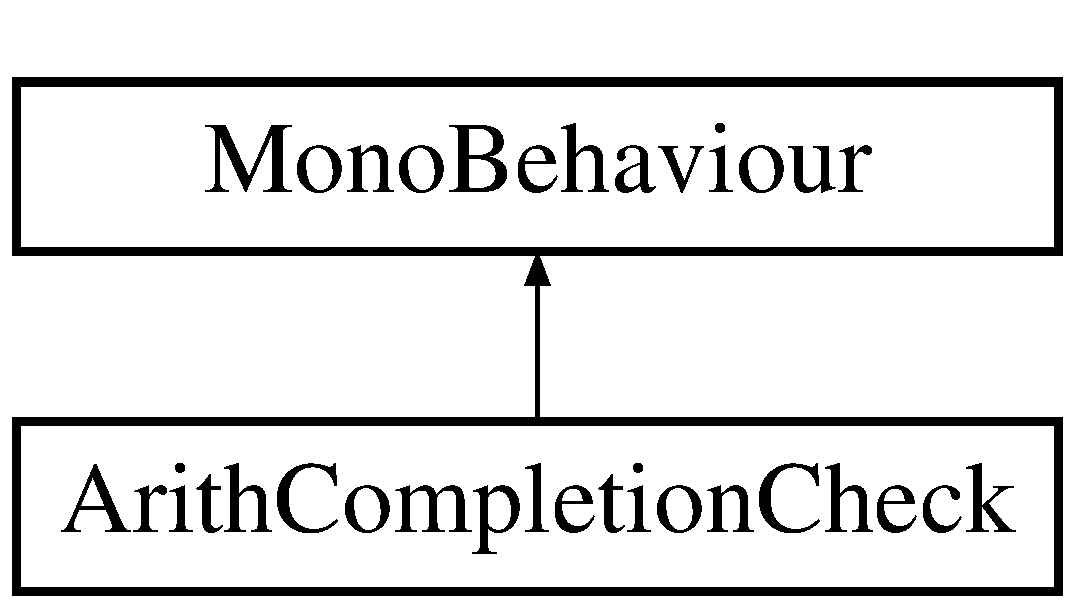
\includegraphics[height=2.000000cm]{class_arith_completion_check}
\end{center}
\end{figure}
\subsection*{Public Member Functions}
\begin{DoxyCompactItemize}
\item 
void \hyperlink{class_arith_completion_check_ab9599e148944886425068a34ae9b236b}{reset\+Puzzle} ()
\item 
void \hyperlink{class_arith_completion_check_a2dd62a0cac8f383172e3a7ef51c3e3a9}{reset\+Check\+Values} ()
\item 
void \hyperlink{class_arith_completion_check_a1499d7cc0dfc5e25ff71ed683a7e1cab}{open\+Door} ()
\item 
void \hyperlink{class_arith_completion_check_a98f38be633381fc1cc645506c854e4c1}{close\+Door} ()
\item 
void \hyperlink{class_arith_completion_check_a43f1f829ee2eb6fd6191c1e76565859b}{reset\+Slots} ()
\begin{DoxyCompactList}\small\item\em reset slots to empty \end{DoxyCompactList}\item 
void \hyperlink{class_arith_completion_check_ab9934c3847957162e5c0bccbe6a47c8c}{reset\+Tiles} ()
\begin{DoxyCompactList}\small\item\em reset tiles to active and in original position \end{DoxyCompactList}\item 
void \hyperlink{class_arith_completion_check_ab96e74dffadaa774579de016d1e4a355}{reset\+Active} ()
\begin{DoxyCompactList}\small\item\em Resets all of the tiles to be active when resetting. \end{DoxyCompactList}\item 
bool \hyperlink{class_arith_completion_check_a29984173a121cf0859ed1a08f4c0e5bd}{check\+Input\+Success} ()
\begin{DoxyCompactList}\small\item\em Checks to be sure that all slots are filled. \end{DoxyCompactList}\item 
bool \hyperlink{class_arith_completion_check_ae813642087af9661c17a03f8545d6f34}{check\+Input\+Name} ()
\begin{DoxyCompactList}\small\item\em Checks to see if the input is correct and in the right order. \end{DoxyCompactList}\end{DoxyCompactItemize}
\subsection*{Public Attributes}
\begin{DoxyCompactItemize}
\item 
Game\+Object \mbox{[}$\,$\mbox{]} \hyperlink{class_arith_completion_check_a29d52d8c29770841ace7a35f5b47f8c7}{check\+Slots}
\begin{DoxyCompactList}\small\item\em manually set in inspector, slots to be filled by tiles \end{DoxyCompactList}\item 
Game\+Object \mbox{[}$\,$\mbox{]} \hyperlink{class_arith_completion_check_a6dd56d93f27bc485fc9354f665a87c2e}{array\+Tiles}
\begin{DoxyCompactList}\small\item\em the tiles that will be dragged \end{DoxyCompactList}\item 
Game\+Object \mbox{[}$\,$\mbox{]} \hyperlink{class_arith_completion_check_a3e4dcde9c1f9660ba26ed864b0a465ac}{replacement\+Tiles}
\begin{DoxyCompactList}\small\item\em The replacement tiles that go into the slots \end{DoxyCompactList}\item 
Game\+Object \hyperlink{class_arith_completion_check_a1ad4ba57922024cef5fc6e788a021f52}{door}
\item 
Audio\+Source \hyperlink{class_arith_completion_check_a3621baade2321e11481457c53e853595}{solved}
\item 
Text \hyperlink{class_arith_completion_check_a715d43af8f5e7b253e9f2da337733d4b}{error\+Message}
\item 
bool \hyperlink{class_arith_completion_check_a11562602e8ce1c9434e869aadf0ac697}{puzzle\+Finished}
\end{DoxyCompactItemize}


\subsection{Member Function Documentation}
\mbox{\Hypertarget{class_arith_completion_check_ae813642087af9661c17a03f8545d6f34}\label{class_arith_completion_check_ae813642087af9661c17a03f8545d6f34}} 
\index{Arith\+Completion\+Check@{Arith\+Completion\+Check}!check\+Input\+Name@{check\+Input\+Name}}
\index{check\+Input\+Name@{check\+Input\+Name}!Arith\+Completion\+Check@{Arith\+Completion\+Check}}
\subsubsection{\texorpdfstring{check\+Input\+Name()}{checkInputName()}}
{\footnotesize\ttfamily bool Arith\+Completion\+Check.\+check\+Input\+Name (\begin{DoxyParamCaption}{ }\end{DoxyParamCaption})}



Checks to see if the input is correct and in the right order. 

\mbox{\Hypertarget{class_arith_completion_check_a29984173a121cf0859ed1a08f4c0e5bd}\label{class_arith_completion_check_a29984173a121cf0859ed1a08f4c0e5bd}} 
\index{Arith\+Completion\+Check@{Arith\+Completion\+Check}!check\+Input\+Success@{check\+Input\+Success}}
\index{check\+Input\+Success@{check\+Input\+Success}!Arith\+Completion\+Check@{Arith\+Completion\+Check}}
\subsubsection{\texorpdfstring{check\+Input\+Success()}{checkInputSuccess()}}
{\footnotesize\ttfamily bool Arith\+Completion\+Check.\+check\+Input\+Success (\begin{DoxyParamCaption}{ }\end{DoxyParamCaption})}



Checks to be sure that all slots are filled. 

\mbox{\Hypertarget{class_arith_completion_check_a98f38be633381fc1cc645506c854e4c1}\label{class_arith_completion_check_a98f38be633381fc1cc645506c854e4c1}} 
\index{Arith\+Completion\+Check@{Arith\+Completion\+Check}!close\+Door@{close\+Door}}
\index{close\+Door@{close\+Door}!Arith\+Completion\+Check@{Arith\+Completion\+Check}}
\subsubsection{\texorpdfstring{close\+Door()}{closeDoor()}}
{\footnotesize\ttfamily void Arith\+Completion\+Check.\+close\+Door (\begin{DoxyParamCaption}{ }\end{DoxyParamCaption})}

\mbox{\Hypertarget{class_arith_completion_check_a1499d7cc0dfc5e25ff71ed683a7e1cab}\label{class_arith_completion_check_a1499d7cc0dfc5e25ff71ed683a7e1cab}} 
\index{Arith\+Completion\+Check@{Arith\+Completion\+Check}!open\+Door@{open\+Door}}
\index{open\+Door@{open\+Door}!Arith\+Completion\+Check@{Arith\+Completion\+Check}}
\subsubsection{\texorpdfstring{open\+Door()}{openDoor()}}
{\footnotesize\ttfamily void Arith\+Completion\+Check.\+open\+Door (\begin{DoxyParamCaption}{ }\end{DoxyParamCaption})}

\mbox{\Hypertarget{class_arith_completion_check_ab96e74dffadaa774579de016d1e4a355}\label{class_arith_completion_check_ab96e74dffadaa774579de016d1e4a355}} 
\index{Arith\+Completion\+Check@{Arith\+Completion\+Check}!reset\+Active@{reset\+Active}}
\index{reset\+Active@{reset\+Active}!Arith\+Completion\+Check@{Arith\+Completion\+Check}}
\subsubsection{\texorpdfstring{reset\+Active()}{resetActive()}}
{\footnotesize\ttfamily void Arith\+Completion\+Check.\+reset\+Active (\begin{DoxyParamCaption}{ }\end{DoxyParamCaption})}



Resets all of the tiles to be active when resetting. 

\mbox{\Hypertarget{class_arith_completion_check_a2dd62a0cac8f383172e3a7ef51c3e3a9}\label{class_arith_completion_check_a2dd62a0cac8f383172e3a7ef51c3e3a9}} 
\index{Arith\+Completion\+Check@{Arith\+Completion\+Check}!reset\+Check\+Values@{reset\+Check\+Values}}
\index{reset\+Check\+Values@{reset\+Check\+Values}!Arith\+Completion\+Check@{Arith\+Completion\+Check}}
\subsubsection{\texorpdfstring{reset\+Check\+Values()}{resetCheckValues()}}
{\footnotesize\ttfamily void Arith\+Completion\+Check.\+reset\+Check\+Values (\begin{DoxyParamCaption}{ }\end{DoxyParamCaption})}

\mbox{\Hypertarget{class_arith_completion_check_ab9599e148944886425068a34ae9b236b}\label{class_arith_completion_check_ab9599e148944886425068a34ae9b236b}} 
\index{Arith\+Completion\+Check@{Arith\+Completion\+Check}!reset\+Puzzle@{reset\+Puzzle}}
\index{reset\+Puzzle@{reset\+Puzzle}!Arith\+Completion\+Check@{Arith\+Completion\+Check}}
\subsubsection{\texorpdfstring{reset\+Puzzle()}{resetPuzzle()}}
{\footnotesize\ttfamily void Arith\+Completion\+Check.\+reset\+Puzzle (\begin{DoxyParamCaption}{ }\end{DoxyParamCaption})}

Resets the puzzle Resets the Tiles, slots, check values, camera flag and error message \mbox{\Hypertarget{class_arith_completion_check_a43f1f829ee2eb6fd6191c1e76565859b}\label{class_arith_completion_check_a43f1f829ee2eb6fd6191c1e76565859b}} 
\index{Arith\+Completion\+Check@{Arith\+Completion\+Check}!reset\+Slots@{reset\+Slots}}
\index{reset\+Slots@{reset\+Slots}!Arith\+Completion\+Check@{Arith\+Completion\+Check}}
\subsubsection{\texorpdfstring{reset\+Slots()}{resetSlots()}}
{\footnotesize\ttfamily void Arith\+Completion\+Check.\+reset\+Slots (\begin{DoxyParamCaption}{ }\end{DoxyParamCaption})}



reset slots to empty 

\mbox{\Hypertarget{class_arith_completion_check_ab9934c3847957162e5c0bccbe6a47c8c}\label{class_arith_completion_check_ab9934c3847957162e5c0bccbe6a47c8c}} 
\index{Arith\+Completion\+Check@{Arith\+Completion\+Check}!reset\+Tiles@{reset\+Tiles}}
\index{reset\+Tiles@{reset\+Tiles}!Arith\+Completion\+Check@{Arith\+Completion\+Check}}
\subsubsection{\texorpdfstring{reset\+Tiles()}{resetTiles()}}
{\footnotesize\ttfamily void Arith\+Completion\+Check.\+reset\+Tiles (\begin{DoxyParamCaption}{ }\end{DoxyParamCaption})}



reset tiles to active and in original position 



\subsection{Member Data Documentation}
\mbox{\Hypertarget{class_arith_completion_check_a6dd56d93f27bc485fc9354f665a87c2e}\label{class_arith_completion_check_a6dd56d93f27bc485fc9354f665a87c2e}} 
\index{Arith\+Completion\+Check@{Arith\+Completion\+Check}!array\+Tiles@{array\+Tiles}}
\index{array\+Tiles@{array\+Tiles}!Arith\+Completion\+Check@{Arith\+Completion\+Check}}
\subsubsection{\texorpdfstring{array\+Tiles}{arrayTiles}}
{\footnotesize\ttfamily Game\+Object \mbox{[}$\,$\mbox{]} Arith\+Completion\+Check.\+array\+Tiles}



the tiles that will be dragged 

\mbox{\Hypertarget{class_arith_completion_check_a29d52d8c29770841ace7a35f5b47f8c7}\label{class_arith_completion_check_a29d52d8c29770841ace7a35f5b47f8c7}} 
\index{Arith\+Completion\+Check@{Arith\+Completion\+Check}!check\+Slots@{check\+Slots}}
\index{check\+Slots@{check\+Slots}!Arith\+Completion\+Check@{Arith\+Completion\+Check}}
\subsubsection{\texorpdfstring{check\+Slots}{checkSlots}}
{\footnotesize\ttfamily Game\+Object \mbox{[}$\,$\mbox{]} Arith\+Completion\+Check.\+check\+Slots}



manually set in inspector, slots to be filled by tiles 

\mbox{\Hypertarget{class_arith_completion_check_a1ad4ba57922024cef5fc6e788a021f52}\label{class_arith_completion_check_a1ad4ba57922024cef5fc6e788a021f52}} 
\index{Arith\+Completion\+Check@{Arith\+Completion\+Check}!door@{door}}
\index{door@{door}!Arith\+Completion\+Check@{Arith\+Completion\+Check}}
\subsubsection{\texorpdfstring{door}{door}}
{\footnotesize\ttfamily Game\+Object Arith\+Completion\+Check.\+door}

\mbox{\Hypertarget{class_arith_completion_check_a715d43af8f5e7b253e9f2da337733d4b}\label{class_arith_completion_check_a715d43af8f5e7b253e9f2da337733d4b}} 
\index{Arith\+Completion\+Check@{Arith\+Completion\+Check}!error\+Message@{error\+Message}}
\index{error\+Message@{error\+Message}!Arith\+Completion\+Check@{Arith\+Completion\+Check}}
\subsubsection{\texorpdfstring{error\+Message}{errorMessage}}
{\footnotesize\ttfamily Text Arith\+Completion\+Check.\+error\+Message}

\mbox{\Hypertarget{class_arith_completion_check_a11562602e8ce1c9434e869aadf0ac697}\label{class_arith_completion_check_a11562602e8ce1c9434e869aadf0ac697}} 
\index{Arith\+Completion\+Check@{Arith\+Completion\+Check}!puzzle\+Finished@{puzzle\+Finished}}
\index{puzzle\+Finished@{puzzle\+Finished}!Arith\+Completion\+Check@{Arith\+Completion\+Check}}
\subsubsection{\texorpdfstring{puzzle\+Finished}{puzzleFinished}}
{\footnotesize\ttfamily bool Arith\+Completion\+Check.\+puzzle\+Finished}

\mbox{\Hypertarget{class_arith_completion_check_a3e4dcde9c1f9660ba26ed864b0a465ac}\label{class_arith_completion_check_a3e4dcde9c1f9660ba26ed864b0a465ac}} 
\index{Arith\+Completion\+Check@{Arith\+Completion\+Check}!replacement\+Tiles@{replacement\+Tiles}}
\index{replacement\+Tiles@{replacement\+Tiles}!Arith\+Completion\+Check@{Arith\+Completion\+Check}}
\subsubsection{\texorpdfstring{replacement\+Tiles}{replacementTiles}}
{\footnotesize\ttfamily Game\+Object \mbox{[}$\,$\mbox{]} Arith\+Completion\+Check.\+replacement\+Tiles}



The replacement tiles that go into the slots 

\mbox{\Hypertarget{class_arith_completion_check_a3621baade2321e11481457c53e853595}\label{class_arith_completion_check_a3621baade2321e11481457c53e853595}} 
\index{Arith\+Completion\+Check@{Arith\+Completion\+Check}!solved@{solved}}
\index{solved@{solved}!Arith\+Completion\+Check@{Arith\+Completion\+Check}}
\subsubsection{\texorpdfstring{solved}{solved}}
{\footnotesize\ttfamily Audio\+Source Arith\+Completion\+Check.\+solved}



The documentation for this class was generated from the following file\+:\begin{DoxyCompactItemize}
\item 
/\+Users/kwanholloway/git/5001\+Project/\+Game\+Project/\+Assets/\+Scripts/\+Puzzle\+Logic/\+Arithmetic\+Puzzle/\hyperlink{_arith_completion_check_8cs}{Arith\+Completion\+Check.\+cs}\end{DoxyCompactItemize}

\hypertarget{classarithmetic_teleporter}{}\section{arithmetic\+Teleporter Class Reference}
\label{classarithmetic_teleporter}\index{arithmetic\+Teleporter@{arithmetic\+Teleporter}}
Inheritance diagram for arithmetic\+Teleporter\+:\begin{figure}[H]
\begin{center}
\leavevmode
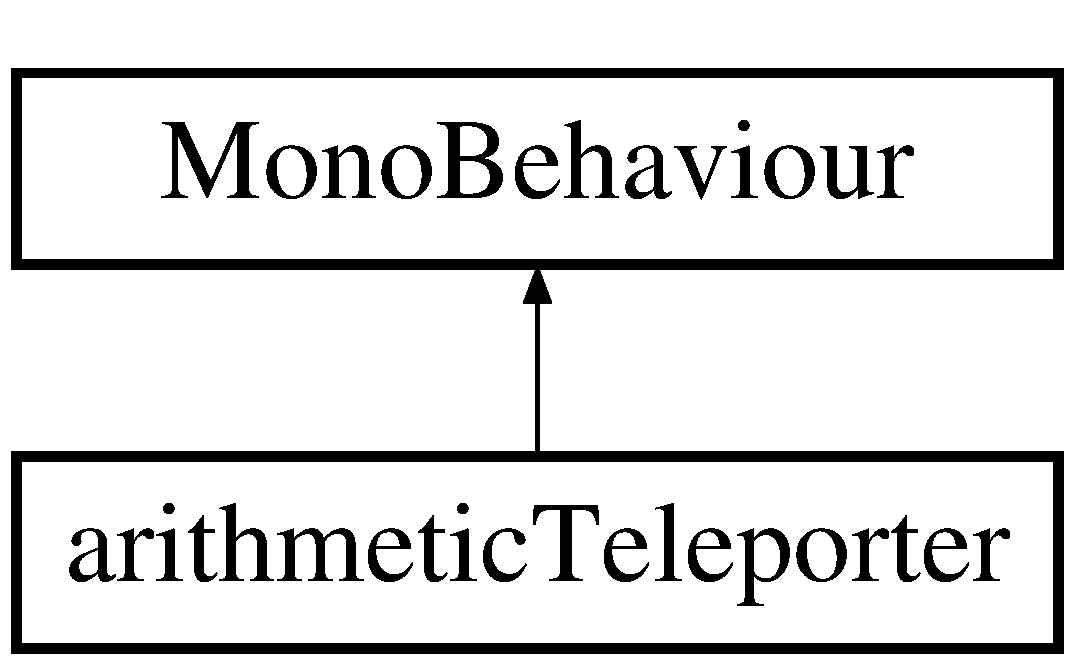
\includegraphics[height=2.000000cm]{classarithmetic_teleporter}
\end{center}
\end{figure}


The documentation for this class was generated from the following file\+:\begin{DoxyCompactItemize}
\item 
/\+Users/kwanholloway/git/5001\+Project/\+Game\+Project/\+Assets/\+Scripts/\+Game\+Logic/\hyperlink{arithmetic_teleporter_8cs}{arithmetic\+Teleporter.\+cs}\end{DoxyCompactItemize}

\hypertarget{class_array_access_completion}{}\section{Array\+Access\+Completion Class Reference}
\label{class_array_access_completion}\index{Array\+Access\+Completion@{Array\+Access\+Completion}}
Inheritance diagram for Array\+Access\+Completion\+:\begin{figure}[H]
\begin{center}
\leavevmode
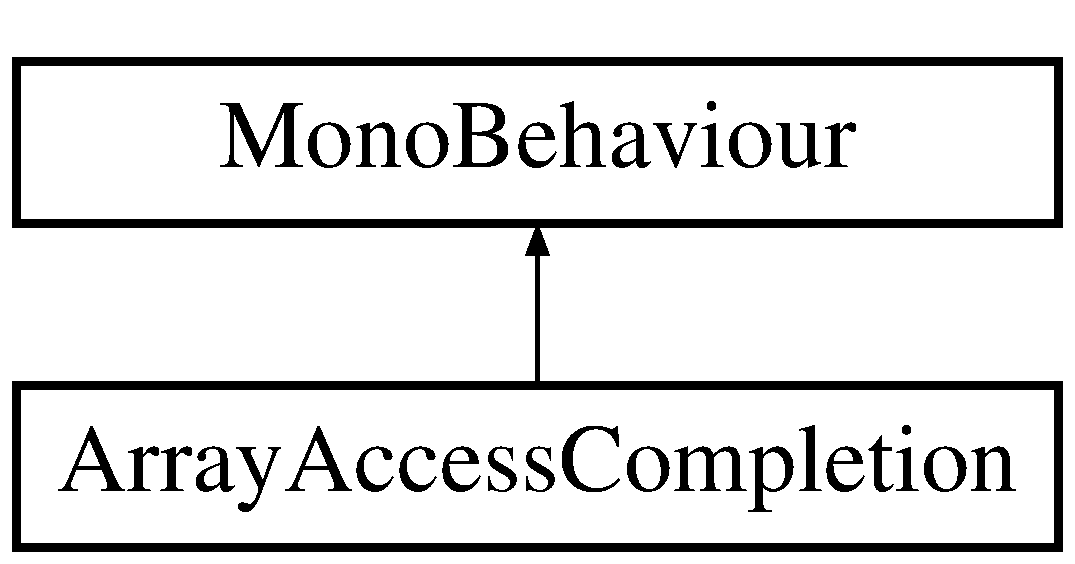
\includegraphics[height=2.000000cm]{class_array_access_completion}
\end{center}
\end{figure}
\subsection*{Public Member Functions}
\begin{DoxyCompactItemize}
\item 
void \hyperlink{class_array_access_completion_a317a8a4cc02701f79003290ba3b00f02}{reset\+Puzzle} ()
\item 
void \hyperlink{class_array_access_completion_a46a4adc2ab93ea43fb9acb31a3770624}{switch\+To\+Error\+Screen} ()
\item 
bool \hyperlink{class_array_access_completion_a16f52bce4f85c9dc5e6f751531988bb0}{error\+Value\+Used} ()
\item 
void \hyperlink{class_array_access_completion_ac2350f79701c5e7a953e44e788347c6c}{reset\+Check\+Values} ()
\item 
void \hyperlink{class_array_access_completion_ac3834cd64df95140d0becf11f7eb15de}{make\+Platforms\+Visible} ()
\item 
void \hyperlink{class_array_access_completion_a7d73c45ea206180019c5cc0e7a73eb92}{reset\+Slots} ()
\item 
void \hyperlink{class_array_access_completion_a0975baec709eab99fa831cefd45a2069}{reset\+Tiles} ()
\item 
void \hyperlink{class_array_access_completion_ac8b88581ac5e6fe71128b6a4c5c64c12}{reset\+Active} ()
\item 
void \hyperlink{class_array_access_completion_af92ecc71a759308e06bf8b4d96ca3c78}{reset\+Platforms} ()
\end{DoxyCompactItemize}
\subsection*{Public Attributes}
\begin{DoxyCompactItemize}
\item 
\hyperlink{class_array_reaction}{Array\+Reaction} \hyperlink{class_array_access_completion_a5b7d8357b6c82703f06eaabee00d0f2f}{check\+One}
\item 
Game\+Object \mbox{[}$\,$\mbox{]} \hyperlink{class_array_access_completion_ae8c88b6f2dd0fe851c866097911df8e4}{array\+Tiles}
\item 
Game\+Object \mbox{[}$\,$\mbox{]} \hyperlink{class_array_access_completion_a97c6ec1f65786273d1186f23ce5b0f6c}{replacement\+Tiles}
\item 
Camera \hyperlink{class_array_access_completion_a0e0e013df2a9203aa27344b6090a56aa}{error\+Cam}
\item 
Text \hyperlink{class_array_access_completion_a03988dc3e4e687e24f0c2c57d75a03b0}{error\+Message}
\item 
bool \hyperlink{class_array_access_completion_a1cddf9521f110a2868afa36514c9dcb4}{puzzle\+Finished}
\end{DoxyCompactItemize}


\subsection{Member Function Documentation}
\mbox{\Hypertarget{class_array_access_completion_a16f52bce4f85c9dc5e6f751531988bb0}\label{class_array_access_completion_a16f52bce4f85c9dc5e6f751531988bb0}} 
\index{Array\+Access\+Completion@{Array\+Access\+Completion}!error\+Value\+Used@{error\+Value\+Used}}
\index{error\+Value\+Used@{error\+Value\+Used}!Array\+Access\+Completion@{Array\+Access\+Completion}}
\subsubsection{\texorpdfstring{error\+Value\+Used()}{errorValueUsed()}}
{\footnotesize\ttfamily bool Array\+Access\+Completion.\+error\+Value\+Used (\begin{DoxyParamCaption}{ }\end{DoxyParamCaption})}

\mbox{\Hypertarget{class_array_access_completion_ac3834cd64df95140d0becf11f7eb15de}\label{class_array_access_completion_ac3834cd64df95140d0becf11f7eb15de}} 
\index{Array\+Access\+Completion@{Array\+Access\+Completion}!make\+Platforms\+Visible@{make\+Platforms\+Visible}}
\index{make\+Platforms\+Visible@{make\+Platforms\+Visible}!Array\+Access\+Completion@{Array\+Access\+Completion}}
\subsubsection{\texorpdfstring{make\+Platforms\+Visible()}{makePlatformsVisible()}}
{\footnotesize\ttfamily void Array\+Access\+Completion.\+make\+Platforms\+Visible (\begin{DoxyParamCaption}{ }\end{DoxyParamCaption})}

\mbox{\Hypertarget{class_array_access_completion_ac8b88581ac5e6fe71128b6a4c5c64c12}\label{class_array_access_completion_ac8b88581ac5e6fe71128b6a4c5c64c12}} 
\index{Array\+Access\+Completion@{Array\+Access\+Completion}!reset\+Active@{reset\+Active}}
\index{reset\+Active@{reset\+Active}!Array\+Access\+Completion@{Array\+Access\+Completion}}
\subsubsection{\texorpdfstring{reset\+Active()}{resetActive()}}
{\footnotesize\ttfamily void Array\+Access\+Completion.\+reset\+Active (\begin{DoxyParamCaption}{ }\end{DoxyParamCaption})}

\mbox{\Hypertarget{class_array_access_completion_ac2350f79701c5e7a953e44e788347c6c}\label{class_array_access_completion_ac2350f79701c5e7a953e44e788347c6c}} 
\index{Array\+Access\+Completion@{Array\+Access\+Completion}!reset\+Check\+Values@{reset\+Check\+Values}}
\index{reset\+Check\+Values@{reset\+Check\+Values}!Array\+Access\+Completion@{Array\+Access\+Completion}}
\subsubsection{\texorpdfstring{reset\+Check\+Values()}{resetCheckValues()}}
{\footnotesize\ttfamily void Array\+Access\+Completion.\+reset\+Check\+Values (\begin{DoxyParamCaption}{ }\end{DoxyParamCaption})}

\mbox{\Hypertarget{class_array_access_completion_af92ecc71a759308e06bf8b4d96ca3c78}\label{class_array_access_completion_af92ecc71a759308e06bf8b4d96ca3c78}} 
\index{Array\+Access\+Completion@{Array\+Access\+Completion}!reset\+Platforms@{reset\+Platforms}}
\index{reset\+Platforms@{reset\+Platforms}!Array\+Access\+Completion@{Array\+Access\+Completion}}
\subsubsection{\texorpdfstring{reset\+Platforms()}{resetPlatforms()}}
{\footnotesize\ttfamily void Array\+Access\+Completion.\+reset\+Platforms (\begin{DoxyParamCaption}{ }\end{DoxyParamCaption})}

\mbox{\Hypertarget{class_array_access_completion_a317a8a4cc02701f79003290ba3b00f02}\label{class_array_access_completion_a317a8a4cc02701f79003290ba3b00f02}} 
\index{Array\+Access\+Completion@{Array\+Access\+Completion}!reset\+Puzzle@{reset\+Puzzle}}
\index{reset\+Puzzle@{reset\+Puzzle}!Array\+Access\+Completion@{Array\+Access\+Completion}}
\subsubsection{\texorpdfstring{reset\+Puzzle()}{resetPuzzle()}}
{\footnotesize\ttfamily void Array\+Access\+Completion.\+reset\+Puzzle (\begin{DoxyParamCaption}{ }\end{DoxyParamCaption})}

Resets the puzzle Resets the Tiles, slots, check values, camera flag and error message \mbox{\Hypertarget{class_array_access_completion_a7d73c45ea206180019c5cc0e7a73eb92}\label{class_array_access_completion_a7d73c45ea206180019c5cc0e7a73eb92}} 
\index{Array\+Access\+Completion@{Array\+Access\+Completion}!reset\+Slots@{reset\+Slots}}
\index{reset\+Slots@{reset\+Slots}!Array\+Access\+Completion@{Array\+Access\+Completion}}
\subsubsection{\texorpdfstring{reset\+Slots()}{resetSlots()}}
{\footnotesize\ttfamily void Array\+Access\+Completion.\+reset\+Slots (\begin{DoxyParamCaption}{ }\end{DoxyParamCaption})}

\mbox{\Hypertarget{class_array_access_completion_a0975baec709eab99fa831cefd45a2069}\label{class_array_access_completion_a0975baec709eab99fa831cefd45a2069}} 
\index{Array\+Access\+Completion@{Array\+Access\+Completion}!reset\+Tiles@{reset\+Tiles}}
\index{reset\+Tiles@{reset\+Tiles}!Array\+Access\+Completion@{Array\+Access\+Completion}}
\subsubsection{\texorpdfstring{reset\+Tiles()}{resetTiles()}}
{\footnotesize\ttfamily void Array\+Access\+Completion.\+reset\+Tiles (\begin{DoxyParamCaption}{ }\end{DoxyParamCaption})}

\mbox{\Hypertarget{class_array_access_completion_a46a4adc2ab93ea43fb9acb31a3770624}\label{class_array_access_completion_a46a4adc2ab93ea43fb9acb31a3770624}} 
\index{Array\+Access\+Completion@{Array\+Access\+Completion}!switch\+To\+Error\+Screen@{switch\+To\+Error\+Screen}}
\index{switch\+To\+Error\+Screen@{switch\+To\+Error\+Screen}!Array\+Access\+Completion@{Array\+Access\+Completion}}
\subsubsection{\texorpdfstring{switch\+To\+Error\+Screen()}{switchToErrorScreen()}}
{\footnotesize\ttfamily void Array\+Access\+Completion.\+switch\+To\+Error\+Screen (\begin{DoxyParamCaption}{ }\end{DoxyParamCaption})}



\subsection{Member Data Documentation}
\mbox{\Hypertarget{class_array_access_completion_ae8c88b6f2dd0fe851c866097911df8e4}\label{class_array_access_completion_ae8c88b6f2dd0fe851c866097911df8e4}} 
\index{Array\+Access\+Completion@{Array\+Access\+Completion}!array\+Tiles@{array\+Tiles}}
\index{array\+Tiles@{array\+Tiles}!Array\+Access\+Completion@{Array\+Access\+Completion}}
\subsubsection{\texorpdfstring{array\+Tiles}{arrayTiles}}
{\footnotesize\ttfamily Game\+Object \mbox{[}$\,$\mbox{]} Array\+Access\+Completion.\+array\+Tiles}

\mbox{\Hypertarget{class_array_access_completion_a5b7d8357b6c82703f06eaabee00d0f2f}\label{class_array_access_completion_a5b7d8357b6c82703f06eaabee00d0f2f}} 
\index{Array\+Access\+Completion@{Array\+Access\+Completion}!check\+One@{check\+One}}
\index{check\+One@{check\+One}!Array\+Access\+Completion@{Array\+Access\+Completion}}
\subsubsection{\texorpdfstring{check\+One}{checkOne}}
{\footnotesize\ttfamily \hyperlink{class_array_reaction}{Array\+Reaction} Array\+Access\+Completion.\+check\+One}

\mbox{\Hypertarget{class_array_access_completion_a0e0e013df2a9203aa27344b6090a56aa}\label{class_array_access_completion_a0e0e013df2a9203aa27344b6090a56aa}} 
\index{Array\+Access\+Completion@{Array\+Access\+Completion}!error\+Cam@{error\+Cam}}
\index{error\+Cam@{error\+Cam}!Array\+Access\+Completion@{Array\+Access\+Completion}}
\subsubsection{\texorpdfstring{error\+Cam}{errorCam}}
{\footnotesize\ttfamily Camera Array\+Access\+Completion.\+error\+Cam}

\mbox{\Hypertarget{class_array_access_completion_a03988dc3e4e687e24f0c2c57d75a03b0}\label{class_array_access_completion_a03988dc3e4e687e24f0c2c57d75a03b0}} 
\index{Array\+Access\+Completion@{Array\+Access\+Completion}!error\+Message@{error\+Message}}
\index{error\+Message@{error\+Message}!Array\+Access\+Completion@{Array\+Access\+Completion}}
\subsubsection{\texorpdfstring{error\+Message}{errorMessage}}
{\footnotesize\ttfamily Text Array\+Access\+Completion.\+error\+Message}

\mbox{\Hypertarget{class_array_access_completion_a1cddf9521f110a2868afa36514c9dcb4}\label{class_array_access_completion_a1cddf9521f110a2868afa36514c9dcb4}} 
\index{Array\+Access\+Completion@{Array\+Access\+Completion}!puzzle\+Finished@{puzzle\+Finished}}
\index{puzzle\+Finished@{puzzle\+Finished}!Array\+Access\+Completion@{Array\+Access\+Completion}}
\subsubsection{\texorpdfstring{puzzle\+Finished}{puzzleFinished}}
{\footnotesize\ttfamily bool Array\+Access\+Completion.\+puzzle\+Finished}

\mbox{\Hypertarget{class_array_access_completion_a97c6ec1f65786273d1186f23ce5b0f6c}\label{class_array_access_completion_a97c6ec1f65786273d1186f23ce5b0f6c}} 
\index{Array\+Access\+Completion@{Array\+Access\+Completion}!replacement\+Tiles@{replacement\+Tiles}}
\index{replacement\+Tiles@{replacement\+Tiles}!Array\+Access\+Completion@{Array\+Access\+Completion}}
\subsubsection{\texorpdfstring{replacement\+Tiles}{replacementTiles}}
{\footnotesize\ttfamily Game\+Object \mbox{[}$\,$\mbox{]} Array\+Access\+Completion.\+replacement\+Tiles}



The documentation for this class was generated from the following file\+:\begin{DoxyCompactItemize}
\item 
/\+Users/kwanholloway/git/5001\+Project/\+Game\+Project/\+Assets/\+Scripts/\+Puzzle\+Logic/\+Array\+Access\+Puzzle/\hyperlink{_array_access_completion_8cs}{Array\+Access\+Completion.\+cs}\end{DoxyCompactItemize}

\hypertarget{class_array_box_controller}{}\section{Array\+Box\+Controller Class Reference}
\label{class_array_box_controller}\index{Array\+Box\+Controller@{Array\+Box\+Controller}}
Inheritance diagram for Array\+Box\+Controller\+:\begin{figure}[H]
\begin{center}
\leavevmode
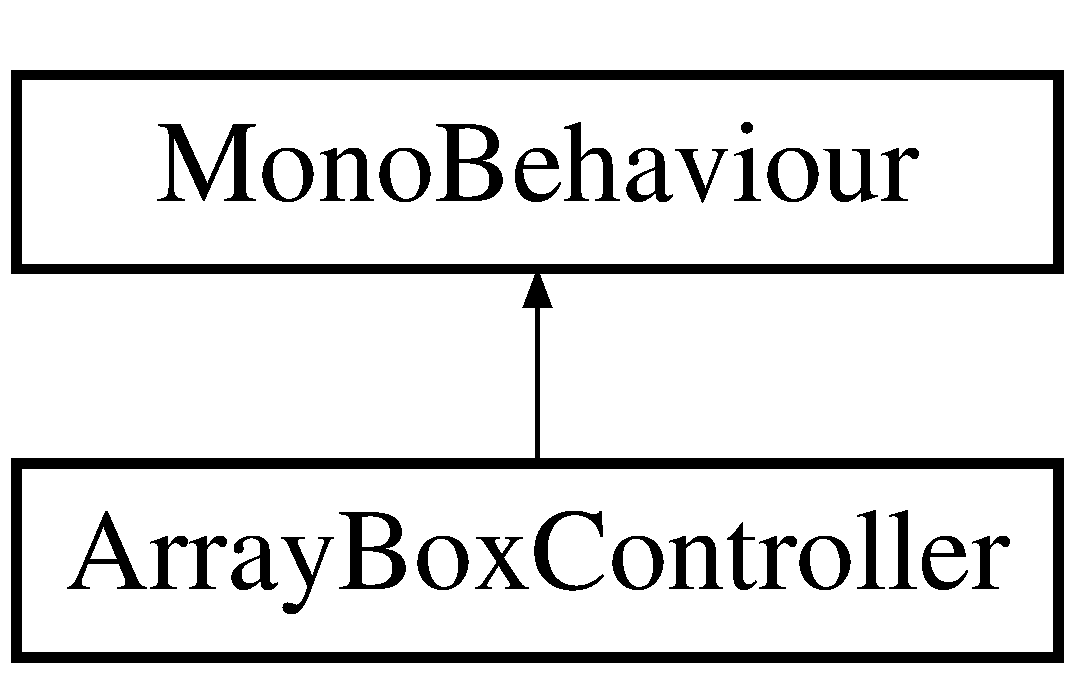
\includegraphics[height=2.000000cm]{class_array_box_controller}
\end{center}
\end{figure}
\subsection*{Public Member Functions}
\begin{DoxyCompactItemize}
\item 
int \hyperlink{class_array_box_controller_aca5b840fdc879a3268c9a57a439d6172}{get\+Weight} ()
\item 
void \hyperlink{class_array_box_controller_a926861290e0d8414a771456f9d573659}{drop\+Platform} ()
\item 
void \hyperlink{class_array_box_controller_aaee7f59464d3cddf435e9669faacd8aa}{create\+Platform} ()
\item 
void \hyperlink{class_array_box_controller_a457e96d6ccf856144d580f392dcc17e8}{reset\+Box} ()
\end{DoxyCompactItemize}
\subsection*{Public Attributes}
\begin{DoxyCompactItemize}
\item 
int \hyperlink{class_array_box_controller_a0703f2b4690bc71070aa58210187a4f5}{weight}
\item 
Game\+Object \hyperlink{class_array_box_controller_a7d14b3ed04e57ed25f856c76bc91bba3}{under\+Platform}
\item 
bool \hyperlink{class_array_box_controller_af7f266ad7922670c221e4a2247308f03}{remove\+Platform}
\item 
bool \hyperlink{class_array_box_controller_a788b69c1dd5fd14ada59788891a50ec2}{slot\+One\+Success}
\end{DoxyCompactItemize}


\subsection{Member Function Documentation}
\mbox{\Hypertarget{class_array_box_controller_aaee7f59464d3cddf435e9669faacd8aa}\label{class_array_box_controller_aaee7f59464d3cddf435e9669faacd8aa}} 
\index{Array\+Box\+Controller@{Array\+Box\+Controller}!create\+Platform@{create\+Platform}}
\index{create\+Platform@{create\+Platform}!Array\+Box\+Controller@{Array\+Box\+Controller}}
\subsubsection{\texorpdfstring{create\+Platform()}{createPlatform()}}
{\footnotesize\ttfamily void Array\+Box\+Controller.\+create\+Platform (\begin{DoxyParamCaption}{ }\end{DoxyParamCaption})}

\mbox{\Hypertarget{class_array_box_controller_a926861290e0d8414a771456f9d573659}\label{class_array_box_controller_a926861290e0d8414a771456f9d573659}} 
\index{Array\+Box\+Controller@{Array\+Box\+Controller}!drop\+Platform@{drop\+Platform}}
\index{drop\+Platform@{drop\+Platform}!Array\+Box\+Controller@{Array\+Box\+Controller}}
\subsubsection{\texorpdfstring{drop\+Platform()}{dropPlatform()}}
{\footnotesize\ttfamily void Array\+Box\+Controller.\+drop\+Platform (\begin{DoxyParamCaption}{ }\end{DoxyParamCaption})}

\mbox{\Hypertarget{class_array_box_controller_aca5b840fdc879a3268c9a57a439d6172}\label{class_array_box_controller_aca5b840fdc879a3268c9a57a439d6172}} 
\index{Array\+Box\+Controller@{Array\+Box\+Controller}!get\+Weight@{get\+Weight}}
\index{get\+Weight@{get\+Weight}!Array\+Box\+Controller@{Array\+Box\+Controller}}
\subsubsection{\texorpdfstring{get\+Weight()}{getWeight()}}
{\footnotesize\ttfamily int Array\+Box\+Controller.\+get\+Weight (\begin{DoxyParamCaption}{ }\end{DoxyParamCaption})}

\mbox{\Hypertarget{class_array_box_controller_a457e96d6ccf856144d580f392dcc17e8}\label{class_array_box_controller_a457e96d6ccf856144d580f392dcc17e8}} 
\index{Array\+Box\+Controller@{Array\+Box\+Controller}!reset\+Box@{reset\+Box}}
\index{reset\+Box@{reset\+Box}!Array\+Box\+Controller@{Array\+Box\+Controller}}
\subsubsection{\texorpdfstring{reset\+Box()}{resetBox()}}
{\footnotesize\ttfamily void Array\+Box\+Controller.\+reset\+Box (\begin{DoxyParamCaption}{ }\end{DoxyParamCaption})}



\subsection{Member Data Documentation}
\mbox{\Hypertarget{class_array_box_controller_af7f266ad7922670c221e4a2247308f03}\label{class_array_box_controller_af7f266ad7922670c221e4a2247308f03}} 
\index{Array\+Box\+Controller@{Array\+Box\+Controller}!remove\+Platform@{remove\+Platform}}
\index{remove\+Platform@{remove\+Platform}!Array\+Box\+Controller@{Array\+Box\+Controller}}
\subsubsection{\texorpdfstring{remove\+Platform}{removePlatform}}
{\footnotesize\ttfamily bool Array\+Box\+Controller.\+remove\+Platform}

\mbox{\Hypertarget{class_array_box_controller_a788b69c1dd5fd14ada59788891a50ec2}\label{class_array_box_controller_a788b69c1dd5fd14ada59788891a50ec2}} 
\index{Array\+Box\+Controller@{Array\+Box\+Controller}!slot\+One\+Success@{slot\+One\+Success}}
\index{slot\+One\+Success@{slot\+One\+Success}!Array\+Box\+Controller@{Array\+Box\+Controller}}
\subsubsection{\texorpdfstring{slot\+One\+Success}{slotOneSuccess}}
{\footnotesize\ttfamily bool Array\+Box\+Controller.\+slot\+One\+Success}

\mbox{\Hypertarget{class_array_box_controller_a7d14b3ed04e57ed25f856c76bc91bba3}\label{class_array_box_controller_a7d14b3ed04e57ed25f856c76bc91bba3}} 
\index{Array\+Box\+Controller@{Array\+Box\+Controller}!under\+Platform@{under\+Platform}}
\index{under\+Platform@{under\+Platform}!Array\+Box\+Controller@{Array\+Box\+Controller}}
\subsubsection{\texorpdfstring{under\+Platform}{underPlatform}}
{\footnotesize\ttfamily Game\+Object Array\+Box\+Controller.\+under\+Platform}

\mbox{\Hypertarget{class_array_box_controller_a0703f2b4690bc71070aa58210187a4f5}\label{class_array_box_controller_a0703f2b4690bc71070aa58210187a4f5}} 
\index{Array\+Box\+Controller@{Array\+Box\+Controller}!weight@{weight}}
\index{weight@{weight}!Array\+Box\+Controller@{Array\+Box\+Controller}}
\subsubsection{\texorpdfstring{weight}{weight}}
{\footnotesize\ttfamily int Array\+Box\+Controller.\+weight}



The documentation for this class was generated from the following file\+:\begin{DoxyCompactItemize}
\item 
/\+Users/kwanholloway/git/5001\+Project/\+Game\+Project/\+Assets/\+Scripts/\+Array\+Puzzle\+One/\hyperlink{_array_box_controller_8cs}{Array\+Box\+Controller.\+cs}\end{DoxyCompactItemize}

\hypertarget{class_array_reaction}{}\section{Array\+Reaction Class Reference}
\label{class_array_reaction}\index{Array\+Reaction@{Array\+Reaction}}
Inheritance diagram for Array\+Reaction\+:\begin{figure}[H]
\begin{center}
\leavevmode
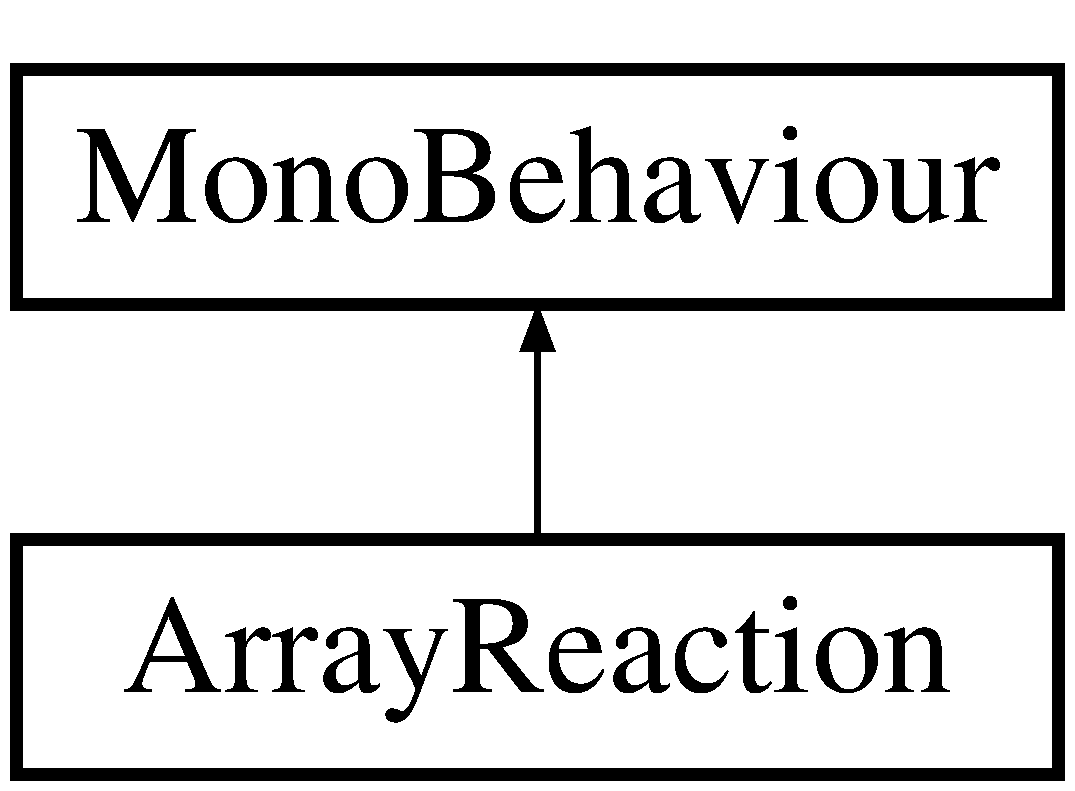
\includegraphics[height=2.000000cm]{class_array_reaction}
\end{center}
\end{figure}
\subsection*{Public Member Functions}
\begin{DoxyCompactItemize}
\item 
void \hyperlink{class_array_reaction_ab805c31627d8e16a92813afad4a6e7bb}{reset\+Success\+Bool} ()
\end{DoxyCompactItemize}
\subsection*{Public Attributes}
\begin{DoxyCompactItemize}
\item 
bool \hyperlink{class_array_reaction_adf5df12cecfb640661571ae871e5be5d}{success}
\item 
string \hyperlink{class_array_reaction_aab057c39f78c1f0f9a2cacf8a7d23f6f}{give\+Name}
\item 
Audio\+Source \hyperlink{class_array_reaction_ad469f4e03562bf0773db8ca308997a10}{correct}
\end{DoxyCompactItemize}


\subsection{Member Function Documentation}
\mbox{\Hypertarget{class_array_reaction_ab805c31627d8e16a92813afad4a6e7bb}\label{class_array_reaction_ab805c31627d8e16a92813afad4a6e7bb}} 
\index{Array\+Reaction@{Array\+Reaction}!reset\+Success\+Bool@{reset\+Success\+Bool}}
\index{reset\+Success\+Bool@{reset\+Success\+Bool}!Array\+Reaction@{Array\+Reaction}}
\subsubsection{\texorpdfstring{reset\+Success\+Bool()}{resetSuccessBool()}}
{\footnotesize\ttfamily void Array\+Reaction.\+reset\+Success\+Bool (\begin{DoxyParamCaption}{ }\end{DoxyParamCaption})}



\subsection{Member Data Documentation}
\mbox{\Hypertarget{class_array_reaction_ad469f4e03562bf0773db8ca308997a10}\label{class_array_reaction_ad469f4e03562bf0773db8ca308997a10}} 
\index{Array\+Reaction@{Array\+Reaction}!correct@{correct}}
\index{correct@{correct}!Array\+Reaction@{Array\+Reaction}}
\subsubsection{\texorpdfstring{correct}{correct}}
{\footnotesize\ttfamily Audio\+Source Array\+Reaction.\+correct}

\mbox{\Hypertarget{class_array_reaction_aab057c39f78c1f0f9a2cacf8a7d23f6f}\label{class_array_reaction_aab057c39f78c1f0f9a2cacf8a7d23f6f}} 
\index{Array\+Reaction@{Array\+Reaction}!give\+Name@{give\+Name}}
\index{give\+Name@{give\+Name}!Array\+Reaction@{Array\+Reaction}}
\subsubsection{\texorpdfstring{give\+Name}{giveName}}
{\footnotesize\ttfamily string Array\+Reaction.\+give\+Name}

\mbox{\Hypertarget{class_array_reaction_adf5df12cecfb640661571ae871e5be5d}\label{class_array_reaction_adf5df12cecfb640661571ae871e5be5d}} 
\index{Array\+Reaction@{Array\+Reaction}!success@{success}}
\index{success@{success}!Array\+Reaction@{Array\+Reaction}}
\subsubsection{\texorpdfstring{success}{success}}
{\footnotesize\ttfamily bool Array\+Reaction.\+success}



The documentation for this class was generated from the following file\+:\begin{DoxyCompactItemize}
\item 
/\+Users/kwanholloway/git/5001\+Project/\+Game\+Project/\+Assets/\+Scripts/\+Puzzle\+Logic/\+Array\+Sumation\+Puzzle/\hyperlink{_array_reaction_8cs}{Array\+Reaction.\+cs}\end{DoxyCompactItemize}

\hypertarget{class_array_sum_completion}{}\section{Array\+Sum\+Completion Class Reference}
\label{class_array_sum_completion}\index{Array\+Sum\+Completion@{Array\+Sum\+Completion}}
Inheritance diagram for Array\+Sum\+Completion\+:\begin{figure}[H]
\begin{center}
\leavevmode
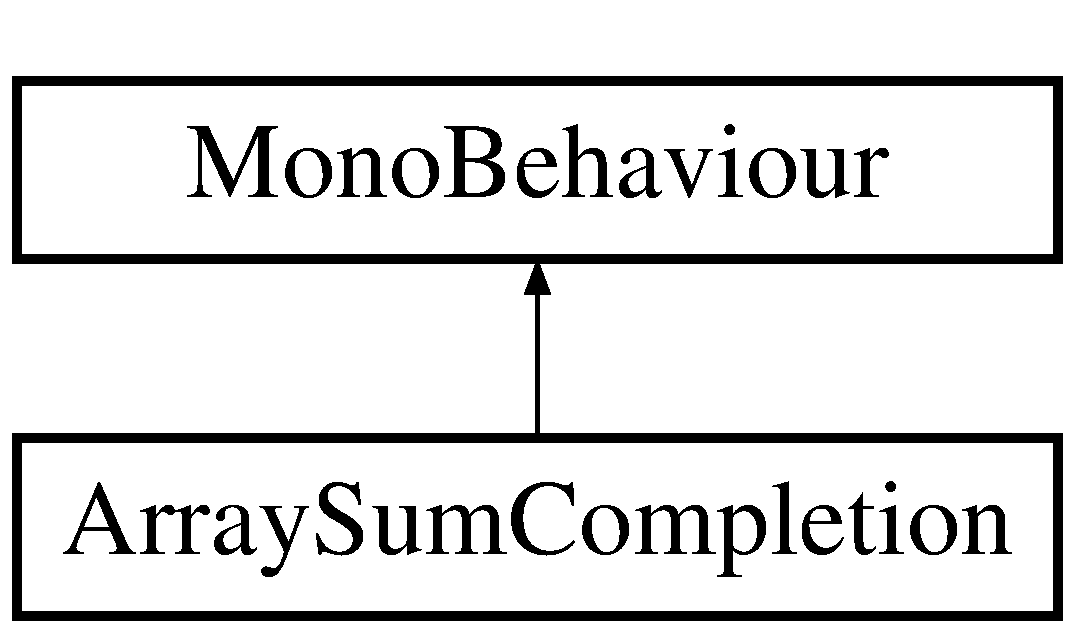
\includegraphics[height=2.000000cm]{class_array_sum_completion}
\end{center}
\end{figure}
\subsection*{Public Member Functions}
\begin{DoxyCompactItemize}
\item 
void \hyperlink{class_array_sum_completion_a7ebbac41382a93bf539032555a3c9bd9}{reset\+Puzzle} ()
\item 
void \hyperlink{class_array_sum_completion_a3ae23072215cde0cdce19c8f8b773b7b}{reset\+Check\+Values} ()
\item 
void \hyperlink{class_array_sum_completion_ac1c819eeab2598e8c2c2e1e78e15a666}{drop\+Tile\+Platforms} ()
\item 
void \hyperlink{class_array_sum_completion_a033797d55e28346be6d4821f3bdc2daa}{reset\+Slots} ()
\begin{DoxyCompactList}\small\item\em reset slots to empty \end{DoxyCompactList}\item 
void \hyperlink{class_array_sum_completion_a9219153273ef00f35c1ccb98cf408af3}{reset\+Tiles} ()
\begin{DoxyCompactList}\small\item\em reset tiles to active and in original position \end{DoxyCompactList}\item 
void \hyperlink{class_array_sum_completion_a9c8cbe4d07015cd0e6c958e39e0e92d2}{reset\+Active} ()
\begin{DoxyCompactList}\small\item\em Resets all of the tiles to be active when resetting. \end{DoxyCompactList}\item 
void \hyperlink{class_array_sum_completion_a1289c469259345582c0227f7a617a19f}{reset\+Boxes\+And\+Platforms} ()
\begin{DoxyCompactList}\small\item\em Places the boxes and their platforms back at the starting postions to be used again. \end{DoxyCompactList}\end{DoxyCompactItemize}
\subsection*{Public Attributes}
\begin{DoxyCompactItemize}
\item 
\hyperlink{class_array_reaction}{Array\+Reaction} \hyperlink{class_array_sum_completion_ac76237e402fcc0e49a59a6e87c5def61}{check\+One}
\begin{DoxyCompactList}\small\item\em The slots that will be checked \end{DoxyCompactList}\item 
Game\+Object \hyperlink{class_array_sum_completion_aede79dd24168cb27103df95c78a78abf}{rising\+Platform}
\begin{DoxyCompactList}\small\item\em rising counter-\/weight platform \end{DoxyCompactList}\item 
Game\+Object \mbox{[}$\,$\mbox{]} \hyperlink{class_array_sum_completion_a18c8b02ee9ab7e991e7e49e97540794b}{array\+Tiles}
\begin{DoxyCompactList}\small\item\em the tiles that will be dragged \end{DoxyCompactList}\item 
Game\+Object \mbox{[}$\,$\mbox{]} \hyperlink{class_array_sum_completion_a51878c1ec6f821a4d7adff431b4143d1}{replacement\+Tiles}
\begin{DoxyCompactList}\small\item\em The replacement tiles that go into the slots \end{DoxyCompactList}\item 
List$<$ Vector3 $>$ \hyperlink{class_array_sum_completion_a48661584c0748edee316371617b45b5d}{array\+Tile\+Positions}
\begin{DoxyCompactList}\small\item\em their positions, used for resetting challenge \end{DoxyCompactList}\item 
bool \hyperlink{class_array_sum_completion_acbefffe0c43bbd4cd21cfcf34e0a9b7c}{puzzle\+Finished}
\begin{DoxyCompactList}\small\item\em Bools to detect if the puzzle is done and the camera was toggled. Used in resetting and toggling of the camera \end{DoxyCompactList}\end{DoxyCompactItemize}


\subsection{Detailed Description}
Checks the respective challenge and makes changes to the game if the user is correct or not Challenge\+: Array challenge 2 

\subsection{Member Function Documentation}
\mbox{\Hypertarget{class_array_sum_completion_ac1c819eeab2598e8c2c2e1e78e15a666}\label{class_array_sum_completion_ac1c819eeab2598e8c2c2e1e78e15a666}} 
\index{Array\+Sum\+Completion@{Array\+Sum\+Completion}!drop\+Tile\+Platforms@{drop\+Tile\+Platforms}}
\index{drop\+Tile\+Platforms@{drop\+Tile\+Platforms}!Array\+Sum\+Completion@{Array\+Sum\+Completion}}
\subsubsection{\texorpdfstring{drop\+Tile\+Platforms()}{dropTilePlatforms()}}
{\footnotesize\ttfamily void Array\+Sum\+Completion.\+drop\+Tile\+Platforms (\begin{DoxyParamCaption}{ }\end{DoxyParamCaption})}

Calls each Box\textquotesingle{}s method to let them fall for the weight challenge \mbox{\Hypertarget{class_array_sum_completion_a9c8cbe4d07015cd0e6c958e39e0e92d2}\label{class_array_sum_completion_a9c8cbe4d07015cd0e6c958e39e0e92d2}} 
\index{Array\+Sum\+Completion@{Array\+Sum\+Completion}!reset\+Active@{reset\+Active}}
\index{reset\+Active@{reset\+Active}!Array\+Sum\+Completion@{Array\+Sum\+Completion}}
\subsubsection{\texorpdfstring{reset\+Active()}{resetActive()}}
{\footnotesize\ttfamily void Array\+Sum\+Completion.\+reset\+Active (\begin{DoxyParamCaption}{ }\end{DoxyParamCaption})}



Resets all of the tiles to be active when resetting. 

\mbox{\Hypertarget{class_array_sum_completion_a1289c469259345582c0227f7a617a19f}\label{class_array_sum_completion_a1289c469259345582c0227f7a617a19f}} 
\index{Array\+Sum\+Completion@{Array\+Sum\+Completion}!reset\+Boxes\+And\+Platforms@{reset\+Boxes\+And\+Platforms}}
\index{reset\+Boxes\+And\+Platforms@{reset\+Boxes\+And\+Platforms}!Array\+Sum\+Completion@{Array\+Sum\+Completion}}
\subsubsection{\texorpdfstring{reset\+Boxes\+And\+Platforms()}{resetBoxesAndPlatforms()}}
{\footnotesize\ttfamily void Array\+Sum\+Completion.\+reset\+Boxes\+And\+Platforms (\begin{DoxyParamCaption}{ }\end{DoxyParamCaption})}



Places the boxes and their platforms back at the starting postions to be used again. 

\mbox{\Hypertarget{class_array_sum_completion_a3ae23072215cde0cdce19c8f8b773b7b}\label{class_array_sum_completion_a3ae23072215cde0cdce19c8f8b773b7b}} 
\index{Array\+Sum\+Completion@{Array\+Sum\+Completion}!reset\+Check\+Values@{reset\+Check\+Values}}
\index{reset\+Check\+Values@{reset\+Check\+Values}!Array\+Sum\+Completion@{Array\+Sum\+Completion}}
\subsubsection{\texorpdfstring{reset\+Check\+Values()}{resetCheckValues()}}
{\footnotesize\ttfamily void Array\+Sum\+Completion.\+reset\+Check\+Values (\begin{DoxyParamCaption}{ }\end{DoxyParamCaption})}

Resets the slot\textquotesingle{}s success bools so they can be used again \mbox{\Hypertarget{class_array_sum_completion_a7ebbac41382a93bf539032555a3c9bd9}\label{class_array_sum_completion_a7ebbac41382a93bf539032555a3c9bd9}} 
\index{Array\+Sum\+Completion@{Array\+Sum\+Completion}!reset\+Puzzle@{reset\+Puzzle}}
\index{reset\+Puzzle@{reset\+Puzzle}!Array\+Sum\+Completion@{Array\+Sum\+Completion}}
\subsubsection{\texorpdfstring{reset\+Puzzle()}{resetPuzzle()}}
{\footnotesize\ttfamily void Array\+Sum\+Completion.\+reset\+Puzzle (\begin{DoxyParamCaption}{ }\end{DoxyParamCaption})}

Resets the puzzle Resets the Tiles, slots, check values, camera flag and error message \mbox{\Hypertarget{class_array_sum_completion_a033797d55e28346be6d4821f3bdc2daa}\label{class_array_sum_completion_a033797d55e28346be6d4821f3bdc2daa}} 
\index{Array\+Sum\+Completion@{Array\+Sum\+Completion}!reset\+Slots@{reset\+Slots}}
\index{reset\+Slots@{reset\+Slots}!Array\+Sum\+Completion@{Array\+Sum\+Completion}}
\subsubsection{\texorpdfstring{reset\+Slots()}{resetSlots()}}
{\footnotesize\ttfamily void Array\+Sum\+Completion.\+reset\+Slots (\begin{DoxyParamCaption}{ }\end{DoxyParamCaption})}



reset slots to empty 

\mbox{\Hypertarget{class_array_sum_completion_a9219153273ef00f35c1ccb98cf408af3}\label{class_array_sum_completion_a9219153273ef00f35c1ccb98cf408af3}} 
\index{Array\+Sum\+Completion@{Array\+Sum\+Completion}!reset\+Tiles@{reset\+Tiles}}
\index{reset\+Tiles@{reset\+Tiles}!Array\+Sum\+Completion@{Array\+Sum\+Completion}}
\subsubsection{\texorpdfstring{reset\+Tiles()}{resetTiles()}}
{\footnotesize\ttfamily void Array\+Sum\+Completion.\+reset\+Tiles (\begin{DoxyParamCaption}{ }\end{DoxyParamCaption})}



reset tiles to active and in original position 



\subsection{Member Data Documentation}
\mbox{\Hypertarget{class_array_sum_completion_a48661584c0748edee316371617b45b5d}\label{class_array_sum_completion_a48661584c0748edee316371617b45b5d}} 
\index{Array\+Sum\+Completion@{Array\+Sum\+Completion}!array\+Tile\+Positions@{array\+Tile\+Positions}}
\index{array\+Tile\+Positions@{array\+Tile\+Positions}!Array\+Sum\+Completion@{Array\+Sum\+Completion}}
\subsubsection{\texorpdfstring{array\+Tile\+Positions}{arrayTilePositions}}
{\footnotesize\ttfamily List$<$Vector3$>$ Array\+Sum\+Completion.\+array\+Tile\+Positions}



their positions, used for resetting challenge 

\mbox{\Hypertarget{class_array_sum_completion_a18c8b02ee9ab7e991e7e49e97540794b}\label{class_array_sum_completion_a18c8b02ee9ab7e991e7e49e97540794b}} 
\index{Array\+Sum\+Completion@{Array\+Sum\+Completion}!array\+Tiles@{array\+Tiles}}
\index{array\+Tiles@{array\+Tiles}!Array\+Sum\+Completion@{Array\+Sum\+Completion}}
\subsubsection{\texorpdfstring{array\+Tiles}{arrayTiles}}
{\footnotesize\ttfamily Game\+Object \mbox{[}$\,$\mbox{]} Array\+Sum\+Completion.\+array\+Tiles}



the tiles that will be dragged 

\mbox{\Hypertarget{class_array_sum_completion_ac76237e402fcc0e49a59a6e87c5def61}\label{class_array_sum_completion_ac76237e402fcc0e49a59a6e87c5def61}} 
\index{Array\+Sum\+Completion@{Array\+Sum\+Completion}!check\+One@{check\+One}}
\index{check\+One@{check\+One}!Array\+Sum\+Completion@{Array\+Sum\+Completion}}
\subsubsection{\texorpdfstring{check\+One}{checkOne}}
{\footnotesize\ttfamily \hyperlink{class_array_reaction}{Array\+Reaction} Array\+Sum\+Completion.\+check\+One}



The slots that will be checked 

\mbox{\Hypertarget{class_array_sum_completion_acbefffe0c43bbd4cd21cfcf34e0a9b7c}\label{class_array_sum_completion_acbefffe0c43bbd4cd21cfcf34e0a9b7c}} 
\index{Array\+Sum\+Completion@{Array\+Sum\+Completion}!puzzle\+Finished@{puzzle\+Finished}}
\index{puzzle\+Finished@{puzzle\+Finished}!Array\+Sum\+Completion@{Array\+Sum\+Completion}}
\subsubsection{\texorpdfstring{puzzle\+Finished}{puzzleFinished}}
{\footnotesize\ttfamily bool Array\+Sum\+Completion.\+puzzle\+Finished}



Bools to detect if the puzzle is done and the camera was toggled. Used in resetting and toggling of the camera 

\mbox{\Hypertarget{class_array_sum_completion_a51878c1ec6f821a4d7adff431b4143d1}\label{class_array_sum_completion_a51878c1ec6f821a4d7adff431b4143d1}} 
\index{Array\+Sum\+Completion@{Array\+Sum\+Completion}!replacement\+Tiles@{replacement\+Tiles}}
\index{replacement\+Tiles@{replacement\+Tiles}!Array\+Sum\+Completion@{Array\+Sum\+Completion}}
\subsubsection{\texorpdfstring{replacement\+Tiles}{replacementTiles}}
{\footnotesize\ttfamily Game\+Object \mbox{[}$\,$\mbox{]} Array\+Sum\+Completion.\+replacement\+Tiles}



The replacement tiles that go into the slots 

\mbox{\Hypertarget{class_array_sum_completion_aede79dd24168cb27103df95c78a78abf}\label{class_array_sum_completion_aede79dd24168cb27103df95c78a78abf}} 
\index{Array\+Sum\+Completion@{Array\+Sum\+Completion}!rising\+Platform@{rising\+Platform}}
\index{rising\+Platform@{rising\+Platform}!Array\+Sum\+Completion@{Array\+Sum\+Completion}}
\subsubsection{\texorpdfstring{rising\+Platform}{risingPlatform}}
{\footnotesize\ttfamily Game\+Object Array\+Sum\+Completion.\+rising\+Platform}



rising counter-\/weight platform 



The documentation for this class was generated from the following file\+:\begin{DoxyCompactItemize}
\item 
/\+Users/kwanholloway/git/5001\+Project/\+Game\+Project/\+Assets/\+Scripts/\+Puzzle\+Logic/\+Array\+Sumation\+Puzzle/\hyperlink{_array_sum_completion_8cs}{Array\+Sum\+Completion.\+cs}\end{DoxyCompactItemize}

\hypertarget{class_array_teleporter}{}\section{Array\+Teleporter Class Reference}
\label{class_array_teleporter}\index{Array\+Teleporter@{Array\+Teleporter}}
Inheritance diagram for Array\+Teleporter\+:\begin{figure}[H]
\begin{center}
\leavevmode
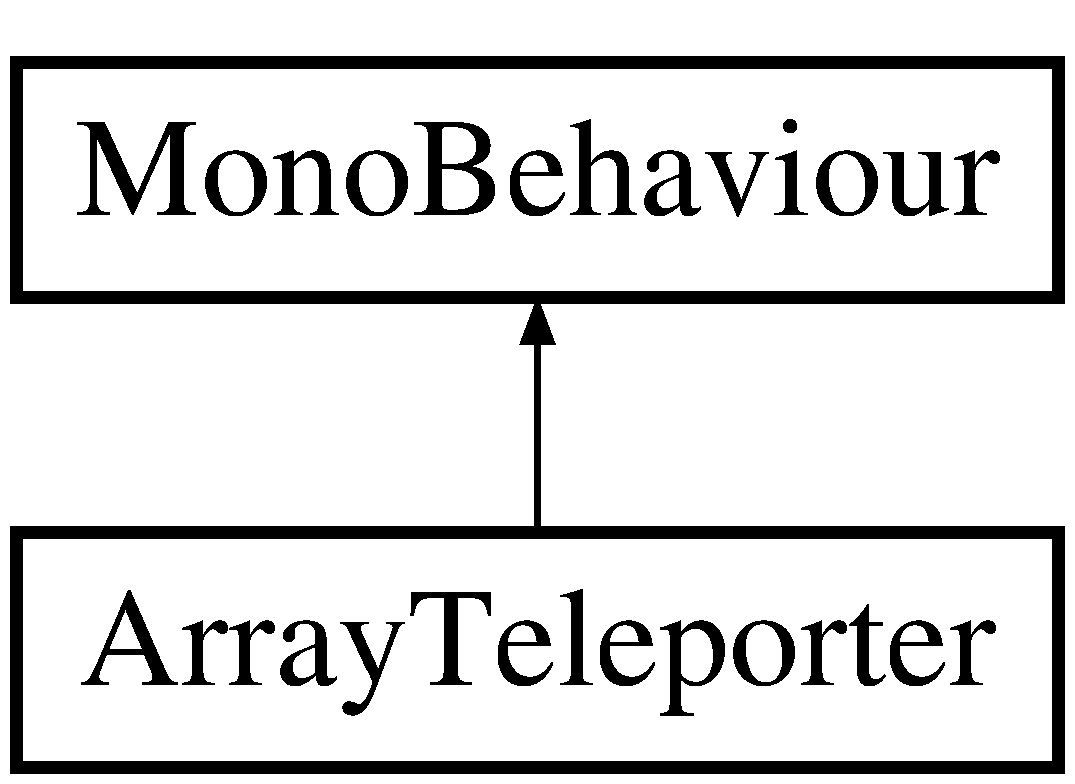
\includegraphics[height=2.000000cm]{class_array_teleporter}
\end{center}
\end{figure}


The documentation for this class was generated from the following file\+:\begin{DoxyCompactItemize}
\item 
/\+Users/kwanholloway/git/5001\+Project/\+Game\+Project/\+Assets/\+Scripts/\+Game\+Logic/\hyperlink{_array_teleporter_8cs}{Array\+Teleporter.\+cs}\end{DoxyCompactItemize}

\hypertarget{class_array_tile_controller}{}\section{Array\+Tile\+Controller Class Reference}
\label{class_array_tile_controller}\index{Array\+Tile\+Controller@{Array\+Tile\+Controller}}
Inheritance diagram for Array\+Tile\+Controller\+:\begin{figure}[H]
\begin{center}
\leavevmode
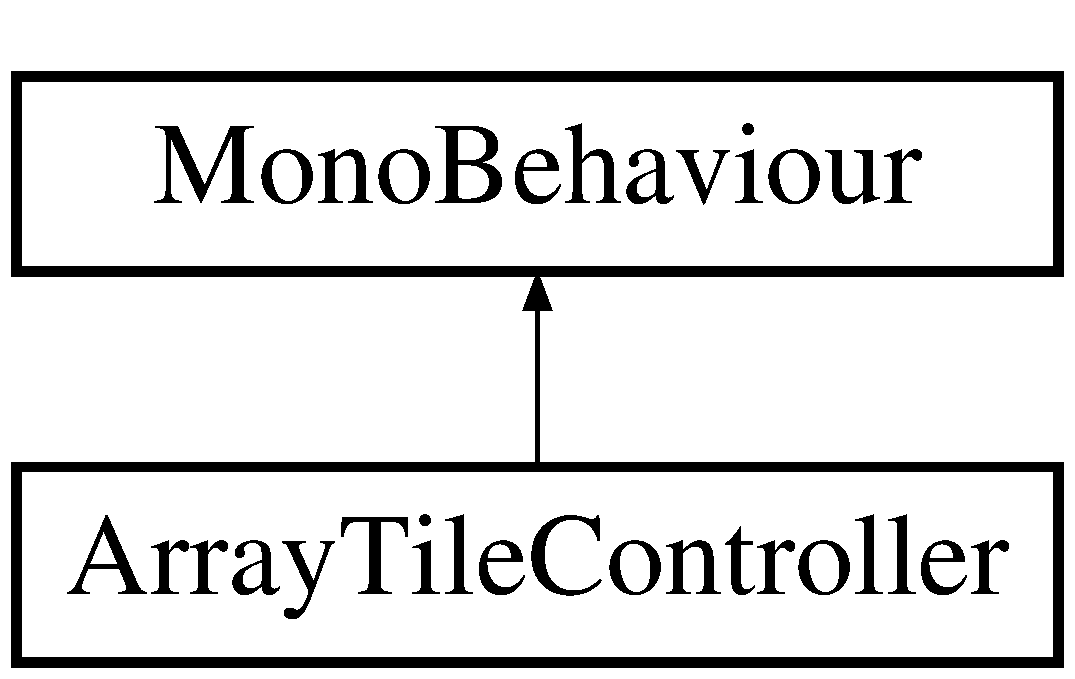
\includegraphics[height=2.000000cm]{class_array_tile_controller}
\end{center}
\end{figure}
\subsection*{Public Member Functions}
\begin{DoxyCompactItemize}
\item 
void \hyperlink{class_array_tile_controller_ab8f5d31d582f80a87d6e7ffca8dd9dce}{reset\+Used} ()
\end{DoxyCompactItemize}
\subsection*{Public Attributes}
\begin{DoxyCompactItemize}
\item 
string \hyperlink{class_array_tile_controller_a9f7d6d4fd87723a3e91209f35bc8d5f6}{tile\+Name}
\item 
\hyperlink{class_array_box_controller}{Array\+Box\+Controller} \hyperlink{class_array_tile_controller_a2ad475baebfedaf0690af41e9a243b01}{connected\+Box}
\item 
\hyperlink{class_platform_access_controller}{Platform\+Access\+Controller} \hyperlink{class_array_tile_controller_aadb469bbd5a6e7ae326b5935e50ccd8a}{connected\+Platform}
\item 
bool \hyperlink{class_array_tile_controller_a3a6ff99fac5882cc1db2be7776818e43}{is\+Used}
\end{DoxyCompactItemize}


\subsection{Detailed Description}
Manages the array Tiles Stores the tiles name,connected box(array level) Stores connected platform(array level) 

\subsection{Member Function Documentation}
\mbox{\Hypertarget{class_array_tile_controller_ab8f5d31d582f80a87d6e7ffca8dd9dce}\label{class_array_tile_controller_ab8f5d31d582f80a87d6e7ffca8dd9dce}} 
\index{Array\+Tile\+Controller@{Array\+Tile\+Controller}!reset\+Used@{reset\+Used}}
\index{reset\+Used@{reset\+Used}!Array\+Tile\+Controller@{Array\+Tile\+Controller}}
\subsubsection{\texorpdfstring{reset\+Used()}{resetUsed()}}
{\footnotesize\ttfamily void Array\+Tile\+Controller.\+reset\+Used (\begin{DoxyParamCaption}{ }\end{DoxyParamCaption})}



\subsection{Member Data Documentation}
\mbox{\Hypertarget{class_array_tile_controller_a2ad475baebfedaf0690af41e9a243b01}\label{class_array_tile_controller_a2ad475baebfedaf0690af41e9a243b01}} 
\index{Array\+Tile\+Controller@{Array\+Tile\+Controller}!connected\+Box@{connected\+Box}}
\index{connected\+Box@{connected\+Box}!Array\+Tile\+Controller@{Array\+Tile\+Controller}}
\subsubsection{\texorpdfstring{connected\+Box}{connectedBox}}
{\footnotesize\ttfamily \hyperlink{class_array_box_controller}{Array\+Box\+Controller} Array\+Tile\+Controller.\+connected\+Box}

\mbox{\Hypertarget{class_array_tile_controller_aadb469bbd5a6e7ae326b5935e50ccd8a}\label{class_array_tile_controller_aadb469bbd5a6e7ae326b5935e50ccd8a}} 
\index{Array\+Tile\+Controller@{Array\+Tile\+Controller}!connected\+Platform@{connected\+Platform}}
\index{connected\+Platform@{connected\+Platform}!Array\+Tile\+Controller@{Array\+Tile\+Controller}}
\subsubsection{\texorpdfstring{connected\+Platform}{connectedPlatform}}
{\footnotesize\ttfamily \hyperlink{class_platform_access_controller}{Platform\+Access\+Controller} Array\+Tile\+Controller.\+connected\+Platform}

\mbox{\Hypertarget{class_array_tile_controller_a3a6ff99fac5882cc1db2be7776818e43}\label{class_array_tile_controller_a3a6ff99fac5882cc1db2be7776818e43}} 
\index{Array\+Tile\+Controller@{Array\+Tile\+Controller}!is\+Used@{is\+Used}}
\index{is\+Used@{is\+Used}!Array\+Tile\+Controller@{Array\+Tile\+Controller}}
\subsubsection{\texorpdfstring{is\+Used}{isUsed}}
{\footnotesize\ttfamily bool Array\+Tile\+Controller.\+is\+Used}

\mbox{\Hypertarget{class_array_tile_controller_a9f7d6d4fd87723a3e91209f35bc8d5f6}\label{class_array_tile_controller_a9f7d6d4fd87723a3e91209f35bc8d5f6}} 
\index{Array\+Tile\+Controller@{Array\+Tile\+Controller}!tile\+Name@{tile\+Name}}
\index{tile\+Name@{tile\+Name}!Array\+Tile\+Controller@{Array\+Tile\+Controller}}
\subsubsection{\texorpdfstring{tile\+Name}{tileName}}
{\footnotesize\ttfamily string Array\+Tile\+Controller.\+tile\+Name}



The documentation for this class was generated from the following file\+:\begin{DoxyCompactItemize}
\item 
/\+Users/kwanholloway/git/5001\+Project/\+Game\+Project/\+Assets/\+Scripts/\+Puzzle\+Logic/\+Array\+Sumation\+Puzzle/\hyperlink{_array_tile_controller_8cs}{Array\+Tile\+Controller.\+cs}\end{DoxyCompactItemize}

\hypertarget{class_arr_cams_controller}{}\section{Arr\+Cams\+Controller Class Reference}
\label{class_arr_cams_controller}\index{Arr\+Cams\+Controller@{Arr\+Cams\+Controller}}
Inheritance diagram for Arr\+Cams\+Controller\+:\begin{figure}[H]
\begin{center}
\leavevmode
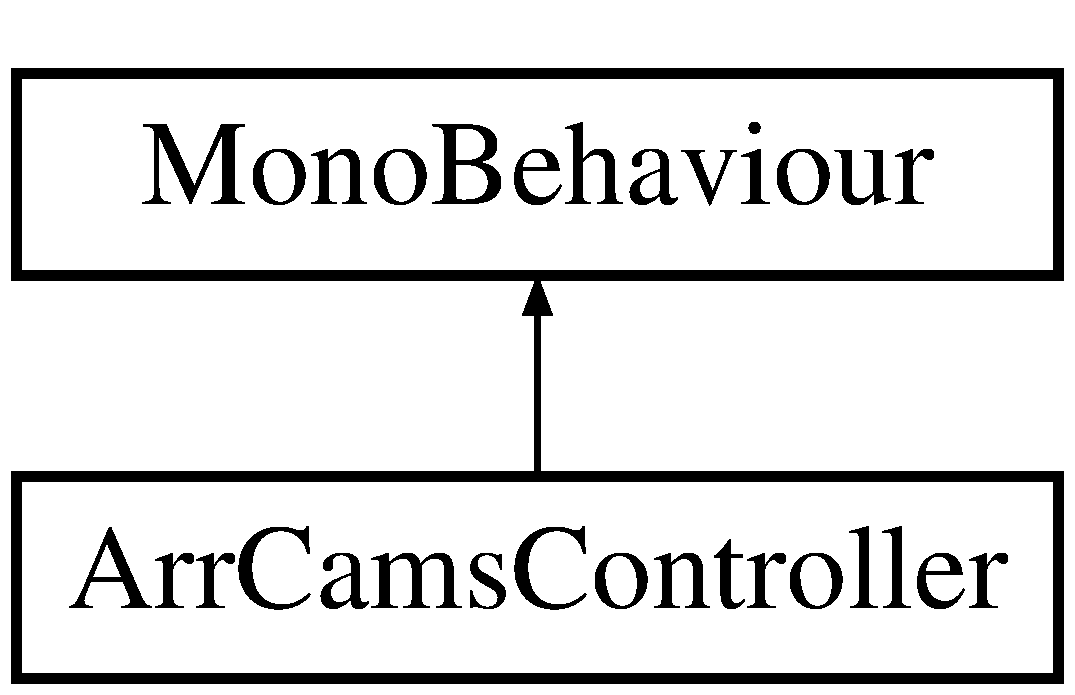
\includegraphics[height=2.000000cm]{class_arr_cams_controller}
\end{center}
\end{figure}


\subsection{Detailed Description}
Allows the player to toggle between camera that show the platforms or boxes in the array level 

The documentation for this class was generated from the following file\+:\begin{DoxyCompactItemize}
\item 
/\+Users/kwanholloway/git/5001\+Project/\+Game\+Project/\+Assets/\+Scripts/\+Game\+Logic/\hyperlink{_arr_cams_controller_8cs}{Arr\+Cams\+Controller.\+cs}\end{DoxyCompactItemize}

\hypertarget{classbomb_logic}{}\section{bomb\+Logic Class Reference}
\label{classbomb_logic}\index{bomb\+Logic@{bomb\+Logic}}
Inheritance diagram for bomb\+Logic\+:\begin{figure}[H]
\begin{center}
\leavevmode
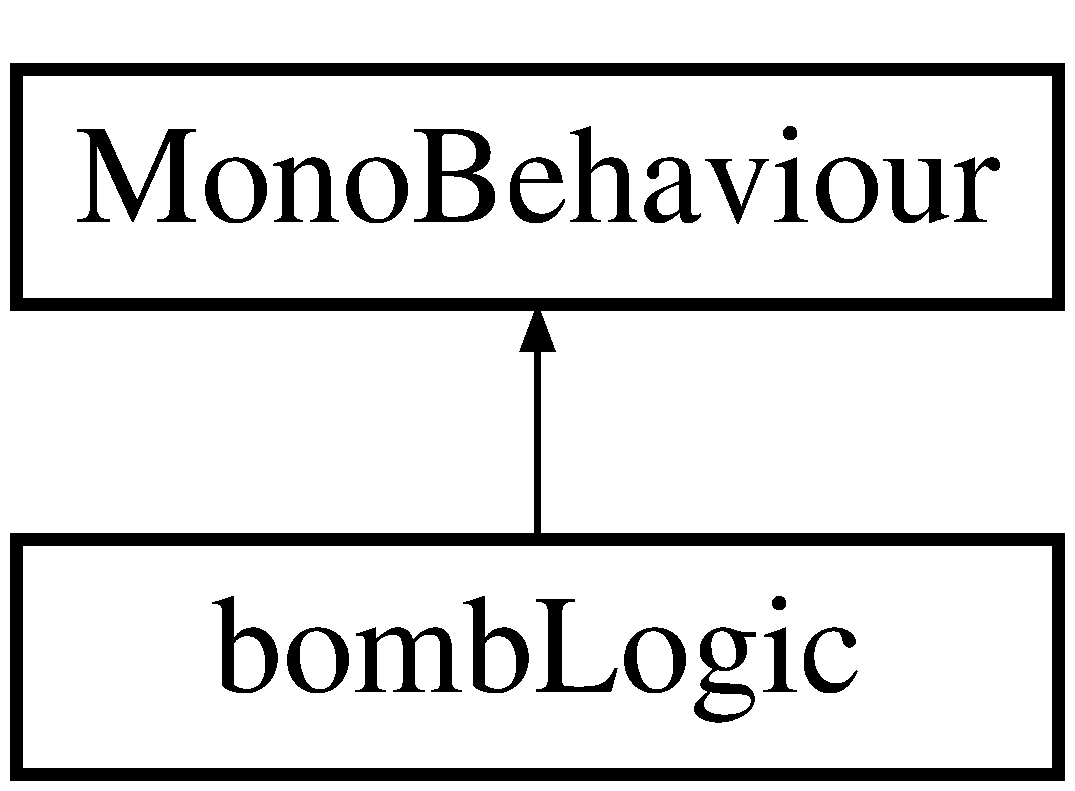
\includegraphics[height=2.000000cm]{classbomb_logic}
\end{center}
\end{figure}
\subsection*{Public Member Functions}
\begin{DoxyCompactItemize}
\item 
void \hyperlink{classbomb_logic_ae905cf9c5b66b2f88fda2c9c56ad544e}{reset\+Time} ()
\end{DoxyCompactItemize}
\subsection*{Public Attributes}
\begin{DoxyCompactItemize}
\item 
float \hyperlink{classbomb_logic_a228ae603f0d01e43eb67c2c5dea04a96}{start\+Time}
\item 
Game\+Object \hyperlink{classbomb_logic_ac6665f96ce4dd6eb83e5f3e7aff71f40}{explosion}
\end{DoxyCompactItemize}


\subsection{Member Function Documentation}
\mbox{\Hypertarget{classbomb_logic_ae905cf9c5b66b2f88fda2c9c56ad544e}\label{classbomb_logic_ae905cf9c5b66b2f88fda2c9c56ad544e}} 
\index{bomb\+Logic@{bomb\+Logic}!reset\+Time@{reset\+Time}}
\index{reset\+Time@{reset\+Time}!bomb\+Logic@{bomb\+Logic}}
\subsubsection{\texorpdfstring{reset\+Time()}{resetTime()}}
{\footnotesize\ttfamily void bomb\+Logic.\+reset\+Time (\begin{DoxyParamCaption}{ }\end{DoxyParamCaption})}



\subsection{Member Data Documentation}
\mbox{\Hypertarget{classbomb_logic_ac6665f96ce4dd6eb83e5f3e7aff71f40}\label{classbomb_logic_ac6665f96ce4dd6eb83e5f3e7aff71f40}} 
\index{bomb\+Logic@{bomb\+Logic}!explosion@{explosion}}
\index{explosion@{explosion}!bomb\+Logic@{bomb\+Logic}}
\subsubsection{\texorpdfstring{explosion}{explosion}}
{\footnotesize\ttfamily Game\+Object bomb\+Logic.\+explosion}

\mbox{\Hypertarget{classbomb_logic_a228ae603f0d01e43eb67c2c5dea04a96}\label{classbomb_logic_a228ae603f0d01e43eb67c2c5dea04a96}} 
\index{bomb\+Logic@{bomb\+Logic}!start\+Time@{start\+Time}}
\index{start\+Time@{start\+Time}!bomb\+Logic@{bomb\+Logic}}
\subsubsection{\texorpdfstring{start\+Time}{startTime}}
{\footnotesize\ttfamily float bomb\+Logic.\+start\+Time}



The documentation for this class was generated from the following file\+:\begin{DoxyCompactItemize}
\item 
/\+Users/kwanholloway/git/5001\+Project/\+Game\+Project/\+Assets/\+Scripts/\+Game\+Logic/\hyperlink{bomb_logic_8cs}{bomb\+Logic.\+cs}\end{DoxyCompactItemize}

\hypertarget{class_bool_ops_completion}{}\section{Bool\+Ops\+Completion Class Reference}
\label{class_bool_ops_completion}\index{Bool\+Ops\+Completion@{Bool\+Ops\+Completion}}
Inheritance diagram for Bool\+Ops\+Completion\+:\begin{figure}[H]
\begin{center}
\leavevmode
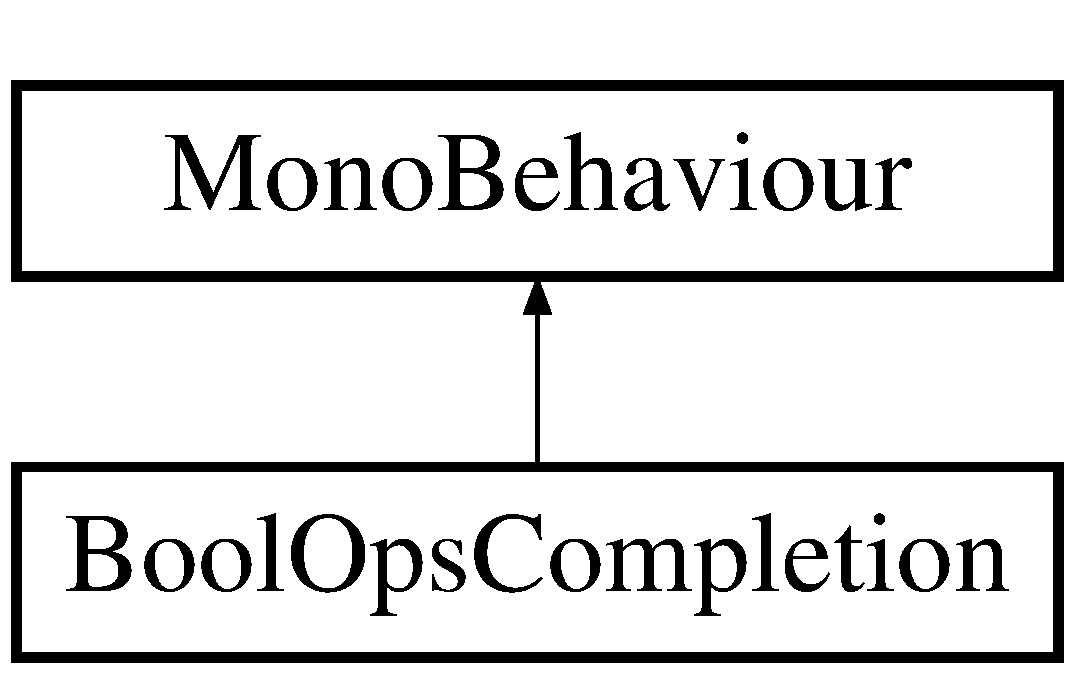
\includegraphics[height=2.000000cm]{class_bool_ops_completion}
\end{center}
\end{figure}
\subsection*{Public Member Functions}
\begin{DoxyCompactItemize}
\item 
void \hyperlink{class_bool_ops_completion_aa37088b2b4f2f10bffcfdb9accb2fde5}{reset\+Check\+Values} ()
\item 
void \hyperlink{class_bool_ops_completion_acf53c594f26e55aabd250724dc92ba53}{reset\+Puzzle} ()
\item 
void \hyperlink{class_bool_ops_completion_a6ce981e2a1853f4708ff01db8eabdcd9}{reset\+Slots} ()
\item 
void \hyperlink{class_bool_ops_completion_a665c424ab9487b5cf663921b38b86a1c}{reset\+Tiles} ()
\item 
void \hyperlink{class_bool_ops_completion_a49619737dd343ae03519ff6db1eeebc2}{reset\+Active} ()
\end{DoxyCompactItemize}
\subsection*{Public Attributes}
\begin{DoxyCompactItemize}
\item 
\hyperlink{class_array_reaction}{Array\+Reaction} \hyperlink{class_bool_ops_completion_a125b0cee3df92d1129222378c68776de}{up\+Success}
\item 
\hyperlink{class_array_reaction}{Array\+Reaction} \hyperlink{class_bool_ops_completion_a1e2dab96d55c7681be9d553f96fa652f}{replacement\+True}
\item 
\hyperlink{class_elevator_controller}{Elevator\+Controller} \hyperlink{class_bool_ops_completion_a987550dba04494bc4f310799b5f578d6}{floor\+Location}
\item 
Audio\+Source \hyperlink{class_bool_ops_completion_a1d343ac77c80d677ef0872217fcd5dc6}{solved}
\item 
bool \hyperlink{class_bool_ops_completion_a091b63eacef0cfc3a50f79e4a2e98fb2}{puzzle\+Finished}
\item 
Game\+Object \mbox{[}$\,$\mbox{]} \hyperlink{class_bool_ops_completion_a123c64568a207492685649213dd0d25f}{array\+Tiles}
\item 
Game\+Object \mbox{[}$\,$\mbox{]} \hyperlink{class_bool_ops_completion_a5c3233d04c96464e3014aa88e9c2ff37}{replacement\+Tiles}
\end{DoxyCompactItemize}


\subsection{Detailed Description}
Checks the respective challenge and makes changes to the game if the user is correct or not Challenge\+: Elevator controller in Conditional 

\subsection{Member Function Documentation}
\mbox{\Hypertarget{class_bool_ops_completion_a49619737dd343ae03519ff6db1eeebc2}\label{class_bool_ops_completion_a49619737dd343ae03519ff6db1eeebc2}} 
\index{Bool\+Ops\+Completion@{Bool\+Ops\+Completion}!reset\+Active@{reset\+Active}}
\index{reset\+Active@{reset\+Active}!Bool\+Ops\+Completion@{Bool\+Ops\+Completion}}
\subsubsection{\texorpdfstring{reset\+Active()}{resetActive()}}
{\footnotesize\ttfamily void Bool\+Ops\+Completion.\+reset\+Active (\begin{DoxyParamCaption}{ }\end{DoxyParamCaption})}

\mbox{\Hypertarget{class_bool_ops_completion_aa37088b2b4f2f10bffcfdb9accb2fde5}\label{class_bool_ops_completion_aa37088b2b4f2f10bffcfdb9accb2fde5}} 
\index{Bool\+Ops\+Completion@{Bool\+Ops\+Completion}!reset\+Check\+Values@{reset\+Check\+Values}}
\index{reset\+Check\+Values@{reset\+Check\+Values}!Bool\+Ops\+Completion@{Bool\+Ops\+Completion}}
\subsubsection{\texorpdfstring{reset\+Check\+Values()}{resetCheckValues()}}
{\footnotesize\ttfamily void Bool\+Ops\+Completion.\+reset\+Check\+Values (\begin{DoxyParamCaption}{ }\end{DoxyParamCaption})}

\mbox{\Hypertarget{class_bool_ops_completion_acf53c594f26e55aabd250724dc92ba53}\label{class_bool_ops_completion_acf53c594f26e55aabd250724dc92ba53}} 
\index{Bool\+Ops\+Completion@{Bool\+Ops\+Completion}!reset\+Puzzle@{reset\+Puzzle}}
\index{reset\+Puzzle@{reset\+Puzzle}!Bool\+Ops\+Completion@{Bool\+Ops\+Completion}}
\subsubsection{\texorpdfstring{reset\+Puzzle()}{resetPuzzle()}}
{\footnotesize\ttfamily void Bool\+Ops\+Completion.\+reset\+Puzzle (\begin{DoxyParamCaption}{ }\end{DoxyParamCaption})}

\mbox{\Hypertarget{class_bool_ops_completion_a6ce981e2a1853f4708ff01db8eabdcd9}\label{class_bool_ops_completion_a6ce981e2a1853f4708ff01db8eabdcd9}} 
\index{Bool\+Ops\+Completion@{Bool\+Ops\+Completion}!reset\+Slots@{reset\+Slots}}
\index{reset\+Slots@{reset\+Slots}!Bool\+Ops\+Completion@{Bool\+Ops\+Completion}}
\subsubsection{\texorpdfstring{reset\+Slots()}{resetSlots()}}
{\footnotesize\ttfamily void Bool\+Ops\+Completion.\+reset\+Slots (\begin{DoxyParamCaption}{ }\end{DoxyParamCaption})}

\mbox{\Hypertarget{class_bool_ops_completion_a665c424ab9487b5cf663921b38b86a1c}\label{class_bool_ops_completion_a665c424ab9487b5cf663921b38b86a1c}} 
\index{Bool\+Ops\+Completion@{Bool\+Ops\+Completion}!reset\+Tiles@{reset\+Tiles}}
\index{reset\+Tiles@{reset\+Tiles}!Bool\+Ops\+Completion@{Bool\+Ops\+Completion}}
\subsubsection{\texorpdfstring{reset\+Tiles()}{resetTiles()}}
{\footnotesize\ttfamily void Bool\+Ops\+Completion.\+reset\+Tiles (\begin{DoxyParamCaption}{ }\end{DoxyParamCaption})}



\subsection{Member Data Documentation}
\mbox{\Hypertarget{class_bool_ops_completion_a123c64568a207492685649213dd0d25f}\label{class_bool_ops_completion_a123c64568a207492685649213dd0d25f}} 
\index{Bool\+Ops\+Completion@{Bool\+Ops\+Completion}!array\+Tiles@{array\+Tiles}}
\index{array\+Tiles@{array\+Tiles}!Bool\+Ops\+Completion@{Bool\+Ops\+Completion}}
\subsubsection{\texorpdfstring{array\+Tiles}{arrayTiles}}
{\footnotesize\ttfamily Game\+Object \mbox{[}$\,$\mbox{]} Bool\+Ops\+Completion.\+array\+Tiles}

\mbox{\Hypertarget{class_bool_ops_completion_a987550dba04494bc4f310799b5f578d6}\label{class_bool_ops_completion_a987550dba04494bc4f310799b5f578d6}} 
\index{Bool\+Ops\+Completion@{Bool\+Ops\+Completion}!floor\+Location@{floor\+Location}}
\index{floor\+Location@{floor\+Location}!Bool\+Ops\+Completion@{Bool\+Ops\+Completion}}
\subsubsection{\texorpdfstring{floor\+Location}{floorLocation}}
{\footnotesize\ttfamily \hyperlink{class_elevator_controller}{Elevator\+Controller} Bool\+Ops\+Completion.\+floor\+Location}

\mbox{\Hypertarget{class_bool_ops_completion_a091b63eacef0cfc3a50f79e4a2e98fb2}\label{class_bool_ops_completion_a091b63eacef0cfc3a50f79e4a2e98fb2}} 
\index{Bool\+Ops\+Completion@{Bool\+Ops\+Completion}!puzzle\+Finished@{puzzle\+Finished}}
\index{puzzle\+Finished@{puzzle\+Finished}!Bool\+Ops\+Completion@{Bool\+Ops\+Completion}}
\subsubsection{\texorpdfstring{puzzle\+Finished}{puzzleFinished}}
{\footnotesize\ttfamily bool Bool\+Ops\+Completion.\+puzzle\+Finished}

\mbox{\Hypertarget{class_bool_ops_completion_a5c3233d04c96464e3014aa88e9c2ff37}\label{class_bool_ops_completion_a5c3233d04c96464e3014aa88e9c2ff37}} 
\index{Bool\+Ops\+Completion@{Bool\+Ops\+Completion}!replacement\+Tiles@{replacement\+Tiles}}
\index{replacement\+Tiles@{replacement\+Tiles}!Bool\+Ops\+Completion@{Bool\+Ops\+Completion}}
\subsubsection{\texorpdfstring{replacement\+Tiles}{replacementTiles}}
{\footnotesize\ttfamily Game\+Object \mbox{[}$\,$\mbox{]} Bool\+Ops\+Completion.\+replacement\+Tiles}

\mbox{\Hypertarget{class_bool_ops_completion_a1e2dab96d55c7681be9d553f96fa652f}\label{class_bool_ops_completion_a1e2dab96d55c7681be9d553f96fa652f}} 
\index{Bool\+Ops\+Completion@{Bool\+Ops\+Completion}!replacement\+True@{replacement\+True}}
\index{replacement\+True@{replacement\+True}!Bool\+Ops\+Completion@{Bool\+Ops\+Completion}}
\subsubsection{\texorpdfstring{replacement\+True}{replacementTrue}}
{\footnotesize\ttfamily \hyperlink{class_array_reaction}{Array\+Reaction} Bool\+Ops\+Completion.\+replacement\+True}

\mbox{\Hypertarget{class_bool_ops_completion_a1d343ac77c80d677ef0872217fcd5dc6}\label{class_bool_ops_completion_a1d343ac77c80d677ef0872217fcd5dc6}} 
\index{Bool\+Ops\+Completion@{Bool\+Ops\+Completion}!solved@{solved}}
\index{solved@{solved}!Bool\+Ops\+Completion@{Bool\+Ops\+Completion}}
\subsubsection{\texorpdfstring{solved}{solved}}
{\footnotesize\ttfamily Audio\+Source Bool\+Ops\+Completion.\+solved}

\mbox{\Hypertarget{class_bool_ops_completion_a125b0cee3df92d1129222378c68776de}\label{class_bool_ops_completion_a125b0cee3df92d1129222378c68776de}} 
\index{Bool\+Ops\+Completion@{Bool\+Ops\+Completion}!up\+Success@{up\+Success}}
\index{up\+Success@{up\+Success}!Bool\+Ops\+Completion@{Bool\+Ops\+Completion}}
\subsubsection{\texorpdfstring{up\+Success}{upSuccess}}
{\footnotesize\ttfamily \hyperlink{class_array_reaction}{Array\+Reaction} Bool\+Ops\+Completion.\+up\+Success}



The documentation for this class was generated from the following file\+:\begin{DoxyCompactItemize}
\item 
/\+Users/kwanholloway/git/5001\+Project/\+Game\+Project/\+Assets/\+Scripts/\+Puzzle\+Logic/\+Conditional Level/\hyperlink{_bool_ops_completion_8cs}{Bool\+Ops\+Completion.\+cs}\end{DoxyCompactItemize}

\hypertarget{class_camera_follow}{}\section{Camera\+Follow Class Reference}
\label{class_camera_follow}\index{Camera\+Follow@{Camera\+Follow}}
Inheritance diagram for Camera\+Follow\+:\begin{figure}[H]
\begin{center}
\leavevmode
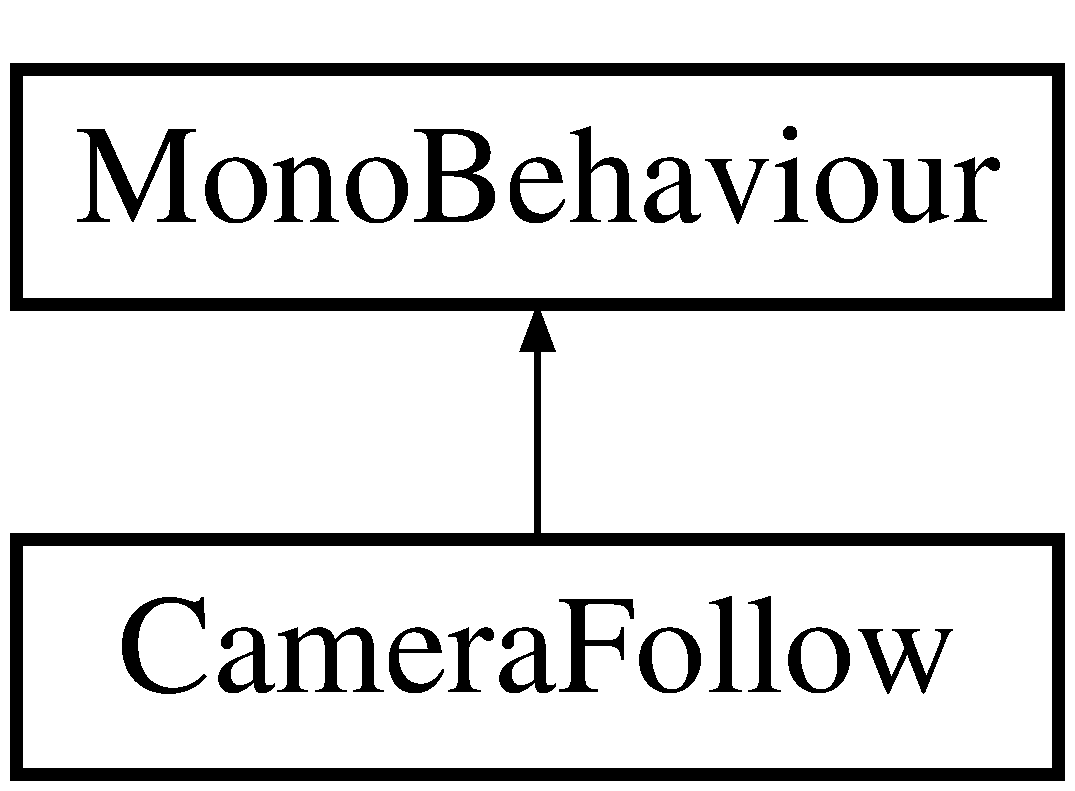
\includegraphics[height=2.000000cm]{class_camera_follow}
\end{center}
\end{figure}
\subsection*{Public Attributes}
\begin{DoxyCompactItemize}
\item 
float \hyperlink{class_camera_follow_a1bc45f6500779db9197b6620308a3589}{camera\+Speed}
\end{DoxyCompactItemize}


\subsection{Detailed Description}
Manages the camera and allows it to follow the player 

\subsection{Member Data Documentation}
\mbox{\Hypertarget{class_camera_follow_a1bc45f6500779db9197b6620308a3589}\label{class_camera_follow_a1bc45f6500779db9197b6620308a3589}} 
\index{Camera\+Follow@{Camera\+Follow}!camera\+Speed@{camera\+Speed}}
\index{camera\+Speed@{camera\+Speed}!Camera\+Follow@{Camera\+Follow}}
\subsubsection{\texorpdfstring{camera\+Speed}{cameraSpeed}}
{\footnotesize\ttfamily float Camera\+Follow.\+camera\+Speed}



The documentation for this class was generated from the following file\+:\begin{DoxyCompactItemize}
\item 
/\+Users/kwanholloway/git/5001\+Project/\+Game\+Project/\+Assets/\+Scripts/\+Player/\hyperlink{_camera_follow_8cs}{Camera\+Follow.\+cs}\end{DoxyCompactItemize}

\hypertarget{classcamera_zoom}{}\section{camera\+Zoom Class Reference}
\label{classcamera_zoom}\index{camera\+Zoom@{camera\+Zoom}}
Inheritance diagram for camera\+Zoom\+:\begin{figure}[H]
\begin{center}
\leavevmode
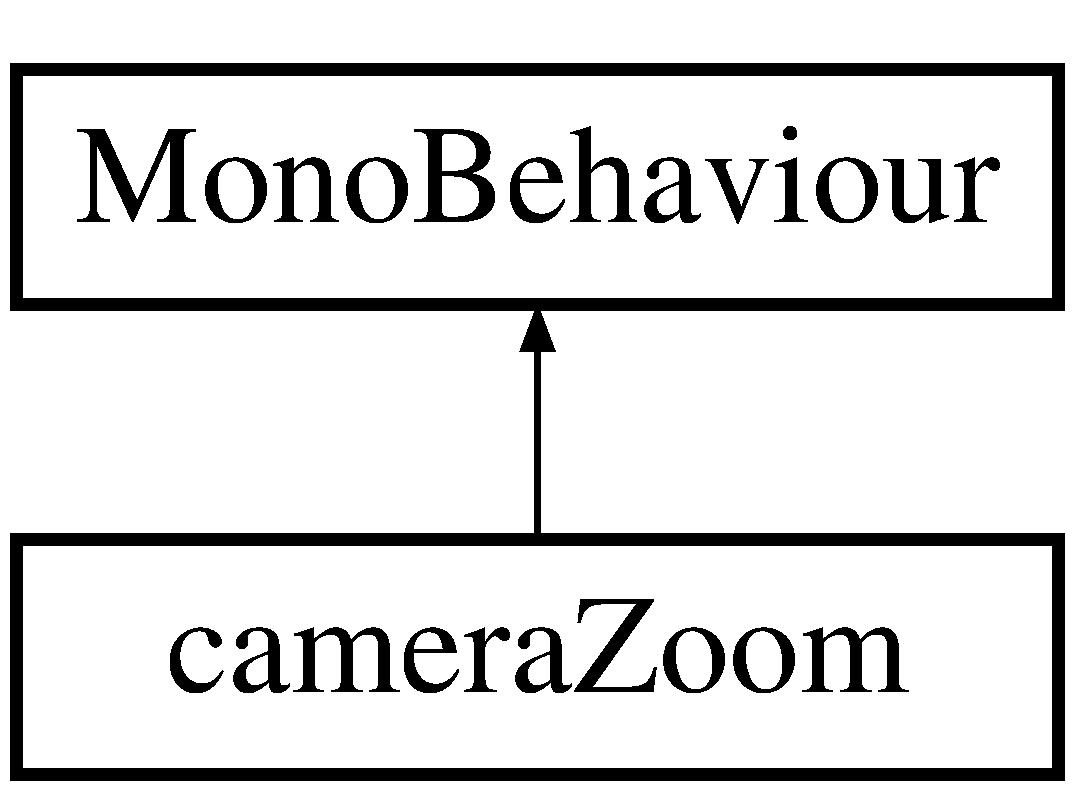
\includegraphics[height=2.000000cm]{classcamera_zoom}
\end{center}
\end{figure}
\subsection*{Public Attributes}
\begin{DoxyCompactItemize}
\item 
Camera \hyperlink{classcamera_zoom_ac4110b23099c06c7c7d23a41200802bd}{this\+Camera}
\item 
bool \hyperlink{classcamera_zoom_a808d6a51143de0d2af012b993f972b0f}{in\+Area}
\end{DoxyCompactItemize}


\subsection{Member Data Documentation}
\mbox{\Hypertarget{classcamera_zoom_a808d6a51143de0d2af012b993f972b0f}\label{classcamera_zoom_a808d6a51143de0d2af012b993f972b0f}} 
\index{camera\+Zoom@{camera\+Zoom}!in\+Area@{in\+Area}}
\index{in\+Area@{in\+Area}!camera\+Zoom@{camera\+Zoom}}
\subsubsection{\texorpdfstring{in\+Area}{inArea}}
{\footnotesize\ttfamily bool camera\+Zoom.\+in\+Area}

\mbox{\Hypertarget{classcamera_zoom_ac4110b23099c06c7c7d23a41200802bd}\label{classcamera_zoom_ac4110b23099c06c7c7d23a41200802bd}} 
\index{camera\+Zoom@{camera\+Zoom}!this\+Camera@{this\+Camera}}
\index{this\+Camera@{this\+Camera}!camera\+Zoom@{camera\+Zoom}}
\subsubsection{\texorpdfstring{this\+Camera}{thisCamera}}
{\footnotesize\ttfamily Camera camera\+Zoom.\+this\+Camera}



The documentation for this class was generated from the following file\+:\begin{DoxyCompactItemize}
\item 
/\+Users/kwanholloway/git/5001\+Project/\+Game\+Project/\+Assets/\+Scripts/\+Z-\/\+N\+O\+T U\+S\+E\+D/\hyperlink{camera_zoom_8cs}{camera\+Zoom.\+cs}\end{DoxyCompactItemize}

\hypertarget{class_completion_check}{}\section{Completion\+Check Class Reference}
\label{class_completion_check}\index{Completion\+Check@{Completion\+Check}}
Inheritance diagram for Completion\+Check\+:\begin{figure}[H]
\begin{center}
\leavevmode
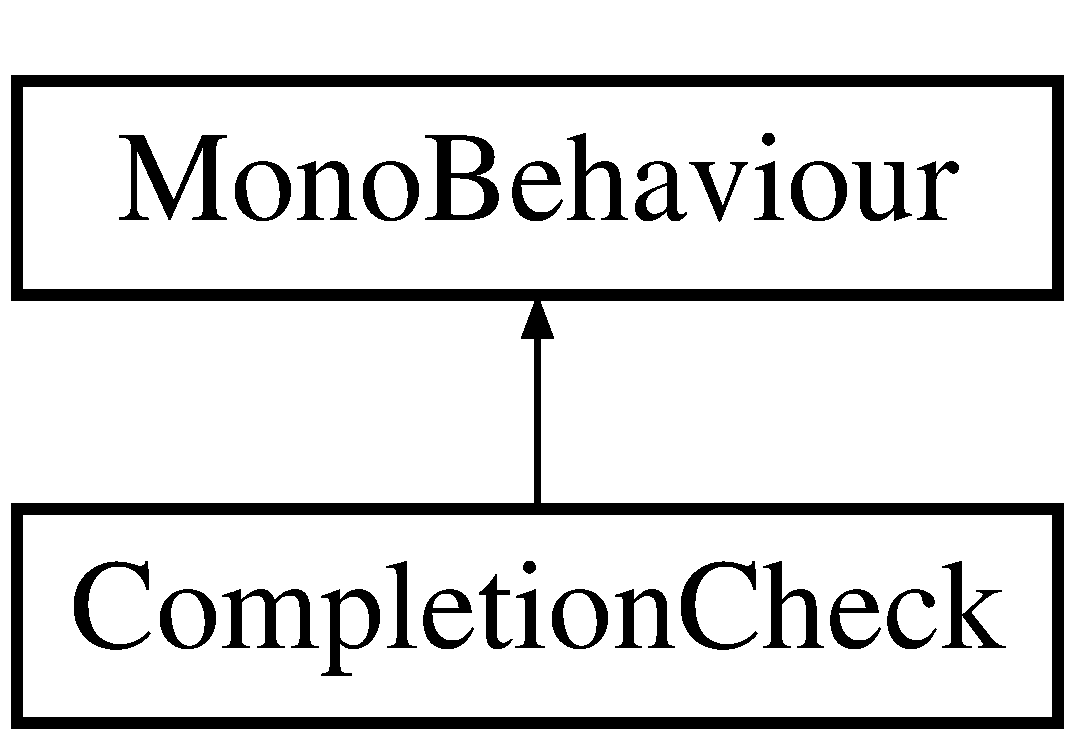
\includegraphics[height=2.000000cm]{class_completion_check}
\end{center}
\end{figure}
\subsection*{Public Member Functions}
\begin{DoxyCompactItemize}
\item 
void \hyperlink{class_completion_check_a98191957075533d151dc7698427e60ef}{reset\+Puzzle} ()
\item 
void \hyperlink{class_completion_check_aca7af54ed862a4e68ea33ba918552526}{reset\+Check\+Values} ()
\item 
void \hyperlink{class_completion_check_ad8abae4b94bcebbbc02baa666f7edba1}{reset\+Slots} ()
\item 
void \hyperlink{class_completion_check_a728598fbba43df4fda2542630af671ee}{reset\+Tiles} ()
\item 
void \hyperlink{class_completion_check_a54ea0b1dfecf4892ff9f43b0399c4dda}{reset\+Active} ()
\end{DoxyCompactItemize}
\subsection*{Public Attributes}
\begin{DoxyCompactItemize}
\item 
\hyperlink{class_array_reaction}{Array\+Reaction} \hyperlink{class_completion_check_a565266c6464718da6c52d813c3b0ff32}{two\+Success}
\item 
\hyperlink{class_array_reaction}{Array\+Reaction} \hyperlink{class_completion_check_ab2384403c14606be2c726ba3fb4278f2}{replacement\+Two}
\item 
\hyperlink{class_array_reaction}{Array\+Reaction} \hyperlink{class_completion_check_ac92b5dad9a4e4aee625e20fce2fb4d0f}{replacement\+Plus}
\item 
\hyperlink{class_array_reaction}{Array\+Reaction} \hyperlink{class_completion_check_a90ecb0589046ab6ecc5a00bec9c266c0}{replacement\+Plus\+Plus}
\item 
Audio\+Source \hyperlink{class_completion_check_ab3aee64fe90f53bb4cff27b659072472}{solved}
\item 
bool \hyperlink{class_completion_check_a1b78317104756d1316af22e2bb555e4a}{puzzle\+Finished}
\item 
Game\+Object \hyperlink{class_completion_check_ae9a5f29e14ffbe992a16f08ebc2dc9f4}{door\+One}
\item 
Game\+Object \mbox{[}$\,$\mbox{]} \hyperlink{class_completion_check_ad53ac3b7c0d769b85b53bdb222172b7d}{array\+Tiles}
\item 
Game\+Object \mbox{[}$\,$\mbox{]} \hyperlink{class_completion_check_a2a5b3a10802d72c018ddc7f1d41ae60c}{replacement\+Tiles}
\end{DoxyCompactItemize}


\subsection{Detailed Description}
Checks the respective challenge and makes changes to the game if the user is correct or not Challenge\+: Loop challenge 1 

\subsection{Member Function Documentation}
\mbox{\Hypertarget{class_completion_check_a54ea0b1dfecf4892ff9f43b0399c4dda}\label{class_completion_check_a54ea0b1dfecf4892ff9f43b0399c4dda}} 
\index{Completion\+Check@{Completion\+Check}!reset\+Active@{reset\+Active}}
\index{reset\+Active@{reset\+Active}!Completion\+Check@{Completion\+Check}}
\subsubsection{\texorpdfstring{reset\+Active()}{resetActive()}}
{\footnotesize\ttfamily void Completion\+Check.\+reset\+Active (\begin{DoxyParamCaption}{ }\end{DoxyParamCaption})}

\mbox{\Hypertarget{class_completion_check_aca7af54ed862a4e68ea33ba918552526}\label{class_completion_check_aca7af54ed862a4e68ea33ba918552526}} 
\index{Completion\+Check@{Completion\+Check}!reset\+Check\+Values@{reset\+Check\+Values}}
\index{reset\+Check\+Values@{reset\+Check\+Values}!Completion\+Check@{Completion\+Check}}
\subsubsection{\texorpdfstring{reset\+Check\+Values()}{resetCheckValues()}}
{\footnotesize\ttfamily void Completion\+Check.\+reset\+Check\+Values (\begin{DoxyParamCaption}{ }\end{DoxyParamCaption})}

\mbox{\Hypertarget{class_completion_check_a98191957075533d151dc7698427e60ef}\label{class_completion_check_a98191957075533d151dc7698427e60ef}} 
\index{Completion\+Check@{Completion\+Check}!reset\+Puzzle@{reset\+Puzzle}}
\index{reset\+Puzzle@{reset\+Puzzle}!Completion\+Check@{Completion\+Check}}
\subsubsection{\texorpdfstring{reset\+Puzzle()}{resetPuzzle()}}
{\footnotesize\ttfamily void Completion\+Check.\+reset\+Puzzle (\begin{DoxyParamCaption}{ }\end{DoxyParamCaption})}

\mbox{\Hypertarget{class_completion_check_ad8abae4b94bcebbbc02baa666f7edba1}\label{class_completion_check_ad8abae4b94bcebbbc02baa666f7edba1}} 
\index{Completion\+Check@{Completion\+Check}!reset\+Slots@{reset\+Slots}}
\index{reset\+Slots@{reset\+Slots}!Completion\+Check@{Completion\+Check}}
\subsubsection{\texorpdfstring{reset\+Slots()}{resetSlots()}}
{\footnotesize\ttfamily void Completion\+Check.\+reset\+Slots (\begin{DoxyParamCaption}{ }\end{DoxyParamCaption})}

\mbox{\Hypertarget{class_completion_check_a728598fbba43df4fda2542630af671ee}\label{class_completion_check_a728598fbba43df4fda2542630af671ee}} 
\index{Completion\+Check@{Completion\+Check}!reset\+Tiles@{reset\+Tiles}}
\index{reset\+Tiles@{reset\+Tiles}!Completion\+Check@{Completion\+Check}}
\subsubsection{\texorpdfstring{reset\+Tiles()}{resetTiles()}}
{\footnotesize\ttfamily void Completion\+Check.\+reset\+Tiles (\begin{DoxyParamCaption}{ }\end{DoxyParamCaption})}



\subsection{Member Data Documentation}
\mbox{\Hypertarget{class_completion_check_ad53ac3b7c0d769b85b53bdb222172b7d}\label{class_completion_check_ad53ac3b7c0d769b85b53bdb222172b7d}} 
\index{Completion\+Check@{Completion\+Check}!array\+Tiles@{array\+Tiles}}
\index{array\+Tiles@{array\+Tiles}!Completion\+Check@{Completion\+Check}}
\subsubsection{\texorpdfstring{array\+Tiles}{arrayTiles}}
{\footnotesize\ttfamily Game\+Object \mbox{[}$\,$\mbox{]} Completion\+Check.\+array\+Tiles}

\mbox{\Hypertarget{class_completion_check_ae9a5f29e14ffbe992a16f08ebc2dc9f4}\label{class_completion_check_ae9a5f29e14ffbe992a16f08ebc2dc9f4}} 
\index{Completion\+Check@{Completion\+Check}!door\+One@{door\+One}}
\index{door\+One@{door\+One}!Completion\+Check@{Completion\+Check}}
\subsubsection{\texorpdfstring{door\+One}{doorOne}}
{\footnotesize\ttfamily Game\+Object Completion\+Check.\+door\+One}

\mbox{\Hypertarget{class_completion_check_a1b78317104756d1316af22e2bb555e4a}\label{class_completion_check_a1b78317104756d1316af22e2bb555e4a}} 
\index{Completion\+Check@{Completion\+Check}!puzzle\+Finished@{puzzle\+Finished}}
\index{puzzle\+Finished@{puzzle\+Finished}!Completion\+Check@{Completion\+Check}}
\subsubsection{\texorpdfstring{puzzle\+Finished}{puzzleFinished}}
{\footnotesize\ttfamily bool Completion\+Check.\+puzzle\+Finished}

\mbox{\Hypertarget{class_completion_check_ac92b5dad9a4e4aee625e20fce2fb4d0f}\label{class_completion_check_ac92b5dad9a4e4aee625e20fce2fb4d0f}} 
\index{Completion\+Check@{Completion\+Check}!replacement\+Plus@{replacement\+Plus}}
\index{replacement\+Plus@{replacement\+Plus}!Completion\+Check@{Completion\+Check}}
\subsubsection{\texorpdfstring{replacement\+Plus}{replacementPlus}}
{\footnotesize\ttfamily \hyperlink{class_array_reaction}{Array\+Reaction} Completion\+Check.\+replacement\+Plus}

\mbox{\Hypertarget{class_completion_check_a90ecb0589046ab6ecc5a00bec9c266c0}\label{class_completion_check_a90ecb0589046ab6ecc5a00bec9c266c0}} 
\index{Completion\+Check@{Completion\+Check}!replacement\+Plus\+Plus@{replacement\+Plus\+Plus}}
\index{replacement\+Plus\+Plus@{replacement\+Plus\+Plus}!Completion\+Check@{Completion\+Check}}
\subsubsection{\texorpdfstring{replacement\+Plus\+Plus}{replacementPlusPlus}}
{\footnotesize\ttfamily \hyperlink{class_array_reaction}{Array\+Reaction} Completion\+Check.\+replacement\+Plus\+Plus}

\mbox{\Hypertarget{class_completion_check_a2a5b3a10802d72c018ddc7f1d41ae60c}\label{class_completion_check_a2a5b3a10802d72c018ddc7f1d41ae60c}} 
\index{Completion\+Check@{Completion\+Check}!replacement\+Tiles@{replacement\+Tiles}}
\index{replacement\+Tiles@{replacement\+Tiles}!Completion\+Check@{Completion\+Check}}
\subsubsection{\texorpdfstring{replacement\+Tiles}{replacementTiles}}
{\footnotesize\ttfamily Game\+Object \mbox{[}$\,$\mbox{]} Completion\+Check.\+replacement\+Tiles}

\mbox{\Hypertarget{class_completion_check_ab2384403c14606be2c726ba3fb4278f2}\label{class_completion_check_ab2384403c14606be2c726ba3fb4278f2}} 
\index{Completion\+Check@{Completion\+Check}!replacement\+Two@{replacement\+Two}}
\index{replacement\+Two@{replacement\+Two}!Completion\+Check@{Completion\+Check}}
\subsubsection{\texorpdfstring{replacement\+Two}{replacementTwo}}
{\footnotesize\ttfamily \hyperlink{class_array_reaction}{Array\+Reaction} Completion\+Check.\+replacement\+Two}

\mbox{\Hypertarget{class_completion_check_ab3aee64fe90f53bb4cff27b659072472}\label{class_completion_check_ab3aee64fe90f53bb4cff27b659072472}} 
\index{Completion\+Check@{Completion\+Check}!solved@{solved}}
\index{solved@{solved}!Completion\+Check@{Completion\+Check}}
\subsubsection{\texorpdfstring{solved}{solved}}
{\footnotesize\ttfamily Audio\+Source Completion\+Check.\+solved}

\mbox{\Hypertarget{class_completion_check_a565266c6464718da6c52d813c3b0ff32}\label{class_completion_check_a565266c6464718da6c52d813c3b0ff32}} 
\index{Completion\+Check@{Completion\+Check}!two\+Success@{two\+Success}}
\index{two\+Success@{two\+Success}!Completion\+Check@{Completion\+Check}}
\subsubsection{\texorpdfstring{two\+Success}{twoSuccess}}
{\footnotesize\ttfamily \hyperlink{class_array_reaction}{Array\+Reaction} Completion\+Check.\+two\+Success}



The documentation for this class was generated from the following file\+:\begin{DoxyCompactItemize}
\item 
/\+Users/kwanholloway/git/5001\+Project/\+Game\+Project/\+Assets/\+Scripts/\+Puzzle\+Logic/\+Loop\+Level/\+For\+Loop\+Puzzle/\hyperlink{_completion_check_8cs}{Completion\+Check.\+cs}\end{DoxyCompactItemize}

\hypertarget{class_completion_check2}{}\section{Completion\+Check2 Class Reference}
\label{class_completion_check2}\index{Completion\+Check2@{Completion\+Check2}}
Inheritance diagram for Completion\+Check2\+:\begin{figure}[H]
\begin{center}
\leavevmode
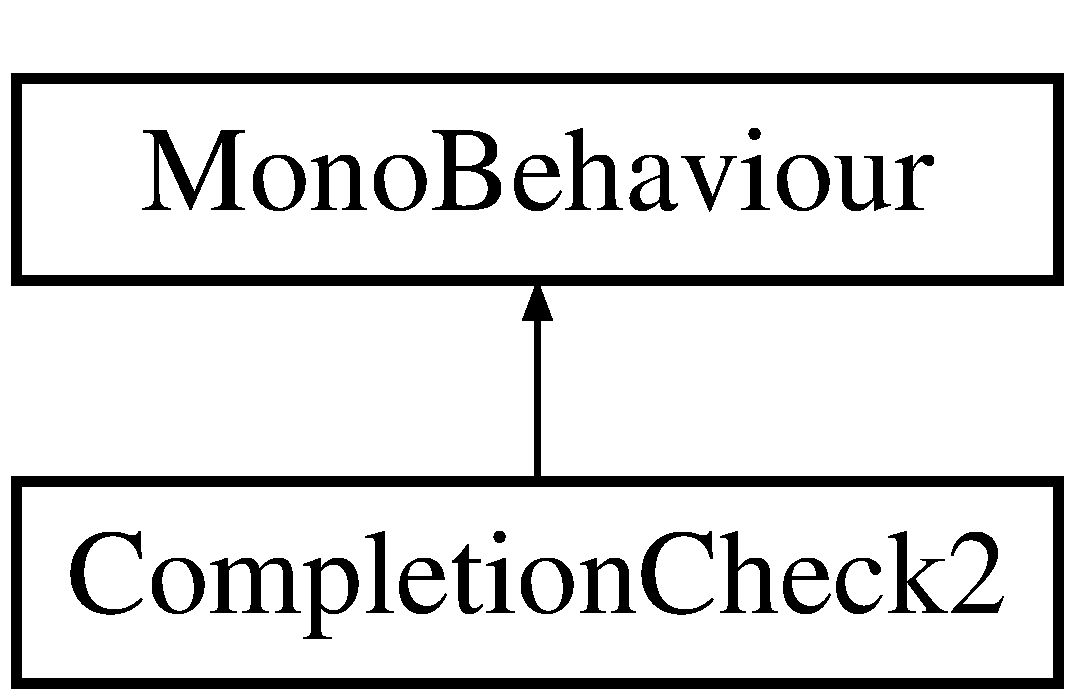
\includegraphics[height=2.000000cm]{class_completion_check2}
\end{center}
\end{figure}
\subsection*{Public Member Functions}
\begin{DoxyCompactItemize}
\item 
void \hyperlink{class_completion_check2_aa06cef9b95d2f9c4bbb498f6c9efac1e}{reset\+Puzzle} ()
\item 
void \hyperlink{class_completion_check2_ad02e4fa74bc9dfaf00961746a68d7061}{reset\+Check\+Values} ()
\item 
void \hyperlink{class_completion_check2_a35ed56dc84b27430bdacabc119985ec5}{reset\+Slots} ()
\item 
void \hyperlink{class_completion_check2_a16a374ffbff900932f113dad066d27e4}{reset\+Tiles} ()
\item 
void \hyperlink{class_completion_check2_acc81070efa47ed19e94287be80bba5da}{reset\+Active} ()
\end{DoxyCompactItemize}
\subsection*{Public Attributes}
\begin{DoxyCompactItemize}
\item 
\hyperlink{class_array_reaction}{Array\+Reaction} \hyperlink{class_completion_check2_a5304ab78c9a420165fa605e25ac5bdd6}{three\+Success}
\item 
\hyperlink{class_array_reaction}{Array\+Reaction} \hyperlink{class_completion_check2_a56390eb4e63df9107df6f1dbe6b36c34}{replacement\+Three}
\item 
bool \hyperlink{class_completion_check2_a88f888fbd3883fe7c46c6377aedd389d}{puzzle\+Finished}
\item 
Game\+Object \hyperlink{class_completion_check2_a8e504c1480b264be827cce35f4006d7e}{door\+Two}
\item 
Game\+Object \mbox{[}$\,$\mbox{]} \hyperlink{class_completion_check2_a3e576206fcbe2ffdc58b6538b10c57d2}{array\+Tiles}
\item 
Game\+Object \mbox{[}$\,$\mbox{]} \hyperlink{class_completion_check2_a712fc392f7a484070dea22d804bf0ce9}{replacement\+Tiles}
\item 
Audio\+Source \hyperlink{class_completion_check2_ab543e719625d9de2a48b6817c41c3432}{solved}
\end{DoxyCompactItemize}


\subsection{Detailed Description}
Checks the respective challenge and makes changes to the game if the user is correct or not Challenge\+: Loop challenge 3 

\subsection{Member Function Documentation}
\mbox{\Hypertarget{class_completion_check2_acc81070efa47ed19e94287be80bba5da}\label{class_completion_check2_acc81070efa47ed19e94287be80bba5da}} 
\index{Completion\+Check2@{Completion\+Check2}!reset\+Active@{reset\+Active}}
\index{reset\+Active@{reset\+Active}!Completion\+Check2@{Completion\+Check2}}
\subsubsection{\texorpdfstring{reset\+Active()}{resetActive()}}
{\footnotesize\ttfamily void Completion\+Check2.\+reset\+Active (\begin{DoxyParamCaption}{ }\end{DoxyParamCaption})}

\mbox{\Hypertarget{class_completion_check2_ad02e4fa74bc9dfaf00961746a68d7061}\label{class_completion_check2_ad02e4fa74bc9dfaf00961746a68d7061}} 
\index{Completion\+Check2@{Completion\+Check2}!reset\+Check\+Values@{reset\+Check\+Values}}
\index{reset\+Check\+Values@{reset\+Check\+Values}!Completion\+Check2@{Completion\+Check2}}
\subsubsection{\texorpdfstring{reset\+Check\+Values()}{resetCheckValues()}}
{\footnotesize\ttfamily void Completion\+Check2.\+reset\+Check\+Values (\begin{DoxyParamCaption}{ }\end{DoxyParamCaption})}

\mbox{\Hypertarget{class_completion_check2_aa06cef9b95d2f9c4bbb498f6c9efac1e}\label{class_completion_check2_aa06cef9b95d2f9c4bbb498f6c9efac1e}} 
\index{Completion\+Check2@{Completion\+Check2}!reset\+Puzzle@{reset\+Puzzle}}
\index{reset\+Puzzle@{reset\+Puzzle}!Completion\+Check2@{Completion\+Check2}}
\subsubsection{\texorpdfstring{reset\+Puzzle()}{resetPuzzle()}}
{\footnotesize\ttfamily void Completion\+Check2.\+reset\+Puzzle (\begin{DoxyParamCaption}{ }\end{DoxyParamCaption})}

\mbox{\Hypertarget{class_completion_check2_a35ed56dc84b27430bdacabc119985ec5}\label{class_completion_check2_a35ed56dc84b27430bdacabc119985ec5}} 
\index{Completion\+Check2@{Completion\+Check2}!reset\+Slots@{reset\+Slots}}
\index{reset\+Slots@{reset\+Slots}!Completion\+Check2@{Completion\+Check2}}
\subsubsection{\texorpdfstring{reset\+Slots()}{resetSlots()}}
{\footnotesize\ttfamily void Completion\+Check2.\+reset\+Slots (\begin{DoxyParamCaption}{ }\end{DoxyParamCaption})}

\mbox{\Hypertarget{class_completion_check2_a16a374ffbff900932f113dad066d27e4}\label{class_completion_check2_a16a374ffbff900932f113dad066d27e4}} 
\index{Completion\+Check2@{Completion\+Check2}!reset\+Tiles@{reset\+Tiles}}
\index{reset\+Tiles@{reset\+Tiles}!Completion\+Check2@{Completion\+Check2}}
\subsubsection{\texorpdfstring{reset\+Tiles()}{resetTiles()}}
{\footnotesize\ttfamily void Completion\+Check2.\+reset\+Tiles (\begin{DoxyParamCaption}{ }\end{DoxyParamCaption})}



\subsection{Member Data Documentation}
\mbox{\Hypertarget{class_completion_check2_a3e576206fcbe2ffdc58b6538b10c57d2}\label{class_completion_check2_a3e576206fcbe2ffdc58b6538b10c57d2}} 
\index{Completion\+Check2@{Completion\+Check2}!array\+Tiles@{array\+Tiles}}
\index{array\+Tiles@{array\+Tiles}!Completion\+Check2@{Completion\+Check2}}
\subsubsection{\texorpdfstring{array\+Tiles}{arrayTiles}}
{\footnotesize\ttfamily Game\+Object \mbox{[}$\,$\mbox{]} Completion\+Check2.\+array\+Tiles}

\mbox{\Hypertarget{class_completion_check2_a8e504c1480b264be827cce35f4006d7e}\label{class_completion_check2_a8e504c1480b264be827cce35f4006d7e}} 
\index{Completion\+Check2@{Completion\+Check2}!door\+Two@{door\+Two}}
\index{door\+Two@{door\+Two}!Completion\+Check2@{Completion\+Check2}}
\subsubsection{\texorpdfstring{door\+Two}{doorTwo}}
{\footnotesize\ttfamily Game\+Object Completion\+Check2.\+door\+Two}

\mbox{\Hypertarget{class_completion_check2_a88f888fbd3883fe7c46c6377aedd389d}\label{class_completion_check2_a88f888fbd3883fe7c46c6377aedd389d}} 
\index{Completion\+Check2@{Completion\+Check2}!puzzle\+Finished@{puzzle\+Finished}}
\index{puzzle\+Finished@{puzzle\+Finished}!Completion\+Check2@{Completion\+Check2}}
\subsubsection{\texorpdfstring{puzzle\+Finished}{puzzleFinished}}
{\footnotesize\ttfamily bool Completion\+Check2.\+puzzle\+Finished}

\mbox{\Hypertarget{class_completion_check2_a56390eb4e63df9107df6f1dbe6b36c34}\label{class_completion_check2_a56390eb4e63df9107df6f1dbe6b36c34}} 
\index{Completion\+Check2@{Completion\+Check2}!replacement\+Three@{replacement\+Three}}
\index{replacement\+Three@{replacement\+Three}!Completion\+Check2@{Completion\+Check2}}
\subsubsection{\texorpdfstring{replacement\+Three}{replacementThree}}
{\footnotesize\ttfamily \hyperlink{class_array_reaction}{Array\+Reaction} Completion\+Check2.\+replacement\+Three}

\mbox{\Hypertarget{class_completion_check2_a712fc392f7a484070dea22d804bf0ce9}\label{class_completion_check2_a712fc392f7a484070dea22d804bf0ce9}} 
\index{Completion\+Check2@{Completion\+Check2}!replacement\+Tiles@{replacement\+Tiles}}
\index{replacement\+Tiles@{replacement\+Tiles}!Completion\+Check2@{Completion\+Check2}}
\subsubsection{\texorpdfstring{replacement\+Tiles}{replacementTiles}}
{\footnotesize\ttfamily Game\+Object \mbox{[}$\,$\mbox{]} Completion\+Check2.\+replacement\+Tiles}

\mbox{\Hypertarget{class_completion_check2_ab543e719625d9de2a48b6817c41c3432}\label{class_completion_check2_ab543e719625d9de2a48b6817c41c3432}} 
\index{Completion\+Check2@{Completion\+Check2}!solved@{solved}}
\index{solved@{solved}!Completion\+Check2@{Completion\+Check2}}
\subsubsection{\texorpdfstring{solved}{solved}}
{\footnotesize\ttfamily Audio\+Source Completion\+Check2.\+solved}

\mbox{\Hypertarget{class_completion_check2_a5304ab78c9a420165fa605e25ac5bdd6}\label{class_completion_check2_a5304ab78c9a420165fa605e25ac5bdd6}} 
\index{Completion\+Check2@{Completion\+Check2}!three\+Success@{three\+Success}}
\index{three\+Success@{three\+Success}!Completion\+Check2@{Completion\+Check2}}
\subsubsection{\texorpdfstring{three\+Success}{threeSuccess}}
{\footnotesize\ttfamily \hyperlink{class_array_reaction}{Array\+Reaction} Completion\+Check2.\+three\+Success}



The documentation for this class was generated from the following file\+:\begin{DoxyCompactItemize}
\item 
/\+Users/kwanholloway/git/5001\+Project/\+Game\+Project/\+Assets/\+Scripts/\+Puzzle\+Logic/\+Loop\+Level/\+Nested\+For\+Puzzle/\hyperlink{_completion_check2_8cs}{Completion\+Check2.\+cs}\end{DoxyCompactItemize}

\hypertarget{class_completion_script_four}{}\section{Completion\+Script\+Four Class Reference}
\label{class_completion_script_four}\index{Completion\+Script\+Four@{Completion\+Script\+Four}}
Inheritance diagram for Completion\+Script\+Four\+:\begin{figure}[H]
\begin{center}
\leavevmode
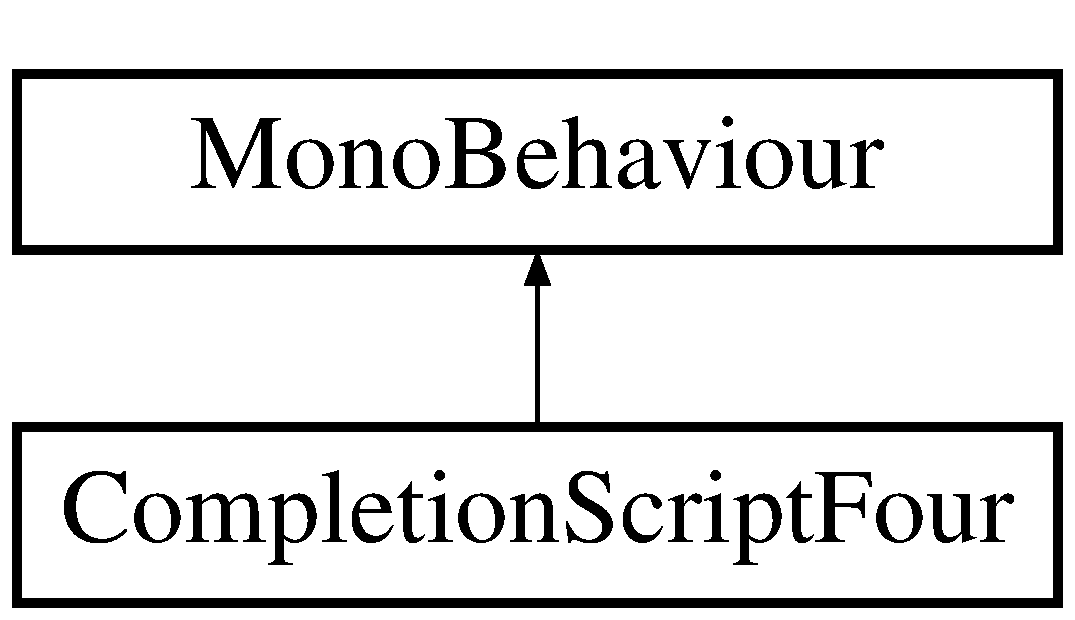
\includegraphics[height=2.000000cm]{class_completion_script_four}
\end{center}
\end{figure}
\subsection*{Public Member Functions}
\begin{DoxyCompactItemize}
\item 
void \hyperlink{class_completion_script_four_ae34b24c5e0545a3e041eddda6ea06767}{reset\+Puzzle} ()
\item 
void \hyperlink{class_completion_script_four_ad52ed9205b311988a64510d048a7fbee}{reset\+Check\+Values} ()
\item 
void \hyperlink{class_completion_script_four_a91395c696c2e4425fbcd205eeccf4754}{reset\+Slots} ()
\item 
void \hyperlink{class_completion_script_four_a427cec802b76d4a42ee5b60427b34f6f}{reset\+Tiles} ()
\item 
void \hyperlink{class_completion_script_four_a49300ed9b78d89b8f68cdf6391925498}{reset\+Active} ()
\end{DoxyCompactItemize}
\subsection*{Public Attributes}
\begin{DoxyCompactItemize}
\item 
\hyperlink{class_array_reaction}{Array\+Reaction} \hyperlink{class_completion_script_four_a747aafbf72eb507c388cb72ad6911b13}{x\+Success}
\item 
\hyperlink{class_array_reaction}{Array\+Reaction} \hyperlink{class_completion_script_four_a0ca2da180578a27db3671b64e3c83aa7}{replacementX}
\item 
\hyperlink{class_array_reaction}{Array\+Reaction} \hyperlink{class_completion_script_four_a7e5f7bcf0c065ea353de75d5d1691ec5}{replacement\+Plus}
\item 
\hyperlink{class_array_reaction}{Array\+Reaction} \hyperlink{class_completion_script_four_ad490db1318afdbb5065effc988b97652}{replacement\+Plus\+Plus}
\item 
bool \hyperlink{class_completion_script_four_a68c845d369b9cbc78be0596acf49040a}{puzzle\+Finished}
\item 
Game\+Object \hyperlink{class_completion_script_four_ac3a10e751902cbc84d5ca93bc321509a}{laser}
\item 
Audio\+Source \hyperlink{class_completion_script_four_ac78527b696de4ff5992bec7fef332014}{solved}
\item 
Game\+Object \mbox{[}$\,$\mbox{]} \hyperlink{class_completion_script_four_afb5331e25190b2ccd25dda02ebc6f2fa}{array\+Tiles}
\item 
Game\+Object \mbox{[}$\,$\mbox{]} \hyperlink{class_completion_script_four_a5f540699a916116acc868e46b2445352}{replacement\+Tiles}
\end{DoxyCompactItemize}


\subsection{Detailed Description}
Checks the respective challenge and makes changes to the game if the user is correct or not Challenge\+: Loop challenge 2 

\subsection{Member Function Documentation}
\mbox{\Hypertarget{class_completion_script_four_a49300ed9b78d89b8f68cdf6391925498}\label{class_completion_script_four_a49300ed9b78d89b8f68cdf6391925498}} 
\index{Completion\+Script\+Four@{Completion\+Script\+Four}!reset\+Active@{reset\+Active}}
\index{reset\+Active@{reset\+Active}!Completion\+Script\+Four@{Completion\+Script\+Four}}
\subsubsection{\texorpdfstring{reset\+Active()}{resetActive()}}
{\footnotesize\ttfamily void Completion\+Script\+Four.\+reset\+Active (\begin{DoxyParamCaption}{ }\end{DoxyParamCaption})}

\mbox{\Hypertarget{class_completion_script_four_ad52ed9205b311988a64510d048a7fbee}\label{class_completion_script_four_ad52ed9205b311988a64510d048a7fbee}} 
\index{Completion\+Script\+Four@{Completion\+Script\+Four}!reset\+Check\+Values@{reset\+Check\+Values}}
\index{reset\+Check\+Values@{reset\+Check\+Values}!Completion\+Script\+Four@{Completion\+Script\+Four}}
\subsubsection{\texorpdfstring{reset\+Check\+Values()}{resetCheckValues()}}
{\footnotesize\ttfamily void Completion\+Script\+Four.\+reset\+Check\+Values (\begin{DoxyParamCaption}{ }\end{DoxyParamCaption})}

\mbox{\Hypertarget{class_completion_script_four_ae34b24c5e0545a3e041eddda6ea06767}\label{class_completion_script_four_ae34b24c5e0545a3e041eddda6ea06767}} 
\index{Completion\+Script\+Four@{Completion\+Script\+Four}!reset\+Puzzle@{reset\+Puzzle}}
\index{reset\+Puzzle@{reset\+Puzzle}!Completion\+Script\+Four@{Completion\+Script\+Four}}
\subsubsection{\texorpdfstring{reset\+Puzzle()}{resetPuzzle()}}
{\footnotesize\ttfamily void Completion\+Script\+Four.\+reset\+Puzzle (\begin{DoxyParamCaption}{ }\end{DoxyParamCaption})}

\mbox{\Hypertarget{class_completion_script_four_a91395c696c2e4425fbcd205eeccf4754}\label{class_completion_script_four_a91395c696c2e4425fbcd205eeccf4754}} 
\index{Completion\+Script\+Four@{Completion\+Script\+Four}!reset\+Slots@{reset\+Slots}}
\index{reset\+Slots@{reset\+Slots}!Completion\+Script\+Four@{Completion\+Script\+Four}}
\subsubsection{\texorpdfstring{reset\+Slots()}{resetSlots()}}
{\footnotesize\ttfamily void Completion\+Script\+Four.\+reset\+Slots (\begin{DoxyParamCaption}{ }\end{DoxyParamCaption})}

\mbox{\Hypertarget{class_completion_script_four_a427cec802b76d4a42ee5b60427b34f6f}\label{class_completion_script_four_a427cec802b76d4a42ee5b60427b34f6f}} 
\index{Completion\+Script\+Four@{Completion\+Script\+Four}!reset\+Tiles@{reset\+Tiles}}
\index{reset\+Tiles@{reset\+Tiles}!Completion\+Script\+Four@{Completion\+Script\+Four}}
\subsubsection{\texorpdfstring{reset\+Tiles()}{resetTiles()}}
{\footnotesize\ttfamily void Completion\+Script\+Four.\+reset\+Tiles (\begin{DoxyParamCaption}{ }\end{DoxyParamCaption})}



\subsection{Member Data Documentation}
\mbox{\Hypertarget{class_completion_script_four_afb5331e25190b2ccd25dda02ebc6f2fa}\label{class_completion_script_four_afb5331e25190b2ccd25dda02ebc6f2fa}} 
\index{Completion\+Script\+Four@{Completion\+Script\+Four}!array\+Tiles@{array\+Tiles}}
\index{array\+Tiles@{array\+Tiles}!Completion\+Script\+Four@{Completion\+Script\+Four}}
\subsubsection{\texorpdfstring{array\+Tiles}{arrayTiles}}
{\footnotesize\ttfamily Game\+Object \mbox{[}$\,$\mbox{]} Completion\+Script\+Four.\+array\+Tiles}

\mbox{\Hypertarget{class_completion_script_four_ac3a10e751902cbc84d5ca93bc321509a}\label{class_completion_script_four_ac3a10e751902cbc84d5ca93bc321509a}} 
\index{Completion\+Script\+Four@{Completion\+Script\+Four}!laser@{laser}}
\index{laser@{laser}!Completion\+Script\+Four@{Completion\+Script\+Four}}
\subsubsection{\texorpdfstring{laser}{laser}}
{\footnotesize\ttfamily Game\+Object Completion\+Script\+Four.\+laser}

\mbox{\Hypertarget{class_completion_script_four_a68c845d369b9cbc78be0596acf49040a}\label{class_completion_script_four_a68c845d369b9cbc78be0596acf49040a}} 
\index{Completion\+Script\+Four@{Completion\+Script\+Four}!puzzle\+Finished@{puzzle\+Finished}}
\index{puzzle\+Finished@{puzzle\+Finished}!Completion\+Script\+Four@{Completion\+Script\+Four}}
\subsubsection{\texorpdfstring{puzzle\+Finished}{puzzleFinished}}
{\footnotesize\ttfamily bool Completion\+Script\+Four.\+puzzle\+Finished}

\mbox{\Hypertarget{class_completion_script_four_a7e5f7bcf0c065ea353de75d5d1691ec5}\label{class_completion_script_four_a7e5f7bcf0c065ea353de75d5d1691ec5}} 
\index{Completion\+Script\+Four@{Completion\+Script\+Four}!replacement\+Plus@{replacement\+Plus}}
\index{replacement\+Plus@{replacement\+Plus}!Completion\+Script\+Four@{Completion\+Script\+Four}}
\subsubsection{\texorpdfstring{replacement\+Plus}{replacementPlus}}
{\footnotesize\ttfamily \hyperlink{class_array_reaction}{Array\+Reaction} Completion\+Script\+Four.\+replacement\+Plus}

\mbox{\Hypertarget{class_completion_script_four_ad490db1318afdbb5065effc988b97652}\label{class_completion_script_four_ad490db1318afdbb5065effc988b97652}} 
\index{Completion\+Script\+Four@{Completion\+Script\+Four}!replacement\+Plus\+Plus@{replacement\+Plus\+Plus}}
\index{replacement\+Plus\+Plus@{replacement\+Plus\+Plus}!Completion\+Script\+Four@{Completion\+Script\+Four}}
\subsubsection{\texorpdfstring{replacement\+Plus\+Plus}{replacementPlusPlus}}
{\footnotesize\ttfamily \hyperlink{class_array_reaction}{Array\+Reaction} Completion\+Script\+Four.\+replacement\+Plus\+Plus}

\mbox{\Hypertarget{class_completion_script_four_a5f540699a916116acc868e46b2445352}\label{class_completion_script_four_a5f540699a916116acc868e46b2445352}} 
\index{Completion\+Script\+Four@{Completion\+Script\+Four}!replacement\+Tiles@{replacement\+Tiles}}
\index{replacement\+Tiles@{replacement\+Tiles}!Completion\+Script\+Four@{Completion\+Script\+Four}}
\subsubsection{\texorpdfstring{replacement\+Tiles}{replacementTiles}}
{\footnotesize\ttfamily Game\+Object \mbox{[}$\,$\mbox{]} Completion\+Script\+Four.\+replacement\+Tiles}

\mbox{\Hypertarget{class_completion_script_four_a0ca2da180578a27db3671b64e3c83aa7}\label{class_completion_script_four_a0ca2da180578a27db3671b64e3c83aa7}} 
\index{Completion\+Script\+Four@{Completion\+Script\+Four}!replacementX@{replacementX}}
\index{replacementX@{replacementX}!Completion\+Script\+Four@{Completion\+Script\+Four}}
\subsubsection{\texorpdfstring{replacementX}{replacementX}}
{\footnotesize\ttfamily \hyperlink{class_array_reaction}{Array\+Reaction} Completion\+Script\+Four.\+replacementX}

\mbox{\Hypertarget{class_completion_script_four_ac78527b696de4ff5992bec7fef332014}\label{class_completion_script_four_ac78527b696de4ff5992bec7fef332014}} 
\index{Completion\+Script\+Four@{Completion\+Script\+Four}!solved@{solved}}
\index{solved@{solved}!Completion\+Script\+Four@{Completion\+Script\+Four}}
\subsubsection{\texorpdfstring{solved}{solved}}
{\footnotesize\ttfamily Audio\+Source Completion\+Script\+Four.\+solved}

\mbox{\Hypertarget{class_completion_script_four_a747aafbf72eb507c388cb72ad6911b13}\label{class_completion_script_four_a747aafbf72eb507c388cb72ad6911b13}} 
\index{Completion\+Script\+Four@{Completion\+Script\+Four}!x\+Success@{x\+Success}}
\index{x\+Success@{x\+Success}!Completion\+Script\+Four@{Completion\+Script\+Four}}
\subsubsection{\texorpdfstring{x\+Success}{xSuccess}}
{\footnotesize\ttfamily \hyperlink{class_array_reaction}{Array\+Reaction} Completion\+Script\+Four.\+x\+Success}



The documentation for this class was generated from the following file\+:\begin{DoxyCompactItemize}
\item 
/\+Users/kwanholloway/git/5001\+Project/\+Game\+Project/\+Assets/\+Scripts/\+Puzzle\+Logic/\+Loop\+Level/\+While\+Puzzle/\hyperlink{_completion_script_four_8cs}{Completion\+Script\+Four.\+cs}\end{DoxyCompactItemize}

\hypertarget{class_completion_script_three}{}\section{Completion\+Script\+Three Class Reference}
\label{class_completion_script_three}\index{Completion\+Script\+Three@{Completion\+Script\+Three}}
Inheritance diagram for Completion\+Script\+Three\+:\begin{figure}[H]
\begin{center}
\leavevmode
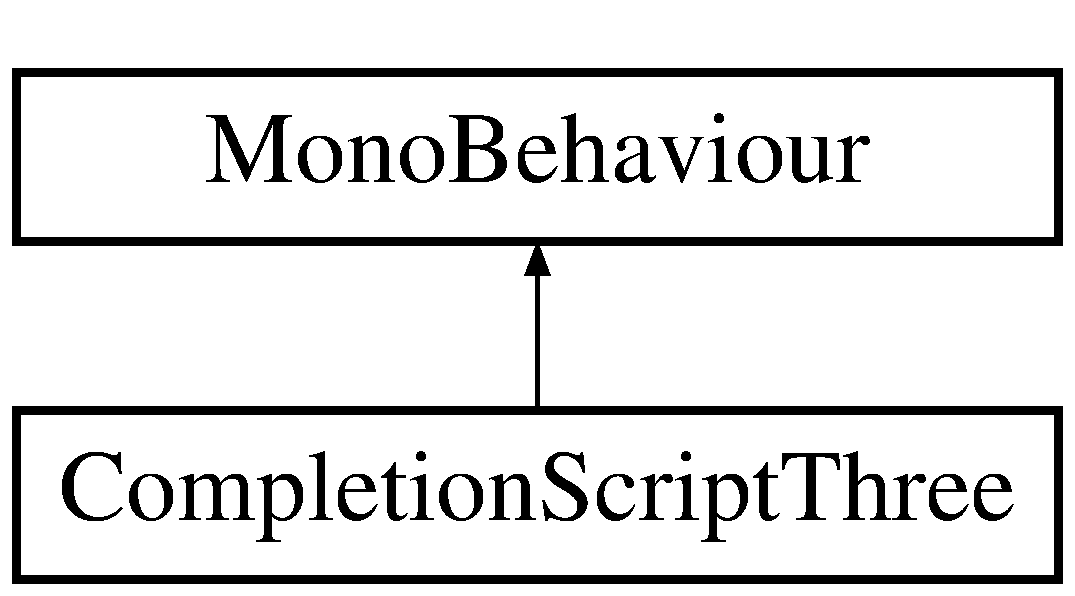
\includegraphics[height=2.000000cm]{class_completion_script_three}
\end{center}
\end{figure}
\subsection*{Public Member Functions}
\begin{DoxyCompactItemize}
\item 
void \hyperlink{class_completion_script_three_a7749647b14b9baf2459c820793551619}{reset\+Puzzle} ()
\item 
void \hyperlink{class_completion_script_three_a45aeee9d673720976534b708fa30d4ba}{reset\+Check\+Values} ()
\item 
void \hyperlink{class_completion_script_three_affbd153c776b7addec8cc060214d1971}{reset\+Slots} ()
\item 
void \hyperlink{class_completion_script_three_aa4c115e628a51c3465153aefa5c80c13}{reset\+Tiles} ()
\item 
void \hyperlink{class_completion_script_three_a1db60c85017b1469f792649b75e9397b}{reset\+Active} ()
\end{DoxyCompactItemize}
\subsection*{Public Attributes}
\begin{DoxyCompactItemize}
\item 
\hyperlink{class_array_reaction}{Array\+Reaction} \hyperlink{class_completion_script_three_a1c12a8282a42059d70e6ef786b9def17}{one\+Success}
\item 
\hyperlink{class_array_reaction}{Array\+Reaction} \hyperlink{class_completion_script_three_adc0fcdc0b8a3acf4f200c86e2af1e3c9}{replacement\+One}
\item 
bool \hyperlink{class_completion_script_three_acff2be49aa067d7a15ae9f8754391be3}{puzzle\+Finished}
\item 
Audio\+Source \hyperlink{class_completion_script_three_ac7eba76f069c14642b9fbbf1dbffd81d}{solved}
\item 
Game\+Object \mbox{[}$\,$\mbox{]} \hyperlink{class_completion_script_three_a8d5751f5f7dd7541d6bcd2fd51206f37}{array\+Tiles}
\item 
Game\+Object \mbox{[}$\,$\mbox{]} \hyperlink{class_completion_script_three_a40c51d90e7210b7da4018ac43dc468f7}{replacement\+Tiles}
\item 
Game\+Object \hyperlink{class_completion_script_three_ab5fc9fb13950a145c8c92e9f5b71001f}{arithmetic\+Portal}
\item 
Game\+Object \hyperlink{class_completion_script_three_a37087f61b2e788fa111e68bc14f50e14}{arith\+Lev\+Tag}
\end{DoxyCompactItemize}


\subsection{Detailed Description}
Checks the respective challenge and makes changes to the game if the user is correct or not Challenge\+: Hub Level Switch challenge 

\subsection{Member Function Documentation}
\mbox{\Hypertarget{class_completion_script_three_a1db60c85017b1469f792649b75e9397b}\label{class_completion_script_three_a1db60c85017b1469f792649b75e9397b}} 
\index{Completion\+Script\+Three@{Completion\+Script\+Three}!reset\+Active@{reset\+Active}}
\index{reset\+Active@{reset\+Active}!Completion\+Script\+Three@{Completion\+Script\+Three}}
\subsubsection{\texorpdfstring{reset\+Active()}{resetActive()}}
{\footnotesize\ttfamily void Completion\+Script\+Three.\+reset\+Active (\begin{DoxyParamCaption}{ }\end{DoxyParamCaption})}

\mbox{\Hypertarget{class_completion_script_three_a45aeee9d673720976534b708fa30d4ba}\label{class_completion_script_three_a45aeee9d673720976534b708fa30d4ba}} 
\index{Completion\+Script\+Three@{Completion\+Script\+Three}!reset\+Check\+Values@{reset\+Check\+Values}}
\index{reset\+Check\+Values@{reset\+Check\+Values}!Completion\+Script\+Three@{Completion\+Script\+Three}}
\subsubsection{\texorpdfstring{reset\+Check\+Values()}{resetCheckValues()}}
{\footnotesize\ttfamily void Completion\+Script\+Three.\+reset\+Check\+Values (\begin{DoxyParamCaption}{ }\end{DoxyParamCaption})}

\mbox{\Hypertarget{class_completion_script_three_a7749647b14b9baf2459c820793551619}\label{class_completion_script_three_a7749647b14b9baf2459c820793551619}} 
\index{Completion\+Script\+Three@{Completion\+Script\+Three}!reset\+Puzzle@{reset\+Puzzle}}
\index{reset\+Puzzle@{reset\+Puzzle}!Completion\+Script\+Three@{Completion\+Script\+Three}}
\subsubsection{\texorpdfstring{reset\+Puzzle()}{resetPuzzle()}}
{\footnotesize\ttfamily void Completion\+Script\+Three.\+reset\+Puzzle (\begin{DoxyParamCaption}{ }\end{DoxyParamCaption})}

\mbox{\Hypertarget{class_completion_script_three_affbd153c776b7addec8cc060214d1971}\label{class_completion_script_three_affbd153c776b7addec8cc060214d1971}} 
\index{Completion\+Script\+Three@{Completion\+Script\+Three}!reset\+Slots@{reset\+Slots}}
\index{reset\+Slots@{reset\+Slots}!Completion\+Script\+Three@{Completion\+Script\+Three}}
\subsubsection{\texorpdfstring{reset\+Slots()}{resetSlots()}}
{\footnotesize\ttfamily void Completion\+Script\+Three.\+reset\+Slots (\begin{DoxyParamCaption}{ }\end{DoxyParamCaption})}

\mbox{\Hypertarget{class_completion_script_three_aa4c115e628a51c3465153aefa5c80c13}\label{class_completion_script_three_aa4c115e628a51c3465153aefa5c80c13}} 
\index{Completion\+Script\+Three@{Completion\+Script\+Three}!reset\+Tiles@{reset\+Tiles}}
\index{reset\+Tiles@{reset\+Tiles}!Completion\+Script\+Three@{Completion\+Script\+Three}}
\subsubsection{\texorpdfstring{reset\+Tiles()}{resetTiles()}}
{\footnotesize\ttfamily void Completion\+Script\+Three.\+reset\+Tiles (\begin{DoxyParamCaption}{ }\end{DoxyParamCaption})}



\subsection{Member Data Documentation}
\mbox{\Hypertarget{class_completion_script_three_a37087f61b2e788fa111e68bc14f50e14}\label{class_completion_script_three_a37087f61b2e788fa111e68bc14f50e14}} 
\index{Completion\+Script\+Three@{Completion\+Script\+Three}!arith\+Lev\+Tag@{arith\+Lev\+Tag}}
\index{arith\+Lev\+Tag@{arith\+Lev\+Tag}!Completion\+Script\+Three@{Completion\+Script\+Three}}
\subsubsection{\texorpdfstring{arith\+Lev\+Tag}{arithLevTag}}
{\footnotesize\ttfamily Game\+Object Completion\+Script\+Three.\+arith\+Lev\+Tag}

\mbox{\Hypertarget{class_completion_script_three_ab5fc9fb13950a145c8c92e9f5b71001f}\label{class_completion_script_three_ab5fc9fb13950a145c8c92e9f5b71001f}} 
\index{Completion\+Script\+Three@{Completion\+Script\+Three}!arithmetic\+Portal@{arithmetic\+Portal}}
\index{arithmetic\+Portal@{arithmetic\+Portal}!Completion\+Script\+Three@{Completion\+Script\+Three}}
\subsubsection{\texorpdfstring{arithmetic\+Portal}{arithmeticPortal}}
{\footnotesize\ttfamily Game\+Object Completion\+Script\+Three.\+arithmetic\+Portal}

\mbox{\Hypertarget{class_completion_script_three_a8d5751f5f7dd7541d6bcd2fd51206f37}\label{class_completion_script_three_a8d5751f5f7dd7541d6bcd2fd51206f37}} 
\index{Completion\+Script\+Three@{Completion\+Script\+Three}!array\+Tiles@{array\+Tiles}}
\index{array\+Tiles@{array\+Tiles}!Completion\+Script\+Three@{Completion\+Script\+Three}}
\subsubsection{\texorpdfstring{array\+Tiles}{arrayTiles}}
{\footnotesize\ttfamily Game\+Object \mbox{[}$\,$\mbox{]} Completion\+Script\+Three.\+array\+Tiles}

\mbox{\Hypertarget{class_completion_script_three_a1c12a8282a42059d70e6ef786b9def17}\label{class_completion_script_three_a1c12a8282a42059d70e6ef786b9def17}} 
\index{Completion\+Script\+Three@{Completion\+Script\+Three}!one\+Success@{one\+Success}}
\index{one\+Success@{one\+Success}!Completion\+Script\+Three@{Completion\+Script\+Three}}
\subsubsection{\texorpdfstring{one\+Success}{oneSuccess}}
{\footnotesize\ttfamily \hyperlink{class_array_reaction}{Array\+Reaction} Completion\+Script\+Three.\+one\+Success}

\mbox{\Hypertarget{class_completion_script_three_acff2be49aa067d7a15ae9f8754391be3}\label{class_completion_script_three_acff2be49aa067d7a15ae9f8754391be3}} 
\index{Completion\+Script\+Three@{Completion\+Script\+Three}!puzzle\+Finished@{puzzle\+Finished}}
\index{puzzle\+Finished@{puzzle\+Finished}!Completion\+Script\+Three@{Completion\+Script\+Three}}
\subsubsection{\texorpdfstring{puzzle\+Finished}{puzzleFinished}}
{\footnotesize\ttfamily bool Completion\+Script\+Three.\+puzzle\+Finished}

\mbox{\Hypertarget{class_completion_script_three_adc0fcdc0b8a3acf4f200c86e2af1e3c9}\label{class_completion_script_three_adc0fcdc0b8a3acf4f200c86e2af1e3c9}} 
\index{Completion\+Script\+Three@{Completion\+Script\+Three}!replacement\+One@{replacement\+One}}
\index{replacement\+One@{replacement\+One}!Completion\+Script\+Three@{Completion\+Script\+Three}}
\subsubsection{\texorpdfstring{replacement\+One}{replacementOne}}
{\footnotesize\ttfamily \hyperlink{class_array_reaction}{Array\+Reaction} Completion\+Script\+Three.\+replacement\+One}

\mbox{\Hypertarget{class_completion_script_three_a40c51d90e7210b7da4018ac43dc468f7}\label{class_completion_script_three_a40c51d90e7210b7da4018ac43dc468f7}} 
\index{Completion\+Script\+Three@{Completion\+Script\+Three}!replacement\+Tiles@{replacement\+Tiles}}
\index{replacement\+Tiles@{replacement\+Tiles}!Completion\+Script\+Three@{Completion\+Script\+Three}}
\subsubsection{\texorpdfstring{replacement\+Tiles}{replacementTiles}}
{\footnotesize\ttfamily Game\+Object \mbox{[}$\,$\mbox{]} Completion\+Script\+Three.\+replacement\+Tiles}

\mbox{\Hypertarget{class_completion_script_three_ac7eba76f069c14642b9fbbf1dbffd81d}\label{class_completion_script_three_ac7eba76f069c14642b9fbbf1dbffd81d}} 
\index{Completion\+Script\+Three@{Completion\+Script\+Three}!solved@{solved}}
\index{solved@{solved}!Completion\+Script\+Three@{Completion\+Script\+Three}}
\subsubsection{\texorpdfstring{solved}{solved}}
{\footnotesize\ttfamily Audio\+Source Completion\+Script\+Three.\+solved}



The documentation for this class was generated from the following file\+:\begin{DoxyCompactItemize}
\item 
/\+Users/kwanholloway/git/5001\+Project/\+Game\+Project/\+Assets/\+Scripts/\+Puzzle\+Logic/\+Switch\+Puzzle/\hyperlink{_completion_script_three_8cs}{Completion\+Script\+Three.\+cs}\end{DoxyCompactItemize}

\hypertarget{class_console}{}\section{Console Class Reference}
\label{class_console}\index{Console@{Console}}
Inheritance diagram for Console\+:\begin{figure}[H]
\begin{center}
\leavevmode
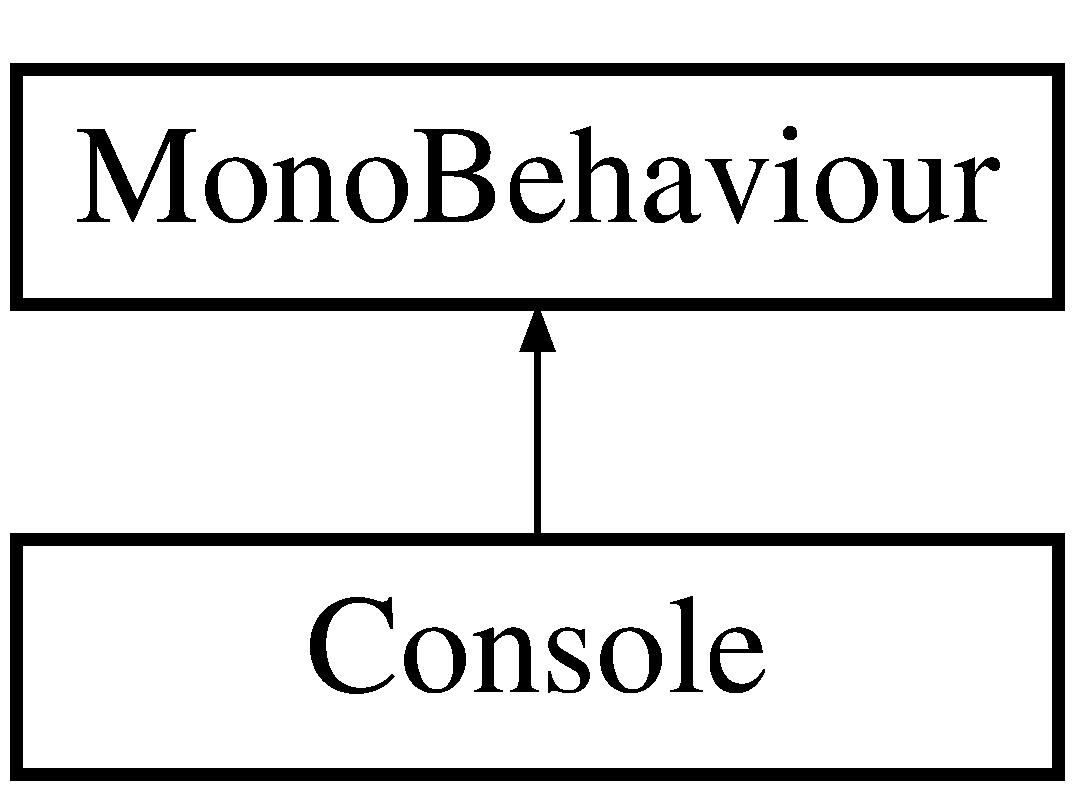
\includegraphics[height=2.000000cm]{class_console}
\end{center}
\end{figure}
\subsection*{Public Attributes}
\begin{DoxyCompactItemize}
\item 
Text \hyperlink{class_console_a6c5f3d4931901e23af8266ca936c7c88}{prompt}
\end{DoxyCompactItemize}


\subsection{Member Data Documentation}
\mbox{\Hypertarget{class_console_a6c5f3d4931901e23af8266ca936c7c88}\label{class_console_a6c5f3d4931901e23af8266ca936c7c88}} 
\index{Console@{Console}!prompt@{prompt}}
\index{prompt@{prompt}!Console@{Console}}
\subsubsection{\texorpdfstring{prompt}{prompt}}
{\footnotesize\ttfamily Text Console.\+prompt}



The documentation for this class was generated from the following file\+:\begin{DoxyCompactItemize}
\item 
/\+Users/kwanholloway/git/5001\+Project/\+Game\+Project/\+Assets/\+Scripts/\+Z-\/\+N\+O\+T U\+S\+E\+D/\hyperlink{_console_8cs}{Console.\+cs}\end{DoxyCompactItemize}

\hypertarget{class_credits_script}{}\section{Credits\+Script Class Reference}
\label{class_credits_script}\index{Credits\+Script@{Credits\+Script}}
Inheritance diagram for Credits\+Script\+:\begin{figure}[H]
\begin{center}
\leavevmode
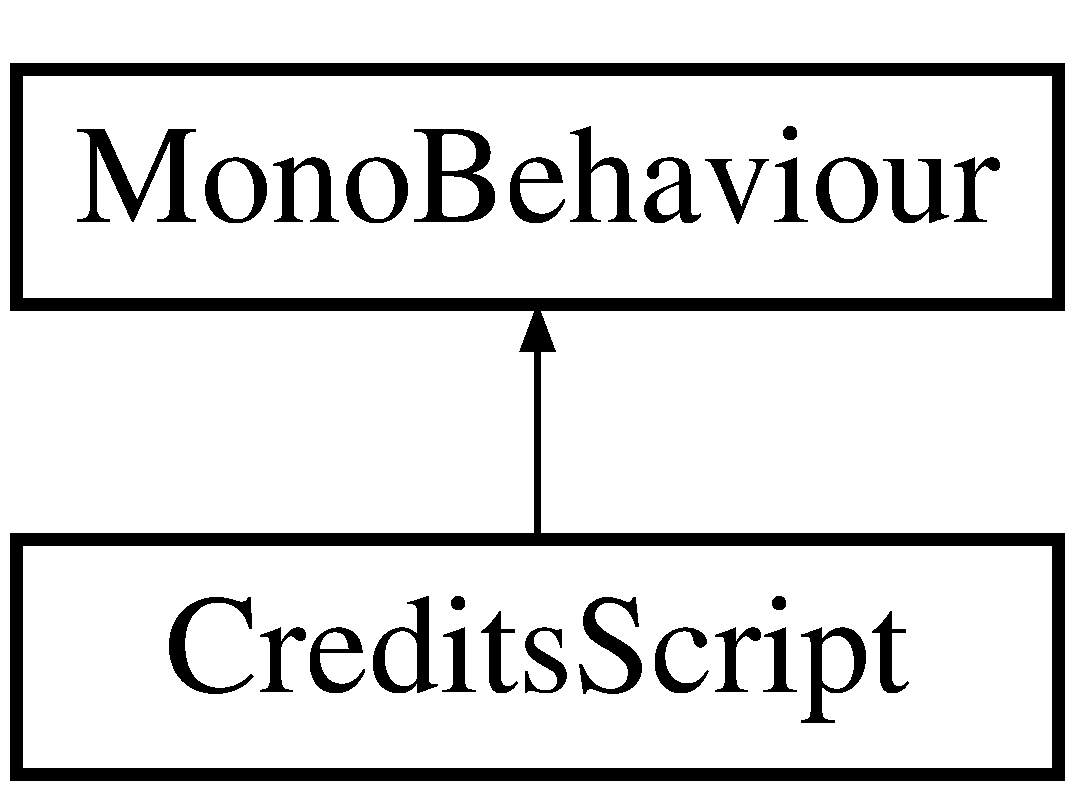
\includegraphics[height=2.000000cm]{class_credits_script}
\end{center}
\end{figure}
\subsection*{Public Member Functions}
\begin{DoxyCompactItemize}
\item 
bool \hyperlink{class_credits_script_ae63ab5451f32c82bda6068facad2a213}{is\+Finished\+Moving} ()
\begin{DoxyCompactList}\small\item\em checks if obj is done moving and returns answer \end{DoxyCompactList}\item 
void \hyperlink{class_credits_script_a6a5a4968b3661e7f2ff3b609c3584957}{set\+Alpha\+To\+Zero} ()
\begin{DoxyCompactList}\small\item\em sets title text, and buttons to be transparent \end{DoxyCompactList}\item 
void \hyperlink{class_credits_script_ad37dc622426ba8d4a4b6a454d4ba81dd}{increase\+Alphas} ()
\begin{DoxyCompactList}\small\item\em sets title text, and buttons to be visible \end{DoxyCompactList}\end{DoxyCompactItemize}
\subsection*{Public Attributes}
\begin{DoxyCompactItemize}
\item 
Game\+Object \hyperlink{class_credits_script_aab6af5235394c7bc904ad65785bc8f31}{obj\+To\+Move}
\item 
Transform \hyperlink{class_credits_script_a1a7ba480a06d7f8bccdb07212e23c6c5}{end\+Point}
\item 
float \hyperlink{class_credits_script_aa10906c5f2d0a86707ec6755d953ea06}{move\+Speed}
\item 
Vector3 \hyperlink{class_credits_script_a592b962a0ac97ed95c8630dad261efe6}{initial\+Position}
\item 
bool \hyperlink{class_credits_script_a830a192ce2ae40b6b57e2e5e84f1bdbf}{finished\+Moving}
\item 
Text \hyperlink{class_credits_script_a82dd5ac0339aa56110dd0e0950a0c4c5}{title\+Text}
\item 
Button \hyperlink{class_credits_script_abe48b2113f4170b2ecd121d3476617e7}{Quit\+Game\+Button}
\end{DoxyCompactItemize}


\subsection{Detailed Description}
Rolls the credits in the Credits scene and manages the buttons that come up afterward 

\subsection{Member Function Documentation}
\mbox{\Hypertarget{class_credits_script_ad37dc622426ba8d4a4b6a454d4ba81dd}\label{class_credits_script_ad37dc622426ba8d4a4b6a454d4ba81dd}} 
\index{Credits\+Script@{Credits\+Script}!increase\+Alphas@{increase\+Alphas}}
\index{increase\+Alphas@{increase\+Alphas}!Credits\+Script@{Credits\+Script}}
\subsubsection{\texorpdfstring{increase\+Alphas()}{increaseAlphas()}}
{\footnotesize\ttfamily void Credits\+Script.\+increase\+Alphas (\begin{DoxyParamCaption}{ }\end{DoxyParamCaption})}



sets title text, and buttons to be visible 

\mbox{\Hypertarget{class_credits_script_ae63ab5451f32c82bda6068facad2a213}\label{class_credits_script_ae63ab5451f32c82bda6068facad2a213}} 
\index{Credits\+Script@{Credits\+Script}!is\+Finished\+Moving@{is\+Finished\+Moving}}
\index{is\+Finished\+Moving@{is\+Finished\+Moving}!Credits\+Script@{Credits\+Script}}
\subsubsection{\texorpdfstring{is\+Finished\+Moving()}{isFinishedMoving()}}
{\footnotesize\ttfamily bool Credits\+Script.\+is\+Finished\+Moving (\begin{DoxyParamCaption}{ }\end{DoxyParamCaption})}



checks if obj is done moving and returns answer 

\mbox{\Hypertarget{class_credits_script_a6a5a4968b3661e7f2ff3b609c3584957}\label{class_credits_script_a6a5a4968b3661e7f2ff3b609c3584957}} 
\index{Credits\+Script@{Credits\+Script}!set\+Alpha\+To\+Zero@{set\+Alpha\+To\+Zero}}
\index{set\+Alpha\+To\+Zero@{set\+Alpha\+To\+Zero}!Credits\+Script@{Credits\+Script}}
\subsubsection{\texorpdfstring{set\+Alpha\+To\+Zero()}{setAlphaToZero()}}
{\footnotesize\ttfamily void Credits\+Script.\+set\+Alpha\+To\+Zero (\begin{DoxyParamCaption}{ }\end{DoxyParamCaption})}



sets title text, and buttons to be transparent 



\subsection{Member Data Documentation}
\mbox{\Hypertarget{class_credits_script_a1a7ba480a06d7f8bccdb07212e23c6c5}\label{class_credits_script_a1a7ba480a06d7f8bccdb07212e23c6c5}} 
\index{Credits\+Script@{Credits\+Script}!end\+Point@{end\+Point}}
\index{end\+Point@{end\+Point}!Credits\+Script@{Credits\+Script}}
\subsubsection{\texorpdfstring{end\+Point}{endPoint}}
{\footnotesize\ttfamily Transform Credits\+Script.\+end\+Point}

\mbox{\Hypertarget{class_credits_script_a830a192ce2ae40b6b57e2e5e84f1bdbf}\label{class_credits_script_a830a192ce2ae40b6b57e2e5e84f1bdbf}} 
\index{Credits\+Script@{Credits\+Script}!finished\+Moving@{finished\+Moving}}
\index{finished\+Moving@{finished\+Moving}!Credits\+Script@{Credits\+Script}}
\subsubsection{\texorpdfstring{finished\+Moving}{finishedMoving}}
{\footnotesize\ttfamily bool Credits\+Script.\+finished\+Moving}

\mbox{\Hypertarget{class_credits_script_a592b962a0ac97ed95c8630dad261efe6}\label{class_credits_script_a592b962a0ac97ed95c8630dad261efe6}} 
\index{Credits\+Script@{Credits\+Script}!initial\+Position@{initial\+Position}}
\index{initial\+Position@{initial\+Position}!Credits\+Script@{Credits\+Script}}
\subsubsection{\texorpdfstring{initial\+Position}{initialPosition}}
{\footnotesize\ttfamily Vector3 Credits\+Script.\+initial\+Position}

\mbox{\Hypertarget{class_credits_script_aa10906c5f2d0a86707ec6755d953ea06}\label{class_credits_script_aa10906c5f2d0a86707ec6755d953ea06}} 
\index{Credits\+Script@{Credits\+Script}!move\+Speed@{move\+Speed}}
\index{move\+Speed@{move\+Speed}!Credits\+Script@{Credits\+Script}}
\subsubsection{\texorpdfstring{move\+Speed}{moveSpeed}}
{\footnotesize\ttfamily float Credits\+Script.\+move\+Speed}

\mbox{\Hypertarget{class_credits_script_aab6af5235394c7bc904ad65785bc8f31}\label{class_credits_script_aab6af5235394c7bc904ad65785bc8f31}} 
\index{Credits\+Script@{Credits\+Script}!obj\+To\+Move@{obj\+To\+Move}}
\index{obj\+To\+Move@{obj\+To\+Move}!Credits\+Script@{Credits\+Script}}
\subsubsection{\texorpdfstring{obj\+To\+Move}{objToMove}}
{\footnotesize\ttfamily Game\+Object Credits\+Script.\+obj\+To\+Move}

\mbox{\Hypertarget{class_credits_script_abe48b2113f4170b2ecd121d3476617e7}\label{class_credits_script_abe48b2113f4170b2ecd121d3476617e7}} 
\index{Credits\+Script@{Credits\+Script}!Quit\+Game\+Button@{Quit\+Game\+Button}}
\index{Quit\+Game\+Button@{Quit\+Game\+Button}!Credits\+Script@{Credits\+Script}}
\subsubsection{\texorpdfstring{Quit\+Game\+Button}{QuitGameButton}}
{\footnotesize\ttfamily Button Credits\+Script.\+Quit\+Game\+Button}

\mbox{\Hypertarget{class_credits_script_a82dd5ac0339aa56110dd0e0950a0c4c5}\label{class_credits_script_a82dd5ac0339aa56110dd0e0950a0c4c5}} 
\index{Credits\+Script@{Credits\+Script}!title\+Text@{title\+Text}}
\index{title\+Text@{title\+Text}!Credits\+Script@{Credits\+Script}}
\subsubsection{\texorpdfstring{title\+Text}{titleText}}
{\footnotesize\ttfamily Text Credits\+Script.\+title\+Text}



The documentation for this class was generated from the following file\+:\begin{DoxyCompactItemize}
\item 
/\+Users/kwanholloway/git/5001\+Project/\+Game\+Project/\+Assets/\+Scripts/\+Game\+Logic/\hyperlink{_credits_script_8cs}{Credits\+Script.\+cs}\end{DoxyCompactItemize}

\hypertarget{class_data_type_completion_check}{}\section{Data\+Type\+Completion\+Check Class Reference}
\label{class_data_type_completion_check}\index{Data\+Type\+Completion\+Check@{Data\+Type\+Completion\+Check}}
Inheritance diagram for Data\+Type\+Completion\+Check\+:\begin{figure}[H]
\begin{center}
\leavevmode
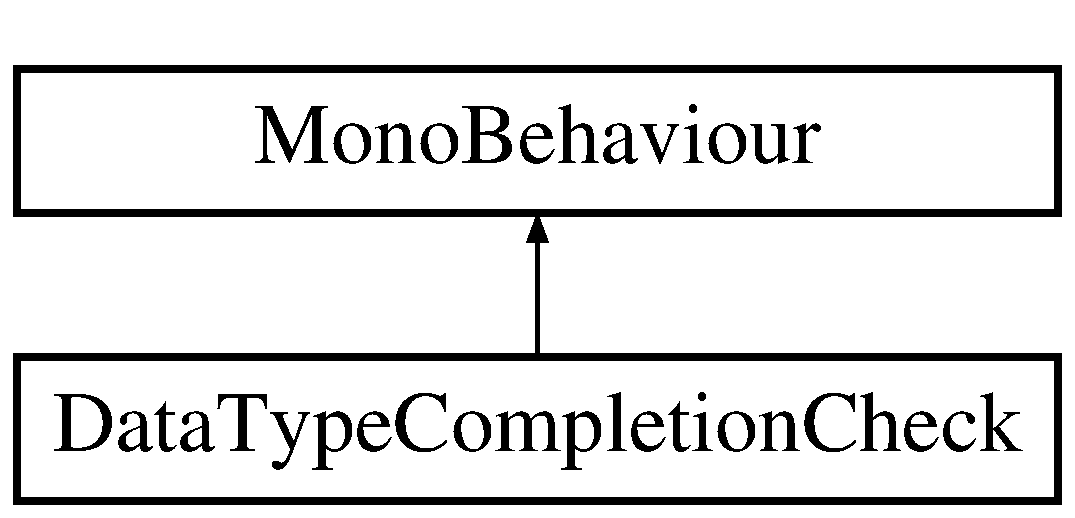
\includegraphics[height=2.000000cm]{class_data_type_completion_check}
\end{center}
\end{figure}
\subsection*{Public Member Functions}
\begin{DoxyCompactItemize}
\item 
void \hyperlink{class_data_type_completion_check_ad3f39d3c444a4c12d9be6d34301d205c}{reset\+Puzzle} ()
\item 
void \hyperlink{class_data_type_completion_check_a67f85080d0dffb91232071fb8309bb03}{reset\+Check\+Values} ()
\item 
void \hyperlink{class_data_type_completion_check_a9bd671a2b59b84e18d2edc73230f6685}{open\+Door} ()
\item 
void \hyperlink{class_data_type_completion_check_afcee752af57f3545637a47ed18dbb323}{close\+Door} ()
\item 
void \hyperlink{class_data_type_completion_check_a9da4ca7a2b766793c7bf5f58b0122353}{reset\+Slots} ()
\item 
void \hyperlink{class_data_type_completion_check_a809e4d0382491e248501c35998e92046}{reset\+Tiles} ()
\item 
void \hyperlink{class_data_type_completion_check_a815b17174f47c02a08e1e3442d895409}{reset\+Active} ()
\item 
bool \hyperlink{class_data_type_completion_check_ac2ed1c70356ebaf4db5ecb26edccda66}{check\+Input\+Success} ()
\item 
bool \hyperlink{class_data_type_completion_check_a508b3241c277e5fa65a9d9510f971946}{check\+Input\+Name} ()
\end{DoxyCompactItemize}
\subsection*{Public Attributes}
\begin{DoxyCompactItemize}
\item 
Game\+Object \mbox{[}$\,$\mbox{]} \hyperlink{class_data_type_completion_check_ace0376e59ce94a6d019a51a160acdfad}{check\+Slots}
\item 
Game\+Object \mbox{[}$\,$\mbox{]} \hyperlink{class_data_type_completion_check_a0ff49d8fba4310d33f2ba4d73c7a4c5c}{array\+Tiles}
\item 
Game\+Object \mbox{[}$\,$\mbox{]} \hyperlink{class_data_type_completion_check_a449d1553d09ac32e51a559a98060a938}{replacement\+Tiles}
\item 
Game\+Object \hyperlink{class_data_type_completion_check_a30fb1fb9074db5c7585e72a1ea4f85d7}{door}
\item 
Audio\+Source \hyperlink{class_data_type_completion_check_ab5a51018023ce893836ccfabf1c73f60}{solved}
\item 
Text \hyperlink{class_data_type_completion_check_ae9a30b339b4e198795dfe7bc2bf57c11}{error\+Message}
\item 
bool \hyperlink{class_data_type_completion_check_a888ca57a6f64ac6e4eefa302a8067986}{puzzle\+Finished}
\end{DoxyCompactItemize}


\subsection{Member Function Documentation}
\mbox{\Hypertarget{class_data_type_completion_check_a508b3241c277e5fa65a9d9510f971946}\label{class_data_type_completion_check_a508b3241c277e5fa65a9d9510f971946}} 
\index{Data\+Type\+Completion\+Check@{Data\+Type\+Completion\+Check}!check\+Input\+Name@{check\+Input\+Name}}
\index{check\+Input\+Name@{check\+Input\+Name}!Data\+Type\+Completion\+Check@{Data\+Type\+Completion\+Check}}
\subsubsection{\texorpdfstring{check\+Input\+Name()}{checkInputName()}}
{\footnotesize\ttfamily bool Data\+Type\+Completion\+Check.\+check\+Input\+Name (\begin{DoxyParamCaption}{ }\end{DoxyParamCaption})}

\mbox{\Hypertarget{class_data_type_completion_check_ac2ed1c70356ebaf4db5ecb26edccda66}\label{class_data_type_completion_check_ac2ed1c70356ebaf4db5ecb26edccda66}} 
\index{Data\+Type\+Completion\+Check@{Data\+Type\+Completion\+Check}!check\+Input\+Success@{check\+Input\+Success}}
\index{check\+Input\+Success@{check\+Input\+Success}!Data\+Type\+Completion\+Check@{Data\+Type\+Completion\+Check}}
\subsubsection{\texorpdfstring{check\+Input\+Success()}{checkInputSuccess()}}
{\footnotesize\ttfamily bool Data\+Type\+Completion\+Check.\+check\+Input\+Success (\begin{DoxyParamCaption}{ }\end{DoxyParamCaption})}

\mbox{\Hypertarget{class_data_type_completion_check_afcee752af57f3545637a47ed18dbb323}\label{class_data_type_completion_check_afcee752af57f3545637a47ed18dbb323}} 
\index{Data\+Type\+Completion\+Check@{Data\+Type\+Completion\+Check}!close\+Door@{close\+Door}}
\index{close\+Door@{close\+Door}!Data\+Type\+Completion\+Check@{Data\+Type\+Completion\+Check}}
\subsubsection{\texorpdfstring{close\+Door()}{closeDoor()}}
{\footnotesize\ttfamily void Data\+Type\+Completion\+Check.\+close\+Door (\begin{DoxyParamCaption}{ }\end{DoxyParamCaption})}

\mbox{\Hypertarget{class_data_type_completion_check_a9bd671a2b59b84e18d2edc73230f6685}\label{class_data_type_completion_check_a9bd671a2b59b84e18d2edc73230f6685}} 
\index{Data\+Type\+Completion\+Check@{Data\+Type\+Completion\+Check}!open\+Door@{open\+Door}}
\index{open\+Door@{open\+Door}!Data\+Type\+Completion\+Check@{Data\+Type\+Completion\+Check}}
\subsubsection{\texorpdfstring{open\+Door()}{openDoor()}}
{\footnotesize\ttfamily void Data\+Type\+Completion\+Check.\+open\+Door (\begin{DoxyParamCaption}{ }\end{DoxyParamCaption})}

\mbox{\Hypertarget{class_data_type_completion_check_a815b17174f47c02a08e1e3442d895409}\label{class_data_type_completion_check_a815b17174f47c02a08e1e3442d895409}} 
\index{Data\+Type\+Completion\+Check@{Data\+Type\+Completion\+Check}!reset\+Active@{reset\+Active}}
\index{reset\+Active@{reset\+Active}!Data\+Type\+Completion\+Check@{Data\+Type\+Completion\+Check}}
\subsubsection{\texorpdfstring{reset\+Active()}{resetActive()}}
{\footnotesize\ttfamily void Data\+Type\+Completion\+Check.\+reset\+Active (\begin{DoxyParamCaption}{ }\end{DoxyParamCaption})}

\mbox{\Hypertarget{class_data_type_completion_check_a67f85080d0dffb91232071fb8309bb03}\label{class_data_type_completion_check_a67f85080d0dffb91232071fb8309bb03}} 
\index{Data\+Type\+Completion\+Check@{Data\+Type\+Completion\+Check}!reset\+Check\+Values@{reset\+Check\+Values}}
\index{reset\+Check\+Values@{reset\+Check\+Values}!Data\+Type\+Completion\+Check@{Data\+Type\+Completion\+Check}}
\subsubsection{\texorpdfstring{reset\+Check\+Values()}{resetCheckValues()}}
{\footnotesize\ttfamily void Data\+Type\+Completion\+Check.\+reset\+Check\+Values (\begin{DoxyParamCaption}{ }\end{DoxyParamCaption})}

\mbox{\Hypertarget{class_data_type_completion_check_ad3f39d3c444a4c12d9be6d34301d205c}\label{class_data_type_completion_check_ad3f39d3c444a4c12d9be6d34301d205c}} 
\index{Data\+Type\+Completion\+Check@{Data\+Type\+Completion\+Check}!reset\+Puzzle@{reset\+Puzzle}}
\index{reset\+Puzzle@{reset\+Puzzle}!Data\+Type\+Completion\+Check@{Data\+Type\+Completion\+Check}}
\subsubsection{\texorpdfstring{reset\+Puzzle()}{resetPuzzle()}}
{\footnotesize\ttfamily void Data\+Type\+Completion\+Check.\+reset\+Puzzle (\begin{DoxyParamCaption}{ }\end{DoxyParamCaption})}

Resets the puzzle Resets the Tiles, slots, check values, camera flag and error message \mbox{\Hypertarget{class_data_type_completion_check_a9da4ca7a2b766793c7bf5f58b0122353}\label{class_data_type_completion_check_a9da4ca7a2b766793c7bf5f58b0122353}} 
\index{Data\+Type\+Completion\+Check@{Data\+Type\+Completion\+Check}!reset\+Slots@{reset\+Slots}}
\index{reset\+Slots@{reset\+Slots}!Data\+Type\+Completion\+Check@{Data\+Type\+Completion\+Check}}
\subsubsection{\texorpdfstring{reset\+Slots()}{resetSlots()}}
{\footnotesize\ttfamily void Data\+Type\+Completion\+Check.\+reset\+Slots (\begin{DoxyParamCaption}{ }\end{DoxyParamCaption})}

\mbox{\Hypertarget{class_data_type_completion_check_a809e4d0382491e248501c35998e92046}\label{class_data_type_completion_check_a809e4d0382491e248501c35998e92046}} 
\index{Data\+Type\+Completion\+Check@{Data\+Type\+Completion\+Check}!reset\+Tiles@{reset\+Tiles}}
\index{reset\+Tiles@{reset\+Tiles}!Data\+Type\+Completion\+Check@{Data\+Type\+Completion\+Check}}
\subsubsection{\texorpdfstring{reset\+Tiles()}{resetTiles()}}
{\footnotesize\ttfamily void Data\+Type\+Completion\+Check.\+reset\+Tiles (\begin{DoxyParamCaption}{ }\end{DoxyParamCaption})}



\subsection{Member Data Documentation}
\mbox{\Hypertarget{class_data_type_completion_check_a0ff49d8fba4310d33f2ba4d73c7a4c5c}\label{class_data_type_completion_check_a0ff49d8fba4310d33f2ba4d73c7a4c5c}} 
\index{Data\+Type\+Completion\+Check@{Data\+Type\+Completion\+Check}!array\+Tiles@{array\+Tiles}}
\index{array\+Tiles@{array\+Tiles}!Data\+Type\+Completion\+Check@{Data\+Type\+Completion\+Check}}
\subsubsection{\texorpdfstring{array\+Tiles}{arrayTiles}}
{\footnotesize\ttfamily Game\+Object \mbox{[}$\,$\mbox{]} Data\+Type\+Completion\+Check.\+array\+Tiles}

\mbox{\Hypertarget{class_data_type_completion_check_ace0376e59ce94a6d019a51a160acdfad}\label{class_data_type_completion_check_ace0376e59ce94a6d019a51a160acdfad}} 
\index{Data\+Type\+Completion\+Check@{Data\+Type\+Completion\+Check}!check\+Slots@{check\+Slots}}
\index{check\+Slots@{check\+Slots}!Data\+Type\+Completion\+Check@{Data\+Type\+Completion\+Check}}
\subsubsection{\texorpdfstring{check\+Slots}{checkSlots}}
{\footnotesize\ttfamily Game\+Object \mbox{[}$\,$\mbox{]} Data\+Type\+Completion\+Check.\+check\+Slots}

\mbox{\Hypertarget{class_data_type_completion_check_a30fb1fb9074db5c7585e72a1ea4f85d7}\label{class_data_type_completion_check_a30fb1fb9074db5c7585e72a1ea4f85d7}} 
\index{Data\+Type\+Completion\+Check@{Data\+Type\+Completion\+Check}!door@{door}}
\index{door@{door}!Data\+Type\+Completion\+Check@{Data\+Type\+Completion\+Check}}
\subsubsection{\texorpdfstring{door}{door}}
{\footnotesize\ttfamily Game\+Object Data\+Type\+Completion\+Check.\+door}

\mbox{\Hypertarget{class_data_type_completion_check_ae9a30b339b4e198795dfe7bc2bf57c11}\label{class_data_type_completion_check_ae9a30b339b4e198795dfe7bc2bf57c11}} 
\index{Data\+Type\+Completion\+Check@{Data\+Type\+Completion\+Check}!error\+Message@{error\+Message}}
\index{error\+Message@{error\+Message}!Data\+Type\+Completion\+Check@{Data\+Type\+Completion\+Check}}
\subsubsection{\texorpdfstring{error\+Message}{errorMessage}}
{\footnotesize\ttfamily Text Data\+Type\+Completion\+Check.\+error\+Message}

\mbox{\Hypertarget{class_data_type_completion_check_a888ca57a6f64ac6e4eefa302a8067986}\label{class_data_type_completion_check_a888ca57a6f64ac6e4eefa302a8067986}} 
\index{Data\+Type\+Completion\+Check@{Data\+Type\+Completion\+Check}!puzzle\+Finished@{puzzle\+Finished}}
\index{puzzle\+Finished@{puzzle\+Finished}!Data\+Type\+Completion\+Check@{Data\+Type\+Completion\+Check}}
\subsubsection{\texorpdfstring{puzzle\+Finished}{puzzleFinished}}
{\footnotesize\ttfamily bool Data\+Type\+Completion\+Check.\+puzzle\+Finished}

\mbox{\Hypertarget{class_data_type_completion_check_a449d1553d09ac32e51a559a98060a938}\label{class_data_type_completion_check_a449d1553d09ac32e51a559a98060a938}} 
\index{Data\+Type\+Completion\+Check@{Data\+Type\+Completion\+Check}!replacement\+Tiles@{replacement\+Tiles}}
\index{replacement\+Tiles@{replacement\+Tiles}!Data\+Type\+Completion\+Check@{Data\+Type\+Completion\+Check}}
\subsubsection{\texorpdfstring{replacement\+Tiles}{replacementTiles}}
{\footnotesize\ttfamily Game\+Object \mbox{[}$\,$\mbox{]} Data\+Type\+Completion\+Check.\+replacement\+Tiles}

\mbox{\Hypertarget{class_data_type_completion_check_ab5a51018023ce893836ccfabf1c73f60}\label{class_data_type_completion_check_ab5a51018023ce893836ccfabf1c73f60}} 
\index{Data\+Type\+Completion\+Check@{Data\+Type\+Completion\+Check}!solved@{solved}}
\index{solved@{solved}!Data\+Type\+Completion\+Check@{Data\+Type\+Completion\+Check}}
\subsubsection{\texorpdfstring{solved}{solved}}
{\footnotesize\ttfamily Audio\+Source Data\+Type\+Completion\+Check.\+solved}



The documentation for this class was generated from the following file\+:\begin{DoxyCompactItemize}
\item 
/\+Users/kwanholloway/git/5001\+Project/\+Game\+Project/\+Assets/\+Scripts/\+Puzzle\+Logic/\+Data\+Type\+Puzzle/\hyperlink{_data_type_completion_check_8cs}{Data\+Type\+Completion\+Check.\+cs}\end{DoxyCompactItemize}

\hypertarget{class_desktop_controller}{}\section{Desktop\+Controller Class Reference}
\label{class_desktop_controller}\index{Desktop\+Controller@{Desktop\+Controller}}
Inheritance diagram for Desktop\+Controller\+:\begin{figure}[H]
\begin{center}
\leavevmode
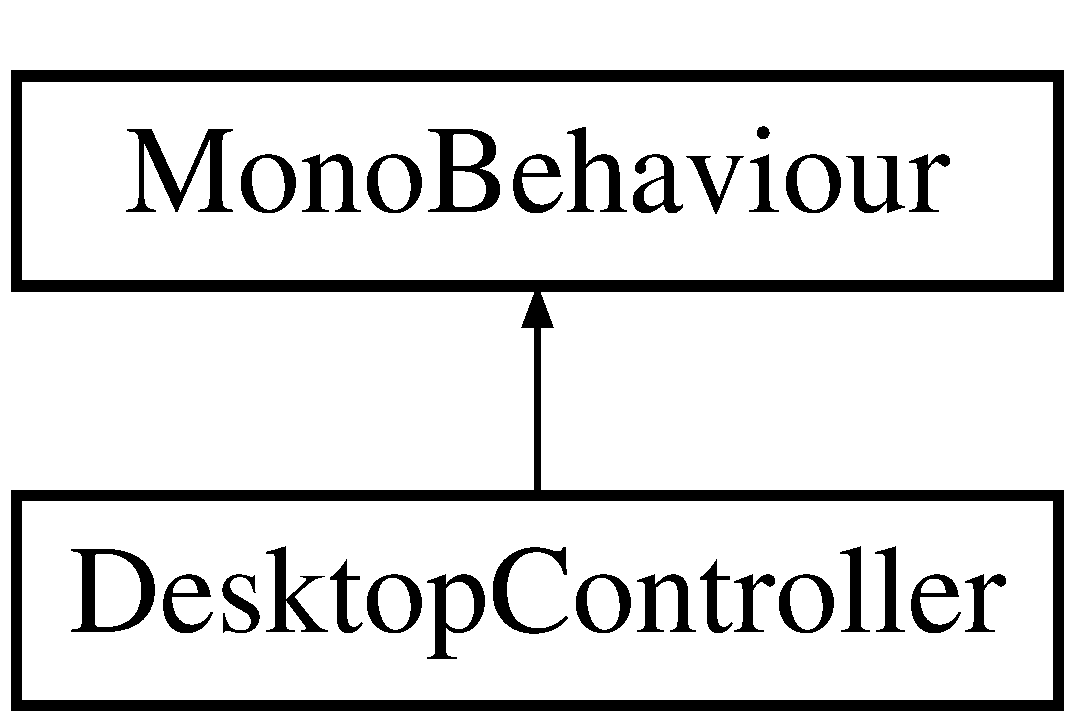
\includegraphics[height=2.000000cm]{class_desktop_controller}
\end{center}
\end{figure}
\subsection*{Public Attributes}
\begin{DoxyCompactItemize}
\item 
Text \hyperlink{class_desktop_controller_a838c18cc5a44e5fb6e1489a390b2c8dd}{prompt}
\end{DoxyCompactItemize}


\subsection{Member Data Documentation}
\mbox{\Hypertarget{class_desktop_controller_a838c18cc5a44e5fb6e1489a390b2c8dd}\label{class_desktop_controller_a838c18cc5a44e5fb6e1489a390b2c8dd}} 
\index{Desktop\+Controller@{Desktop\+Controller}!prompt@{prompt}}
\index{prompt@{prompt}!Desktop\+Controller@{Desktop\+Controller}}
\subsubsection{\texorpdfstring{prompt}{prompt}}
{\footnotesize\ttfamily Text Desktop\+Controller.\+prompt}



The documentation for this class was generated from the following file\+:\begin{DoxyCompactItemize}
\item 
/\+Users/kwanholloway/git/5001\+Project/\+Game\+Project/\+Assets/\+Scripts/\+Puzzle\+Logic/\+Switch\+Puzzle/\hyperlink{_desktop_controller_8cs}{Desktop\+Controller.\+cs}\end{DoxyCompactItemize}

\hypertarget{class_desktop_controller_box_array}{}\section{Desktop\+Controller\+Box\+Array Class Reference}
\label{class_desktop_controller_box_array}\index{Desktop\+Controller\+Box\+Array@{Desktop\+Controller\+Box\+Array}}
Inheritance diagram for Desktop\+Controller\+Box\+Array\+:\begin{figure}[H]
\begin{center}
\leavevmode
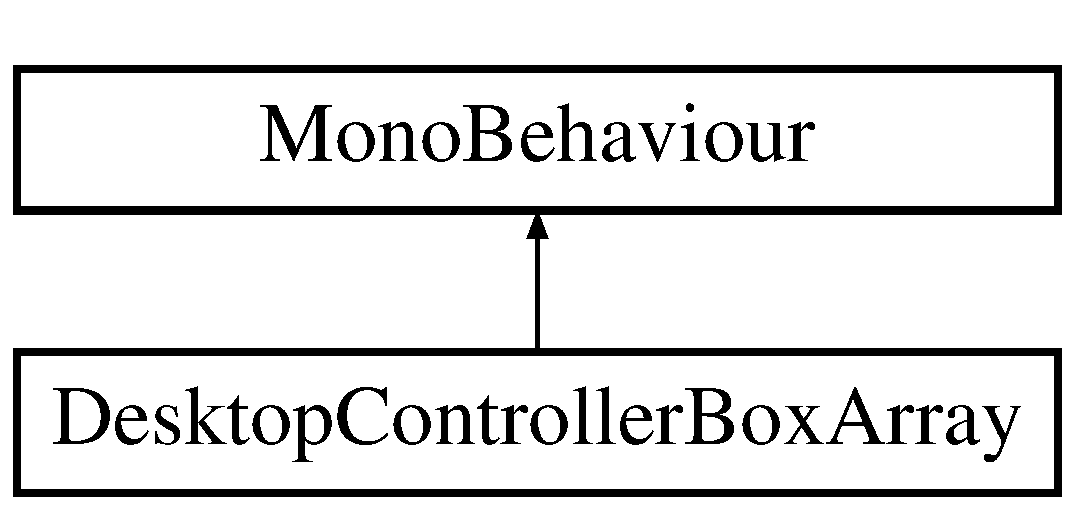
\includegraphics[height=2.000000cm]{class_desktop_controller_box_array}
\end{center}
\end{figure}
\subsection*{Public Attributes}
\begin{DoxyCompactItemize}
\item 
Text \hyperlink{class_desktop_controller_box_array_a947a69388f64d8e59d2836f0836a9538}{prompt}
\item 
Camera \hyperlink{class_desktop_controller_box_array_aceb8f6d6249766e34162daa8fb358b3a}{puzzle\+Camera}
\item 
Camera \hyperlink{class_desktop_controller_box_array_ab959c98f067c77ab701937bd5eb0b7b7}{main\+Cam}
\end{DoxyCompactItemize}


\subsection{Member Data Documentation}
\mbox{\Hypertarget{class_desktop_controller_box_array_ab959c98f067c77ab701937bd5eb0b7b7}\label{class_desktop_controller_box_array_ab959c98f067c77ab701937bd5eb0b7b7}} 
\index{Desktop\+Controller\+Box\+Array@{Desktop\+Controller\+Box\+Array}!main\+Cam@{main\+Cam}}
\index{main\+Cam@{main\+Cam}!Desktop\+Controller\+Box\+Array@{Desktop\+Controller\+Box\+Array}}
\subsubsection{\texorpdfstring{main\+Cam}{mainCam}}
{\footnotesize\ttfamily Camera Desktop\+Controller\+Box\+Array.\+main\+Cam}

\mbox{\Hypertarget{class_desktop_controller_box_array_a947a69388f64d8e59d2836f0836a9538}\label{class_desktop_controller_box_array_a947a69388f64d8e59d2836f0836a9538}} 
\index{Desktop\+Controller\+Box\+Array@{Desktop\+Controller\+Box\+Array}!prompt@{prompt}}
\index{prompt@{prompt}!Desktop\+Controller\+Box\+Array@{Desktop\+Controller\+Box\+Array}}
\subsubsection{\texorpdfstring{prompt}{prompt}}
{\footnotesize\ttfamily Text Desktop\+Controller\+Box\+Array.\+prompt}

\mbox{\Hypertarget{class_desktop_controller_box_array_aceb8f6d6249766e34162daa8fb358b3a}\label{class_desktop_controller_box_array_aceb8f6d6249766e34162daa8fb358b3a}} 
\index{Desktop\+Controller\+Box\+Array@{Desktop\+Controller\+Box\+Array}!puzzle\+Camera@{puzzle\+Camera}}
\index{puzzle\+Camera@{puzzle\+Camera}!Desktop\+Controller\+Box\+Array@{Desktop\+Controller\+Box\+Array}}
\subsubsection{\texorpdfstring{puzzle\+Camera}{puzzleCamera}}
{\footnotesize\ttfamily Camera Desktop\+Controller\+Box\+Array.\+puzzle\+Camera}



The documentation for this class was generated from the following file\+:\begin{DoxyCompactItemize}
\item 
/\+Users/kwanholloway/git/5001\+Project/\+Game\+Project/\+Assets/\+Scripts/\+Array\+Puzzle\+One/\hyperlink{_desktop_controller_box_array_8cs}{Desktop\+Controller\+Box\+Array.\+cs}\end{DoxyCompactItemize}

\hypertarget{class_desktop_interaction}{}\section{Desktop\+Interaction Class Reference}
\label{class_desktop_interaction}\index{Desktop\+Interaction@{Desktop\+Interaction}}
Inheritance diagram for Desktop\+Interaction\+:\begin{figure}[H]
\begin{center}
\leavevmode
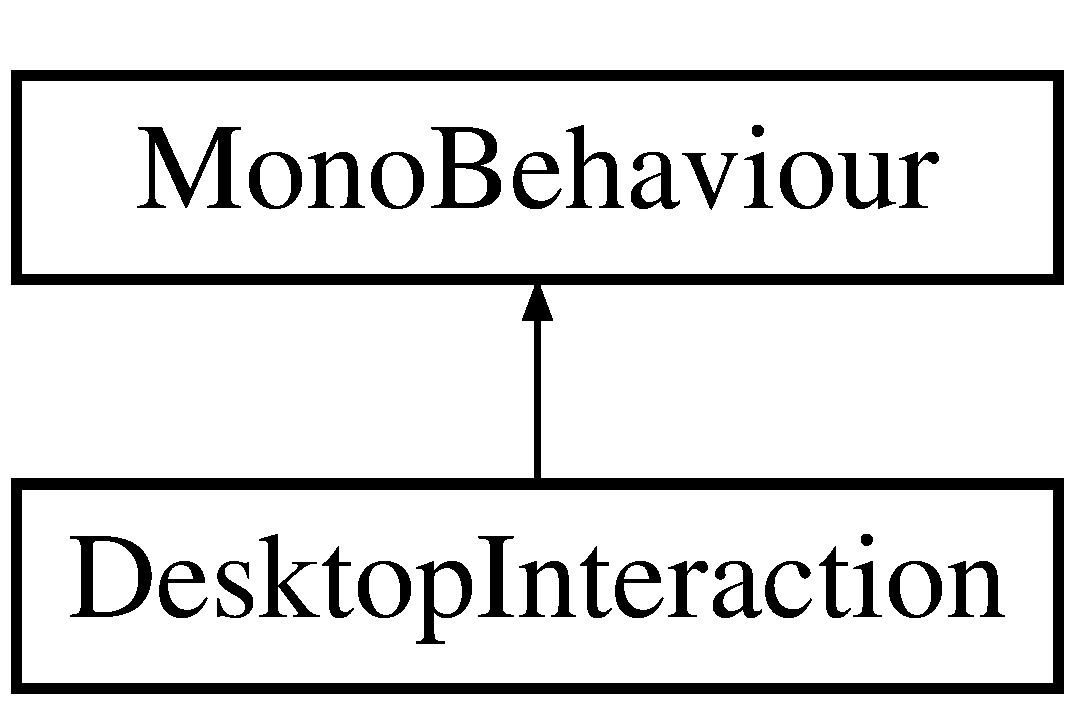
\includegraphics[height=2.000000cm]{class_desktop_interaction}
\end{center}
\end{figure}
\subsection*{Public Attributes}
\begin{DoxyCompactItemize}
\item 
Text \hyperlink{class_desktop_interaction_aaaa52b3abff9c12d9608954274d59741}{prompt}
\item 
Camera \hyperlink{class_desktop_interaction_acf4984e2694edc76dd5fa0ca18559d76}{puzzle\+Camera}
\end{DoxyCompactItemize}


\subsection{Detailed Description}
Class used to allows all desktops to show their respective challenges Also displays a interact prompt when near them 

\subsection{Member Data Documentation}
\mbox{\Hypertarget{class_desktop_interaction_aaaa52b3abff9c12d9608954274d59741}\label{class_desktop_interaction_aaaa52b3abff9c12d9608954274d59741}} 
\index{Desktop\+Interaction@{Desktop\+Interaction}!prompt@{prompt}}
\index{prompt@{prompt}!Desktop\+Interaction@{Desktop\+Interaction}}
\subsubsection{\texorpdfstring{prompt}{prompt}}
{\footnotesize\ttfamily Text Desktop\+Interaction.\+prompt}

\mbox{\Hypertarget{class_desktop_interaction_acf4984e2694edc76dd5fa0ca18559d76}\label{class_desktop_interaction_acf4984e2694edc76dd5fa0ca18559d76}} 
\index{Desktop\+Interaction@{Desktop\+Interaction}!puzzle\+Camera@{puzzle\+Camera}}
\index{puzzle\+Camera@{puzzle\+Camera}!Desktop\+Interaction@{Desktop\+Interaction}}
\subsubsection{\texorpdfstring{puzzle\+Camera}{puzzleCamera}}
{\footnotesize\ttfamily Camera Desktop\+Interaction.\+puzzle\+Camera}



The documentation for this class was generated from the following file\+:\begin{DoxyCompactItemize}
\item 
/\+Users/kwanholloway/git/5001\+Project/\+Game\+Project/\+Assets/\+Scripts/\+Game\+Logic/\hyperlink{_desktop_interaction_8cs}{Desktop\+Interaction.\+cs}\end{DoxyCompactItemize}

\hypertarget{class_elevator_controller}{}\section{Elevator\+Controller Class Reference}
\label{class_elevator_controller}\index{Elevator\+Controller@{Elevator\+Controller}}
Inheritance diagram for Elevator\+Controller\+:\begin{figure}[H]
\begin{center}
\leavevmode
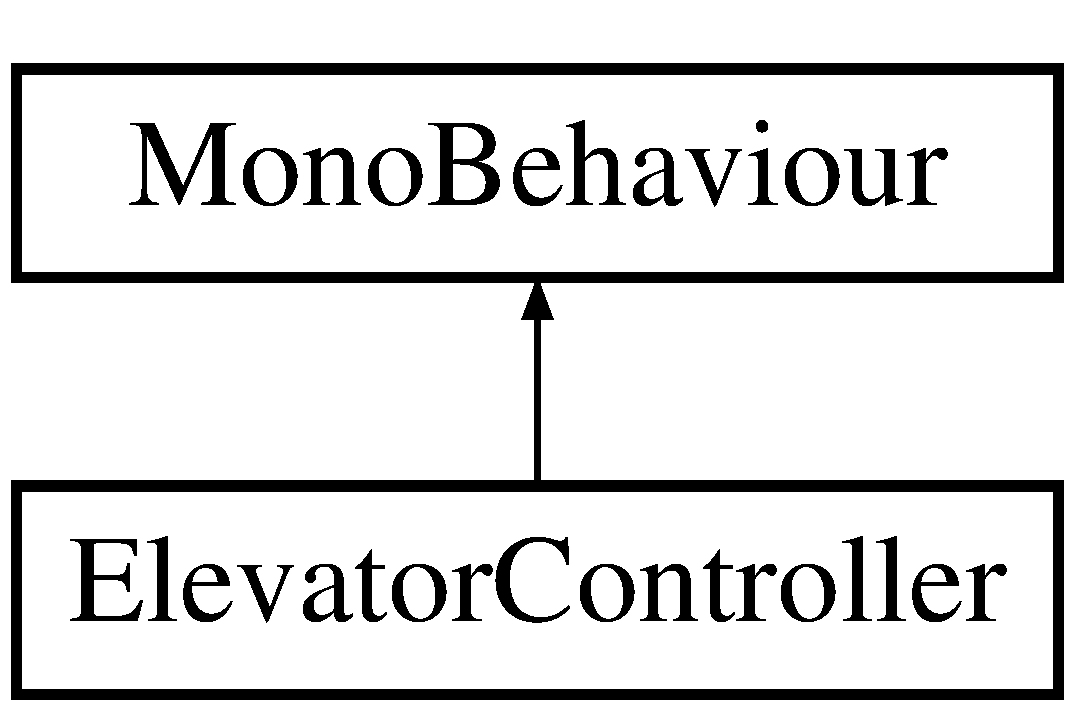
\includegraphics[height=2.000000cm]{class_elevator_controller}
\end{center}
\end{figure}
\subsection*{Public Attributes}
\begin{DoxyCompactItemize}
\item 
Transform \hyperlink{class_elevator_controller_a6e7efcdcf445a847b7d3409662cce3f1}{start\+Marker}
\item 
Game\+Object \hyperlink{class_elevator_controller_a0a95ba162783ed8f0ef35e5ba9494fc6}{player}
\item 
float \hyperlink{class_elevator_controller_a9a5b319532f7be14eeee9d45cf21f695}{up\+Speed} = .\+5f
\item 
float \hyperlink{class_elevator_controller_a127024ceeb58e782d98e76c29c785bd7}{down\+Speed} = .\+15f
\item 
Audio\+Source \hyperlink{class_elevator_controller_ab5b5244289dd36e6a4e480f9cf4269c0}{elevator}
\item 
bool \hyperlink{class_elevator_controller_a092a7e98dc1ca5ccaee15195746f0b59}{in\+Area} = false
\item 
bool \hyperlink{class_elevator_controller_aff0b538f1ab6bf0759c7fde9fcc1fb38}{up} = false
\item 
bool \hyperlink{class_elevator_controller_a10f89ddcc125d36c4bc7958ed94ad2ef}{down} = false
\item 
bool \hyperlink{class_elevator_controller_ab957a12ff569718351939c9b947071a6}{sound\+Flag}
\item 
\hyperlink{class_bool_ops_completion}{Bool\+Ops\+Completion} \hyperlink{class_elevator_controller_a3c7120c81b5845ad6a56167e5a372b38}{elevator\+Flag}
\item 
Camera \hyperlink{class_elevator_controller_af00b8987026003654213434dfd06817e}{logical\+And\+Camera}
\end{DoxyCompactItemize}


\subsection{Member Data Documentation}
\mbox{\Hypertarget{class_elevator_controller_a10f89ddcc125d36c4bc7958ed94ad2ef}\label{class_elevator_controller_a10f89ddcc125d36c4bc7958ed94ad2ef}} 
\index{Elevator\+Controller@{Elevator\+Controller}!down@{down}}
\index{down@{down}!Elevator\+Controller@{Elevator\+Controller}}
\subsubsection{\texorpdfstring{down}{down}}
{\footnotesize\ttfamily bool Elevator\+Controller.\+down = false}

\mbox{\Hypertarget{class_elevator_controller_a127024ceeb58e782d98e76c29c785bd7}\label{class_elevator_controller_a127024ceeb58e782d98e76c29c785bd7}} 
\index{Elevator\+Controller@{Elevator\+Controller}!down\+Speed@{down\+Speed}}
\index{down\+Speed@{down\+Speed}!Elevator\+Controller@{Elevator\+Controller}}
\subsubsection{\texorpdfstring{down\+Speed}{downSpeed}}
{\footnotesize\ttfamily float Elevator\+Controller.\+down\+Speed = .\+15f}

\mbox{\Hypertarget{class_elevator_controller_ab5b5244289dd36e6a4e480f9cf4269c0}\label{class_elevator_controller_ab5b5244289dd36e6a4e480f9cf4269c0}} 
\index{Elevator\+Controller@{Elevator\+Controller}!elevator@{elevator}}
\index{elevator@{elevator}!Elevator\+Controller@{Elevator\+Controller}}
\subsubsection{\texorpdfstring{elevator}{elevator}}
{\footnotesize\ttfamily Audio\+Source Elevator\+Controller.\+elevator}

\mbox{\Hypertarget{class_elevator_controller_a3c7120c81b5845ad6a56167e5a372b38}\label{class_elevator_controller_a3c7120c81b5845ad6a56167e5a372b38}} 
\index{Elevator\+Controller@{Elevator\+Controller}!elevator\+Flag@{elevator\+Flag}}
\index{elevator\+Flag@{elevator\+Flag}!Elevator\+Controller@{Elevator\+Controller}}
\subsubsection{\texorpdfstring{elevator\+Flag}{elevatorFlag}}
{\footnotesize\ttfamily \hyperlink{class_bool_ops_completion}{Bool\+Ops\+Completion} Elevator\+Controller.\+elevator\+Flag}

\mbox{\Hypertarget{class_elevator_controller_a092a7e98dc1ca5ccaee15195746f0b59}\label{class_elevator_controller_a092a7e98dc1ca5ccaee15195746f0b59}} 
\index{Elevator\+Controller@{Elevator\+Controller}!in\+Area@{in\+Area}}
\index{in\+Area@{in\+Area}!Elevator\+Controller@{Elevator\+Controller}}
\subsubsection{\texorpdfstring{in\+Area}{inArea}}
{\footnotesize\ttfamily bool Elevator\+Controller.\+in\+Area = false}

\mbox{\Hypertarget{class_elevator_controller_af00b8987026003654213434dfd06817e}\label{class_elevator_controller_af00b8987026003654213434dfd06817e}} 
\index{Elevator\+Controller@{Elevator\+Controller}!logical\+And\+Camera@{logical\+And\+Camera}}
\index{logical\+And\+Camera@{logical\+And\+Camera}!Elevator\+Controller@{Elevator\+Controller}}
\subsubsection{\texorpdfstring{logical\+And\+Camera}{logicalAndCamera}}
{\footnotesize\ttfamily Camera Elevator\+Controller.\+logical\+And\+Camera}

\mbox{\Hypertarget{class_elevator_controller_a0a95ba162783ed8f0ef35e5ba9494fc6}\label{class_elevator_controller_a0a95ba162783ed8f0ef35e5ba9494fc6}} 
\index{Elevator\+Controller@{Elevator\+Controller}!player@{player}}
\index{player@{player}!Elevator\+Controller@{Elevator\+Controller}}
\subsubsection{\texorpdfstring{player}{player}}
{\footnotesize\ttfamily Game\+Object Elevator\+Controller.\+player}

\mbox{\Hypertarget{class_elevator_controller_ab957a12ff569718351939c9b947071a6}\label{class_elevator_controller_ab957a12ff569718351939c9b947071a6}} 
\index{Elevator\+Controller@{Elevator\+Controller}!sound\+Flag@{sound\+Flag}}
\index{sound\+Flag@{sound\+Flag}!Elevator\+Controller@{Elevator\+Controller}}
\subsubsection{\texorpdfstring{sound\+Flag}{soundFlag}}
{\footnotesize\ttfamily bool Elevator\+Controller.\+sound\+Flag}

\mbox{\Hypertarget{class_elevator_controller_a6e7efcdcf445a847b7d3409662cce3f1}\label{class_elevator_controller_a6e7efcdcf445a847b7d3409662cce3f1}} 
\index{Elevator\+Controller@{Elevator\+Controller}!start\+Marker@{start\+Marker}}
\index{start\+Marker@{start\+Marker}!Elevator\+Controller@{Elevator\+Controller}}
\subsubsection{\texorpdfstring{start\+Marker}{startMarker}}
{\footnotesize\ttfamily Transform Elevator\+Controller.\+start\+Marker}

\mbox{\Hypertarget{class_elevator_controller_aff0b538f1ab6bf0759c7fde9fcc1fb38}\label{class_elevator_controller_aff0b538f1ab6bf0759c7fde9fcc1fb38}} 
\index{Elevator\+Controller@{Elevator\+Controller}!up@{up}}
\index{up@{up}!Elevator\+Controller@{Elevator\+Controller}}
\subsubsection{\texorpdfstring{up}{up}}
{\footnotesize\ttfamily bool Elevator\+Controller.\+up = false}

\mbox{\Hypertarget{class_elevator_controller_a9a5b319532f7be14eeee9d45cf21f695}\label{class_elevator_controller_a9a5b319532f7be14eeee9d45cf21f695}} 
\index{Elevator\+Controller@{Elevator\+Controller}!up\+Speed@{up\+Speed}}
\index{up\+Speed@{up\+Speed}!Elevator\+Controller@{Elevator\+Controller}}
\subsubsection{\texorpdfstring{up\+Speed}{upSpeed}}
{\footnotesize\ttfamily float Elevator\+Controller.\+up\+Speed = .\+5f}



The documentation for this class was generated from the following file\+:\begin{DoxyCompactItemize}
\item 
/\+Users/kwanholloway/git/5001\+Project/\+Game\+Project/\+Assets/\+Scripts/\+Game\+Logic/\hyperlink{_elevator_controller_8cs}{Elevator\+Controller.\+cs}\end{DoxyCompactItemize}

\hypertarget{class_e_s_c_p_o_d___control}{}\section{E\+S\+C\+P\+O\+D\+\_\+\+Control Class Reference}
\label{class_e_s_c_p_o_d___control}\index{E\+S\+C\+P\+O\+D\+\_\+\+Control@{E\+S\+C\+P\+O\+D\+\_\+\+Control}}
Inheritance diagram for E\+S\+C\+P\+O\+D\+\_\+\+Control\+:\begin{figure}[H]
\begin{center}
\leavevmode
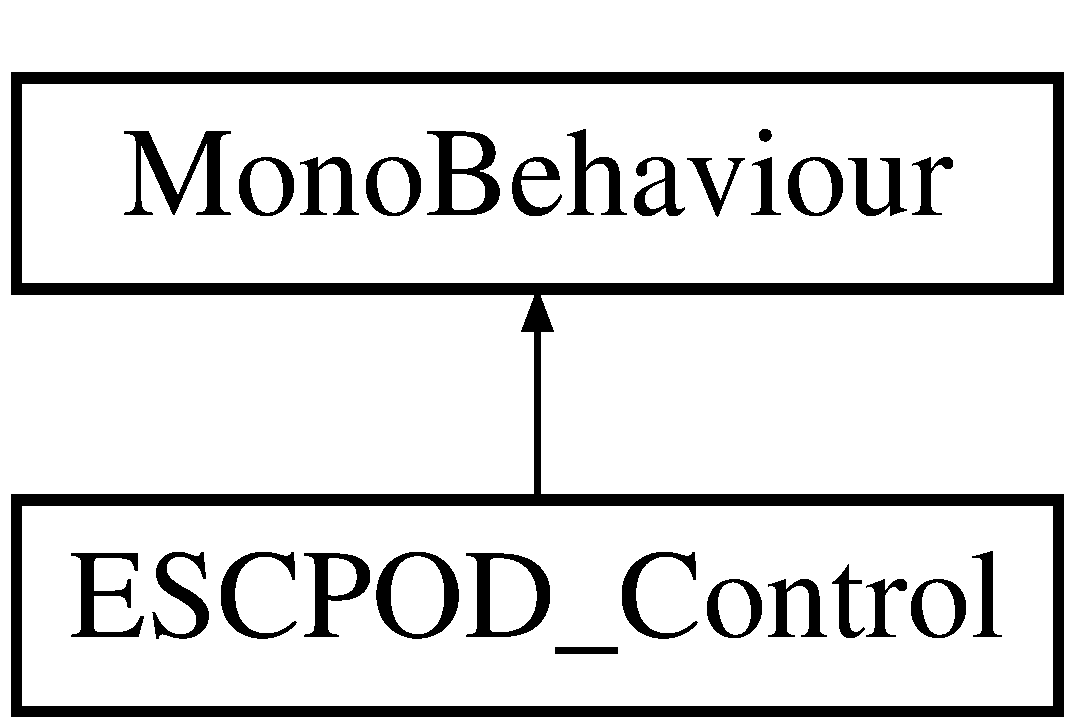
\includegraphics[height=2.000000cm]{class_e_s_c_p_o_d___control}
\end{center}
\end{figure}
\subsection*{Public Attributes}
\begin{DoxyCompactItemize}
\item 
Game\+Object \hyperlink{class_e_s_c_p_o_d___control_a94e64c0ea528fb7c2691ebd0b018197a}{wall1}
\end{DoxyCompactItemize}


\subsection{Detailed Description}
Controls the walls on the escape pod so thet the player doesn\textquotesingle{}t fall tot heir doom 

\subsection{Member Data Documentation}
\mbox{\Hypertarget{class_e_s_c_p_o_d___control_a94e64c0ea528fb7c2691ebd0b018197a}\label{class_e_s_c_p_o_d___control_a94e64c0ea528fb7c2691ebd0b018197a}} 
\index{E\+S\+C\+P\+O\+D\+\_\+\+Control@{E\+S\+C\+P\+O\+D\+\_\+\+Control}!wall1@{wall1}}
\index{wall1@{wall1}!E\+S\+C\+P\+O\+D\+\_\+\+Control@{E\+S\+C\+P\+O\+D\+\_\+\+Control}}
\subsubsection{\texorpdfstring{wall1}{wall1}}
{\footnotesize\ttfamily Game\+Object E\+S\+C\+P\+O\+D\+\_\+\+Control.\+wall1}



The documentation for this class was generated from the following file\+:\begin{DoxyCompactItemize}
\item 
/\+Users/kwanholloway/git/5001\+Project/\+Game\+Project/\+Assets/\+Scripts/\+Game\+Logic/\hyperlink{_e_s_c_p_o_d___control_8cs}{E\+S\+C\+P\+O\+D\+\_\+\+Control.\+cs}\end{DoxyCompactItemize}

\hypertarget{class_e_s_c_p_o_d___control2}{}\section{E\+S\+C\+P\+O\+D\+\_\+\+Control2 Class Reference}
\label{class_e_s_c_p_o_d___control2}\index{E\+S\+C\+P\+O\+D\+\_\+\+Control2@{E\+S\+C\+P\+O\+D\+\_\+\+Control2}}
Inheritance diagram for E\+S\+C\+P\+O\+D\+\_\+\+Control2\+:\begin{figure}[H]
\begin{center}
\leavevmode
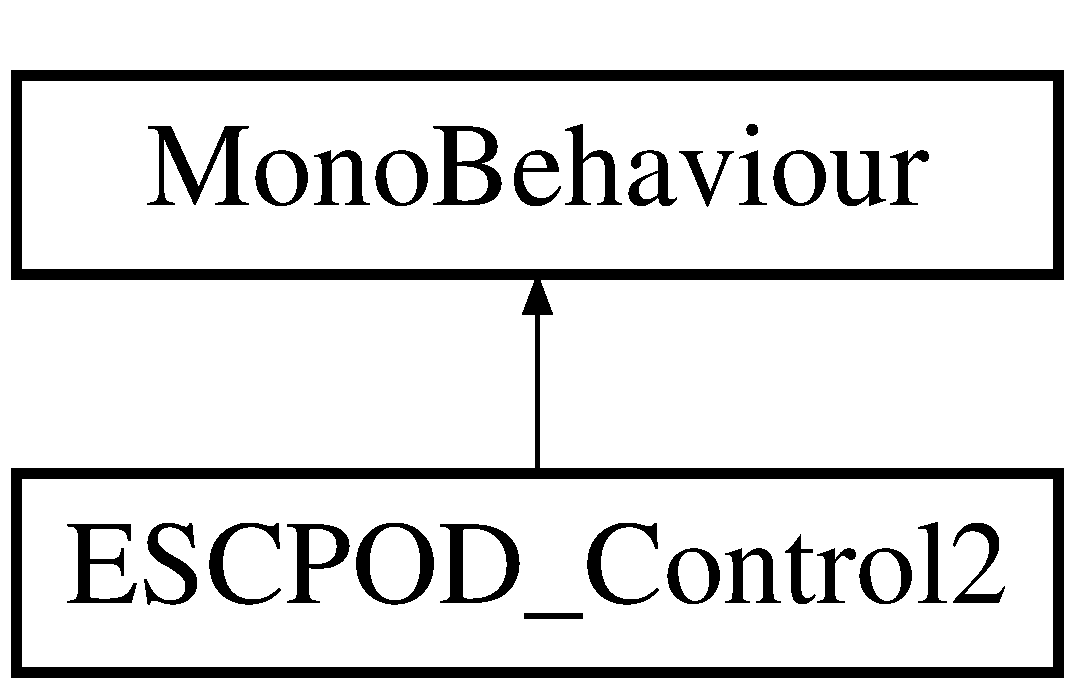
\includegraphics[height=2.000000cm]{class_e_s_c_p_o_d___control2}
\end{center}
\end{figure}
\subsection*{Public Attributes}
\begin{DoxyCompactItemize}
\item 
Game\+Object \hyperlink{class_e_s_c_p_o_d___control2_a5dc074a98094f8c896ba51e19f21c65d}{wall1}
\end{DoxyCompactItemize}


\subsection{Member Data Documentation}
\mbox{\Hypertarget{class_e_s_c_p_o_d___control2_a5dc074a98094f8c896ba51e19f21c65d}\label{class_e_s_c_p_o_d___control2_a5dc074a98094f8c896ba51e19f21c65d}} 
\index{E\+S\+C\+P\+O\+D\+\_\+\+Control2@{E\+S\+C\+P\+O\+D\+\_\+\+Control2}!wall1@{wall1}}
\index{wall1@{wall1}!E\+S\+C\+P\+O\+D\+\_\+\+Control2@{E\+S\+C\+P\+O\+D\+\_\+\+Control2}}
\subsubsection{\texorpdfstring{wall1}{wall1}}
{\footnotesize\ttfamily Game\+Object E\+S\+C\+P\+O\+D\+\_\+\+Control2.\+wall1}



The documentation for this class was generated from the following file\+:\begin{DoxyCompactItemize}
\item 
/\+Users/kwanholloway/git/5001\+Project/\+Game\+Project/\+Assets/\+Scripts/\+Game\+Logic/\hyperlink{_e_s_c_p_o_d___control2_8cs}{E\+S\+C\+P\+O\+D\+\_\+\+Control2.\+cs}\end{DoxyCompactItemize}

\hypertarget{class_exit_door_logic_conditionals}{}\section{Exit\+Door\+Logic\+Conditionals Class Reference}
\label{class_exit_door_logic_conditionals}\index{Exit\+Door\+Logic\+Conditionals@{Exit\+Door\+Logic\+Conditionals}}
Inheritance diagram for Exit\+Door\+Logic\+Conditionals\+:\begin{figure}[H]
\begin{center}
\leavevmode
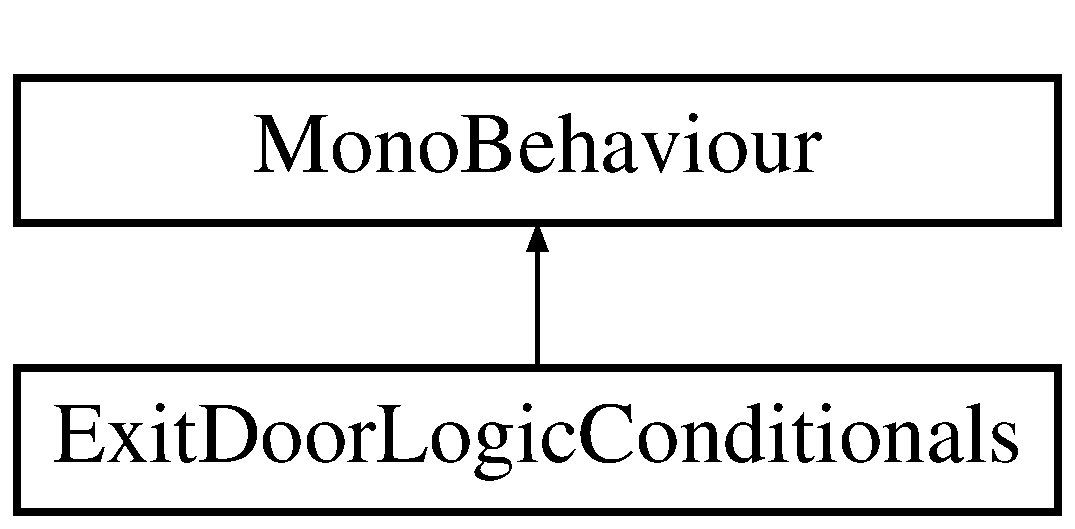
\includegraphics[height=2.000000cm]{class_exit_door_logic_conditionals}
\end{center}
\end{figure}
\subsection*{Public Attributes}
\begin{DoxyCompactItemize}
\item 
bool \hyperlink{class_exit_door_logic_conditionals_acbcfa846f3d5327c2c33804410db1917}{check\+Flag}
\item 
Game\+Object \hyperlink{class_exit_door_logic_conditionals_a49f38a550fb785a6515f412aaccd4231}{exit\+Door}
\end{DoxyCompactItemize}


\subsection{Member Data Documentation}
\mbox{\Hypertarget{class_exit_door_logic_conditionals_acbcfa846f3d5327c2c33804410db1917}\label{class_exit_door_logic_conditionals_acbcfa846f3d5327c2c33804410db1917}} 
\index{Exit\+Door\+Logic\+Conditionals@{Exit\+Door\+Logic\+Conditionals}!check\+Flag@{check\+Flag}}
\index{check\+Flag@{check\+Flag}!Exit\+Door\+Logic\+Conditionals@{Exit\+Door\+Logic\+Conditionals}}
\subsubsection{\texorpdfstring{check\+Flag}{checkFlag}}
{\footnotesize\ttfamily bool Exit\+Door\+Logic\+Conditionals.\+check\+Flag}

\mbox{\Hypertarget{class_exit_door_logic_conditionals_a49f38a550fb785a6515f412aaccd4231}\label{class_exit_door_logic_conditionals_a49f38a550fb785a6515f412aaccd4231}} 
\index{Exit\+Door\+Logic\+Conditionals@{Exit\+Door\+Logic\+Conditionals}!exit\+Door@{exit\+Door}}
\index{exit\+Door@{exit\+Door}!Exit\+Door\+Logic\+Conditionals@{Exit\+Door\+Logic\+Conditionals}}
\subsubsection{\texorpdfstring{exit\+Door}{exitDoor}}
{\footnotesize\ttfamily Game\+Object Exit\+Door\+Logic\+Conditionals.\+exit\+Door}



The documentation for this class was generated from the following file\+:\begin{DoxyCompactItemize}
\item 
/\+Users/kwanholloway/git/5001\+Project/\+Game\+Project/\+Assets/\+Scripts/\+Puzzle\+Logic/\+Conditional Level/\hyperlink{_exit_door_logic_conditionals_8cs}{Exit\+Door\+Logic\+Conditionals.\+cs}\end{DoxyCompactItemize}

\hypertarget{classexplode_logic}{}\section{explode\+Logic Class Reference}
\label{classexplode_logic}\index{explode\+Logic@{explode\+Logic}}
Inheritance diagram for explode\+Logic\+:\begin{figure}[H]
\begin{center}
\leavevmode
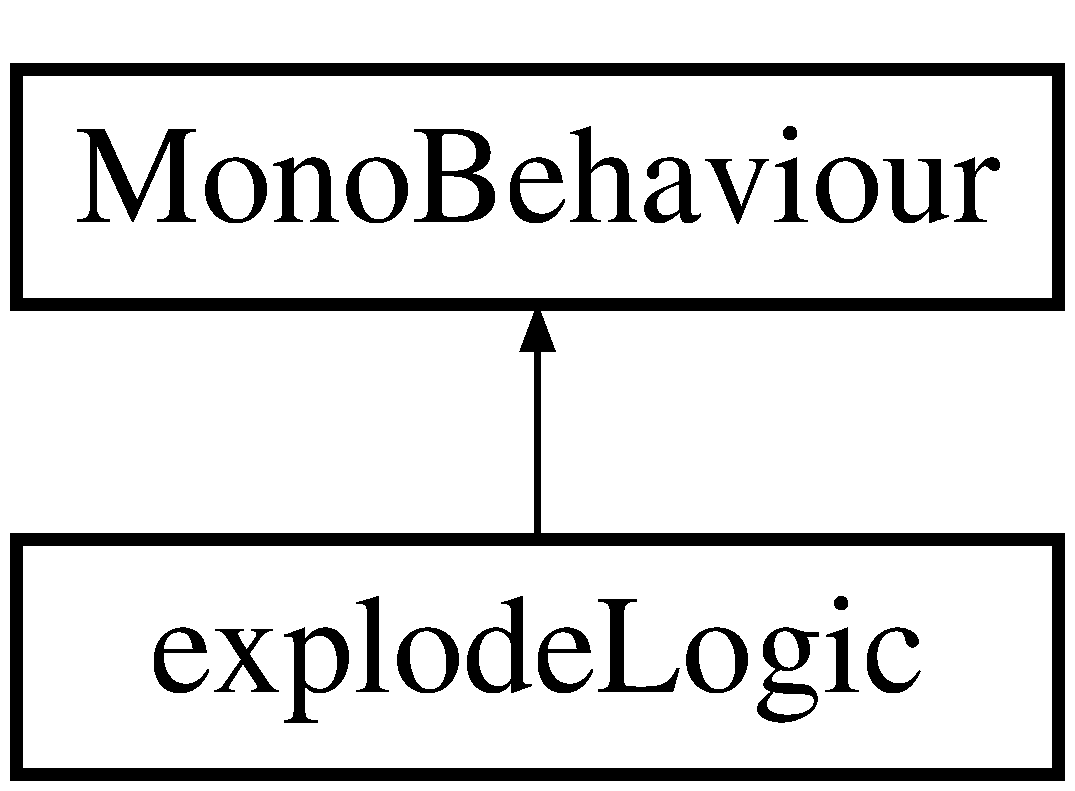
\includegraphics[height=2.000000cm]{classexplode_logic}
\end{center}
\end{figure}
\subsection*{Public Member Functions}
\begin{DoxyCompactItemize}
\item 
void \hyperlink{classexplode_logic_a9c58298b6ca7bba45997d736618c6aca}{On\+Trigger\+Enter2D} (Collider2D other)
\end{DoxyCompactItemize}


\subsection{Member Function Documentation}
\mbox{\Hypertarget{classexplode_logic_a9c58298b6ca7bba45997d736618c6aca}\label{classexplode_logic_a9c58298b6ca7bba45997d736618c6aca}} 
\index{explode\+Logic@{explode\+Logic}!On\+Trigger\+Enter2D@{On\+Trigger\+Enter2D}}
\index{On\+Trigger\+Enter2D@{On\+Trigger\+Enter2D}!explode\+Logic@{explode\+Logic}}
\subsubsection{\texorpdfstring{On\+Trigger\+Enter2\+D()}{OnTriggerEnter2D()}}
{\footnotesize\ttfamily void explode\+Logic.\+On\+Trigger\+Enter2D (\begin{DoxyParamCaption}\item[{Collider2D}]{other }\end{DoxyParamCaption})}



The documentation for this class was generated from the following file\+:\begin{DoxyCompactItemize}
\item 
/\+Users/kwanholloway/git/5001\+Project/\+Game\+Project/\+Assets/\+Scripts/\+Game\+Logic/\hyperlink{explode_logic_8cs}{explode\+Logic.\+cs}\end{DoxyCompactItemize}

\hypertarget{class_final_puzzle_completion_check}{}\section{Final\+Puzzle\+Completion\+Check Class Reference}
\label{class_final_puzzle_completion_check}\index{Final\+Puzzle\+Completion\+Check@{Final\+Puzzle\+Completion\+Check}}
Inheritance diagram for Final\+Puzzle\+Completion\+Check\+:\begin{figure}[H]
\begin{center}
\leavevmode
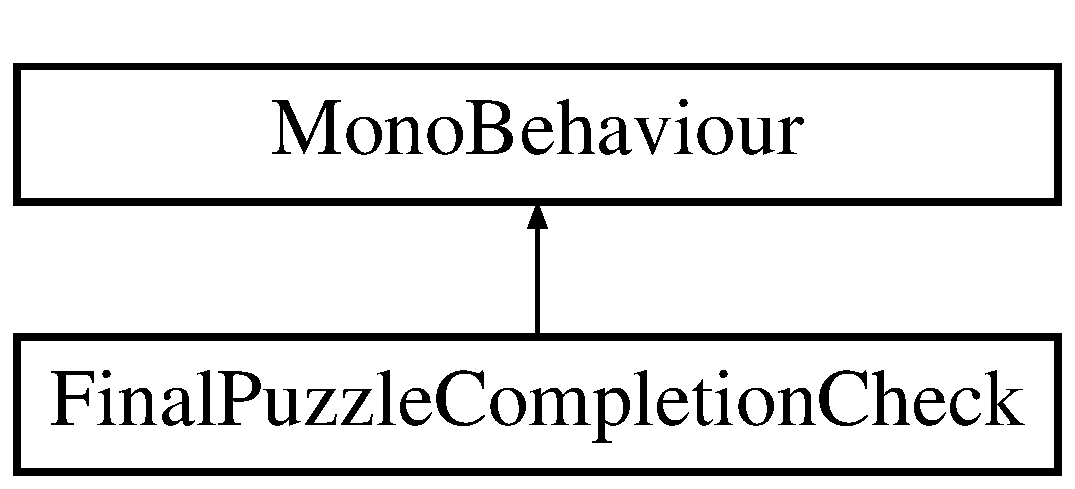
\includegraphics[height=2.000000cm]{class_final_puzzle_completion_check}
\end{center}
\end{figure}
\subsection*{Public Member Functions}
\begin{DoxyCompactItemize}
\item 
void \hyperlink{class_final_puzzle_completion_check_afa55397d4f336e82c9767986f9312860}{reset\+Puzzle} ()
\item 
void \hyperlink{class_final_puzzle_completion_check_a47383ae7a03f939730d8c5290e92c0cc}{reset\+Check\+Values} ()
\item 
void \hyperlink{class_final_puzzle_completion_check_a2cd4702593ffbf8357cc0eddf24f553e}{activate\+Elevator} ()
\item 
void \hyperlink{class_final_puzzle_completion_check_add677a80884393ac52213eeb22615f4b}{reset\+Slots} ()
\item 
void \hyperlink{class_final_puzzle_completion_check_ac703da00c5cf3cc8dfad601b1961a9a3}{reset\+Tiles} ()
\item 
void \hyperlink{class_final_puzzle_completion_check_a74ba145de0f91eec81cdf77c6a0ed104}{reset\+Active} ()
\item 
bool \hyperlink{class_final_puzzle_completion_check_afa978714de4b54e9af76c01419ed5909}{check\+Input\+Success} ()
\item 
bool \hyperlink{class_final_puzzle_completion_check_aadb51258547c069a6597074951578423}{check\+Input\+Name} ()
\end{DoxyCompactItemize}
\subsection*{Public Attributes}
\begin{DoxyCompactItemize}
\item 
Game\+Object \mbox{[}$\,$\mbox{]} \hyperlink{class_final_puzzle_completion_check_afeeb6c56f30c0f636803891a7dd3f53a}{check\+Slots}
\begin{DoxyCompactList}\small\item\em manually set in inspector, slots to be filled by tiles \end{DoxyCompactList}\item 
Game\+Object \mbox{[}$\,$\mbox{]} \hyperlink{class_final_puzzle_completion_check_ab25b67e68be39b9459b6b0f6aa8429b9}{array\+Tiles}
\begin{DoxyCompactList}\small\item\em the tiles that will be dragged \end{DoxyCompactList}\item 
Game\+Object \mbox{[}$\,$\mbox{]} \hyperlink{class_final_puzzle_completion_check_a778ec2e2631b81862469ef127e2799db}{replacement\+Tiles}
\begin{DoxyCompactList}\small\item\em The replacement tiles that go into the slots \end{DoxyCompactList}\item 
Text \hyperlink{class_final_puzzle_completion_check_adf7b1db99726b1744800ff53f9fd32dd}{error\+Message}
\begin{DoxyCompactList}\small\item\em error message for the canvas \end{DoxyCompactList}\item 
bool \hyperlink{class_final_puzzle_completion_check_ad5b37fa48358e0e302c312e015875b4d}{puzzle\+Finished}
\end{DoxyCompactItemize}


\subsection{Detailed Description}
Checks the respective challenge and makes changes to the game if the user is correct or not Challenge\+: Final challenge 2 

\subsection{Member Function Documentation}
\mbox{\Hypertarget{class_final_puzzle_completion_check_a2cd4702593ffbf8357cc0eddf24f553e}\label{class_final_puzzle_completion_check_a2cd4702593ffbf8357cc0eddf24f553e}} 
\index{Final\+Puzzle\+Completion\+Check@{Final\+Puzzle\+Completion\+Check}!activate\+Elevator@{activate\+Elevator}}
\index{activate\+Elevator@{activate\+Elevator}!Final\+Puzzle\+Completion\+Check@{Final\+Puzzle\+Completion\+Check}}
\subsubsection{\texorpdfstring{activate\+Elevator()}{activateElevator()}}
{\footnotesize\ttfamily void Final\+Puzzle\+Completion\+Check.\+activate\+Elevator (\begin{DoxyParamCaption}{ }\end{DoxyParamCaption})}

\mbox{\Hypertarget{class_final_puzzle_completion_check_aadb51258547c069a6597074951578423}\label{class_final_puzzle_completion_check_aadb51258547c069a6597074951578423}} 
\index{Final\+Puzzle\+Completion\+Check@{Final\+Puzzle\+Completion\+Check}!check\+Input\+Name@{check\+Input\+Name}}
\index{check\+Input\+Name@{check\+Input\+Name}!Final\+Puzzle\+Completion\+Check@{Final\+Puzzle\+Completion\+Check}}
\subsubsection{\texorpdfstring{check\+Input\+Name()}{checkInputName()}}
{\footnotesize\ttfamily bool Final\+Puzzle\+Completion\+Check.\+check\+Input\+Name (\begin{DoxyParamCaption}{ }\end{DoxyParamCaption})}

\mbox{\Hypertarget{class_final_puzzle_completion_check_afa978714de4b54e9af76c01419ed5909}\label{class_final_puzzle_completion_check_afa978714de4b54e9af76c01419ed5909}} 
\index{Final\+Puzzle\+Completion\+Check@{Final\+Puzzle\+Completion\+Check}!check\+Input\+Success@{check\+Input\+Success}}
\index{check\+Input\+Success@{check\+Input\+Success}!Final\+Puzzle\+Completion\+Check@{Final\+Puzzle\+Completion\+Check}}
\subsubsection{\texorpdfstring{check\+Input\+Success()}{checkInputSuccess()}}
{\footnotesize\ttfamily bool Final\+Puzzle\+Completion\+Check.\+check\+Input\+Success (\begin{DoxyParamCaption}{ }\end{DoxyParamCaption})}

\mbox{\Hypertarget{class_final_puzzle_completion_check_a74ba145de0f91eec81cdf77c6a0ed104}\label{class_final_puzzle_completion_check_a74ba145de0f91eec81cdf77c6a0ed104}} 
\index{Final\+Puzzle\+Completion\+Check@{Final\+Puzzle\+Completion\+Check}!reset\+Active@{reset\+Active}}
\index{reset\+Active@{reset\+Active}!Final\+Puzzle\+Completion\+Check@{Final\+Puzzle\+Completion\+Check}}
\subsubsection{\texorpdfstring{reset\+Active()}{resetActive()}}
{\footnotesize\ttfamily void Final\+Puzzle\+Completion\+Check.\+reset\+Active (\begin{DoxyParamCaption}{ }\end{DoxyParamCaption})}

\mbox{\Hypertarget{class_final_puzzle_completion_check_a47383ae7a03f939730d8c5290e92c0cc}\label{class_final_puzzle_completion_check_a47383ae7a03f939730d8c5290e92c0cc}} 
\index{Final\+Puzzle\+Completion\+Check@{Final\+Puzzle\+Completion\+Check}!reset\+Check\+Values@{reset\+Check\+Values}}
\index{reset\+Check\+Values@{reset\+Check\+Values}!Final\+Puzzle\+Completion\+Check@{Final\+Puzzle\+Completion\+Check}}
\subsubsection{\texorpdfstring{reset\+Check\+Values()}{resetCheckValues()}}
{\footnotesize\ttfamily void Final\+Puzzle\+Completion\+Check.\+reset\+Check\+Values (\begin{DoxyParamCaption}{ }\end{DoxyParamCaption})}

\mbox{\Hypertarget{class_final_puzzle_completion_check_afa55397d4f336e82c9767986f9312860}\label{class_final_puzzle_completion_check_afa55397d4f336e82c9767986f9312860}} 
\index{Final\+Puzzle\+Completion\+Check@{Final\+Puzzle\+Completion\+Check}!reset\+Puzzle@{reset\+Puzzle}}
\index{reset\+Puzzle@{reset\+Puzzle}!Final\+Puzzle\+Completion\+Check@{Final\+Puzzle\+Completion\+Check}}
\subsubsection{\texorpdfstring{reset\+Puzzle()}{resetPuzzle()}}
{\footnotesize\ttfamily void Final\+Puzzle\+Completion\+Check.\+reset\+Puzzle (\begin{DoxyParamCaption}{ }\end{DoxyParamCaption})}

Resets the puzzle Resets the Tiles, slots, check values, camera flag and error message \mbox{\Hypertarget{class_final_puzzle_completion_check_add677a80884393ac52213eeb22615f4b}\label{class_final_puzzle_completion_check_add677a80884393ac52213eeb22615f4b}} 
\index{Final\+Puzzle\+Completion\+Check@{Final\+Puzzle\+Completion\+Check}!reset\+Slots@{reset\+Slots}}
\index{reset\+Slots@{reset\+Slots}!Final\+Puzzle\+Completion\+Check@{Final\+Puzzle\+Completion\+Check}}
\subsubsection{\texorpdfstring{reset\+Slots()}{resetSlots()}}
{\footnotesize\ttfamily void Final\+Puzzle\+Completion\+Check.\+reset\+Slots (\begin{DoxyParamCaption}{ }\end{DoxyParamCaption})}

\mbox{\Hypertarget{class_final_puzzle_completion_check_ac703da00c5cf3cc8dfad601b1961a9a3}\label{class_final_puzzle_completion_check_ac703da00c5cf3cc8dfad601b1961a9a3}} 
\index{Final\+Puzzle\+Completion\+Check@{Final\+Puzzle\+Completion\+Check}!reset\+Tiles@{reset\+Tiles}}
\index{reset\+Tiles@{reset\+Tiles}!Final\+Puzzle\+Completion\+Check@{Final\+Puzzle\+Completion\+Check}}
\subsubsection{\texorpdfstring{reset\+Tiles()}{resetTiles()}}
{\footnotesize\ttfamily void Final\+Puzzle\+Completion\+Check.\+reset\+Tiles (\begin{DoxyParamCaption}{ }\end{DoxyParamCaption})}



\subsection{Member Data Documentation}
\mbox{\Hypertarget{class_final_puzzle_completion_check_ab25b67e68be39b9459b6b0f6aa8429b9}\label{class_final_puzzle_completion_check_ab25b67e68be39b9459b6b0f6aa8429b9}} 
\index{Final\+Puzzle\+Completion\+Check@{Final\+Puzzle\+Completion\+Check}!array\+Tiles@{array\+Tiles}}
\index{array\+Tiles@{array\+Tiles}!Final\+Puzzle\+Completion\+Check@{Final\+Puzzle\+Completion\+Check}}
\subsubsection{\texorpdfstring{array\+Tiles}{arrayTiles}}
{\footnotesize\ttfamily Game\+Object \mbox{[}$\,$\mbox{]} Final\+Puzzle\+Completion\+Check.\+array\+Tiles}



the tiles that will be dragged 

\mbox{\Hypertarget{class_final_puzzle_completion_check_afeeb6c56f30c0f636803891a7dd3f53a}\label{class_final_puzzle_completion_check_afeeb6c56f30c0f636803891a7dd3f53a}} 
\index{Final\+Puzzle\+Completion\+Check@{Final\+Puzzle\+Completion\+Check}!check\+Slots@{check\+Slots}}
\index{check\+Slots@{check\+Slots}!Final\+Puzzle\+Completion\+Check@{Final\+Puzzle\+Completion\+Check}}
\subsubsection{\texorpdfstring{check\+Slots}{checkSlots}}
{\footnotesize\ttfamily Game\+Object \mbox{[}$\,$\mbox{]} Final\+Puzzle\+Completion\+Check.\+check\+Slots}



manually set in inspector, slots to be filled by tiles 

\mbox{\Hypertarget{class_final_puzzle_completion_check_adf7b1db99726b1744800ff53f9fd32dd}\label{class_final_puzzle_completion_check_adf7b1db99726b1744800ff53f9fd32dd}} 
\index{Final\+Puzzle\+Completion\+Check@{Final\+Puzzle\+Completion\+Check}!error\+Message@{error\+Message}}
\index{error\+Message@{error\+Message}!Final\+Puzzle\+Completion\+Check@{Final\+Puzzle\+Completion\+Check}}
\subsubsection{\texorpdfstring{error\+Message}{errorMessage}}
{\footnotesize\ttfamily Text Final\+Puzzle\+Completion\+Check.\+error\+Message}



error message for the canvas 

\mbox{\Hypertarget{class_final_puzzle_completion_check_ad5b37fa48358e0e302c312e015875b4d}\label{class_final_puzzle_completion_check_ad5b37fa48358e0e302c312e015875b4d}} 
\index{Final\+Puzzle\+Completion\+Check@{Final\+Puzzle\+Completion\+Check}!puzzle\+Finished@{puzzle\+Finished}}
\index{puzzle\+Finished@{puzzle\+Finished}!Final\+Puzzle\+Completion\+Check@{Final\+Puzzle\+Completion\+Check}}
\subsubsection{\texorpdfstring{puzzle\+Finished}{puzzleFinished}}
{\footnotesize\ttfamily bool Final\+Puzzle\+Completion\+Check.\+puzzle\+Finished}

\mbox{\Hypertarget{class_final_puzzle_completion_check_a778ec2e2631b81862469ef127e2799db}\label{class_final_puzzle_completion_check_a778ec2e2631b81862469ef127e2799db}} 
\index{Final\+Puzzle\+Completion\+Check@{Final\+Puzzle\+Completion\+Check}!replacement\+Tiles@{replacement\+Tiles}}
\index{replacement\+Tiles@{replacement\+Tiles}!Final\+Puzzle\+Completion\+Check@{Final\+Puzzle\+Completion\+Check}}
\subsubsection{\texorpdfstring{replacement\+Tiles}{replacementTiles}}
{\footnotesize\ttfamily Game\+Object \mbox{[}$\,$\mbox{]} Final\+Puzzle\+Completion\+Check.\+replacement\+Tiles}



The replacement tiles that go into the slots 



The documentation for this class was generated from the following file\+:\begin{DoxyCompactItemize}
\item 
/\+Users/kwanholloway/git/5001\+Project/\+Game\+Project/\+Assets/\+Scripts/\+Puzzle\+Logic/\+Final\+Level/\hyperlink{_final_puzzle_completion_check_8cs}{Final\+Puzzle\+Completion\+Check.\+cs}\end{DoxyCompactItemize}

\hypertarget{class_final_room_door}{}\section{Final\+Room\+Door Class Reference}
\label{class_final_room_door}\index{Final\+Room\+Door@{Final\+Room\+Door}}
Inheritance diagram for Final\+Room\+Door\+:\begin{figure}[H]
\begin{center}
\leavevmode
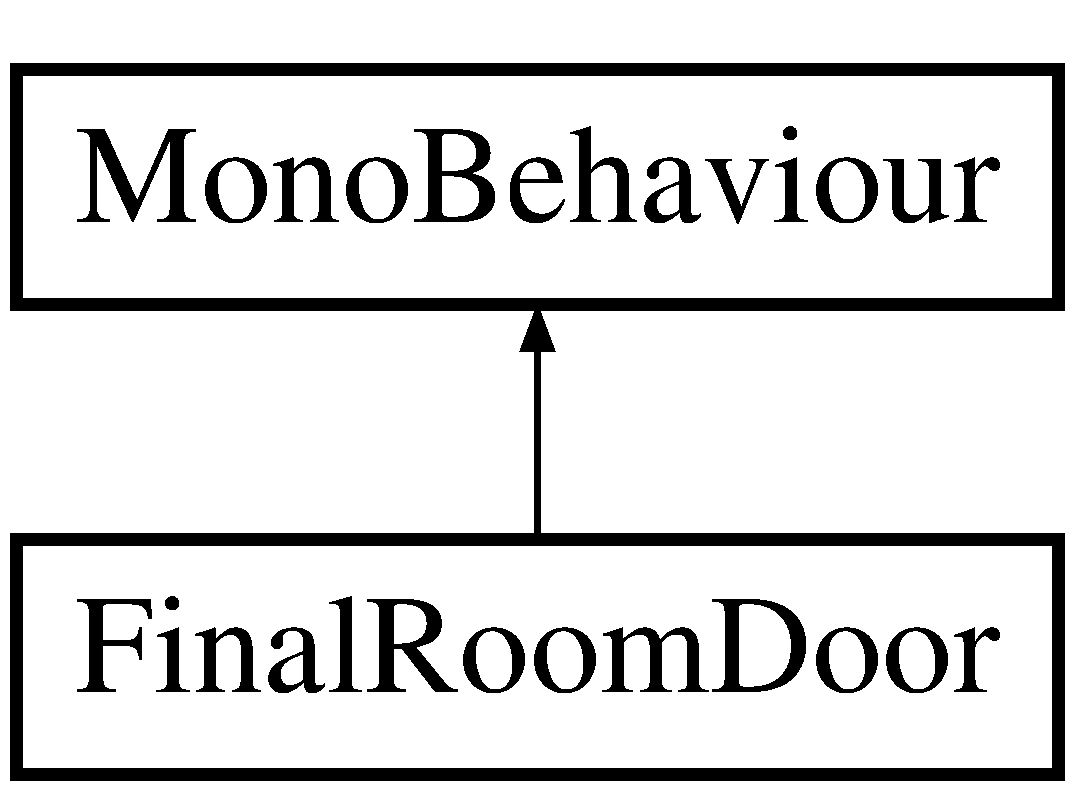
\includegraphics[height=2.000000cm]{class_final_room_door}
\end{center}
\end{figure}
\subsection*{Public Attributes}
\begin{DoxyCompactItemize}
\item 
Game\+Object \hyperlink{class_final_room_door_a60613bd2f5b603777262b96ed07e87d0}{door\+One}
\end{DoxyCompactItemize}


\subsection{Detailed Description}
Manages the door that clocks the fnial level in the Hub L\+Evel of the game 

\subsection{Member Data Documentation}
\mbox{\Hypertarget{class_final_room_door_a60613bd2f5b603777262b96ed07e87d0}\label{class_final_room_door_a60613bd2f5b603777262b96ed07e87d0}} 
\index{Final\+Room\+Door@{Final\+Room\+Door}!door\+One@{door\+One}}
\index{door\+One@{door\+One}!Final\+Room\+Door@{Final\+Room\+Door}}
\subsubsection{\texorpdfstring{door\+One}{doorOne}}
{\footnotesize\ttfamily Game\+Object Final\+Room\+Door.\+door\+One}



The documentation for this class was generated from the following file\+:\begin{DoxyCompactItemize}
\item 
/\+Users/kwanholloway/git/5001\+Project/\+Game\+Project/\+Assets/\+Scripts/\+Game\+Logic/\hyperlink{_final_room_door_8cs}{Final\+Room\+Door.\+cs}\end{DoxyCompactItemize}

\hypertarget{class_for_loop_desk_top_interaction}{}\section{For\+Loop\+Desk\+Top\+Interaction Class Reference}
\label{class_for_loop_desk_top_interaction}\index{For\+Loop\+Desk\+Top\+Interaction@{For\+Loop\+Desk\+Top\+Interaction}}
Inheritance diagram for For\+Loop\+Desk\+Top\+Interaction\+:\begin{figure}[H]
\begin{center}
\leavevmode
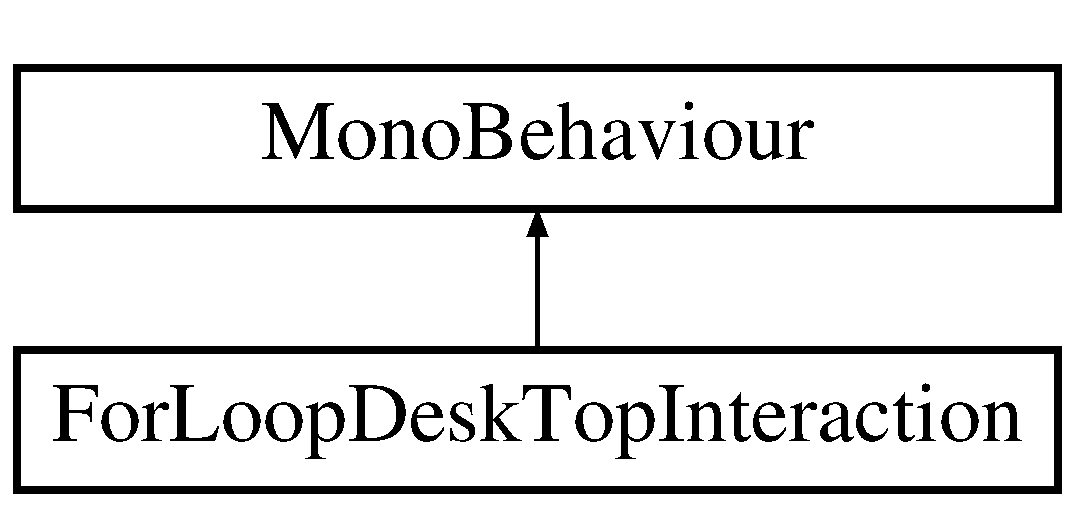
\includegraphics[height=2.000000cm]{class_for_loop_desk_top_interaction}
\end{center}
\end{figure}
\subsection*{Public Attributes}
\begin{DoxyCompactItemize}
\item 
Text \hyperlink{class_for_loop_desk_top_interaction_a333c1f48a76d8e74cad5e01b1cad3929}{prompt}
\end{DoxyCompactItemize}


\subsection{Member Data Documentation}
\mbox{\Hypertarget{class_for_loop_desk_top_interaction_a333c1f48a76d8e74cad5e01b1cad3929}\label{class_for_loop_desk_top_interaction_a333c1f48a76d8e74cad5e01b1cad3929}} 
\index{For\+Loop\+Desk\+Top\+Interaction@{For\+Loop\+Desk\+Top\+Interaction}!prompt@{prompt}}
\index{prompt@{prompt}!For\+Loop\+Desk\+Top\+Interaction@{For\+Loop\+Desk\+Top\+Interaction}}
\subsubsection{\texorpdfstring{prompt}{prompt}}
{\footnotesize\ttfamily Text For\+Loop\+Desk\+Top\+Interaction.\+prompt}



The documentation for this class was generated from the following file\+:\begin{DoxyCompactItemize}
\item 
/\+Users/kwanholloway/git/5001\+Project/\+Game\+Project/\+Assets/\+Scripts/\+Game\+Logic/\hyperlink{_for_loop_desk_top_interaction_8cs}{For\+Loop\+Desk\+Top\+Interaction.\+cs}\end{DoxyCompactItemize}

\hypertarget{class_game_buttons}{}\section{Game\+Buttons Class Reference}
\label{class_game_buttons}\index{Game\+Buttons@{Game\+Buttons}}
Inheritance diagram for Game\+Buttons\+:\begin{figure}[H]
\begin{center}
\leavevmode
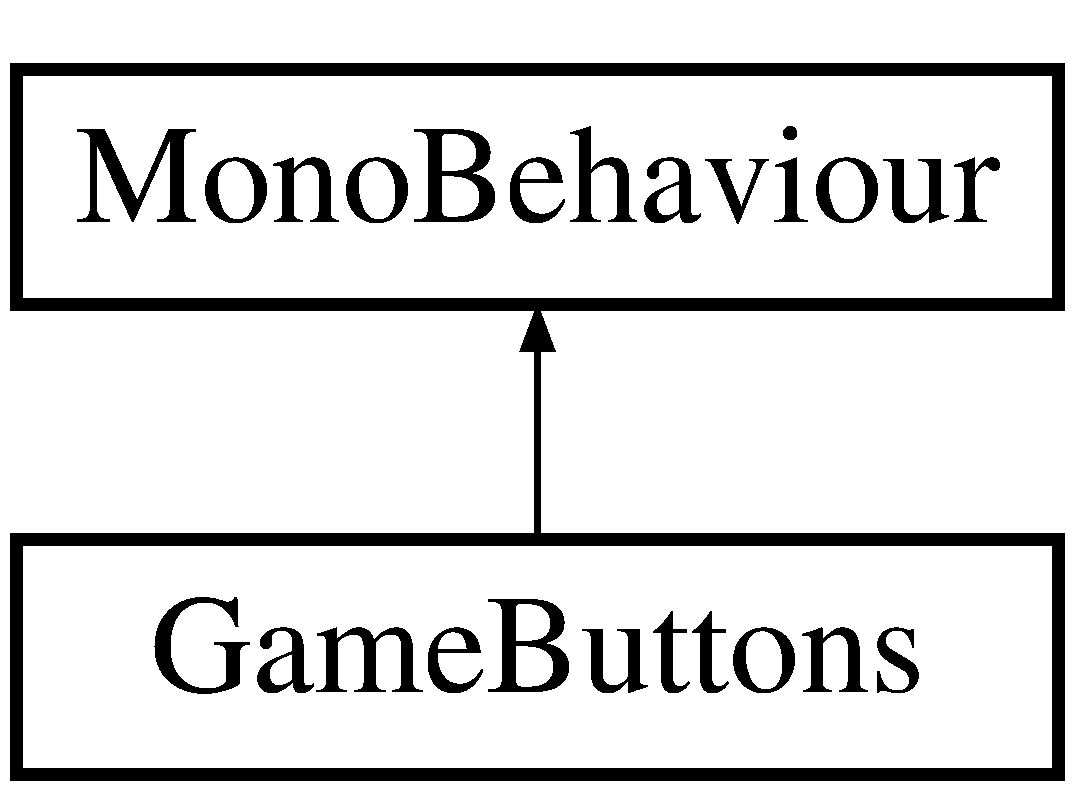
\includegraphics[height=2.000000cm]{class_game_buttons}
\end{center}
\end{figure}
\subsection*{Public Member Functions}
\begin{DoxyCompactItemize}
\item 
void \hyperlink{class_game_buttons_aa6666b810a7a0caff54b55d473be24c9}{Pause\+Game} ()
\item 
void \hyperlink{class_game_buttons_af088dcf9d9b5393c1c22bf2122cffe35}{Resume\+Game} ()
\item 
void \hyperlink{class_game_buttons_aa55857210a186acda2b262d2cab348b8}{Clear\+Word\+Display} ()
\begin{DoxyCompactList}\small\item\em Clears the message\+Panel and it\textquotesingle{}s Word\+Displayer. \end{DoxyCompactList}\item 
void \hyperlink{class_game_buttons_a64856a3c989ce3d14db961766db49425}{Menu} ()
\item 
void \hyperlink{class_game_buttons_a53eb5843078798e6617647ae83bfbc1e}{Go\+To\+Introduction} ()
\item 
void \hyperlink{class_game_buttons_ac91982c8a1409e977ceb47220fd7112a}{Go\+To\+Instructions} ()
\item 
void \hyperlink{class_game_buttons_acfb2c2af597071c65abe2535199bf5d9}{Start\+Game} ()
\item 
void \hyperlink{class_game_buttons_aa24ecd9e57ec9e74b94d2e974655c630}{Return\+To\+Title} ()
\item 
void \hyperlink{class_game_buttons_a0bf79754f2ddf3fcc4059e9179b74024}{Quit\+Game} ()
\item 
void \hyperlink{class_game_buttons_a38fd8fbd392123bfa94d3a291afd725e}{Return\+To\+Prev\+Scene} ()
\item 
void \hyperlink{class_game_buttons_a1ca7b15fb784ed277bc107613d95606d}{help\+Screen\+Toggle} ()
\item 
void \hyperlink{class_game_buttons_a2a81335687a2eb013f83fccf7394f57d}{help\+Toggle\+Off} ()
\end{DoxyCompactItemize}
\subsection*{Public Attributes}
\begin{DoxyCompactItemize}
\item 
Camera \hyperlink{class_game_buttons_a2209c4c549e16c9c815b1c0a3a15bbbd}{help\+Camera}
\item 
Analytics\+By\+Level \hyperlink{class_game_buttons_a1d1a3181b45c9bd292fa2490acb742c2}{level\+Analytics}
\end{DoxyCompactItemize}


\subsection{Detailed Description}
Manages various game buttons that are uses within the canvas, among other objects. Provides functionality for pausing, quiting the game. Also toggling help pages and more. 

\subsection{Member Function Documentation}
\mbox{\Hypertarget{class_game_buttons_aa55857210a186acda2b262d2cab348b8}\label{class_game_buttons_aa55857210a186acda2b262d2cab348b8}} 
\index{Game\+Buttons@{Game\+Buttons}!Clear\+Word\+Display@{Clear\+Word\+Display}}
\index{Clear\+Word\+Display@{Clear\+Word\+Display}!Game\+Buttons@{Game\+Buttons}}
\subsubsection{\texorpdfstring{Clear\+Word\+Display()}{ClearWordDisplay()}}
{\footnotesize\ttfamily void Game\+Buttons.\+Clear\+Word\+Display (\begin{DoxyParamCaption}{ }\end{DoxyParamCaption})}



Clears the message\+Panel and it\textquotesingle{}s Word\+Displayer. 

\mbox{\Hypertarget{class_game_buttons_ac91982c8a1409e977ceb47220fd7112a}\label{class_game_buttons_ac91982c8a1409e977ceb47220fd7112a}} 
\index{Game\+Buttons@{Game\+Buttons}!Go\+To\+Instructions@{Go\+To\+Instructions}}
\index{Go\+To\+Instructions@{Go\+To\+Instructions}!Game\+Buttons@{Game\+Buttons}}
\subsubsection{\texorpdfstring{Go\+To\+Instructions()}{GoToInstructions()}}
{\footnotesize\ttfamily void Game\+Buttons.\+Go\+To\+Instructions (\begin{DoxyParamCaption}{ }\end{DoxyParamCaption})}

\mbox{\Hypertarget{class_game_buttons_a53eb5843078798e6617647ae83bfbc1e}\label{class_game_buttons_a53eb5843078798e6617647ae83bfbc1e}} 
\index{Game\+Buttons@{Game\+Buttons}!Go\+To\+Introduction@{Go\+To\+Introduction}}
\index{Go\+To\+Introduction@{Go\+To\+Introduction}!Game\+Buttons@{Game\+Buttons}}
\subsubsection{\texorpdfstring{Go\+To\+Introduction()}{GoToIntroduction()}}
{\footnotesize\ttfamily void Game\+Buttons.\+Go\+To\+Introduction (\begin{DoxyParamCaption}{ }\end{DoxyParamCaption})}

\mbox{\Hypertarget{class_game_buttons_a1ca7b15fb784ed277bc107613d95606d}\label{class_game_buttons_a1ca7b15fb784ed277bc107613d95606d}} 
\index{Game\+Buttons@{Game\+Buttons}!help\+Screen\+Toggle@{help\+Screen\+Toggle}}
\index{help\+Screen\+Toggle@{help\+Screen\+Toggle}!Game\+Buttons@{Game\+Buttons}}
\subsubsection{\texorpdfstring{help\+Screen\+Toggle()}{helpScreenToggle()}}
{\footnotesize\ttfamily void Game\+Buttons.\+help\+Screen\+Toggle (\begin{DoxyParamCaption}{ }\end{DoxyParamCaption})}

Toggles the help screen by finding the right camera and toggling \mbox{\Hypertarget{class_game_buttons_a2a81335687a2eb013f83fccf7394f57d}\label{class_game_buttons_a2a81335687a2eb013f83fccf7394f57d}} 
\index{Game\+Buttons@{Game\+Buttons}!help\+Toggle\+Off@{help\+Toggle\+Off}}
\index{help\+Toggle\+Off@{help\+Toggle\+Off}!Game\+Buttons@{Game\+Buttons}}
\subsubsection{\texorpdfstring{help\+Toggle\+Off()}{helpToggleOff()}}
{\footnotesize\ttfamily void Game\+Buttons.\+help\+Toggle\+Off (\begin{DoxyParamCaption}{ }\end{DoxyParamCaption})}

\mbox{\Hypertarget{class_game_buttons_a64856a3c989ce3d14db961766db49425}\label{class_game_buttons_a64856a3c989ce3d14db961766db49425}} 
\index{Game\+Buttons@{Game\+Buttons}!Menu@{Menu}}
\index{Menu@{Menu}!Game\+Buttons@{Game\+Buttons}}
\subsubsection{\texorpdfstring{Menu()}{Menu()}}
{\footnotesize\ttfamily void Game\+Buttons.\+Menu (\begin{DoxyParamCaption}{ }\end{DoxyParamCaption})}

\mbox{\Hypertarget{class_game_buttons_aa6666b810a7a0caff54b55d473be24c9}\label{class_game_buttons_aa6666b810a7a0caff54b55d473be24c9}} 
\index{Game\+Buttons@{Game\+Buttons}!Pause\+Game@{Pause\+Game}}
\index{Pause\+Game@{Pause\+Game}!Game\+Buttons@{Game\+Buttons}}
\subsubsection{\texorpdfstring{Pause\+Game()}{PauseGame()}}
{\footnotesize\ttfamily void Game\+Buttons.\+Pause\+Game (\begin{DoxyParamCaption}{ }\end{DoxyParamCaption})}

\mbox{\Hypertarget{class_game_buttons_a0bf79754f2ddf3fcc4059e9179b74024}\label{class_game_buttons_a0bf79754f2ddf3fcc4059e9179b74024}} 
\index{Game\+Buttons@{Game\+Buttons}!Quit\+Game@{Quit\+Game}}
\index{Quit\+Game@{Quit\+Game}!Game\+Buttons@{Game\+Buttons}}
\subsubsection{\texorpdfstring{Quit\+Game()}{QuitGame()}}
{\footnotesize\ttfamily void Game\+Buttons.\+Quit\+Game (\begin{DoxyParamCaption}{ }\end{DoxyParamCaption})}

\mbox{\Hypertarget{class_game_buttons_af088dcf9d9b5393c1c22bf2122cffe35}\label{class_game_buttons_af088dcf9d9b5393c1c22bf2122cffe35}} 
\index{Game\+Buttons@{Game\+Buttons}!Resume\+Game@{Resume\+Game}}
\index{Resume\+Game@{Resume\+Game}!Game\+Buttons@{Game\+Buttons}}
\subsubsection{\texorpdfstring{Resume\+Game()}{ResumeGame()}}
{\footnotesize\ttfamily void Game\+Buttons.\+Resume\+Game (\begin{DoxyParamCaption}{ }\end{DoxyParamCaption})}

\mbox{\Hypertarget{class_game_buttons_a38fd8fbd392123bfa94d3a291afd725e}\label{class_game_buttons_a38fd8fbd392123bfa94d3a291afd725e}} 
\index{Game\+Buttons@{Game\+Buttons}!Return\+To\+Prev\+Scene@{Return\+To\+Prev\+Scene}}
\index{Return\+To\+Prev\+Scene@{Return\+To\+Prev\+Scene}!Game\+Buttons@{Game\+Buttons}}
\subsubsection{\texorpdfstring{Return\+To\+Prev\+Scene()}{ReturnToPrevScene()}}
{\footnotesize\ttfamily void Game\+Buttons.\+Return\+To\+Prev\+Scene (\begin{DoxyParamCaption}{ }\end{DoxyParamCaption})}

\mbox{\Hypertarget{class_game_buttons_aa24ecd9e57ec9e74b94d2e974655c630}\label{class_game_buttons_aa24ecd9e57ec9e74b94d2e974655c630}} 
\index{Game\+Buttons@{Game\+Buttons}!Return\+To\+Title@{Return\+To\+Title}}
\index{Return\+To\+Title@{Return\+To\+Title}!Game\+Buttons@{Game\+Buttons}}
\subsubsection{\texorpdfstring{Return\+To\+Title()}{ReturnToTitle()}}
{\footnotesize\ttfamily void Game\+Buttons.\+Return\+To\+Title (\begin{DoxyParamCaption}{ }\end{DoxyParamCaption})}

\mbox{\Hypertarget{class_game_buttons_acfb2c2af597071c65abe2535199bf5d9}\label{class_game_buttons_acfb2c2af597071c65abe2535199bf5d9}} 
\index{Game\+Buttons@{Game\+Buttons}!Start\+Game@{Start\+Game}}
\index{Start\+Game@{Start\+Game}!Game\+Buttons@{Game\+Buttons}}
\subsubsection{\texorpdfstring{Start\+Game()}{StartGame()}}
{\footnotesize\ttfamily void Game\+Buttons.\+Start\+Game (\begin{DoxyParamCaption}{ }\end{DoxyParamCaption})}



\subsection{Member Data Documentation}
\mbox{\Hypertarget{class_game_buttons_a2209c4c549e16c9c815b1c0a3a15bbbd}\label{class_game_buttons_a2209c4c549e16c9c815b1c0a3a15bbbd}} 
\index{Game\+Buttons@{Game\+Buttons}!help\+Camera@{help\+Camera}}
\index{help\+Camera@{help\+Camera}!Game\+Buttons@{Game\+Buttons}}
\subsubsection{\texorpdfstring{help\+Camera}{helpCamera}}
{\footnotesize\ttfamily Camera Game\+Buttons.\+help\+Camera}

\mbox{\Hypertarget{class_game_buttons_a1d1a3181b45c9bd292fa2490acb742c2}\label{class_game_buttons_a1d1a3181b45c9bd292fa2490acb742c2}} 
\index{Game\+Buttons@{Game\+Buttons}!level\+Analytics@{level\+Analytics}}
\index{level\+Analytics@{level\+Analytics}!Game\+Buttons@{Game\+Buttons}}
\subsubsection{\texorpdfstring{level\+Analytics}{levelAnalytics}}
{\footnotesize\ttfamily Analytics\+By\+Level Game\+Buttons.\+level\+Analytics}



The documentation for this class was generated from the following file\+:\begin{DoxyCompactItemize}
\item 
/\+Users/kwanholloway/git/5001\+Project/\+Game\+Project/\+Assets/\+Scripts/\+Menu\+Nav\+Scripts/\hyperlink{_game_buttons_8cs}{Game\+Buttons.\+cs}\end{DoxyCompactItemize}

\hypertarget{class_global_controller}{}\section{Global\+Controller Class Reference}
\label{class_global_controller}\index{Global\+Controller@{Global\+Controller}}
Inheritance diagram for Global\+Controller\+:\begin{figure}[H]
\begin{center}
\leavevmode
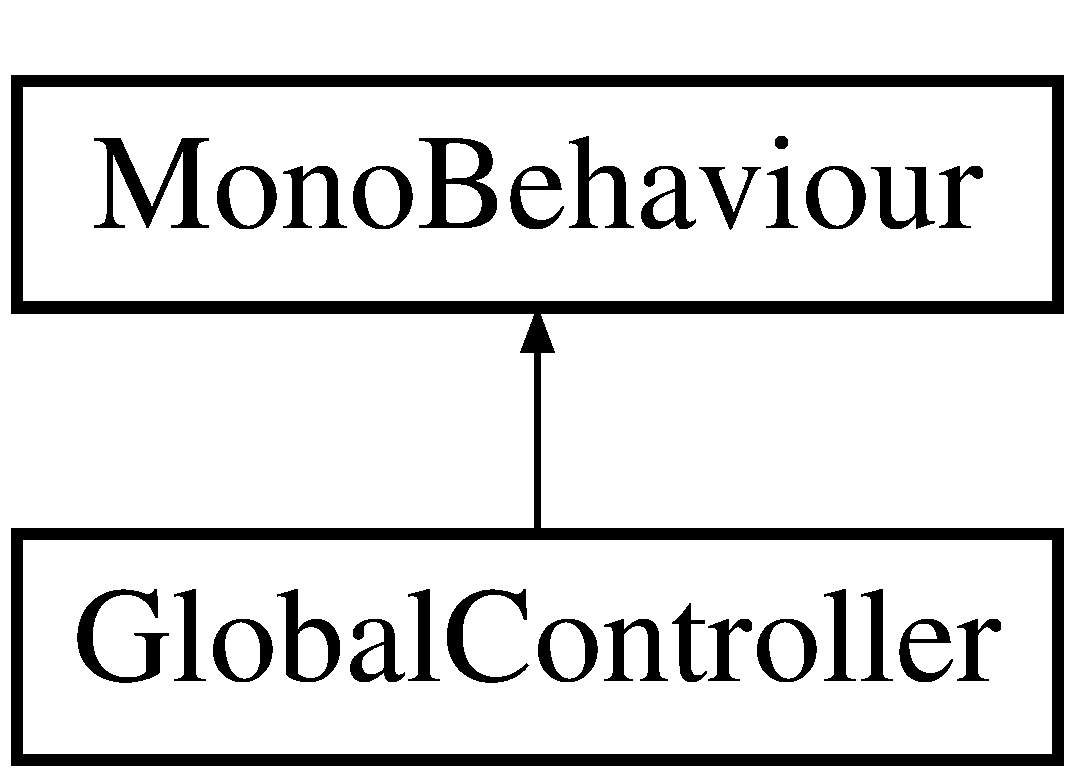
\includegraphics[height=2.000000cm]{class_global_controller}
\end{center}
\end{figure}
\subsection*{Public Member Functions}
\begin{DoxyCompactItemize}
\item 
void \hyperlink{class_global_controller_a5a71c2551eef6be2304110c96a31cb55}{save\+Player\+Pos} ()
\begin{DoxyCompactList}\small\item\em save the players position for use between scenes \end{DoxyCompactList}\item 
void \hyperlink{class_global_controller_a3424caeaad35cc27c958d453ac7586fc}{set\+Player\+Pos} ()
\begin{DoxyCompactList}\small\item\em sets the players position when returning to scene \end{DoxyCompactList}\item 
void \hyperlink{class_global_controller_af0ae9de1725a09bce4a16209a5b638ea}{change\+Scene} (string scene\+Name)
\begin{DoxyCompactList}\small\item\em changes the scene based on the name \end{DoxyCompactList}\item 
void \hyperlink{class_global_controller_af4ff92ac33a69fb09fd302cd775b9e96}{toggle\+Camera} ()
\begin{DoxyCompactList}\small\item\em toggles between the main camera and the specified second camera \end{DoxyCompactList}\item 
void \hyperlink{class_global_controller_a58e7beb6be20379f00ed7f63c0a1890a}{change\+Second\+Camera} (Camera new\+Cam)
\begin{DoxyCompactList}\small\item\em changes the second camera in order to allow togling between multiple camera \end{DoxyCompactList}\item 
void \hyperlink{class_global_controller_a84e2d66e0c6c9baa79963554f6f3b2bd}{inc\+Scientist} ()
\begin{DoxyCompactList}\small\item\em Increases the number of scientists. \end{DoxyCompactList}\item 
int \hyperlink{class_global_controller_aa5e702709ea41c25a8a537556671ff47}{get\+Scientist\+Count} ()
\begin{DoxyCompactList}\small\item\em Returns the number of sciensts the player has. \end{DoxyCompactList}\item 
void \hyperlink{class_global_controller_afe90e502d26e3585ef975555464bc323}{inc\+Score} ()
\begin{DoxyCompactList}\small\item\em increases score \end{DoxyCompactList}\item 
void \hyperlink{class_global_controller_a3c6c2fe54c92b170a0f0cc41c7230a09}{dec\+Score} ()
\begin{DoxyCompactList}\small\item\em decreases the score \end{DoxyCompactList}\item 
void \hyperlink{class_global_controller_afe1a424022cd73ea41fd2385db6a6189}{inc\+Additive} ()
\begin{DoxyCompactList}\small\item\em increases additive to score \end{DoxyCompactList}\item 
void \hyperlink{class_global_controller_aca3ee9a56dbfaeaf1af53422d6afea44}{dec\+Additive} ()
\begin{DoxyCompactList}\small\item\em decreases additive to score \end{DoxyCompactList}\item 
void \hyperlink{class_global_controller_a5a65bdfd453a4b0f3a609d02872a2f73}{reset\+Additive} ()
\begin{DoxyCompactList}\small\item\em resets the additive for the score \end{DoxyCompactList}\item 
void \hyperlink{class_global_controller_a557ce172d6b9580858646f53c354cfcb}{spawn\+Scientists} ()
\begin{DoxyCompactList}\small\item\em loads the apt amount of scientists in the final level based on how many were saved \end{DoxyCompactList}\item 
void \hyperlink{class_global_controller_a8327a637a3ce3e3766e46e449f9218ff}{reset\+When\+Scene\+Changed} ()
\item 
void \hyperlink{class_global_controller_a6a9521c88ce33872ebc420e4d8bd5e48}{failure\+Analytics} ()
\item 
void \hyperlink{class_global_controller_a001ba1f6e0dab8a0e30efb94b10e926c}{scene\+Timer\+Analytics} ()
\item 
void \hyperlink{class_global_controller_a57909fe4f0acecd6591ea7eb119b5512}{scientist\+Analytics} ()
\end{DoxyCompactItemize}
\subsection*{Public Attributes}
\begin{DoxyCompactItemize}
\item 
Google\+Analytics\+V4 \hyperlink{class_global_controller_a07eab03323734ee3d6bb98fbcd74631d}{google\+Analytics}
\begin{DoxyCompactList}\small\item\em Google Analytics object to manage sending relevant event data. \end{DoxyCompactList}\item 
bool \hyperlink{class_global_controller_a2ba8216c6a7ce8c86fac9109f862f987}{time\+Started}
\item 
long \hyperlink{class_global_controller_a62c9cd6f677068c5ee01ee2d111dc1e0}{failed\+Attempts}
\begin{DoxyCompactList}\small\item\em use for analytics \end{DoxyCompactList}\item 
Camera \hyperlink{class_global_controller_a5306f034de74eb967dcb2ac69f65dc1b}{main\+Cam}
\begin{DoxyCompactList}\small\item\em Camera variables. \end{DoxyCompactList}\item 
Camera \hyperlink{class_global_controller_a5a49301b40b343a34455602a61352f38}{second\+Cam}
\item 
bool \hyperlink{class_global_controller_a38a9c134634e25115dbaabe0599402c5}{on\+Main\+Cam}
\item 
string \hyperlink{class_global_controller_a9d3bd43867859b70cddd42139c588884}{cam\+Name}
\item 
Game\+Object \mbox{[}$\,$\mbox{]} \hyperlink{class_global_controller_a562bed7b82ef0ae6b84ef6bbc061fcd2}{scientist\+Sprites}
\begin{DoxyCompactList}\small\item\em Final Level Objects. \end{DoxyCompactList}\item 
bool \hyperlink{class_global_controller_adb1a210e3781f70338fb7e41bbf27bf5}{arith\+Complete} = false
\begin{DoxyCompactList}\small\item\em Check for level Completions. \end{DoxyCompactList}\item 
bool \hyperlink{class_global_controller_ae764fa91d71200973cd4f29027e75882}{cond\+Complete} = false
\item 
bool \hyperlink{class_global_controller_a5a822475cde64a740d5e956841f3f30c}{array\+Complete} = false
\item 
bool \hyperlink{class_global_controller_a3d0e1daed25e43680a859ef959ff415d}{loop\+Complete} = false
\item 
bool \hyperlink{class_global_controller_acfa3a6cc5d553935d62ddff74958a738}{array\+Portal\+Active} = false
\begin{DoxyCompactList}\small\item\em Teleporter Controller. \end{DoxyCompactList}\item 
bool \hyperlink{class_global_controller_adfcf0fc37bcbdcec0ad7bbe73a1a3f29}{loop\+Portal\+Active} = false
\item 
bool \hyperlink{class_global_controller_a3a46793d2eb2610e6271ea910fb7e233}{single\+For\+Loop\+Complete} = false
\begin{DoxyCompactList}\small\item\em Loop Level Completion Bools. \end{DoxyCompactList}\item 
bool \hyperlink{class_global_controller_a132d355ddde6363fddae3bc4f85b2678}{nested\+For\+Loop\+Complete} = false
\item 
bool \hyperlink{class_global_controller_a60806c4e71e7aab4127aca365a359b2d}{while\+Loop\+Complete} = false
\item 
bool \hyperlink{class_global_controller_a9486246c8e066ebc7d21633cba31d6a9}{bool\+Ops\+Complete} = false
\begin{DoxyCompactList}\small\item\em Conditional Level Completion Bools. \end{DoxyCompactList}\item 
bool \hyperlink{class_global_controller_a2f07e222a9f964dcf7fc1417f715da92}{logical\+Or\+Complete} = false
\item 
bool \hyperlink{class_global_controller_a8462e396ae3aa7f7616b0f101b5fb89c}{logical\+And\+Complete} = false
\item 
bool \hyperlink{class_global_controller_a150accbef592e8c2e099d8b7a109bbc5}{indent\+Complete} = false
\begin{DoxyCompactList}\small\item\em \hyperlink{class_indent_puzzle}{Indent\+Puzzle} Completion. \end{DoxyCompactList}\item 
\hyperlink{class_player_movement}{Player\+Movement} \hyperlink{class_global_controller_a801f782511818beca77fc2dbd425408d}{the\+Player}
\begin{DoxyCompactList}\small\item\em Reference to the Player. \end{DoxyCompactList}\item 
Vector3 \hyperlink{class_global_controller_a7017a9cd75e3d669ccc9750174d054bd}{gl\+Player\+Pos}
\begin{DoxyCompactList}\small\item\em global player pos for scene transitions -- not used as of now \end{DoxyCompactList}\item 
Text \hyperlink{class_global_controller_ab792e99bb983f76fdccd852181c5d57a}{score\+Text}
\begin{DoxyCompactList}\small\item\em text to display score and num of scientists \end{DoxyCompactList}\item 
int \hyperlink{class_global_controller_aced28959bd33c639a9d5a0d09a402cbf}{score}
\begin{DoxyCompactList}\small\item\em used to track the player\textquotesingle{}s score \end{DoxyCompactList}\item 
int \hyperlink{class_global_controller_a48edc8164385a8fc43093ffa9805b3cb}{scientist\+Count}
\begin{DoxyCompactList}\small\item\em num of scientists \end{DoxyCompactList}\item 
int \hyperlink{class_global_controller_ad02eba986e29262743629b40f12372e7}{total\+Scientists}
\begin{DoxyCompactList}\small\item\em max amount of scientists in the game \end{DoxyCompactList}\item 
int \hyperlink{class_global_controller_a943a3c4c7e4618dbeffb3870d97a0b68}{scr\+Additive}
\begin{DoxyCompactList}\small\item\em what is added or subtracted from the score \end{DoxyCompactList}\item 
Text \hyperlink{class_global_controller_a8140e86b843db24566ec5fbf223eeafa}{word\+Display}
\begin{DoxyCompactList}\small\item\em text for displaying briefings and such \end{DoxyCompactList}\item 
string \hyperlink{class_global_controller_a4f18181ee209689f12548533bbe5a6a7}{previous\+Scene\+Name}
\begin{DoxyCompactList}\small\item\em name of last scene that was loaded \end{DoxyCompactList}\item 
bool \hyperlink{class_global_controller_a9ee52888965cba7e6c237d44e0b19c53}{has\+Bombs}
\begin{DoxyCompactList}\small\item\em Upgrades for player booleans. \end{DoxyCompactList}\item 
bool \hyperlink{class_global_controller_ad507e74326e2dc42ce799dba48c27a06}{has\+Double\+Jump}
\item 
bool \hyperlink{class_global_controller_ab7b42d69b264a591d1634da4c3d1866f}{has\+Speed\+Up}
\end{DoxyCompactItemize}
\subsection*{Static Public Attributes}
\begin{DoxyCompactItemize}
\item 
static \hyperlink{class_global_controller}{Global\+Controller} \hyperlink{class_global_controller_a1b49b6838d496def8e3968bdd5dc13ae}{Instance}
\begin{DoxyCompactList}\small\item\em Public instance of the glass to be used in all other classes. \end{DoxyCompactList}\item 
static float \hyperlink{class_global_controller_a93fd9586e6406cde652c06fda4c4d7be}{timer}
\end{DoxyCompactItemize}


\subsection{Detailed Description}
Manages all fo the game\textquotesingle{}s persistent data Manages things like\+: Powerups, Google Analytics, Timer for the game, Camera toggles, scientist count, and more 

\subsection{Member Function Documentation}
\mbox{\Hypertarget{class_global_controller_af0ae9de1725a09bce4a16209a5b638ea}\label{class_global_controller_af0ae9de1725a09bce4a16209a5b638ea}} 
\index{Global\+Controller@{Global\+Controller}!change\+Scene@{change\+Scene}}
\index{change\+Scene@{change\+Scene}!Global\+Controller@{Global\+Controller}}
\subsubsection{\texorpdfstring{change\+Scene()}{changeScene()}}
{\footnotesize\ttfamily void Global\+Controller.\+change\+Scene (\begin{DoxyParamCaption}\item[{string}]{scene\+Name }\end{DoxyParamCaption})}



changes the scene based on the name 

\mbox{\Hypertarget{class_global_controller_a58e7beb6be20379f00ed7f63c0a1890a}\label{class_global_controller_a58e7beb6be20379f00ed7f63c0a1890a}} 
\index{Global\+Controller@{Global\+Controller}!change\+Second\+Camera@{change\+Second\+Camera}}
\index{change\+Second\+Camera@{change\+Second\+Camera}!Global\+Controller@{Global\+Controller}}
\subsubsection{\texorpdfstring{change\+Second\+Camera()}{changeSecondCamera()}}
{\footnotesize\ttfamily void Global\+Controller.\+change\+Second\+Camera (\begin{DoxyParamCaption}\item[{Camera}]{new\+Cam }\end{DoxyParamCaption})}



changes the second camera in order to allow togling between multiple camera 

\mbox{\Hypertarget{class_global_controller_aca3ee9a56dbfaeaf1af53422d6afea44}\label{class_global_controller_aca3ee9a56dbfaeaf1af53422d6afea44}} 
\index{Global\+Controller@{Global\+Controller}!dec\+Additive@{dec\+Additive}}
\index{dec\+Additive@{dec\+Additive}!Global\+Controller@{Global\+Controller}}
\subsubsection{\texorpdfstring{dec\+Additive()}{decAdditive()}}
{\footnotesize\ttfamily void Global\+Controller.\+dec\+Additive (\begin{DoxyParamCaption}{ }\end{DoxyParamCaption})}



decreases additive to score 

\mbox{\Hypertarget{class_global_controller_a3c6c2fe54c92b170a0f0cc41c7230a09}\label{class_global_controller_a3c6c2fe54c92b170a0f0cc41c7230a09}} 
\index{Global\+Controller@{Global\+Controller}!dec\+Score@{dec\+Score}}
\index{dec\+Score@{dec\+Score}!Global\+Controller@{Global\+Controller}}
\subsubsection{\texorpdfstring{dec\+Score()}{decScore()}}
{\footnotesize\ttfamily void Global\+Controller.\+dec\+Score (\begin{DoxyParamCaption}{ }\end{DoxyParamCaption})}



decreases the score 

\mbox{\Hypertarget{class_global_controller_a6a9521c88ce33872ebc420e4d8bd5e48}\label{class_global_controller_a6a9521c88ce33872ebc420e4d8bd5e48}} 
\index{Global\+Controller@{Global\+Controller}!failure\+Analytics@{failure\+Analytics}}
\index{failure\+Analytics@{failure\+Analytics}!Global\+Controller@{Global\+Controller}}
\subsubsection{\texorpdfstring{failure\+Analytics()}{failureAnalytics()}}
{\footnotesize\ttfamily void Global\+Controller.\+failure\+Analytics (\begin{DoxyParamCaption}{ }\end{DoxyParamCaption})}

\mbox{\Hypertarget{class_global_controller_aa5e702709ea41c25a8a537556671ff47}\label{class_global_controller_aa5e702709ea41c25a8a537556671ff47}} 
\index{Global\+Controller@{Global\+Controller}!get\+Scientist\+Count@{get\+Scientist\+Count}}
\index{get\+Scientist\+Count@{get\+Scientist\+Count}!Global\+Controller@{Global\+Controller}}
\subsubsection{\texorpdfstring{get\+Scientist\+Count()}{getScientistCount()}}
{\footnotesize\ttfamily int Global\+Controller.\+get\+Scientist\+Count (\begin{DoxyParamCaption}{ }\end{DoxyParamCaption})}



Returns the number of sciensts the player has. 

\mbox{\Hypertarget{class_global_controller_afe1a424022cd73ea41fd2385db6a6189}\label{class_global_controller_afe1a424022cd73ea41fd2385db6a6189}} 
\index{Global\+Controller@{Global\+Controller}!inc\+Additive@{inc\+Additive}}
\index{inc\+Additive@{inc\+Additive}!Global\+Controller@{Global\+Controller}}
\subsubsection{\texorpdfstring{inc\+Additive()}{incAdditive()}}
{\footnotesize\ttfamily void Global\+Controller.\+inc\+Additive (\begin{DoxyParamCaption}{ }\end{DoxyParamCaption})}



increases additive to score 

\mbox{\Hypertarget{class_global_controller_a84e2d66e0c6c9baa79963554f6f3b2bd}\label{class_global_controller_a84e2d66e0c6c9baa79963554f6f3b2bd}} 
\index{Global\+Controller@{Global\+Controller}!inc\+Scientist@{inc\+Scientist}}
\index{inc\+Scientist@{inc\+Scientist}!Global\+Controller@{Global\+Controller}}
\subsubsection{\texorpdfstring{inc\+Scientist()}{incScientist()}}
{\footnotesize\ttfamily void Global\+Controller.\+inc\+Scientist (\begin{DoxyParamCaption}{ }\end{DoxyParamCaption})}



Increases the number of scientists. 

\mbox{\Hypertarget{class_global_controller_afe90e502d26e3585ef975555464bc323}\label{class_global_controller_afe90e502d26e3585ef975555464bc323}} 
\index{Global\+Controller@{Global\+Controller}!inc\+Score@{inc\+Score}}
\index{inc\+Score@{inc\+Score}!Global\+Controller@{Global\+Controller}}
\subsubsection{\texorpdfstring{inc\+Score()}{incScore()}}
{\footnotesize\ttfamily void Global\+Controller.\+inc\+Score (\begin{DoxyParamCaption}{ }\end{DoxyParamCaption})}



increases score 

\mbox{\Hypertarget{class_global_controller_a5a65bdfd453a4b0f3a609d02872a2f73}\label{class_global_controller_a5a65bdfd453a4b0f3a609d02872a2f73}} 
\index{Global\+Controller@{Global\+Controller}!reset\+Additive@{reset\+Additive}}
\index{reset\+Additive@{reset\+Additive}!Global\+Controller@{Global\+Controller}}
\subsubsection{\texorpdfstring{reset\+Additive()}{resetAdditive()}}
{\footnotesize\ttfamily void Global\+Controller.\+reset\+Additive (\begin{DoxyParamCaption}{ }\end{DoxyParamCaption})}



resets the additive for the score 

\mbox{\Hypertarget{class_global_controller_a8327a637a3ce3e3766e46e449f9218ff}\label{class_global_controller_a8327a637a3ce3e3766e46e449f9218ff}} 
\index{Global\+Controller@{Global\+Controller}!reset\+When\+Scene\+Changed@{reset\+When\+Scene\+Changed}}
\index{reset\+When\+Scene\+Changed@{reset\+When\+Scene\+Changed}!Global\+Controller@{Global\+Controller}}
\subsubsection{\texorpdfstring{reset\+When\+Scene\+Changed()}{resetWhenSceneChanged()}}
{\footnotesize\ttfamily void Global\+Controller.\+reset\+When\+Scene\+Changed (\begin{DoxyParamCaption}{ }\end{DoxyParamCaption})}

Resets the following when the scene is changed Player Main Camera Score Text Scientist Text Word Displayer \mbox{\Hypertarget{class_global_controller_a5a71c2551eef6be2304110c96a31cb55}\label{class_global_controller_a5a71c2551eef6be2304110c96a31cb55}} 
\index{Global\+Controller@{Global\+Controller}!save\+Player\+Pos@{save\+Player\+Pos}}
\index{save\+Player\+Pos@{save\+Player\+Pos}!Global\+Controller@{Global\+Controller}}
\subsubsection{\texorpdfstring{save\+Player\+Pos()}{savePlayerPos()}}
{\footnotesize\ttfamily void Global\+Controller.\+save\+Player\+Pos (\begin{DoxyParamCaption}{ }\end{DoxyParamCaption})}



save the players position for use between scenes 

\mbox{\Hypertarget{class_global_controller_a001ba1f6e0dab8a0e30efb94b10e926c}\label{class_global_controller_a001ba1f6e0dab8a0e30efb94b10e926c}} 
\index{Global\+Controller@{Global\+Controller}!scene\+Timer\+Analytics@{scene\+Timer\+Analytics}}
\index{scene\+Timer\+Analytics@{scene\+Timer\+Analytics}!Global\+Controller@{Global\+Controller}}
\subsubsection{\texorpdfstring{scene\+Timer\+Analytics()}{sceneTimerAnalytics()}}
{\footnotesize\ttfamily void Global\+Controller.\+scene\+Timer\+Analytics (\begin{DoxyParamCaption}{ }\end{DoxyParamCaption})}

\mbox{\Hypertarget{class_global_controller_a57909fe4f0acecd6591ea7eb119b5512}\label{class_global_controller_a57909fe4f0acecd6591ea7eb119b5512}} 
\index{Global\+Controller@{Global\+Controller}!scientist\+Analytics@{scientist\+Analytics}}
\index{scientist\+Analytics@{scientist\+Analytics}!Global\+Controller@{Global\+Controller}}
\subsubsection{\texorpdfstring{scientist\+Analytics()}{scientistAnalytics()}}
{\footnotesize\ttfamily void Global\+Controller.\+scientist\+Analytics (\begin{DoxyParamCaption}{ }\end{DoxyParamCaption})}

\mbox{\Hypertarget{class_global_controller_a3424caeaad35cc27c958d453ac7586fc}\label{class_global_controller_a3424caeaad35cc27c958d453ac7586fc}} 
\index{Global\+Controller@{Global\+Controller}!set\+Player\+Pos@{set\+Player\+Pos}}
\index{set\+Player\+Pos@{set\+Player\+Pos}!Global\+Controller@{Global\+Controller}}
\subsubsection{\texorpdfstring{set\+Player\+Pos()}{setPlayerPos()}}
{\footnotesize\ttfamily void Global\+Controller.\+set\+Player\+Pos (\begin{DoxyParamCaption}{ }\end{DoxyParamCaption})}



sets the players position when returning to scene 

\mbox{\Hypertarget{class_global_controller_a557ce172d6b9580858646f53c354cfcb}\label{class_global_controller_a557ce172d6b9580858646f53c354cfcb}} 
\index{Global\+Controller@{Global\+Controller}!spawn\+Scientists@{spawn\+Scientists}}
\index{spawn\+Scientists@{spawn\+Scientists}!Global\+Controller@{Global\+Controller}}
\subsubsection{\texorpdfstring{spawn\+Scientists()}{spawnScientists()}}
{\footnotesize\ttfamily void Global\+Controller.\+spawn\+Scientists (\begin{DoxyParamCaption}{ }\end{DoxyParamCaption})}



loads the apt amount of scientists in the final level based on how many were saved 

\mbox{\Hypertarget{class_global_controller_af4ff92ac33a69fb09fd302cd775b9e96}\label{class_global_controller_af4ff92ac33a69fb09fd302cd775b9e96}} 
\index{Global\+Controller@{Global\+Controller}!toggle\+Camera@{toggle\+Camera}}
\index{toggle\+Camera@{toggle\+Camera}!Global\+Controller@{Global\+Controller}}
\subsubsection{\texorpdfstring{toggle\+Camera()}{toggleCamera()}}
{\footnotesize\ttfamily void Global\+Controller.\+toggle\+Camera (\begin{DoxyParamCaption}{ }\end{DoxyParamCaption})}



toggles between the main camera and the specified second camera 



\subsection{Member Data Documentation}
\mbox{\Hypertarget{class_global_controller_adb1a210e3781f70338fb7e41bbf27bf5}\label{class_global_controller_adb1a210e3781f70338fb7e41bbf27bf5}} 
\index{Global\+Controller@{Global\+Controller}!arith\+Complete@{arith\+Complete}}
\index{arith\+Complete@{arith\+Complete}!Global\+Controller@{Global\+Controller}}
\subsubsection{\texorpdfstring{arith\+Complete}{arithComplete}}
{\footnotesize\ttfamily bool Global\+Controller.\+arith\+Complete = false}



Check for level Completions. 

\mbox{\Hypertarget{class_global_controller_a5a822475cde64a740d5e956841f3f30c}\label{class_global_controller_a5a822475cde64a740d5e956841f3f30c}} 
\index{Global\+Controller@{Global\+Controller}!array\+Complete@{array\+Complete}}
\index{array\+Complete@{array\+Complete}!Global\+Controller@{Global\+Controller}}
\subsubsection{\texorpdfstring{array\+Complete}{arrayComplete}}
{\footnotesize\ttfamily bool Global\+Controller.\+array\+Complete = false}

\mbox{\Hypertarget{class_global_controller_acfa3a6cc5d553935d62ddff74958a738}\label{class_global_controller_acfa3a6cc5d553935d62ddff74958a738}} 
\index{Global\+Controller@{Global\+Controller}!array\+Portal\+Active@{array\+Portal\+Active}}
\index{array\+Portal\+Active@{array\+Portal\+Active}!Global\+Controller@{Global\+Controller}}
\subsubsection{\texorpdfstring{array\+Portal\+Active}{arrayPortalActive}}
{\footnotesize\ttfamily bool Global\+Controller.\+array\+Portal\+Active = false}



Teleporter Controller. 

\mbox{\Hypertarget{class_global_controller_a9486246c8e066ebc7d21633cba31d6a9}\label{class_global_controller_a9486246c8e066ebc7d21633cba31d6a9}} 
\index{Global\+Controller@{Global\+Controller}!bool\+Ops\+Complete@{bool\+Ops\+Complete}}
\index{bool\+Ops\+Complete@{bool\+Ops\+Complete}!Global\+Controller@{Global\+Controller}}
\subsubsection{\texorpdfstring{bool\+Ops\+Complete}{boolOpsComplete}}
{\footnotesize\ttfamily bool Global\+Controller.\+bool\+Ops\+Complete = false}



Conditional Level Completion Bools. 

\mbox{\Hypertarget{class_global_controller_a9d3bd43867859b70cddd42139c588884}\label{class_global_controller_a9d3bd43867859b70cddd42139c588884}} 
\index{Global\+Controller@{Global\+Controller}!cam\+Name@{cam\+Name}}
\index{cam\+Name@{cam\+Name}!Global\+Controller@{Global\+Controller}}
\subsubsection{\texorpdfstring{cam\+Name}{camName}}
{\footnotesize\ttfamily string Global\+Controller.\+cam\+Name}

\mbox{\Hypertarget{class_global_controller_ae764fa91d71200973cd4f29027e75882}\label{class_global_controller_ae764fa91d71200973cd4f29027e75882}} 
\index{Global\+Controller@{Global\+Controller}!cond\+Complete@{cond\+Complete}}
\index{cond\+Complete@{cond\+Complete}!Global\+Controller@{Global\+Controller}}
\subsubsection{\texorpdfstring{cond\+Complete}{condComplete}}
{\footnotesize\ttfamily bool Global\+Controller.\+cond\+Complete = false}

\mbox{\Hypertarget{class_global_controller_a62c9cd6f677068c5ee01ee2d111dc1e0}\label{class_global_controller_a62c9cd6f677068c5ee01ee2d111dc1e0}} 
\index{Global\+Controller@{Global\+Controller}!failed\+Attempts@{failed\+Attempts}}
\index{failed\+Attempts@{failed\+Attempts}!Global\+Controller@{Global\+Controller}}
\subsubsection{\texorpdfstring{failed\+Attempts}{failedAttempts}}
{\footnotesize\ttfamily long Global\+Controller.\+failed\+Attempts}



use for analytics 

\mbox{\Hypertarget{class_global_controller_a7017a9cd75e3d669ccc9750174d054bd}\label{class_global_controller_a7017a9cd75e3d669ccc9750174d054bd}} 
\index{Global\+Controller@{Global\+Controller}!gl\+Player\+Pos@{gl\+Player\+Pos}}
\index{gl\+Player\+Pos@{gl\+Player\+Pos}!Global\+Controller@{Global\+Controller}}
\subsubsection{\texorpdfstring{gl\+Player\+Pos}{glPlayerPos}}
{\footnotesize\ttfamily Vector3 Global\+Controller.\+gl\+Player\+Pos}



global player pos for scene transitions -- not used as of now 

\mbox{\Hypertarget{class_global_controller_a07eab03323734ee3d6bb98fbcd74631d}\label{class_global_controller_a07eab03323734ee3d6bb98fbcd74631d}} 
\index{Global\+Controller@{Global\+Controller}!google\+Analytics@{google\+Analytics}}
\index{google\+Analytics@{google\+Analytics}!Global\+Controller@{Global\+Controller}}
\subsubsection{\texorpdfstring{google\+Analytics}{googleAnalytics}}
{\footnotesize\ttfamily Google\+Analytics\+V4 Global\+Controller.\+google\+Analytics}



Google Analytics object to manage sending relevant event data. 

\mbox{\Hypertarget{class_global_controller_a9ee52888965cba7e6c237d44e0b19c53}\label{class_global_controller_a9ee52888965cba7e6c237d44e0b19c53}} 
\index{Global\+Controller@{Global\+Controller}!has\+Bombs@{has\+Bombs}}
\index{has\+Bombs@{has\+Bombs}!Global\+Controller@{Global\+Controller}}
\subsubsection{\texorpdfstring{has\+Bombs}{hasBombs}}
{\footnotesize\ttfamily bool Global\+Controller.\+has\+Bombs}



Upgrades for player booleans. 

\mbox{\Hypertarget{class_global_controller_ad507e74326e2dc42ce799dba48c27a06}\label{class_global_controller_ad507e74326e2dc42ce799dba48c27a06}} 
\index{Global\+Controller@{Global\+Controller}!has\+Double\+Jump@{has\+Double\+Jump}}
\index{has\+Double\+Jump@{has\+Double\+Jump}!Global\+Controller@{Global\+Controller}}
\subsubsection{\texorpdfstring{has\+Double\+Jump}{hasDoubleJump}}
{\footnotesize\ttfamily bool Global\+Controller.\+has\+Double\+Jump}

\mbox{\Hypertarget{class_global_controller_ab7b42d69b264a591d1634da4c3d1866f}\label{class_global_controller_ab7b42d69b264a591d1634da4c3d1866f}} 
\index{Global\+Controller@{Global\+Controller}!has\+Speed\+Up@{has\+Speed\+Up}}
\index{has\+Speed\+Up@{has\+Speed\+Up}!Global\+Controller@{Global\+Controller}}
\subsubsection{\texorpdfstring{has\+Speed\+Up}{hasSpeedUp}}
{\footnotesize\ttfamily bool Global\+Controller.\+has\+Speed\+Up}

\mbox{\Hypertarget{class_global_controller_a150accbef592e8c2e099d8b7a109bbc5}\label{class_global_controller_a150accbef592e8c2e099d8b7a109bbc5}} 
\index{Global\+Controller@{Global\+Controller}!indent\+Complete@{indent\+Complete}}
\index{indent\+Complete@{indent\+Complete}!Global\+Controller@{Global\+Controller}}
\subsubsection{\texorpdfstring{indent\+Complete}{indentComplete}}
{\footnotesize\ttfamily bool Global\+Controller.\+indent\+Complete = false}



\hyperlink{class_indent_puzzle}{Indent\+Puzzle} Completion. 

\mbox{\Hypertarget{class_global_controller_a1b49b6838d496def8e3968bdd5dc13ae}\label{class_global_controller_a1b49b6838d496def8e3968bdd5dc13ae}} 
\index{Global\+Controller@{Global\+Controller}!Instance@{Instance}}
\index{Instance@{Instance}!Global\+Controller@{Global\+Controller}}
\subsubsection{\texorpdfstring{Instance}{Instance}}
{\footnotesize\ttfamily \hyperlink{class_global_controller}{Global\+Controller} Global\+Controller.\+Instance\hspace{0.3cm}{\ttfamily [static]}}



Public instance of the glass to be used in all other classes. 

\mbox{\Hypertarget{class_global_controller_a8462e396ae3aa7f7616b0f101b5fb89c}\label{class_global_controller_a8462e396ae3aa7f7616b0f101b5fb89c}} 
\index{Global\+Controller@{Global\+Controller}!logical\+And\+Complete@{logical\+And\+Complete}}
\index{logical\+And\+Complete@{logical\+And\+Complete}!Global\+Controller@{Global\+Controller}}
\subsubsection{\texorpdfstring{logical\+And\+Complete}{logicalAndComplete}}
{\footnotesize\ttfamily bool Global\+Controller.\+logical\+And\+Complete = false}

\mbox{\Hypertarget{class_global_controller_a2f07e222a9f964dcf7fc1417f715da92}\label{class_global_controller_a2f07e222a9f964dcf7fc1417f715da92}} 
\index{Global\+Controller@{Global\+Controller}!logical\+Or\+Complete@{logical\+Or\+Complete}}
\index{logical\+Or\+Complete@{logical\+Or\+Complete}!Global\+Controller@{Global\+Controller}}
\subsubsection{\texorpdfstring{logical\+Or\+Complete}{logicalOrComplete}}
{\footnotesize\ttfamily bool Global\+Controller.\+logical\+Or\+Complete = false}

\mbox{\Hypertarget{class_global_controller_a3d0e1daed25e43680a859ef959ff415d}\label{class_global_controller_a3d0e1daed25e43680a859ef959ff415d}} 
\index{Global\+Controller@{Global\+Controller}!loop\+Complete@{loop\+Complete}}
\index{loop\+Complete@{loop\+Complete}!Global\+Controller@{Global\+Controller}}
\subsubsection{\texorpdfstring{loop\+Complete}{loopComplete}}
{\footnotesize\ttfamily bool Global\+Controller.\+loop\+Complete = false}

\mbox{\Hypertarget{class_global_controller_adfcf0fc37bcbdcec0ad7bbe73a1a3f29}\label{class_global_controller_adfcf0fc37bcbdcec0ad7bbe73a1a3f29}} 
\index{Global\+Controller@{Global\+Controller}!loop\+Portal\+Active@{loop\+Portal\+Active}}
\index{loop\+Portal\+Active@{loop\+Portal\+Active}!Global\+Controller@{Global\+Controller}}
\subsubsection{\texorpdfstring{loop\+Portal\+Active}{loopPortalActive}}
{\footnotesize\ttfamily bool Global\+Controller.\+loop\+Portal\+Active = false}

\mbox{\Hypertarget{class_global_controller_a5306f034de74eb967dcb2ac69f65dc1b}\label{class_global_controller_a5306f034de74eb967dcb2ac69f65dc1b}} 
\index{Global\+Controller@{Global\+Controller}!main\+Cam@{main\+Cam}}
\index{main\+Cam@{main\+Cam}!Global\+Controller@{Global\+Controller}}
\subsubsection{\texorpdfstring{main\+Cam}{mainCam}}
{\footnotesize\ttfamily Camera Global\+Controller.\+main\+Cam}



Camera variables. 

\mbox{\Hypertarget{class_global_controller_a132d355ddde6363fddae3bc4f85b2678}\label{class_global_controller_a132d355ddde6363fddae3bc4f85b2678}} 
\index{Global\+Controller@{Global\+Controller}!nested\+For\+Loop\+Complete@{nested\+For\+Loop\+Complete}}
\index{nested\+For\+Loop\+Complete@{nested\+For\+Loop\+Complete}!Global\+Controller@{Global\+Controller}}
\subsubsection{\texorpdfstring{nested\+For\+Loop\+Complete}{nestedForLoopComplete}}
{\footnotesize\ttfamily bool Global\+Controller.\+nested\+For\+Loop\+Complete = false}

\mbox{\Hypertarget{class_global_controller_a38a9c134634e25115dbaabe0599402c5}\label{class_global_controller_a38a9c134634e25115dbaabe0599402c5}} 
\index{Global\+Controller@{Global\+Controller}!on\+Main\+Cam@{on\+Main\+Cam}}
\index{on\+Main\+Cam@{on\+Main\+Cam}!Global\+Controller@{Global\+Controller}}
\subsubsection{\texorpdfstring{on\+Main\+Cam}{onMainCam}}
{\footnotesize\ttfamily bool Global\+Controller.\+on\+Main\+Cam}

\mbox{\Hypertarget{class_global_controller_a4f18181ee209689f12548533bbe5a6a7}\label{class_global_controller_a4f18181ee209689f12548533bbe5a6a7}} 
\index{Global\+Controller@{Global\+Controller}!previous\+Scene\+Name@{previous\+Scene\+Name}}
\index{previous\+Scene\+Name@{previous\+Scene\+Name}!Global\+Controller@{Global\+Controller}}
\subsubsection{\texorpdfstring{previous\+Scene\+Name}{previousSceneName}}
{\footnotesize\ttfamily string Global\+Controller.\+previous\+Scene\+Name}



name of last scene that was loaded 

\mbox{\Hypertarget{class_global_controller_a48edc8164385a8fc43093ffa9805b3cb}\label{class_global_controller_a48edc8164385a8fc43093ffa9805b3cb}} 
\index{Global\+Controller@{Global\+Controller}!scientist\+Count@{scientist\+Count}}
\index{scientist\+Count@{scientist\+Count}!Global\+Controller@{Global\+Controller}}
\subsubsection{\texorpdfstring{scientist\+Count}{scientistCount}}
{\footnotesize\ttfamily int Global\+Controller.\+scientist\+Count}



num of scientists 

\mbox{\Hypertarget{class_global_controller_a562bed7b82ef0ae6b84ef6bbc061fcd2}\label{class_global_controller_a562bed7b82ef0ae6b84ef6bbc061fcd2}} 
\index{Global\+Controller@{Global\+Controller}!scientist\+Sprites@{scientist\+Sprites}}
\index{scientist\+Sprites@{scientist\+Sprites}!Global\+Controller@{Global\+Controller}}
\subsubsection{\texorpdfstring{scientist\+Sprites}{scientistSprites}}
{\footnotesize\ttfamily Game\+Object \mbox{[}$\,$\mbox{]} Global\+Controller.\+scientist\+Sprites}



Final Level Objects. 

\mbox{\Hypertarget{class_global_controller_aced28959bd33c639a9d5a0d09a402cbf}\label{class_global_controller_aced28959bd33c639a9d5a0d09a402cbf}} 
\index{Global\+Controller@{Global\+Controller}!score@{score}}
\index{score@{score}!Global\+Controller@{Global\+Controller}}
\subsubsection{\texorpdfstring{score}{score}}
{\footnotesize\ttfamily int Global\+Controller.\+score}



used to track the player\textquotesingle{}s score 

\mbox{\Hypertarget{class_global_controller_ab792e99bb983f76fdccd852181c5d57a}\label{class_global_controller_ab792e99bb983f76fdccd852181c5d57a}} 
\index{Global\+Controller@{Global\+Controller}!score\+Text@{score\+Text}}
\index{score\+Text@{score\+Text}!Global\+Controller@{Global\+Controller}}
\subsubsection{\texorpdfstring{score\+Text}{scoreText}}
{\footnotesize\ttfamily Text Global\+Controller.\+score\+Text}



text to display score and num of scientists 

\mbox{\Hypertarget{class_global_controller_a943a3c4c7e4618dbeffb3870d97a0b68}\label{class_global_controller_a943a3c4c7e4618dbeffb3870d97a0b68}} 
\index{Global\+Controller@{Global\+Controller}!scr\+Additive@{scr\+Additive}}
\index{scr\+Additive@{scr\+Additive}!Global\+Controller@{Global\+Controller}}
\subsubsection{\texorpdfstring{scr\+Additive}{scrAdditive}}
{\footnotesize\ttfamily int Global\+Controller.\+scr\+Additive}



what is added or subtracted from the score 

\mbox{\Hypertarget{class_global_controller_a5a49301b40b343a34455602a61352f38}\label{class_global_controller_a5a49301b40b343a34455602a61352f38}} 
\index{Global\+Controller@{Global\+Controller}!second\+Cam@{second\+Cam}}
\index{second\+Cam@{second\+Cam}!Global\+Controller@{Global\+Controller}}
\subsubsection{\texorpdfstring{second\+Cam}{secondCam}}
{\footnotesize\ttfamily Camera Global\+Controller.\+second\+Cam}

\mbox{\Hypertarget{class_global_controller_a3a46793d2eb2610e6271ea910fb7e233}\label{class_global_controller_a3a46793d2eb2610e6271ea910fb7e233}} 
\index{Global\+Controller@{Global\+Controller}!single\+For\+Loop\+Complete@{single\+For\+Loop\+Complete}}
\index{single\+For\+Loop\+Complete@{single\+For\+Loop\+Complete}!Global\+Controller@{Global\+Controller}}
\subsubsection{\texorpdfstring{single\+For\+Loop\+Complete}{singleForLoopComplete}}
{\footnotesize\ttfamily bool Global\+Controller.\+single\+For\+Loop\+Complete = false}



Loop Level Completion Bools. 

\mbox{\Hypertarget{class_global_controller_a801f782511818beca77fc2dbd425408d}\label{class_global_controller_a801f782511818beca77fc2dbd425408d}} 
\index{Global\+Controller@{Global\+Controller}!the\+Player@{the\+Player}}
\index{the\+Player@{the\+Player}!Global\+Controller@{Global\+Controller}}
\subsubsection{\texorpdfstring{the\+Player}{thePlayer}}
{\footnotesize\ttfamily \hyperlink{class_player_movement}{Player\+Movement} Global\+Controller.\+the\+Player}



Reference to the Player. 

\mbox{\Hypertarget{class_global_controller_a93fd9586e6406cde652c06fda4c4d7be}\label{class_global_controller_a93fd9586e6406cde652c06fda4c4d7be}} 
\index{Global\+Controller@{Global\+Controller}!timer@{timer}}
\index{timer@{timer}!Global\+Controller@{Global\+Controller}}
\subsubsection{\texorpdfstring{timer}{timer}}
{\footnotesize\ttfamily float Global\+Controller.\+timer\hspace{0.3cm}{\ttfamily [static]}}

\mbox{\Hypertarget{class_global_controller_a2ba8216c6a7ce8c86fac9109f862f987}\label{class_global_controller_a2ba8216c6a7ce8c86fac9109f862f987}} 
\index{Global\+Controller@{Global\+Controller}!time\+Started@{time\+Started}}
\index{time\+Started@{time\+Started}!Global\+Controller@{Global\+Controller}}
\subsubsection{\texorpdfstring{time\+Started}{timeStarted}}
{\footnotesize\ttfamily bool Global\+Controller.\+time\+Started}

\mbox{\Hypertarget{class_global_controller_ad02eba986e29262743629b40f12372e7}\label{class_global_controller_ad02eba986e29262743629b40f12372e7}} 
\index{Global\+Controller@{Global\+Controller}!total\+Scientists@{total\+Scientists}}
\index{total\+Scientists@{total\+Scientists}!Global\+Controller@{Global\+Controller}}
\subsubsection{\texorpdfstring{total\+Scientists}{totalScientists}}
{\footnotesize\ttfamily int Global\+Controller.\+total\+Scientists}



max amount of scientists in the game 

\mbox{\Hypertarget{class_global_controller_a60806c4e71e7aab4127aca365a359b2d}\label{class_global_controller_a60806c4e71e7aab4127aca365a359b2d}} 
\index{Global\+Controller@{Global\+Controller}!while\+Loop\+Complete@{while\+Loop\+Complete}}
\index{while\+Loop\+Complete@{while\+Loop\+Complete}!Global\+Controller@{Global\+Controller}}
\subsubsection{\texorpdfstring{while\+Loop\+Complete}{whileLoopComplete}}
{\footnotesize\ttfamily bool Global\+Controller.\+while\+Loop\+Complete = false}

\mbox{\Hypertarget{class_global_controller_a8140e86b843db24566ec5fbf223eeafa}\label{class_global_controller_a8140e86b843db24566ec5fbf223eeafa}} 
\index{Global\+Controller@{Global\+Controller}!word\+Display@{word\+Display}}
\index{word\+Display@{word\+Display}!Global\+Controller@{Global\+Controller}}
\subsubsection{\texorpdfstring{word\+Display}{wordDisplay}}
{\footnotesize\ttfamily Text Global\+Controller.\+word\+Display}



text for displaying briefings and such 



The documentation for this class was generated from the following file\+:\begin{DoxyCompactItemize}
\item 
/\+Users/kwanholloway/git/5001\+Project/\+Game\+Project/\+Assets/\+Scripts/\+Persistant\+Data/\hyperlink{_global_controller_8cs}{Global\+Controller.\+cs}\end{DoxyCompactItemize}

\hypertarget{class_help_buttons}{}\section{Help\+Buttons Class Reference}
\label{class_help_buttons}\index{Help\+Buttons@{Help\+Buttons}}
Inheritance diagram for Help\+Buttons\+:\begin{figure}[H]
\begin{center}
\leavevmode
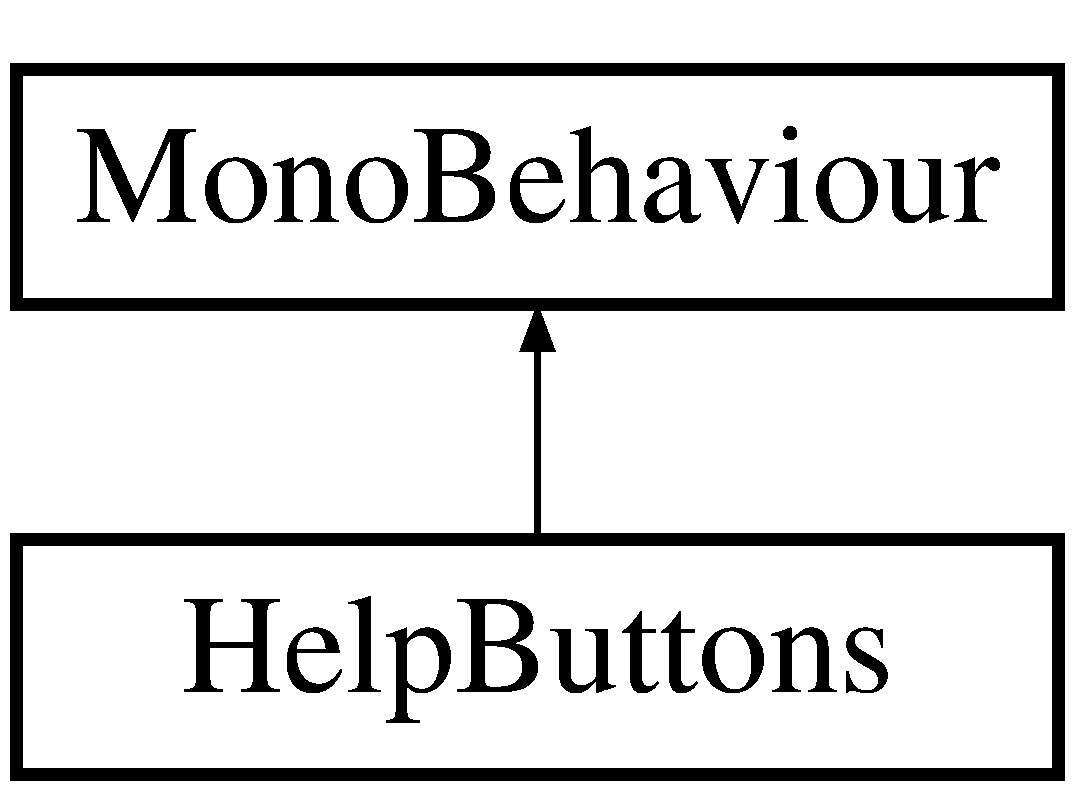
\includegraphics[height=2.000000cm]{class_help_buttons}
\end{center}
\end{figure}
\subsection*{Public Member Functions}
\begin{DoxyCompactItemize}
\item 
void \hyperlink{class_help_buttons_a9726fde5562db44998eb42b897de48ac}{show\+Help\+Text} ()
\end{DoxyCompactItemize}
\subsection*{Public Attributes}
\begin{DoxyCompactItemize}
\item 
Text \hyperlink{class_help_buttons_ab183c5e89514936aac4fdb0fb27d3ba3}{help\+Text}
\item 
\hyperlink{class_analytics_by_level}{Analytics\+By\+Level} \hyperlink{class_help_buttons_ad47263338c2ea5515badf5dc8a8bb18b}{level\+Analytics}
\end{DoxyCompactItemize}


\subsection{Member Function Documentation}
\mbox{\Hypertarget{class_help_buttons_a9726fde5562db44998eb42b897de48ac}\label{class_help_buttons_a9726fde5562db44998eb42b897de48ac}} 
\index{Help\+Buttons@{Help\+Buttons}!show\+Help\+Text@{show\+Help\+Text}}
\index{show\+Help\+Text@{show\+Help\+Text}!Help\+Buttons@{Help\+Buttons}}
\subsubsection{\texorpdfstring{show\+Help\+Text()}{showHelpText()}}
{\footnotesize\ttfamily void Help\+Buttons.\+show\+Help\+Text (\begin{DoxyParamCaption}{ }\end{DoxyParamCaption})}



\subsection{Member Data Documentation}
\mbox{\Hypertarget{class_help_buttons_ab183c5e89514936aac4fdb0fb27d3ba3}\label{class_help_buttons_ab183c5e89514936aac4fdb0fb27d3ba3}} 
\index{Help\+Buttons@{Help\+Buttons}!help\+Text@{help\+Text}}
\index{help\+Text@{help\+Text}!Help\+Buttons@{Help\+Buttons}}
\subsubsection{\texorpdfstring{help\+Text}{helpText}}
{\footnotesize\ttfamily Text Help\+Buttons.\+help\+Text}

\mbox{\Hypertarget{class_help_buttons_ad47263338c2ea5515badf5dc8a8bb18b}\label{class_help_buttons_ad47263338c2ea5515badf5dc8a8bb18b}} 
\index{Help\+Buttons@{Help\+Buttons}!level\+Analytics@{level\+Analytics}}
\index{level\+Analytics@{level\+Analytics}!Help\+Buttons@{Help\+Buttons}}
\subsubsection{\texorpdfstring{level\+Analytics}{levelAnalytics}}
{\footnotesize\ttfamily \hyperlink{class_analytics_by_level}{Analytics\+By\+Level} Help\+Buttons.\+level\+Analytics}



The documentation for this class was generated from the following file\+:\begin{DoxyCompactItemize}
\item 
/\+Users/kwanholloway/git/5001\+Project/\+Game\+Project/\+Assets/\+Scripts/\+Game\+Logic/\hyperlink{_help_buttons_8cs}{Help\+Buttons.\+cs}\end{DoxyCompactItemize}

\hypertarget{class_indent_puzzle}{}\section{Indent\+Puzzle Class Reference}
\label{class_indent_puzzle}\index{Indent\+Puzzle@{Indent\+Puzzle}}
Inheritance diagram for Indent\+Puzzle\+:\begin{figure}[H]
\begin{center}
\leavevmode
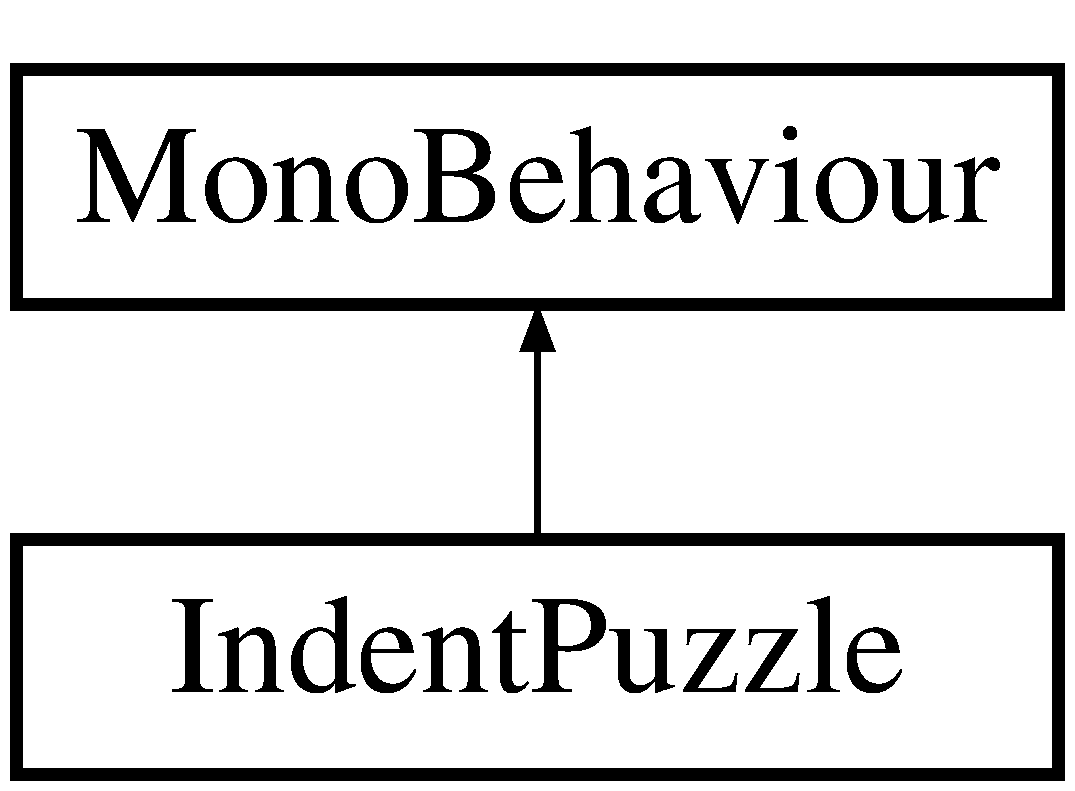
\includegraphics[height=2.000000cm]{class_indent_puzzle}
\end{center}
\end{figure}
\subsection*{Public Member Functions}
\begin{DoxyCompactItemize}
\item 
void \hyperlink{class_indent_puzzle_a215e6d882d3f871e695a6ee0d21378a2}{indent\+Button\+One} ()
\item 
void \hyperlink{class_indent_puzzle_ab75ac1bbe900470f0eb4ab3040bb18e5}{unindent\+Button\+One} ()
\item 
void \hyperlink{class_indent_puzzle_a4f628be71f4f814df6684303d10fb121}{indent\+Button\+Two} ()
\item 
void \hyperlink{class_indent_puzzle_a3c861e4dffc0b8c5241b8f64d073679b}{unindent\+Button\+Two} ()
\item 
void \hyperlink{class_indent_puzzle_a1d0b6f844214804ae157af4be1fb780d}{indent\+Button\+Three} ()
\item 
void \hyperlink{class_indent_puzzle_a66535f1875dc7b668f1c54e122914e33}{unindent\+Button\+Three} ()
\item 
void \hyperlink{class_indent_puzzle_af180ebdc9af7a5550a7d2099c4c05eea}{indent\+Button\+Four} ()
\item 
void \hyperlink{class_indent_puzzle_a3a68645b408c0649e237fa77c79ffa15}{unindent\+Button\+Four} ()
\item 
void \hyperlink{class_indent_puzzle_a6d494b8306dfbdc444d67032f6dbb275}{indent\+Button\+Five} ()
\item 
void \hyperlink{class_indent_puzzle_a4aabfa2cd19fadbb5d2e13d4e6defa1d}{unindent\+Button\+Five} ()
\item 
void \hyperlink{class_indent_puzzle_a415f779d82c83fb96cde45421a684f43}{reset\+Lines} ()
\end{DoxyCompactItemize}
\subsection*{Public Attributes}
\begin{DoxyCompactItemize}
\item 
Game\+Object \hyperlink{class_indent_puzzle_a4e40070466818e4679b394d5bda86ade}{text\+Line\+One}
\item 
Game\+Object \hyperlink{class_indent_puzzle_ad9cebfab9a44877b5bbed7549fcc08fd}{text\+Line\+Two}
\item 
Game\+Object \hyperlink{class_indent_puzzle_a9089446322d12f009d2f8b97a4c0fecd}{text\+Line\+Three}
\item 
Game\+Object \hyperlink{class_indent_puzzle_a1f2af93e171a1a996f1332be17f5fb49}{text\+Line\+Four}
\item 
Game\+Object \hyperlink{class_indent_puzzle_ac10f8edc26d7c44680c010d0131bae4f}{text\+Line\+Five}
\item 
int \hyperlink{class_indent_puzzle_ad84195fdc4df72f77f9638857240d067}{indent\+Counter\+One} = 0
\item 
int \hyperlink{class_indent_puzzle_a61233af419d8df3e8720411babf513d3}{indent\+Counter\+Two} = 0
\item 
int \hyperlink{class_indent_puzzle_a59902da46bba63163638c8eb871f1e0f}{indent\+Counter\+Three} = 0
\item 
int \hyperlink{class_indent_puzzle_a660de35fb6850ef5c6f88fd93dac427a}{indent\+Counter\+Four} = 0
\item 
int \hyperlink{class_indent_puzzle_abd24d4138f4bb377624e1d1da061857d}{indent\+Counter\+Five} = 0
\end{DoxyCompactItemize}


\subsection{Member Function Documentation}
\mbox{\Hypertarget{class_indent_puzzle_a6d494b8306dfbdc444d67032f6dbb275}\label{class_indent_puzzle_a6d494b8306dfbdc444d67032f6dbb275}} 
\index{Indent\+Puzzle@{Indent\+Puzzle}!indent\+Button\+Five@{indent\+Button\+Five}}
\index{indent\+Button\+Five@{indent\+Button\+Five}!Indent\+Puzzle@{Indent\+Puzzle}}
\subsubsection{\texorpdfstring{indent\+Button\+Five()}{indentButtonFive()}}
{\footnotesize\ttfamily void Indent\+Puzzle.\+indent\+Button\+Five (\begin{DoxyParamCaption}{ }\end{DoxyParamCaption})}

\mbox{\Hypertarget{class_indent_puzzle_af180ebdc9af7a5550a7d2099c4c05eea}\label{class_indent_puzzle_af180ebdc9af7a5550a7d2099c4c05eea}} 
\index{Indent\+Puzzle@{Indent\+Puzzle}!indent\+Button\+Four@{indent\+Button\+Four}}
\index{indent\+Button\+Four@{indent\+Button\+Four}!Indent\+Puzzle@{Indent\+Puzzle}}
\subsubsection{\texorpdfstring{indent\+Button\+Four()}{indentButtonFour()}}
{\footnotesize\ttfamily void Indent\+Puzzle.\+indent\+Button\+Four (\begin{DoxyParamCaption}{ }\end{DoxyParamCaption})}

\mbox{\Hypertarget{class_indent_puzzle_a215e6d882d3f871e695a6ee0d21378a2}\label{class_indent_puzzle_a215e6d882d3f871e695a6ee0d21378a2}} 
\index{Indent\+Puzzle@{Indent\+Puzzle}!indent\+Button\+One@{indent\+Button\+One}}
\index{indent\+Button\+One@{indent\+Button\+One}!Indent\+Puzzle@{Indent\+Puzzle}}
\subsubsection{\texorpdfstring{indent\+Button\+One()}{indentButtonOne()}}
{\footnotesize\ttfamily void Indent\+Puzzle.\+indent\+Button\+One (\begin{DoxyParamCaption}{ }\end{DoxyParamCaption})}

\mbox{\Hypertarget{class_indent_puzzle_a1d0b6f844214804ae157af4be1fb780d}\label{class_indent_puzzle_a1d0b6f844214804ae157af4be1fb780d}} 
\index{Indent\+Puzzle@{Indent\+Puzzle}!indent\+Button\+Three@{indent\+Button\+Three}}
\index{indent\+Button\+Three@{indent\+Button\+Three}!Indent\+Puzzle@{Indent\+Puzzle}}
\subsubsection{\texorpdfstring{indent\+Button\+Three()}{indentButtonThree()}}
{\footnotesize\ttfamily void Indent\+Puzzle.\+indent\+Button\+Three (\begin{DoxyParamCaption}{ }\end{DoxyParamCaption})}

\mbox{\Hypertarget{class_indent_puzzle_a4f628be71f4f814df6684303d10fb121}\label{class_indent_puzzle_a4f628be71f4f814df6684303d10fb121}} 
\index{Indent\+Puzzle@{Indent\+Puzzle}!indent\+Button\+Two@{indent\+Button\+Two}}
\index{indent\+Button\+Two@{indent\+Button\+Two}!Indent\+Puzzle@{Indent\+Puzzle}}
\subsubsection{\texorpdfstring{indent\+Button\+Two()}{indentButtonTwo()}}
{\footnotesize\ttfamily void Indent\+Puzzle.\+indent\+Button\+Two (\begin{DoxyParamCaption}{ }\end{DoxyParamCaption})}

\mbox{\Hypertarget{class_indent_puzzle_a415f779d82c83fb96cde45421a684f43}\label{class_indent_puzzle_a415f779d82c83fb96cde45421a684f43}} 
\index{Indent\+Puzzle@{Indent\+Puzzle}!reset\+Lines@{reset\+Lines}}
\index{reset\+Lines@{reset\+Lines}!Indent\+Puzzle@{Indent\+Puzzle}}
\subsubsection{\texorpdfstring{reset\+Lines()}{resetLines()}}
{\footnotesize\ttfamily void Indent\+Puzzle.\+reset\+Lines (\begin{DoxyParamCaption}{ }\end{DoxyParamCaption})}

\mbox{\Hypertarget{class_indent_puzzle_a4aabfa2cd19fadbb5d2e13d4e6defa1d}\label{class_indent_puzzle_a4aabfa2cd19fadbb5d2e13d4e6defa1d}} 
\index{Indent\+Puzzle@{Indent\+Puzzle}!unindent\+Button\+Five@{unindent\+Button\+Five}}
\index{unindent\+Button\+Five@{unindent\+Button\+Five}!Indent\+Puzzle@{Indent\+Puzzle}}
\subsubsection{\texorpdfstring{unindent\+Button\+Five()}{unindentButtonFive()}}
{\footnotesize\ttfamily void Indent\+Puzzle.\+unindent\+Button\+Five (\begin{DoxyParamCaption}{ }\end{DoxyParamCaption})}

\mbox{\Hypertarget{class_indent_puzzle_a3a68645b408c0649e237fa77c79ffa15}\label{class_indent_puzzle_a3a68645b408c0649e237fa77c79ffa15}} 
\index{Indent\+Puzzle@{Indent\+Puzzle}!unindent\+Button\+Four@{unindent\+Button\+Four}}
\index{unindent\+Button\+Four@{unindent\+Button\+Four}!Indent\+Puzzle@{Indent\+Puzzle}}
\subsubsection{\texorpdfstring{unindent\+Button\+Four()}{unindentButtonFour()}}
{\footnotesize\ttfamily void Indent\+Puzzle.\+unindent\+Button\+Four (\begin{DoxyParamCaption}{ }\end{DoxyParamCaption})}

\mbox{\Hypertarget{class_indent_puzzle_ab75ac1bbe900470f0eb4ab3040bb18e5}\label{class_indent_puzzle_ab75ac1bbe900470f0eb4ab3040bb18e5}} 
\index{Indent\+Puzzle@{Indent\+Puzzle}!unindent\+Button\+One@{unindent\+Button\+One}}
\index{unindent\+Button\+One@{unindent\+Button\+One}!Indent\+Puzzle@{Indent\+Puzzle}}
\subsubsection{\texorpdfstring{unindent\+Button\+One()}{unindentButtonOne()}}
{\footnotesize\ttfamily void Indent\+Puzzle.\+unindent\+Button\+One (\begin{DoxyParamCaption}{ }\end{DoxyParamCaption})}

\mbox{\Hypertarget{class_indent_puzzle_a66535f1875dc7b668f1c54e122914e33}\label{class_indent_puzzle_a66535f1875dc7b668f1c54e122914e33}} 
\index{Indent\+Puzzle@{Indent\+Puzzle}!unindent\+Button\+Three@{unindent\+Button\+Three}}
\index{unindent\+Button\+Three@{unindent\+Button\+Three}!Indent\+Puzzle@{Indent\+Puzzle}}
\subsubsection{\texorpdfstring{unindent\+Button\+Three()}{unindentButtonThree()}}
{\footnotesize\ttfamily void Indent\+Puzzle.\+unindent\+Button\+Three (\begin{DoxyParamCaption}{ }\end{DoxyParamCaption})}

\mbox{\Hypertarget{class_indent_puzzle_a3c861e4dffc0b8c5241b8f64d073679b}\label{class_indent_puzzle_a3c861e4dffc0b8c5241b8f64d073679b}} 
\index{Indent\+Puzzle@{Indent\+Puzzle}!unindent\+Button\+Two@{unindent\+Button\+Two}}
\index{unindent\+Button\+Two@{unindent\+Button\+Two}!Indent\+Puzzle@{Indent\+Puzzle}}
\subsubsection{\texorpdfstring{unindent\+Button\+Two()}{unindentButtonTwo()}}
{\footnotesize\ttfamily void Indent\+Puzzle.\+unindent\+Button\+Two (\begin{DoxyParamCaption}{ }\end{DoxyParamCaption})}



\subsection{Member Data Documentation}
\mbox{\Hypertarget{class_indent_puzzle_abd24d4138f4bb377624e1d1da061857d}\label{class_indent_puzzle_abd24d4138f4bb377624e1d1da061857d}} 
\index{Indent\+Puzzle@{Indent\+Puzzle}!indent\+Counter\+Five@{indent\+Counter\+Five}}
\index{indent\+Counter\+Five@{indent\+Counter\+Five}!Indent\+Puzzle@{Indent\+Puzzle}}
\subsubsection{\texorpdfstring{indent\+Counter\+Five}{indentCounterFive}}
{\footnotesize\ttfamily int Indent\+Puzzle.\+indent\+Counter\+Five = 0}

\mbox{\Hypertarget{class_indent_puzzle_a660de35fb6850ef5c6f88fd93dac427a}\label{class_indent_puzzle_a660de35fb6850ef5c6f88fd93dac427a}} 
\index{Indent\+Puzzle@{Indent\+Puzzle}!indent\+Counter\+Four@{indent\+Counter\+Four}}
\index{indent\+Counter\+Four@{indent\+Counter\+Four}!Indent\+Puzzle@{Indent\+Puzzle}}
\subsubsection{\texorpdfstring{indent\+Counter\+Four}{indentCounterFour}}
{\footnotesize\ttfamily int Indent\+Puzzle.\+indent\+Counter\+Four = 0}

\mbox{\Hypertarget{class_indent_puzzle_ad84195fdc4df72f77f9638857240d067}\label{class_indent_puzzle_ad84195fdc4df72f77f9638857240d067}} 
\index{Indent\+Puzzle@{Indent\+Puzzle}!indent\+Counter\+One@{indent\+Counter\+One}}
\index{indent\+Counter\+One@{indent\+Counter\+One}!Indent\+Puzzle@{Indent\+Puzzle}}
\subsubsection{\texorpdfstring{indent\+Counter\+One}{indentCounterOne}}
{\footnotesize\ttfamily int Indent\+Puzzle.\+indent\+Counter\+One = 0}

\mbox{\Hypertarget{class_indent_puzzle_a59902da46bba63163638c8eb871f1e0f}\label{class_indent_puzzle_a59902da46bba63163638c8eb871f1e0f}} 
\index{Indent\+Puzzle@{Indent\+Puzzle}!indent\+Counter\+Three@{indent\+Counter\+Three}}
\index{indent\+Counter\+Three@{indent\+Counter\+Three}!Indent\+Puzzle@{Indent\+Puzzle}}
\subsubsection{\texorpdfstring{indent\+Counter\+Three}{indentCounterThree}}
{\footnotesize\ttfamily int Indent\+Puzzle.\+indent\+Counter\+Three = 0}

\mbox{\Hypertarget{class_indent_puzzle_a61233af419d8df3e8720411babf513d3}\label{class_indent_puzzle_a61233af419d8df3e8720411babf513d3}} 
\index{Indent\+Puzzle@{Indent\+Puzzle}!indent\+Counter\+Two@{indent\+Counter\+Two}}
\index{indent\+Counter\+Two@{indent\+Counter\+Two}!Indent\+Puzzle@{Indent\+Puzzle}}
\subsubsection{\texorpdfstring{indent\+Counter\+Two}{indentCounterTwo}}
{\footnotesize\ttfamily int Indent\+Puzzle.\+indent\+Counter\+Two = 0}

\mbox{\Hypertarget{class_indent_puzzle_ac10f8edc26d7c44680c010d0131bae4f}\label{class_indent_puzzle_ac10f8edc26d7c44680c010d0131bae4f}} 
\index{Indent\+Puzzle@{Indent\+Puzzle}!text\+Line\+Five@{text\+Line\+Five}}
\index{text\+Line\+Five@{text\+Line\+Five}!Indent\+Puzzle@{Indent\+Puzzle}}
\subsubsection{\texorpdfstring{text\+Line\+Five}{textLineFive}}
{\footnotesize\ttfamily Game\+Object Indent\+Puzzle.\+text\+Line\+Five}

\mbox{\Hypertarget{class_indent_puzzle_a1f2af93e171a1a996f1332be17f5fb49}\label{class_indent_puzzle_a1f2af93e171a1a996f1332be17f5fb49}} 
\index{Indent\+Puzzle@{Indent\+Puzzle}!text\+Line\+Four@{text\+Line\+Four}}
\index{text\+Line\+Four@{text\+Line\+Four}!Indent\+Puzzle@{Indent\+Puzzle}}
\subsubsection{\texorpdfstring{text\+Line\+Four}{textLineFour}}
{\footnotesize\ttfamily Game\+Object Indent\+Puzzle.\+text\+Line\+Four}

\mbox{\Hypertarget{class_indent_puzzle_a4e40070466818e4679b394d5bda86ade}\label{class_indent_puzzle_a4e40070466818e4679b394d5bda86ade}} 
\index{Indent\+Puzzle@{Indent\+Puzzle}!text\+Line\+One@{text\+Line\+One}}
\index{text\+Line\+One@{text\+Line\+One}!Indent\+Puzzle@{Indent\+Puzzle}}
\subsubsection{\texorpdfstring{text\+Line\+One}{textLineOne}}
{\footnotesize\ttfamily Game\+Object Indent\+Puzzle.\+text\+Line\+One}

\mbox{\Hypertarget{class_indent_puzzle_a9089446322d12f009d2f8b97a4c0fecd}\label{class_indent_puzzle_a9089446322d12f009d2f8b97a4c0fecd}} 
\index{Indent\+Puzzle@{Indent\+Puzzle}!text\+Line\+Three@{text\+Line\+Three}}
\index{text\+Line\+Three@{text\+Line\+Three}!Indent\+Puzzle@{Indent\+Puzzle}}
\subsubsection{\texorpdfstring{text\+Line\+Three}{textLineThree}}
{\footnotesize\ttfamily Game\+Object Indent\+Puzzle.\+text\+Line\+Three}

\mbox{\Hypertarget{class_indent_puzzle_ad9cebfab9a44877b5bbed7549fcc08fd}\label{class_indent_puzzle_ad9cebfab9a44877b5bbed7549fcc08fd}} 
\index{Indent\+Puzzle@{Indent\+Puzzle}!text\+Line\+Two@{text\+Line\+Two}}
\index{text\+Line\+Two@{text\+Line\+Two}!Indent\+Puzzle@{Indent\+Puzzle}}
\subsubsection{\texorpdfstring{text\+Line\+Two}{textLineTwo}}
{\footnotesize\ttfamily Game\+Object Indent\+Puzzle.\+text\+Line\+Two}



The documentation for this class was generated from the following file\+:\begin{DoxyCompactItemize}
\item 
/\+Users/kwanholloway/git/5001\+Project/\+Game\+Project/\+Assets/\+Scripts/\+Game\+Logic/\hyperlink{_indent_puzzle_8cs}{Indent\+Puzzle.\+cs}\end{DoxyCompactItemize}

\hypertarget{class_insert_puzzle_completion}{}\section{Insert\+Puzzle\+Completion Class Reference}
\label{class_insert_puzzle_completion}\index{Insert\+Puzzle\+Completion@{Insert\+Puzzle\+Completion}}
Inheritance diagram for Insert\+Puzzle\+Completion\+:\begin{figure}[H]
\begin{center}
\leavevmode
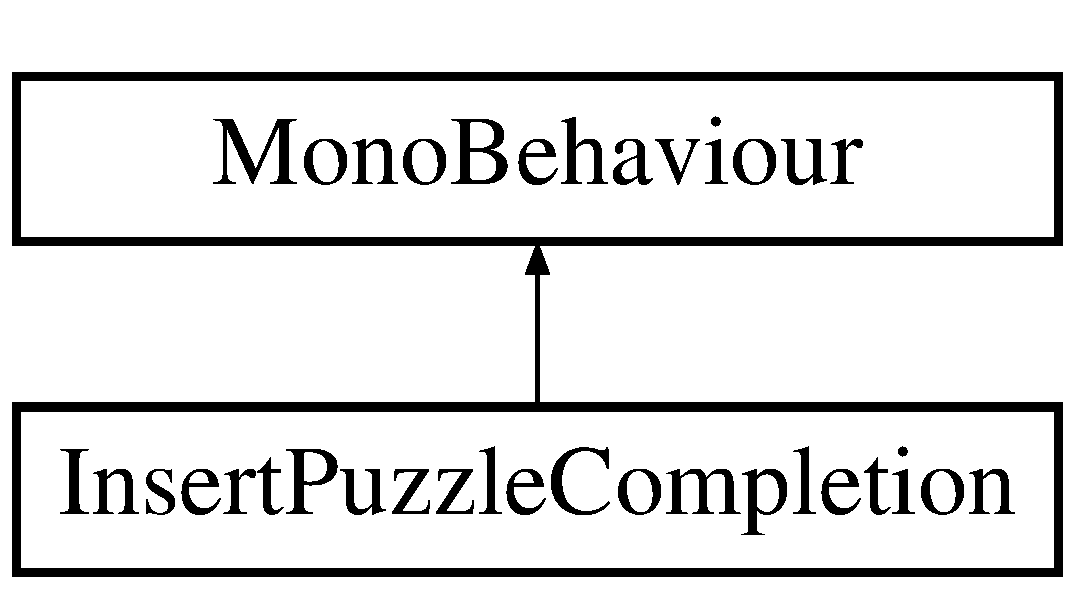
\includegraphics[height=2.000000cm]{class_insert_puzzle_completion}
\end{center}
\end{figure}
\subsection*{Public Member Functions}
\begin{DoxyCompactItemize}
\item 
void \hyperlink{class_insert_puzzle_completion_a63718180926a577838dc477e4c9eeb1d}{open\+Door} ()
\item 
void \hyperlink{class_insert_puzzle_completion_a440c8d4d6b16f8c21edc989c9adbac4a}{close\+Door} ()
\end{DoxyCompactItemize}
\subsection*{Public Attributes}
\begin{DoxyCompactItemize}
\item 
\hyperlink{class_indent_puzzle}{Indent\+Puzzle} \hyperlink{class_insert_puzzle_completion_a578d448dd1fae88d97493a0f46b3ddd0}{line\+One}
\item 
\hyperlink{class_indent_puzzle}{Indent\+Puzzle} \hyperlink{class_insert_puzzle_completion_a90e3355e28d38eed7b71ab656607af65}{line\+Two}
\item 
\hyperlink{class_indent_puzzle}{Indent\+Puzzle} \hyperlink{class_insert_puzzle_completion_a52a264da1931ee1d58db091081843024}{line\+Three}
\item 
\hyperlink{class_indent_puzzle}{Indent\+Puzzle} \hyperlink{class_insert_puzzle_completion_a4dfdeae27ea5824db458883961b9d1e5}{line\+Four}
\item 
\hyperlink{class_indent_puzzle}{Indent\+Puzzle} \hyperlink{class_insert_puzzle_completion_a3069beb9bba0c0cfbcd52bd5e49db135}{line\+Five}
\item 
Game\+Object \hyperlink{class_insert_puzzle_completion_ad2291f7238e8f7ee355583d0a9da8b49}{door\+One}
\item 
bool \hyperlink{class_insert_puzzle_completion_a6184f335f81f3b544e6b065a9cccc084}{puzzle\+Finished}
\end{DoxyCompactItemize}


\subsection{Member Function Documentation}
\mbox{\Hypertarget{class_insert_puzzle_completion_a440c8d4d6b16f8c21edc989c9adbac4a}\label{class_insert_puzzle_completion_a440c8d4d6b16f8c21edc989c9adbac4a}} 
\index{Insert\+Puzzle\+Completion@{Insert\+Puzzle\+Completion}!close\+Door@{close\+Door}}
\index{close\+Door@{close\+Door}!Insert\+Puzzle\+Completion@{Insert\+Puzzle\+Completion}}
\subsubsection{\texorpdfstring{close\+Door()}{closeDoor()}}
{\footnotesize\ttfamily void Insert\+Puzzle\+Completion.\+close\+Door (\begin{DoxyParamCaption}{ }\end{DoxyParamCaption})}

\mbox{\Hypertarget{class_insert_puzzle_completion_a63718180926a577838dc477e4c9eeb1d}\label{class_insert_puzzle_completion_a63718180926a577838dc477e4c9eeb1d}} 
\index{Insert\+Puzzle\+Completion@{Insert\+Puzzle\+Completion}!open\+Door@{open\+Door}}
\index{open\+Door@{open\+Door}!Insert\+Puzzle\+Completion@{Insert\+Puzzle\+Completion}}
\subsubsection{\texorpdfstring{open\+Door()}{openDoor()}}
{\footnotesize\ttfamily void Insert\+Puzzle\+Completion.\+open\+Door (\begin{DoxyParamCaption}{ }\end{DoxyParamCaption})}



\subsection{Member Data Documentation}
\mbox{\Hypertarget{class_insert_puzzle_completion_ad2291f7238e8f7ee355583d0a9da8b49}\label{class_insert_puzzle_completion_ad2291f7238e8f7ee355583d0a9da8b49}} 
\index{Insert\+Puzzle\+Completion@{Insert\+Puzzle\+Completion}!door\+One@{door\+One}}
\index{door\+One@{door\+One}!Insert\+Puzzle\+Completion@{Insert\+Puzzle\+Completion}}
\subsubsection{\texorpdfstring{door\+One}{doorOne}}
{\footnotesize\ttfamily Game\+Object Insert\+Puzzle\+Completion.\+door\+One}

\mbox{\Hypertarget{class_insert_puzzle_completion_a3069beb9bba0c0cfbcd52bd5e49db135}\label{class_insert_puzzle_completion_a3069beb9bba0c0cfbcd52bd5e49db135}} 
\index{Insert\+Puzzle\+Completion@{Insert\+Puzzle\+Completion}!line\+Five@{line\+Five}}
\index{line\+Five@{line\+Five}!Insert\+Puzzle\+Completion@{Insert\+Puzzle\+Completion}}
\subsubsection{\texorpdfstring{line\+Five}{lineFive}}
{\footnotesize\ttfamily \hyperlink{class_indent_puzzle}{Indent\+Puzzle} Insert\+Puzzle\+Completion.\+line\+Five}

\mbox{\Hypertarget{class_insert_puzzle_completion_a4dfdeae27ea5824db458883961b9d1e5}\label{class_insert_puzzle_completion_a4dfdeae27ea5824db458883961b9d1e5}} 
\index{Insert\+Puzzle\+Completion@{Insert\+Puzzle\+Completion}!line\+Four@{line\+Four}}
\index{line\+Four@{line\+Four}!Insert\+Puzzle\+Completion@{Insert\+Puzzle\+Completion}}
\subsubsection{\texorpdfstring{line\+Four}{lineFour}}
{\footnotesize\ttfamily \hyperlink{class_indent_puzzle}{Indent\+Puzzle} Insert\+Puzzle\+Completion.\+line\+Four}

\mbox{\Hypertarget{class_insert_puzzle_completion_a578d448dd1fae88d97493a0f46b3ddd0}\label{class_insert_puzzle_completion_a578d448dd1fae88d97493a0f46b3ddd0}} 
\index{Insert\+Puzzle\+Completion@{Insert\+Puzzle\+Completion}!line\+One@{line\+One}}
\index{line\+One@{line\+One}!Insert\+Puzzle\+Completion@{Insert\+Puzzle\+Completion}}
\subsubsection{\texorpdfstring{line\+One}{lineOne}}
{\footnotesize\ttfamily \hyperlink{class_indent_puzzle}{Indent\+Puzzle} Insert\+Puzzle\+Completion.\+line\+One}

\mbox{\Hypertarget{class_insert_puzzle_completion_a52a264da1931ee1d58db091081843024}\label{class_insert_puzzle_completion_a52a264da1931ee1d58db091081843024}} 
\index{Insert\+Puzzle\+Completion@{Insert\+Puzzle\+Completion}!line\+Three@{line\+Three}}
\index{line\+Three@{line\+Three}!Insert\+Puzzle\+Completion@{Insert\+Puzzle\+Completion}}
\subsubsection{\texorpdfstring{line\+Three}{lineThree}}
{\footnotesize\ttfamily \hyperlink{class_indent_puzzle}{Indent\+Puzzle} Insert\+Puzzle\+Completion.\+line\+Three}

\mbox{\Hypertarget{class_insert_puzzle_completion_a90e3355e28d38eed7b71ab656607af65}\label{class_insert_puzzle_completion_a90e3355e28d38eed7b71ab656607af65}} 
\index{Insert\+Puzzle\+Completion@{Insert\+Puzzle\+Completion}!line\+Two@{line\+Two}}
\index{line\+Two@{line\+Two}!Insert\+Puzzle\+Completion@{Insert\+Puzzle\+Completion}}
\subsubsection{\texorpdfstring{line\+Two}{lineTwo}}
{\footnotesize\ttfamily \hyperlink{class_indent_puzzle}{Indent\+Puzzle} Insert\+Puzzle\+Completion.\+line\+Two}

\mbox{\Hypertarget{class_insert_puzzle_completion_a6184f335f81f3b544e6b065a9cccc084}\label{class_insert_puzzle_completion_a6184f335f81f3b544e6b065a9cccc084}} 
\index{Insert\+Puzzle\+Completion@{Insert\+Puzzle\+Completion}!puzzle\+Finished@{puzzle\+Finished}}
\index{puzzle\+Finished@{puzzle\+Finished}!Insert\+Puzzle\+Completion@{Insert\+Puzzle\+Completion}}
\subsubsection{\texorpdfstring{puzzle\+Finished}{puzzleFinished}}
{\footnotesize\ttfamily bool Insert\+Puzzle\+Completion.\+puzzle\+Finished}



The documentation for this class was generated from the following file\+:\begin{DoxyCompactItemize}
\item 
/\+Users/kwanholloway/git/5001\+Project/\+Game\+Project/\+Assets/\+Scripts/\+Puzzle\+Logic/\+Final\+Level/\hyperlink{_insert_puzzle_completion_8cs}{Insert\+Puzzle\+Completion.\+cs}\end{DoxyCompactItemize}

\hypertarget{class_intro_level_manager}{}\section{Intro\+Level\+Manager Class Reference}
\label{class_intro_level_manager}\index{Intro\+Level\+Manager@{Intro\+Level\+Manager}}
Inheritance diagram for Intro\+Level\+Manager\+:\begin{figure}[H]
\begin{center}
\leavevmode
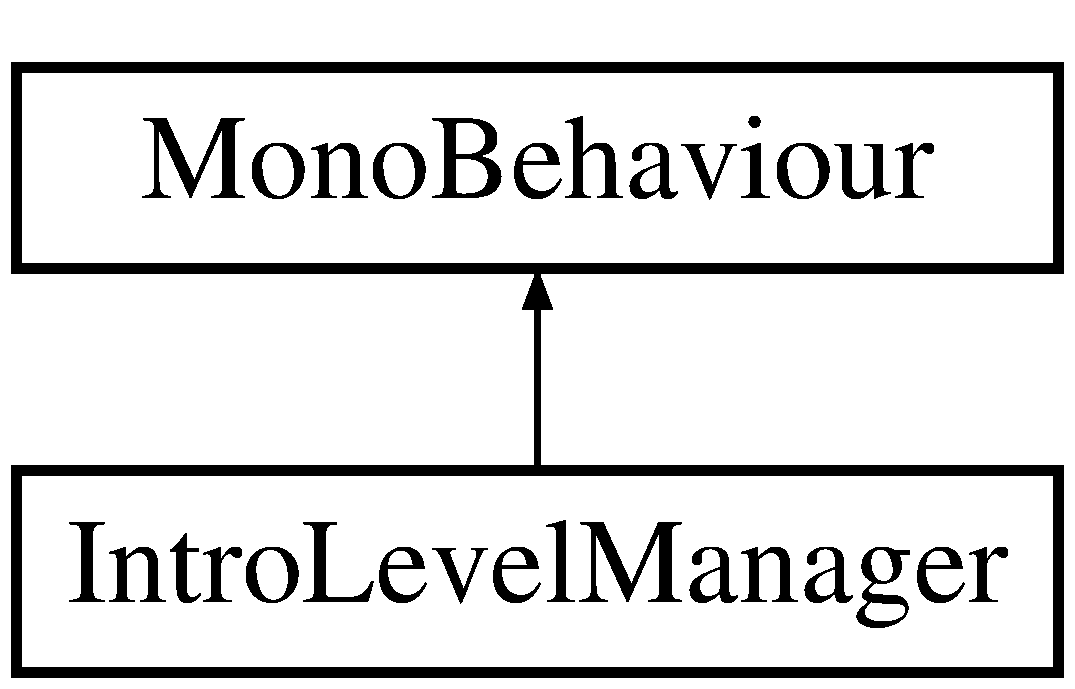
\includegraphics[height=2.000000cm]{class_intro_level_manager}
\end{center}
\end{figure}
\subsection*{Public Attributes}
\begin{DoxyCompactItemize}
\item 
Game\+Object \hyperlink{class_intro_level_manager_ad6a0e7ffa4f50654f032516f26d50058}{array\+Portal}
\item 
Game\+Object \hyperlink{class_intro_level_manager_aa84bfec3c06a01b9417f2f7a4eff5e39}{loop\+Portal}
\item 
float \hyperlink{class_intro_level_manager_a01ffda007d472014f877a8d70c66d3af}{x1} = 48.\+8f
\item 
float \hyperlink{class_intro_level_manager_ad1c4e0b7a9ef9ea24d72a21f20b86fc3}{x2} = 63.\+42f
\item 
float \hyperlink{class_intro_level_manager_a0e0549499a223271048ede469a256236}{y} = -\/2.\+7f
\end{DoxyCompactItemize}


\subsection{Member Data Documentation}
\mbox{\Hypertarget{class_intro_level_manager_ad6a0e7ffa4f50654f032516f26d50058}\label{class_intro_level_manager_ad6a0e7ffa4f50654f032516f26d50058}} 
\index{Intro\+Level\+Manager@{Intro\+Level\+Manager}!array\+Portal@{array\+Portal}}
\index{array\+Portal@{array\+Portal}!Intro\+Level\+Manager@{Intro\+Level\+Manager}}
\subsubsection{\texorpdfstring{array\+Portal}{arrayPortal}}
{\footnotesize\ttfamily Game\+Object Intro\+Level\+Manager.\+array\+Portal}

\mbox{\Hypertarget{class_intro_level_manager_aa84bfec3c06a01b9417f2f7a4eff5e39}\label{class_intro_level_manager_aa84bfec3c06a01b9417f2f7a4eff5e39}} 
\index{Intro\+Level\+Manager@{Intro\+Level\+Manager}!loop\+Portal@{loop\+Portal}}
\index{loop\+Portal@{loop\+Portal}!Intro\+Level\+Manager@{Intro\+Level\+Manager}}
\subsubsection{\texorpdfstring{loop\+Portal}{loopPortal}}
{\footnotesize\ttfamily Game\+Object Intro\+Level\+Manager.\+loop\+Portal}

\mbox{\Hypertarget{class_intro_level_manager_a01ffda007d472014f877a8d70c66d3af}\label{class_intro_level_manager_a01ffda007d472014f877a8d70c66d3af}} 
\index{Intro\+Level\+Manager@{Intro\+Level\+Manager}!x1@{x1}}
\index{x1@{x1}!Intro\+Level\+Manager@{Intro\+Level\+Manager}}
\subsubsection{\texorpdfstring{x1}{x1}}
{\footnotesize\ttfamily float Intro\+Level\+Manager.\+x1 = 48.\+8f}

\mbox{\Hypertarget{class_intro_level_manager_ad1c4e0b7a9ef9ea24d72a21f20b86fc3}\label{class_intro_level_manager_ad1c4e0b7a9ef9ea24d72a21f20b86fc3}} 
\index{Intro\+Level\+Manager@{Intro\+Level\+Manager}!x2@{x2}}
\index{x2@{x2}!Intro\+Level\+Manager@{Intro\+Level\+Manager}}
\subsubsection{\texorpdfstring{x2}{x2}}
{\footnotesize\ttfamily float Intro\+Level\+Manager.\+x2 = 63.\+42f}

\mbox{\Hypertarget{class_intro_level_manager_a0e0549499a223271048ede469a256236}\label{class_intro_level_manager_a0e0549499a223271048ede469a256236}} 
\index{Intro\+Level\+Manager@{Intro\+Level\+Manager}!y@{y}}
\index{y@{y}!Intro\+Level\+Manager@{Intro\+Level\+Manager}}
\subsubsection{\texorpdfstring{y}{y}}
{\footnotesize\ttfamily float Intro\+Level\+Manager.\+y = -\/2.\+7f}



The documentation for this class was generated from the following file\+:\begin{DoxyCompactItemize}
\item 
/\+Users/kwanholloway/git/5001\+Project/\+Game\+Project/\+Assets/\+Scripts/\+Game\+Logic/\hyperlink{_intro_level_manager_8cs}{Intro\+Level\+Manager.\+cs}\end{DoxyCompactItemize}

\hypertarget{class_j_i_t_level1}{}\section{J\+I\+T\+Level1 Class Reference}
\label{class_j_i_t_level1}\index{J\+I\+T\+Level1@{J\+I\+T\+Level1}}
Inheritance diagram for J\+I\+T\+Level1\+:\begin{figure}[H]
\begin{center}
\leavevmode
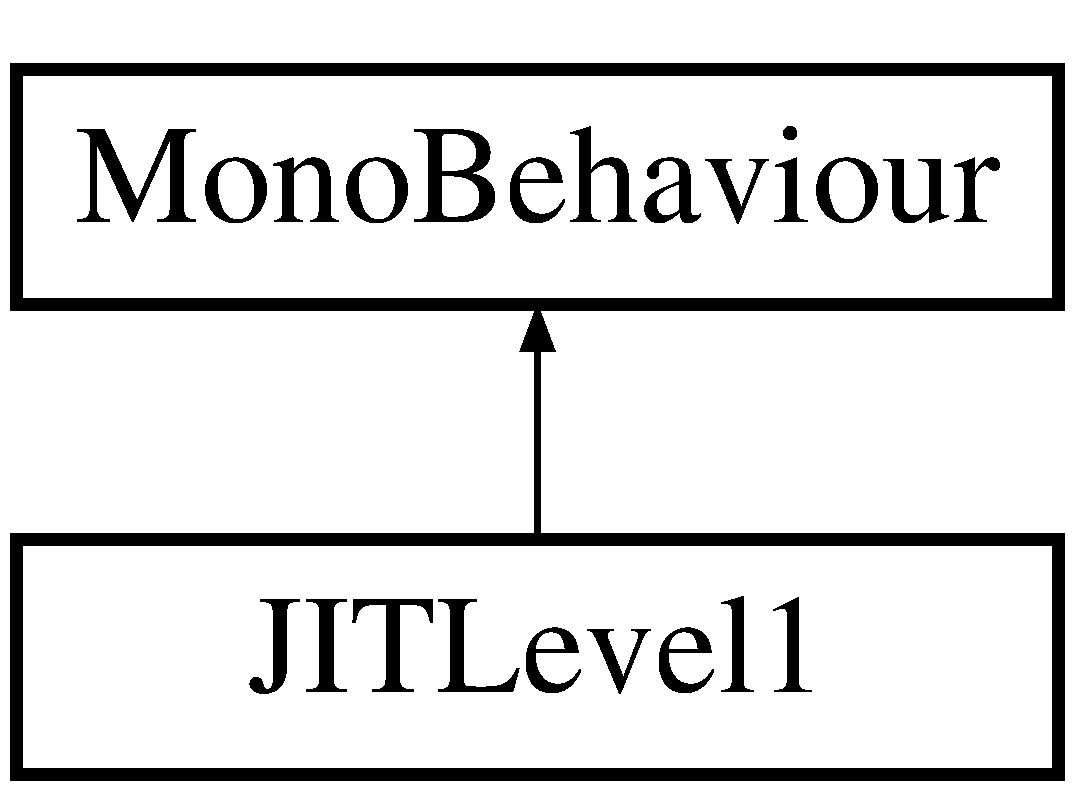
\includegraphics[height=2.000000cm]{class_j_i_t_level1}
\end{center}
\end{figure}
\subsection*{Public Attributes}
\begin{DoxyCompactItemize}
\item 
Game\+Object \hyperlink{class_j_i_t_level1_a39d30f1b60aeda6da0939f83a45c6a72}{jit}
\end{DoxyCompactItemize}


\subsection{Member Data Documentation}
\mbox{\Hypertarget{class_j_i_t_level1_a39d30f1b60aeda6da0939f83a45c6a72}\label{class_j_i_t_level1_a39d30f1b60aeda6da0939f83a45c6a72}} 
\index{J\+I\+T\+Level1@{J\+I\+T\+Level1}!jit@{jit}}
\index{jit@{jit}!J\+I\+T\+Level1@{J\+I\+T\+Level1}}
\subsubsection{\texorpdfstring{jit}{jit}}
{\footnotesize\ttfamily Game\+Object J\+I\+T\+Level1.\+jit}



The documentation for this class was generated from the following file\+:\begin{DoxyCompactItemize}
\item 
/\+Users/kwanholloway/git/5001\+Project/\+Game\+Project/\+Assets/\+Scripts/\+J\+I\+T\+Scripts/\hyperlink{_j_i_t_level1_8cs}{J\+I\+T\+Level1.\+cs}\end{DoxyCompactItemize}

\hypertarget{class_j_i_t_script}{}\section{J\+I\+T\+Script Class Reference}
\label{class_j_i_t_script}\index{J\+I\+T\+Script@{J\+I\+T\+Script}}
Inheritance diagram for J\+I\+T\+Script\+:\begin{figure}[H]
\begin{center}
\leavevmode
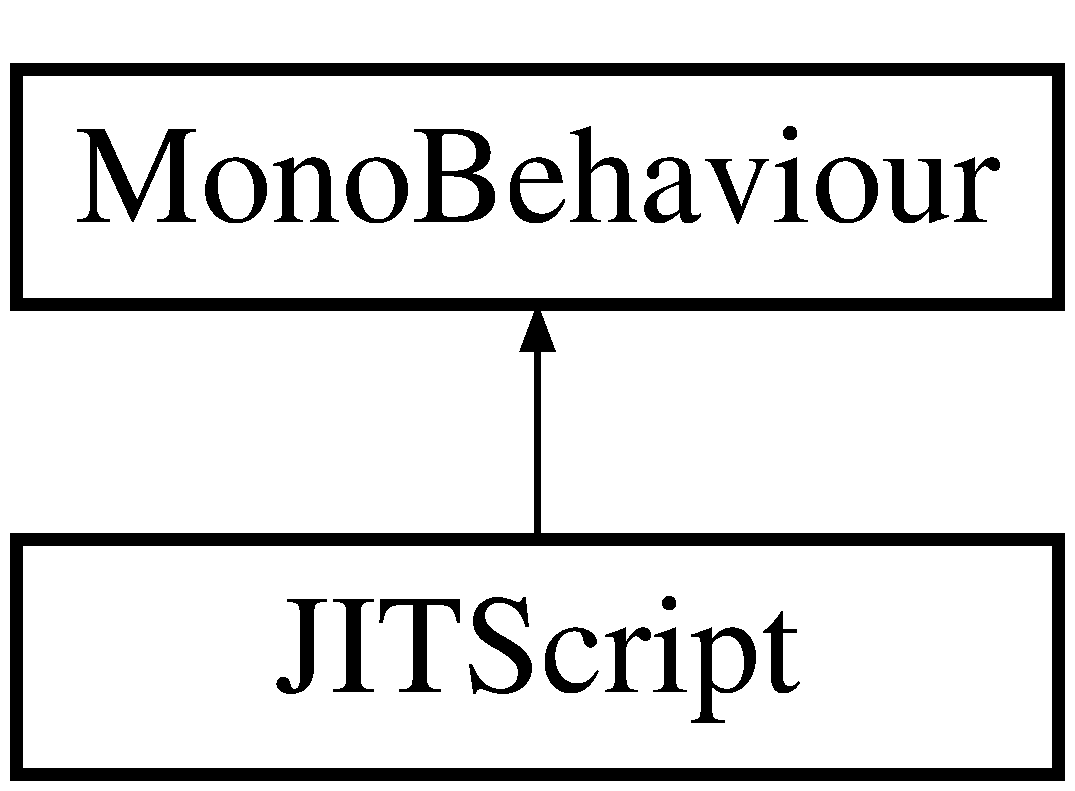
\includegraphics[height=2.000000cm]{class_j_i_t_script}
\end{center}
\end{figure}
\subsection*{Public Attributes}
\begin{DoxyCompactItemize}
\item 
Text \hyperlink{class_j_i_t_script_a033821b78a287d85204d336682fc6ee2}{word\+Display}
\item 
string \hyperlink{class_j_i_t_script_a47cba90f798093a7568d746789846520}{jit\+Name}
\item 
Audio\+Source \hyperlink{class_j_i_t_script_a3d065d627b861465a7c4da4c1ca9fdfd}{get\+Scientist\+Chime}
\end{DoxyCompactItemize}


\subsection{Detailed Description}
Handles all Just In Time Instructions and Promts in the game using an extensive switch statement 

\subsection{Member Data Documentation}
\mbox{\Hypertarget{class_j_i_t_script_a3d065d627b861465a7c4da4c1ca9fdfd}\label{class_j_i_t_script_a3d065d627b861465a7c4da4c1ca9fdfd}} 
\index{J\+I\+T\+Script@{J\+I\+T\+Script}!get\+Scientist\+Chime@{get\+Scientist\+Chime}}
\index{get\+Scientist\+Chime@{get\+Scientist\+Chime}!J\+I\+T\+Script@{J\+I\+T\+Script}}
\subsubsection{\texorpdfstring{get\+Scientist\+Chime}{getScientistChime}}
{\footnotesize\ttfamily Audio\+Source J\+I\+T\+Script.\+get\+Scientist\+Chime}

\mbox{\Hypertarget{class_j_i_t_script_a47cba90f798093a7568d746789846520}\label{class_j_i_t_script_a47cba90f798093a7568d746789846520}} 
\index{J\+I\+T\+Script@{J\+I\+T\+Script}!jit\+Name@{jit\+Name}}
\index{jit\+Name@{jit\+Name}!J\+I\+T\+Script@{J\+I\+T\+Script}}
\subsubsection{\texorpdfstring{jit\+Name}{jitName}}
{\footnotesize\ttfamily string J\+I\+T\+Script.\+jit\+Name}

\mbox{\Hypertarget{class_j_i_t_script_a033821b78a287d85204d336682fc6ee2}\label{class_j_i_t_script_a033821b78a287d85204d336682fc6ee2}} 
\index{J\+I\+T\+Script@{J\+I\+T\+Script}!word\+Display@{word\+Display}}
\index{word\+Display@{word\+Display}!J\+I\+T\+Script@{J\+I\+T\+Script}}
\subsubsection{\texorpdfstring{word\+Display}{wordDisplay}}
{\footnotesize\ttfamily Text J\+I\+T\+Script.\+word\+Display}



The documentation for this class was generated from the following file\+:\begin{DoxyCompactItemize}
\item 
/\+Users/kwanholloway/git/5001\+Project/\+Game\+Project/\+Assets/\+Scripts/\+J\+I\+T\+Scripts/\hyperlink{_j_i_t_script_8cs}{J\+I\+T\+Script.\+cs}\end{DoxyCompactItemize}

\hypertarget{classlaser_sound_script}{}\section{laser\+Sound\+Script Class Reference}
\label{classlaser_sound_script}\index{laser\+Sound\+Script@{laser\+Sound\+Script}}
Inheritance diagram for laser\+Sound\+Script\+:\begin{figure}[H]
\begin{center}
\leavevmode
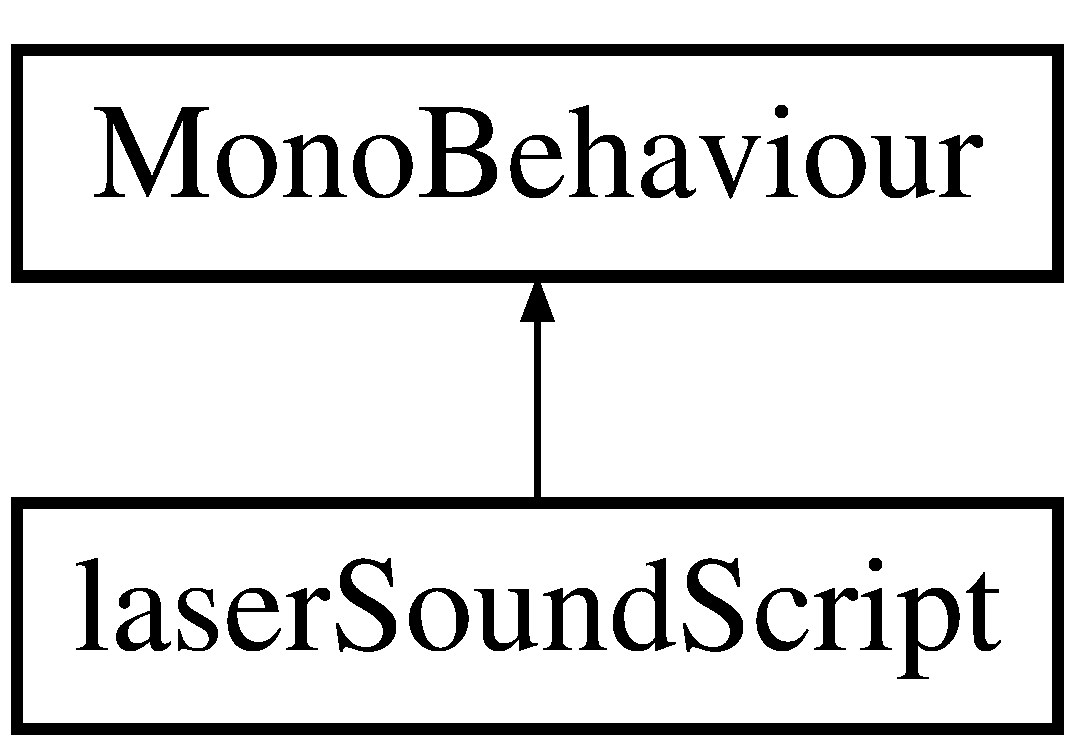
\includegraphics[height=2.000000cm]{classlaser_sound_script}
\end{center}
\end{figure}
\subsection*{Public Attributes}
\begin{DoxyCompactItemize}
\item 
bool \hyperlink{classlaser_sound_script_afb8896ad18029a39b23b03ac4ae7242b}{in\+Area}
\item 
Audio\+Source \hyperlink{classlaser_sound_script_aae195f857d34ee642da6b5cc5ffdf6c5}{laser}
\item 
\hyperlink{class_completion_script_four}{Completion\+Script\+Four} \hyperlink{classlaser_sound_script_a59d0d535475bebd3c0d0ea799c7e8e92}{turn\+Off}
\end{DoxyCompactItemize}


\subsection{Member Data Documentation}
\mbox{\Hypertarget{classlaser_sound_script_afb8896ad18029a39b23b03ac4ae7242b}\label{classlaser_sound_script_afb8896ad18029a39b23b03ac4ae7242b}} 
\index{laser\+Sound\+Script@{laser\+Sound\+Script}!in\+Area@{in\+Area}}
\index{in\+Area@{in\+Area}!laser\+Sound\+Script@{laser\+Sound\+Script}}
\subsubsection{\texorpdfstring{in\+Area}{inArea}}
{\footnotesize\ttfamily bool laser\+Sound\+Script.\+in\+Area}

\mbox{\Hypertarget{classlaser_sound_script_aae195f857d34ee642da6b5cc5ffdf6c5}\label{classlaser_sound_script_aae195f857d34ee642da6b5cc5ffdf6c5}} 
\index{laser\+Sound\+Script@{laser\+Sound\+Script}!laser@{laser}}
\index{laser@{laser}!laser\+Sound\+Script@{laser\+Sound\+Script}}
\subsubsection{\texorpdfstring{laser}{laser}}
{\footnotesize\ttfamily Audio\+Source laser\+Sound\+Script.\+laser}

\mbox{\Hypertarget{classlaser_sound_script_a59d0d535475bebd3c0d0ea799c7e8e92}\label{classlaser_sound_script_a59d0d535475bebd3c0d0ea799c7e8e92}} 
\index{laser\+Sound\+Script@{laser\+Sound\+Script}!turn\+Off@{turn\+Off}}
\index{turn\+Off@{turn\+Off}!laser\+Sound\+Script@{laser\+Sound\+Script}}
\subsubsection{\texorpdfstring{turn\+Off}{turnOff}}
{\footnotesize\ttfamily \hyperlink{class_completion_script_four}{Completion\+Script\+Four} laser\+Sound\+Script.\+turn\+Off}



The documentation for this class was generated from the following file\+:\begin{DoxyCompactItemize}
\item 
/\+Users/kwanholloway/git/5001\+Project/\+Game\+Project/\+Assets/\+Scripts/\+Game\+Logic/\hyperlink{laser_sound_script_8cs}{laser\+Sound\+Script.\+cs}\end{DoxyCompactItemize}

\hypertarget{class_left_laser_interaction}{}\section{Left\+Laser\+Interaction Class Reference}
\label{class_left_laser_interaction}\index{Left\+Laser\+Interaction@{Left\+Laser\+Interaction}}
Inheritance diagram for Left\+Laser\+Interaction\+:\begin{figure}[H]
\begin{center}
\leavevmode
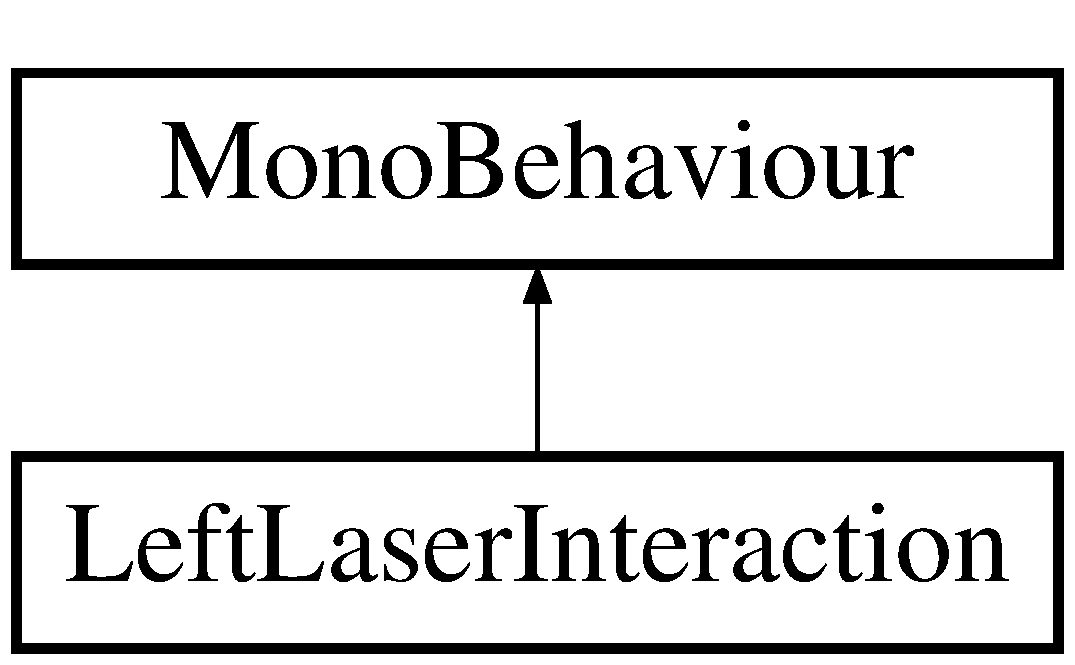
\includegraphics[height=2.000000cm]{class_left_laser_interaction}
\end{center}
\end{figure}
\subsection*{Public Attributes}
\begin{DoxyCompactItemize}
\item 
Text \hyperlink{class_left_laser_interaction_a275faec30b34227624a671a326ded543}{prompt}
\item 
Camera \hyperlink{class_left_laser_interaction_a08ffd3543f4374b6d08adb625756ce7e}{change\+Size}
\end{DoxyCompactItemize}


\subsection{Member Data Documentation}
\mbox{\Hypertarget{class_left_laser_interaction_a08ffd3543f4374b6d08adb625756ce7e}\label{class_left_laser_interaction_a08ffd3543f4374b6d08adb625756ce7e}} 
\index{Left\+Laser\+Interaction@{Left\+Laser\+Interaction}!change\+Size@{change\+Size}}
\index{change\+Size@{change\+Size}!Left\+Laser\+Interaction@{Left\+Laser\+Interaction}}
\subsubsection{\texorpdfstring{change\+Size}{changeSize}}
{\footnotesize\ttfamily Camera Left\+Laser\+Interaction.\+change\+Size}

\mbox{\Hypertarget{class_left_laser_interaction_a275faec30b34227624a671a326ded543}\label{class_left_laser_interaction_a275faec30b34227624a671a326ded543}} 
\index{Left\+Laser\+Interaction@{Left\+Laser\+Interaction}!prompt@{prompt}}
\index{prompt@{prompt}!Left\+Laser\+Interaction@{Left\+Laser\+Interaction}}
\subsubsection{\texorpdfstring{prompt}{prompt}}
{\footnotesize\ttfamily Text Left\+Laser\+Interaction.\+prompt}



The documentation for this class was generated from the following file\+:\begin{DoxyCompactItemize}
\item 
/\+Users/kwanholloway/git/5001\+Project/\+Game\+Project/\+Assets/\+Scripts/\+Z-\/\+N\+O\+T U\+S\+E\+D/\hyperlink{_left_laser_interaction_8cs}{Left\+Laser\+Interaction.\+cs}\end{DoxyCompactItemize}

\hypertarget{classlevel_complete_arith}{}\section{level\+Complete\+Arith Class Reference}
\label{classlevel_complete_arith}\index{level\+Complete\+Arith@{level\+Complete\+Arith}}
Inheritance diagram for level\+Complete\+Arith\+:\begin{figure}[H]
\begin{center}
\leavevmode
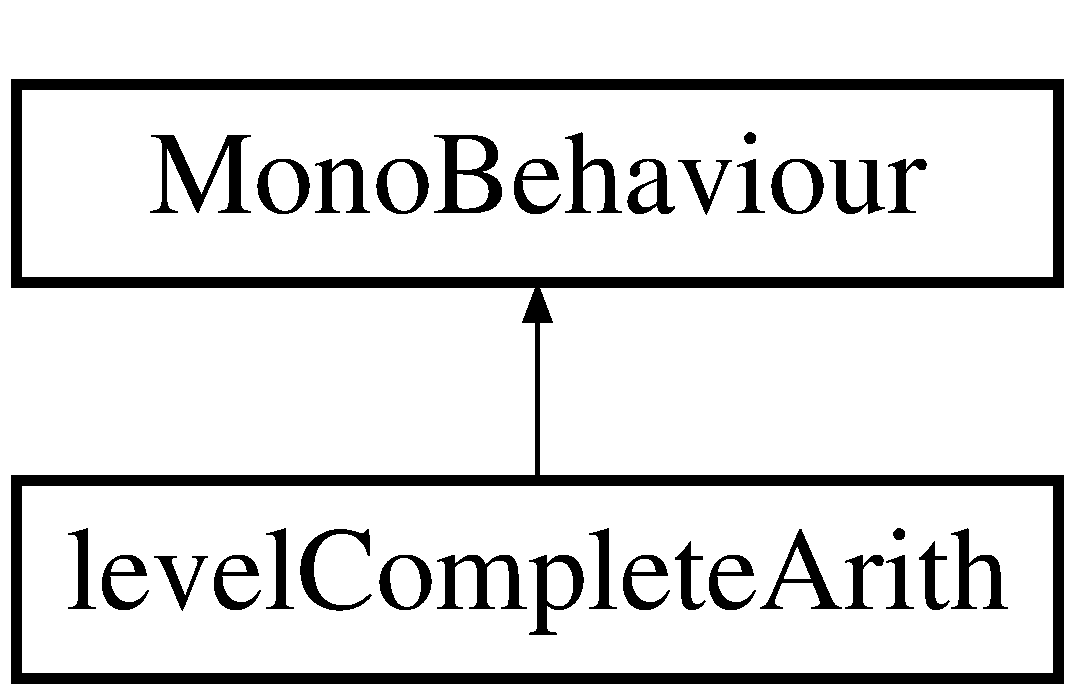
\includegraphics[height=2.000000cm]{classlevel_complete_arith}
\end{center}
\end{figure}
\subsection*{Public Attributes}
\begin{DoxyCompactItemize}
\item 
Game\+Object \mbox{[}$\,$\mbox{]} \hyperlink{classlevel_complete_arith_a821ae9580d37b6d88ada1cf8d816cca5}{level\+Complete\+Remove}
\end{DoxyCompactItemize}


\subsection{Member Data Documentation}
\mbox{\Hypertarget{classlevel_complete_arith_a821ae9580d37b6d88ada1cf8d816cca5}\label{classlevel_complete_arith_a821ae9580d37b6d88ada1cf8d816cca5}} 
\index{level\+Complete\+Arith@{level\+Complete\+Arith}!level\+Complete\+Remove@{level\+Complete\+Remove}}
\index{level\+Complete\+Remove@{level\+Complete\+Remove}!level\+Complete\+Arith@{level\+Complete\+Arith}}
\subsubsection{\texorpdfstring{level\+Complete\+Remove}{levelCompleteRemove}}
{\footnotesize\ttfamily Game\+Object \mbox{[}$\,$\mbox{]} level\+Complete\+Arith.\+level\+Complete\+Remove}



The documentation for this class was generated from the following file\+:\begin{DoxyCompactItemize}
\item 
/\+Users/kwanholloway/git/5001\+Project/\+Game\+Project/\+Assets/\hyperlink{level_complete_arith_8cs}{level\+Complete\+Arith.\+cs}\end{DoxyCompactItemize}

\hypertarget{classlevel_complete_array}{}\section{level\+Complete\+Array Class Reference}
\label{classlevel_complete_array}\index{level\+Complete\+Array@{level\+Complete\+Array}}
Inheritance diagram for level\+Complete\+Array\+:\begin{figure}[H]
\begin{center}
\leavevmode
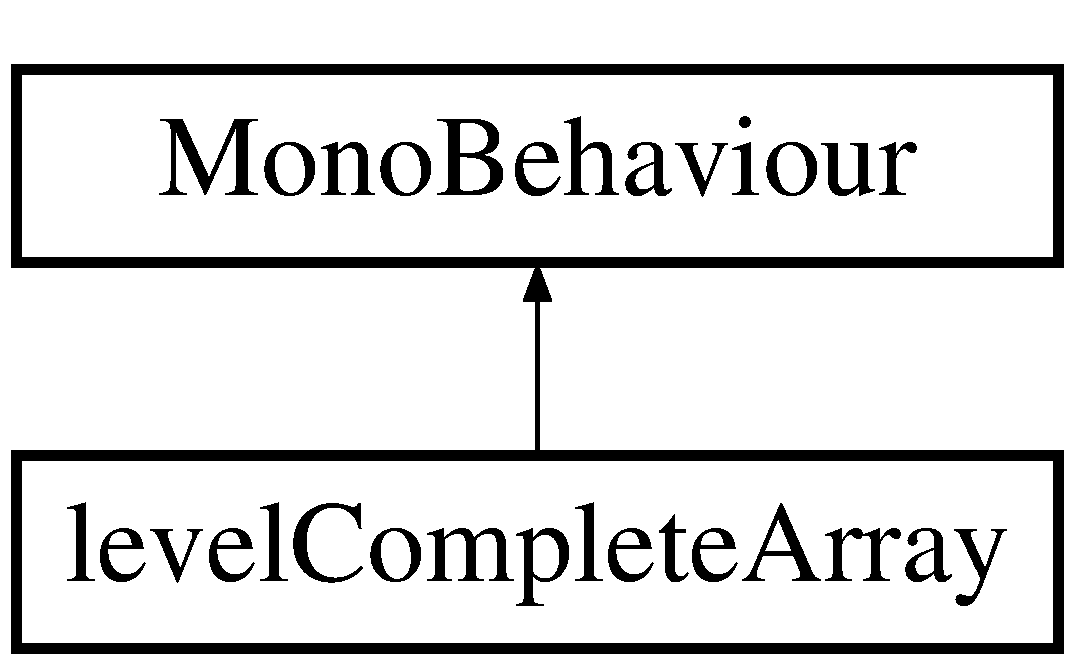
\includegraphics[height=2.000000cm]{classlevel_complete_array}
\end{center}
\end{figure}
\subsection*{Public Attributes}
\begin{DoxyCompactItemize}
\item 
Game\+Object \mbox{[}$\,$\mbox{]} \hyperlink{classlevel_complete_array_a24b83f2696ca2c65b1412047a618f49b}{level\+Complete\+Remove}
\end{DoxyCompactItemize}


\subsection{Member Data Documentation}
\mbox{\Hypertarget{classlevel_complete_array_a24b83f2696ca2c65b1412047a618f49b}\label{classlevel_complete_array_a24b83f2696ca2c65b1412047a618f49b}} 
\index{level\+Complete\+Array@{level\+Complete\+Array}!level\+Complete\+Remove@{level\+Complete\+Remove}}
\index{level\+Complete\+Remove@{level\+Complete\+Remove}!level\+Complete\+Array@{level\+Complete\+Array}}
\subsubsection{\texorpdfstring{level\+Complete\+Remove}{levelCompleteRemove}}
{\footnotesize\ttfamily Game\+Object \mbox{[}$\,$\mbox{]} level\+Complete\+Array.\+level\+Complete\+Remove}



The documentation for this class was generated from the following file\+:\begin{DoxyCompactItemize}
\item 
/\+Users/kwanholloway/git/5001\+Project/\+Game\+Project/\+Assets/\+Scripts/\hyperlink{level_complete_array_8cs}{level\+Complete\+Array.\+cs}\end{DoxyCompactItemize}

\hypertarget{classlevel_complete_cond}{}\section{level\+Complete\+Cond Class Reference}
\label{classlevel_complete_cond}\index{level\+Complete\+Cond@{level\+Complete\+Cond}}
Inheritance diagram for level\+Complete\+Cond\+:\begin{figure}[H]
\begin{center}
\leavevmode
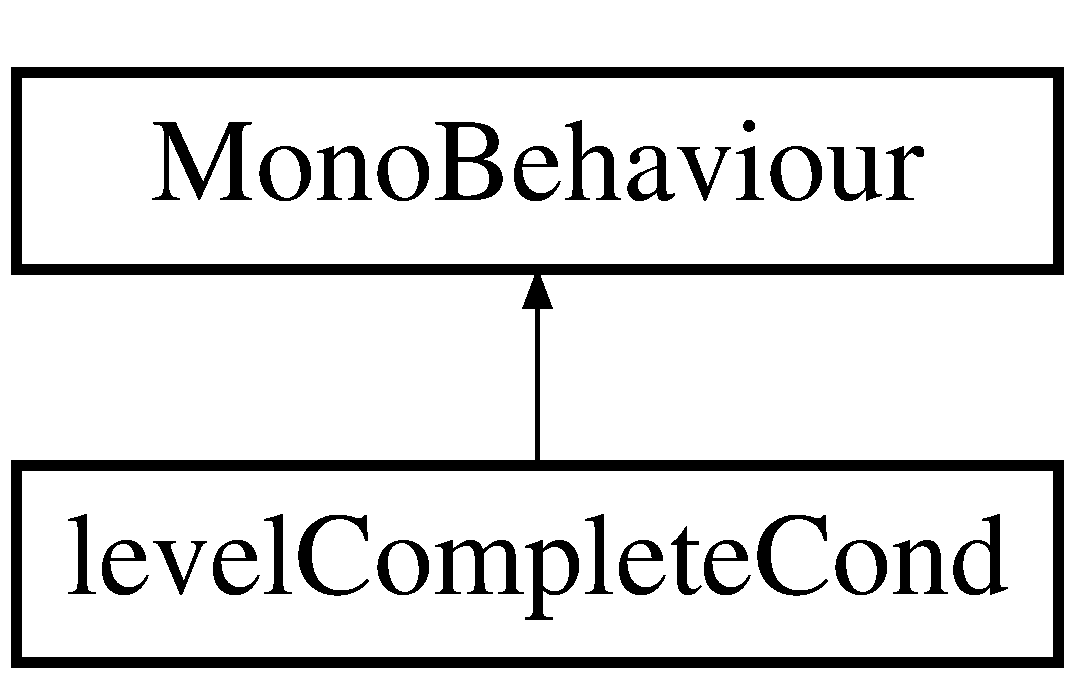
\includegraphics[height=2.000000cm]{classlevel_complete_cond}
\end{center}
\end{figure}
\subsection*{Public Attributes}
\begin{DoxyCompactItemize}
\item 
Game\+Object \mbox{[}$\,$\mbox{]} \hyperlink{classlevel_complete_cond_adf0e456569f3f5ccd52212147e98f743}{level\+Complete\+Remove}
\end{DoxyCompactItemize}


\subsection{Member Data Documentation}
\mbox{\Hypertarget{classlevel_complete_cond_adf0e456569f3f5ccd52212147e98f743}\label{classlevel_complete_cond_adf0e456569f3f5ccd52212147e98f743}} 
\index{level\+Complete\+Cond@{level\+Complete\+Cond}!level\+Complete\+Remove@{level\+Complete\+Remove}}
\index{level\+Complete\+Remove@{level\+Complete\+Remove}!level\+Complete\+Cond@{level\+Complete\+Cond}}
\subsubsection{\texorpdfstring{level\+Complete\+Remove}{levelCompleteRemove}}
{\footnotesize\ttfamily Game\+Object \mbox{[}$\,$\mbox{]} level\+Complete\+Cond.\+level\+Complete\+Remove}



The documentation for this class was generated from the following file\+:\begin{DoxyCompactItemize}
\item 
/\+Users/kwanholloway/git/5001\+Project/\+Game\+Project/\+Assets/\hyperlink{level_complete_cond_8cs}{level\+Complete\+Cond.\+cs}\end{DoxyCompactItemize}

\hypertarget{classlevel_complete_loop}{}\section{level\+Complete\+Loop Class Reference}
\label{classlevel_complete_loop}\index{level\+Complete\+Loop@{level\+Complete\+Loop}}
Inheritance diagram for level\+Complete\+Loop\+:\begin{figure}[H]
\begin{center}
\leavevmode
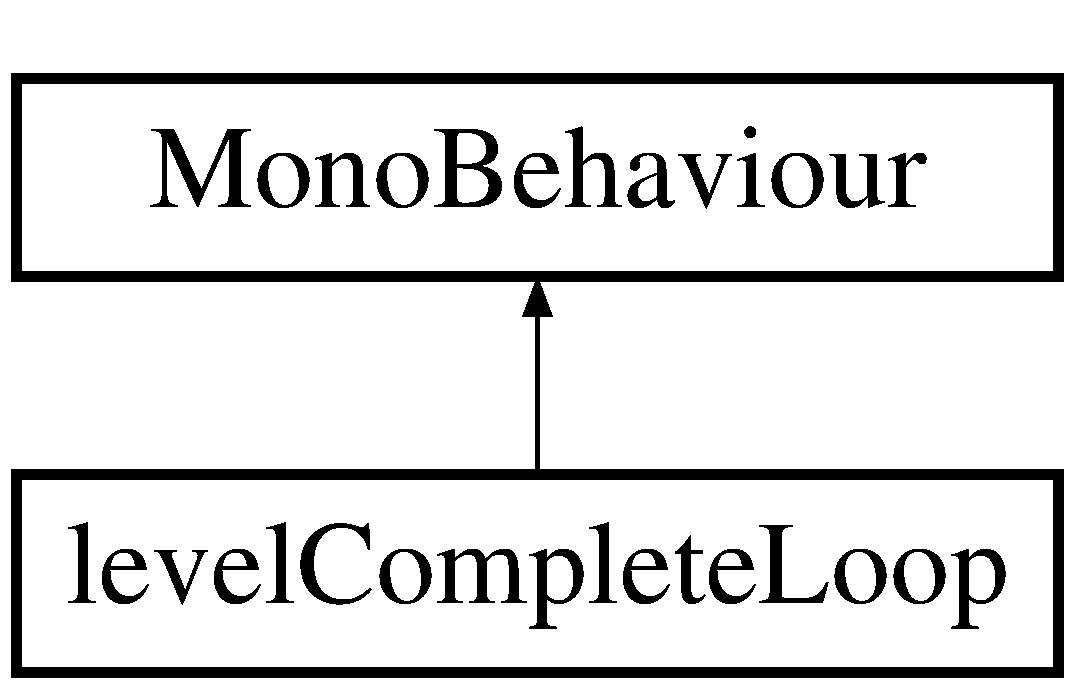
\includegraphics[height=2.000000cm]{classlevel_complete_loop}
\end{center}
\end{figure}
\subsection*{Public Attributes}
\begin{DoxyCompactItemize}
\item 
Game\+Object \mbox{[}$\,$\mbox{]} \hyperlink{classlevel_complete_loop_adfbef5a438c566c7762842f7d5102b67}{level\+Complete\+Remove}
\end{DoxyCompactItemize}


\subsection{Member Data Documentation}
\mbox{\Hypertarget{classlevel_complete_loop_adfbef5a438c566c7762842f7d5102b67}\label{classlevel_complete_loop_adfbef5a438c566c7762842f7d5102b67}} 
\index{level\+Complete\+Loop@{level\+Complete\+Loop}!level\+Complete\+Remove@{level\+Complete\+Remove}}
\index{level\+Complete\+Remove@{level\+Complete\+Remove}!level\+Complete\+Loop@{level\+Complete\+Loop}}
\subsubsection{\texorpdfstring{level\+Complete\+Remove}{levelCompleteRemove}}
{\footnotesize\ttfamily Game\+Object \mbox{[}$\,$\mbox{]} level\+Complete\+Loop.\+level\+Complete\+Remove}



The documentation for this class was generated from the following file\+:\begin{DoxyCompactItemize}
\item 
/\+Users/kwanholloway/git/5001\+Project/\+Game\+Project/\+Assets/\+Scripts/\hyperlink{level_complete_loop_8cs}{level\+Complete\+Loop.\+cs}\end{DoxyCompactItemize}

\hypertarget{class_logical_and_completion}{}\section{Logical\+And\+Completion Class Reference}
\label{class_logical_and_completion}\index{Logical\+And\+Completion@{Logical\+And\+Completion}}
Inheritance diagram for Logical\+And\+Completion\+:\begin{figure}[H]
\begin{center}
\leavevmode
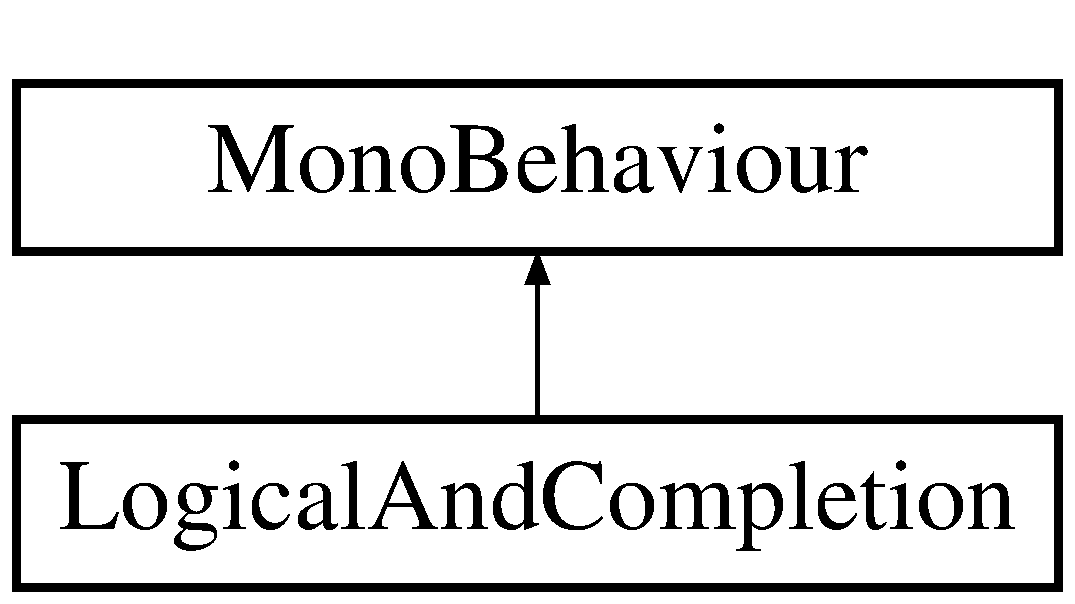
\includegraphics[height=2.000000cm]{class_logical_and_completion}
\end{center}
\end{figure}
\subsection*{Public Member Functions}
\begin{DoxyCompactItemize}
\item 
void \hyperlink{class_logical_and_completion_a9ed46f831997831283dfd2d8c35d58f9}{reset\+Puzzle} ()
\item 
void \hyperlink{class_logical_and_completion_a6474fb7522f26a6cc7a0a5ce3965fffd}{control\+Left} ()
\item 
void \hyperlink{class_logical_and_completion_a4598f8cd0da38a1ebb2feae2c325f15e}{control\+Right} ()
\item 
void \hyperlink{class_logical_and_completion_aea21ae98d9ca7f00d198c50e176b74eb}{reset\+Pylon} ()
\item 
void \hyperlink{class_logical_and_completion_ac840b6d7276acb039cd91beca9a17130}{reset\+Check\+Values} ()
\item 
void \hyperlink{class_logical_and_completion_af6f46bed91d1c88a40caa1483cb8d67e}{reset\+Slots} ()
\item 
void \hyperlink{class_logical_and_completion_a6a6d723a0e8ecbb8d5c034a0f05748f8}{reset\+Tiles} ()
\item 
void \hyperlink{class_logical_and_completion_ac0555b8b727d4521aa4b469e3a76c74a}{reset\+Active} ()
\end{DoxyCompactItemize}
\subsection*{Public Attributes}
\begin{DoxyCompactItemize}
\item 
\hyperlink{class_array_reaction}{Array\+Reaction} \hyperlink{class_logical_and_completion_a7ed4ecdaf29b98fa3264c51a64eb726e}{slot\+One\+Success}
\item 
\hyperlink{class_array_reaction}{Array\+Reaction} \hyperlink{class_logical_and_completion_a925f99929d6fe0f68f245914fb0e1e95}{replacement\+True}
\item 
bool \hyperlink{class_logical_and_completion_a5bff7c897b4ebfca7d56e238917de8e4}{puzzle\+Finished}
\item 
Game\+Object \mbox{[}$\,$\mbox{]} \hyperlink{class_logical_and_completion_a1d6d43ba546c81e5b9c5cda3837be009}{array\+Tiles}
\item 
Game\+Object \mbox{[}$\,$\mbox{]} \hyperlink{class_logical_and_completion_a9dd15007bbc76569e7c82904c2464124}{replacement\+Tiles}
\item 
Game\+Object \hyperlink{class_logical_and_completion_af6e487086d828fe81dc8890754f32c38}{left\+Pylon\+Closed}
\item 
Game\+Object \hyperlink{class_logical_and_completion_ad50f71a4157df3e8ca40c98eada1d3fb}{right\+Pylon\+Closed}
\item 
Game\+Object \hyperlink{class_logical_and_completion_a803aec34894a6af536b64611019c6372}{left\+Pylon\+Raised}
\item 
Game\+Object \hyperlink{class_logical_and_completion_a49166cfb32e7409ba04133c408d47793}{right\+Pylon\+Raised}
\item 
Game\+Object \hyperlink{class_logical_and_completion_a95b8a1803a7ce81d2d45f88b036e7f9e}{door\+One}
\item 
Audio\+Source \hyperlink{class_logical_and_completion_a2cf6ce1f33f9c648fa21cb6b97e785b3}{solved}
\end{DoxyCompactItemize}


\subsection{Member Function Documentation}
\mbox{\Hypertarget{class_logical_and_completion_a6474fb7522f26a6cc7a0a5ce3965fffd}\label{class_logical_and_completion_a6474fb7522f26a6cc7a0a5ce3965fffd}} 
\index{Logical\+And\+Completion@{Logical\+And\+Completion}!control\+Left@{control\+Left}}
\index{control\+Left@{control\+Left}!Logical\+And\+Completion@{Logical\+And\+Completion}}
\subsubsection{\texorpdfstring{control\+Left()}{controlLeft()}}
{\footnotesize\ttfamily void Logical\+And\+Completion.\+control\+Left (\begin{DoxyParamCaption}{ }\end{DoxyParamCaption})}

\mbox{\Hypertarget{class_logical_and_completion_a4598f8cd0da38a1ebb2feae2c325f15e}\label{class_logical_and_completion_a4598f8cd0da38a1ebb2feae2c325f15e}} 
\index{Logical\+And\+Completion@{Logical\+And\+Completion}!control\+Right@{control\+Right}}
\index{control\+Right@{control\+Right}!Logical\+And\+Completion@{Logical\+And\+Completion}}
\subsubsection{\texorpdfstring{control\+Right()}{controlRight()}}
{\footnotesize\ttfamily void Logical\+And\+Completion.\+control\+Right (\begin{DoxyParamCaption}{ }\end{DoxyParamCaption})}

\mbox{\Hypertarget{class_logical_and_completion_ac0555b8b727d4521aa4b469e3a76c74a}\label{class_logical_and_completion_ac0555b8b727d4521aa4b469e3a76c74a}} 
\index{Logical\+And\+Completion@{Logical\+And\+Completion}!reset\+Active@{reset\+Active}}
\index{reset\+Active@{reset\+Active}!Logical\+And\+Completion@{Logical\+And\+Completion}}
\subsubsection{\texorpdfstring{reset\+Active()}{resetActive()}}
{\footnotesize\ttfamily void Logical\+And\+Completion.\+reset\+Active (\begin{DoxyParamCaption}{ }\end{DoxyParamCaption})}

\mbox{\Hypertarget{class_logical_and_completion_ac840b6d7276acb039cd91beca9a17130}\label{class_logical_and_completion_ac840b6d7276acb039cd91beca9a17130}} 
\index{Logical\+And\+Completion@{Logical\+And\+Completion}!reset\+Check\+Values@{reset\+Check\+Values}}
\index{reset\+Check\+Values@{reset\+Check\+Values}!Logical\+And\+Completion@{Logical\+And\+Completion}}
\subsubsection{\texorpdfstring{reset\+Check\+Values()}{resetCheckValues()}}
{\footnotesize\ttfamily void Logical\+And\+Completion.\+reset\+Check\+Values (\begin{DoxyParamCaption}{ }\end{DoxyParamCaption})}

\mbox{\Hypertarget{class_logical_and_completion_a9ed46f831997831283dfd2d8c35d58f9}\label{class_logical_and_completion_a9ed46f831997831283dfd2d8c35d58f9}} 
\index{Logical\+And\+Completion@{Logical\+And\+Completion}!reset\+Puzzle@{reset\+Puzzle}}
\index{reset\+Puzzle@{reset\+Puzzle}!Logical\+And\+Completion@{Logical\+And\+Completion}}
\subsubsection{\texorpdfstring{reset\+Puzzle()}{resetPuzzle()}}
{\footnotesize\ttfamily void Logical\+And\+Completion.\+reset\+Puzzle (\begin{DoxyParamCaption}{ }\end{DoxyParamCaption})}

\mbox{\Hypertarget{class_logical_and_completion_aea21ae98d9ca7f00d198c50e176b74eb}\label{class_logical_and_completion_aea21ae98d9ca7f00d198c50e176b74eb}} 
\index{Logical\+And\+Completion@{Logical\+And\+Completion}!reset\+Pylon@{reset\+Pylon}}
\index{reset\+Pylon@{reset\+Pylon}!Logical\+And\+Completion@{Logical\+And\+Completion}}
\subsubsection{\texorpdfstring{reset\+Pylon()}{resetPylon()}}
{\footnotesize\ttfamily void Logical\+And\+Completion.\+reset\+Pylon (\begin{DoxyParamCaption}{ }\end{DoxyParamCaption})}

\mbox{\Hypertarget{class_logical_and_completion_af6f46bed91d1c88a40caa1483cb8d67e}\label{class_logical_and_completion_af6f46bed91d1c88a40caa1483cb8d67e}} 
\index{Logical\+And\+Completion@{Logical\+And\+Completion}!reset\+Slots@{reset\+Slots}}
\index{reset\+Slots@{reset\+Slots}!Logical\+And\+Completion@{Logical\+And\+Completion}}
\subsubsection{\texorpdfstring{reset\+Slots()}{resetSlots()}}
{\footnotesize\ttfamily void Logical\+And\+Completion.\+reset\+Slots (\begin{DoxyParamCaption}{ }\end{DoxyParamCaption})}

\mbox{\Hypertarget{class_logical_and_completion_a6a6d723a0e8ecbb8d5c034a0f05748f8}\label{class_logical_and_completion_a6a6d723a0e8ecbb8d5c034a0f05748f8}} 
\index{Logical\+And\+Completion@{Logical\+And\+Completion}!reset\+Tiles@{reset\+Tiles}}
\index{reset\+Tiles@{reset\+Tiles}!Logical\+And\+Completion@{Logical\+And\+Completion}}
\subsubsection{\texorpdfstring{reset\+Tiles()}{resetTiles()}}
{\footnotesize\ttfamily void Logical\+And\+Completion.\+reset\+Tiles (\begin{DoxyParamCaption}{ }\end{DoxyParamCaption})}



\subsection{Member Data Documentation}
\mbox{\Hypertarget{class_logical_and_completion_a1d6d43ba546c81e5b9c5cda3837be009}\label{class_logical_and_completion_a1d6d43ba546c81e5b9c5cda3837be009}} 
\index{Logical\+And\+Completion@{Logical\+And\+Completion}!array\+Tiles@{array\+Tiles}}
\index{array\+Tiles@{array\+Tiles}!Logical\+And\+Completion@{Logical\+And\+Completion}}
\subsubsection{\texorpdfstring{array\+Tiles}{arrayTiles}}
{\footnotesize\ttfamily Game\+Object \mbox{[}$\,$\mbox{]} Logical\+And\+Completion.\+array\+Tiles}

\mbox{\Hypertarget{class_logical_and_completion_a95b8a1803a7ce81d2d45f88b036e7f9e}\label{class_logical_and_completion_a95b8a1803a7ce81d2d45f88b036e7f9e}} 
\index{Logical\+And\+Completion@{Logical\+And\+Completion}!door\+One@{door\+One}}
\index{door\+One@{door\+One}!Logical\+And\+Completion@{Logical\+And\+Completion}}
\subsubsection{\texorpdfstring{door\+One}{doorOne}}
{\footnotesize\ttfamily Game\+Object Logical\+And\+Completion.\+door\+One}

\mbox{\Hypertarget{class_logical_and_completion_af6e487086d828fe81dc8890754f32c38}\label{class_logical_and_completion_af6e487086d828fe81dc8890754f32c38}} 
\index{Logical\+And\+Completion@{Logical\+And\+Completion}!left\+Pylon\+Closed@{left\+Pylon\+Closed}}
\index{left\+Pylon\+Closed@{left\+Pylon\+Closed}!Logical\+And\+Completion@{Logical\+And\+Completion}}
\subsubsection{\texorpdfstring{left\+Pylon\+Closed}{leftPylonClosed}}
{\footnotesize\ttfamily Game\+Object Logical\+And\+Completion.\+left\+Pylon\+Closed}

\mbox{\Hypertarget{class_logical_and_completion_a803aec34894a6af536b64611019c6372}\label{class_logical_and_completion_a803aec34894a6af536b64611019c6372}} 
\index{Logical\+And\+Completion@{Logical\+And\+Completion}!left\+Pylon\+Raised@{left\+Pylon\+Raised}}
\index{left\+Pylon\+Raised@{left\+Pylon\+Raised}!Logical\+And\+Completion@{Logical\+And\+Completion}}
\subsubsection{\texorpdfstring{left\+Pylon\+Raised}{leftPylonRaised}}
{\footnotesize\ttfamily Game\+Object Logical\+And\+Completion.\+left\+Pylon\+Raised}

\mbox{\Hypertarget{class_logical_and_completion_a5bff7c897b4ebfca7d56e238917de8e4}\label{class_logical_and_completion_a5bff7c897b4ebfca7d56e238917de8e4}} 
\index{Logical\+And\+Completion@{Logical\+And\+Completion}!puzzle\+Finished@{puzzle\+Finished}}
\index{puzzle\+Finished@{puzzle\+Finished}!Logical\+And\+Completion@{Logical\+And\+Completion}}
\subsubsection{\texorpdfstring{puzzle\+Finished}{puzzleFinished}}
{\footnotesize\ttfamily bool Logical\+And\+Completion.\+puzzle\+Finished}

\mbox{\Hypertarget{class_logical_and_completion_a9dd15007bbc76569e7c82904c2464124}\label{class_logical_and_completion_a9dd15007bbc76569e7c82904c2464124}} 
\index{Logical\+And\+Completion@{Logical\+And\+Completion}!replacement\+Tiles@{replacement\+Tiles}}
\index{replacement\+Tiles@{replacement\+Tiles}!Logical\+And\+Completion@{Logical\+And\+Completion}}
\subsubsection{\texorpdfstring{replacement\+Tiles}{replacementTiles}}
{\footnotesize\ttfamily Game\+Object \mbox{[}$\,$\mbox{]} Logical\+And\+Completion.\+replacement\+Tiles}

\mbox{\Hypertarget{class_logical_and_completion_a925f99929d6fe0f68f245914fb0e1e95}\label{class_logical_and_completion_a925f99929d6fe0f68f245914fb0e1e95}} 
\index{Logical\+And\+Completion@{Logical\+And\+Completion}!replacement\+True@{replacement\+True}}
\index{replacement\+True@{replacement\+True}!Logical\+And\+Completion@{Logical\+And\+Completion}}
\subsubsection{\texorpdfstring{replacement\+True}{replacementTrue}}
{\footnotesize\ttfamily \hyperlink{class_array_reaction}{Array\+Reaction} Logical\+And\+Completion.\+replacement\+True}

\mbox{\Hypertarget{class_logical_and_completion_ad50f71a4157df3e8ca40c98eada1d3fb}\label{class_logical_and_completion_ad50f71a4157df3e8ca40c98eada1d3fb}} 
\index{Logical\+And\+Completion@{Logical\+And\+Completion}!right\+Pylon\+Closed@{right\+Pylon\+Closed}}
\index{right\+Pylon\+Closed@{right\+Pylon\+Closed}!Logical\+And\+Completion@{Logical\+And\+Completion}}
\subsubsection{\texorpdfstring{right\+Pylon\+Closed}{rightPylonClosed}}
{\footnotesize\ttfamily Game\+Object Logical\+And\+Completion.\+right\+Pylon\+Closed}

\mbox{\Hypertarget{class_logical_and_completion_a49166cfb32e7409ba04133c408d47793}\label{class_logical_and_completion_a49166cfb32e7409ba04133c408d47793}} 
\index{Logical\+And\+Completion@{Logical\+And\+Completion}!right\+Pylon\+Raised@{right\+Pylon\+Raised}}
\index{right\+Pylon\+Raised@{right\+Pylon\+Raised}!Logical\+And\+Completion@{Logical\+And\+Completion}}
\subsubsection{\texorpdfstring{right\+Pylon\+Raised}{rightPylonRaised}}
{\footnotesize\ttfamily Game\+Object Logical\+And\+Completion.\+right\+Pylon\+Raised}

\mbox{\Hypertarget{class_logical_and_completion_a7ed4ecdaf29b98fa3264c51a64eb726e}\label{class_logical_and_completion_a7ed4ecdaf29b98fa3264c51a64eb726e}} 
\index{Logical\+And\+Completion@{Logical\+And\+Completion}!slot\+One\+Success@{slot\+One\+Success}}
\index{slot\+One\+Success@{slot\+One\+Success}!Logical\+And\+Completion@{Logical\+And\+Completion}}
\subsubsection{\texorpdfstring{slot\+One\+Success}{slotOneSuccess}}
{\footnotesize\ttfamily \hyperlink{class_array_reaction}{Array\+Reaction} Logical\+And\+Completion.\+slot\+One\+Success}

\mbox{\Hypertarget{class_logical_and_completion_a2cf6ce1f33f9c648fa21cb6b97e785b3}\label{class_logical_and_completion_a2cf6ce1f33f9c648fa21cb6b97e785b3}} 
\index{Logical\+And\+Completion@{Logical\+And\+Completion}!solved@{solved}}
\index{solved@{solved}!Logical\+And\+Completion@{Logical\+And\+Completion}}
\subsubsection{\texorpdfstring{solved}{solved}}
{\footnotesize\ttfamily Audio\+Source Logical\+And\+Completion.\+solved}



The documentation for this class was generated from the following file\+:\begin{DoxyCompactItemize}
\item 
/\+Users/kwanholloway/git/5001\+Project/\+Game\+Project/\+Assets/\+Scripts/\+Puzzle\+Logic/\+Conditional Level/\hyperlink{_logical_and_completion_8cs}{Logical\+And\+Completion.\+cs}\end{DoxyCompactItemize}

\hypertarget{class_logical_or_completion}{}\section{Logical\+Or\+Completion Class Reference}
\label{class_logical_or_completion}\index{Logical\+Or\+Completion@{Logical\+Or\+Completion}}
Inheritance diagram for Logical\+Or\+Completion\+:\begin{figure}[H]
\begin{center}
\leavevmode
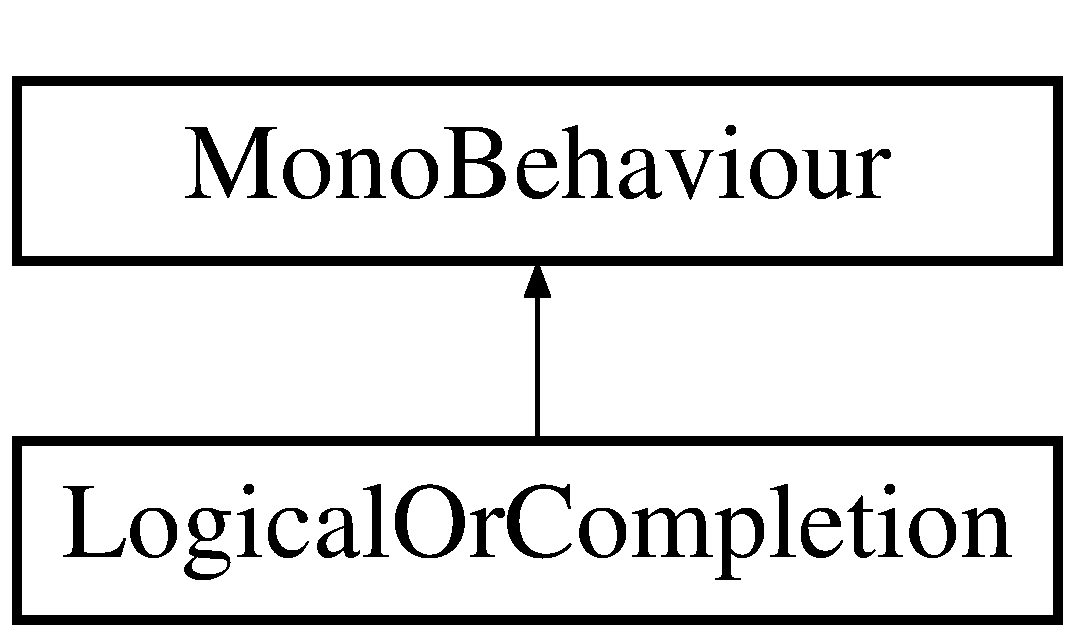
\includegraphics[height=2.000000cm]{class_logical_or_completion}
\end{center}
\end{figure}
\subsection*{Public Member Functions}
\begin{DoxyCompactItemize}
\item 
void \hyperlink{class_logical_or_completion_a783c46d26a4f12f44b04b03863f42d95}{reset\+Puzzle} ()
\item 
void \hyperlink{class_logical_or_completion_af8cbd9a832c9c69ee46fb70020a7989b}{control\+Left} ()
\item 
void \hyperlink{class_logical_or_completion_a782b87c3afba79cbc18d704ab3583540}{control\+Right} ()
\item 
void \hyperlink{class_logical_or_completion_a250f9585b961379f94d16a564eec723a}{reset\+Pylon} ()
\item 
void \hyperlink{class_logical_or_completion_ac6b1be85673c5739f7eacd97f1811964}{reset\+Check\+Values} ()
\item 
void \hyperlink{class_logical_or_completion_a55e66d307bb74dbd3891e93a48d88131}{reset\+Slots} ()
\item 
void \hyperlink{class_logical_or_completion_abeb657802f2f8f3f6e768ca10bacfdb6}{reset\+Tiles} ()
\item 
void \hyperlink{class_logical_or_completion_a7a4f4c9e3a2b79189a21fefb8a81f919}{reset\+Active} ()
\end{DoxyCompactItemize}
\subsection*{Public Attributes}
\begin{DoxyCompactItemize}
\item 
\hyperlink{class_array_reaction}{Array\+Reaction} \hyperlink{class_logical_or_completion_ae5240c050cf760aca98a3466dfa3bd6a}{true\+Success}
\item 
\hyperlink{class_array_reaction}{Array\+Reaction} \hyperlink{class_logical_or_completion_aabb4ebdcb4e38046c43f6379d7c0b688}{replacement\+True}
\item 
bool \hyperlink{class_logical_or_completion_ad518cbefee91205d37240ba2dd7fdd19}{puzzle\+Finished}
\item 
Game\+Object \mbox{[}$\,$\mbox{]} \hyperlink{class_logical_or_completion_a5a9d2e3e6a922a095361ab66a2e1342e}{array\+Tiles}
\item 
Game\+Object \mbox{[}$\,$\mbox{]} \hyperlink{class_logical_or_completion_a4a8bfa05984877d32f5575d0bab00e1d}{replacement\+Tiles}
\item 
Game\+Object \hyperlink{class_logical_or_completion_a5618b9b7c564da318010746ba2a081d4}{left\+Pylon\+Closed}
\item 
Game\+Object \hyperlink{class_logical_or_completion_af7cfc7e6435c297479a2bcb47481ae59}{right\+Pylon\+Closed}
\item 
Game\+Object \hyperlink{class_logical_or_completion_adeb8fe88dd74a1b439ada910c58d0ae3}{left\+Pylon\+Raised}
\item 
Game\+Object \hyperlink{class_logical_or_completion_ae7398a003db47542eed166c249a78ee2}{right\+Pylon\+Raised}
\item 
Game\+Object \hyperlink{class_logical_or_completion_a0143c2b8f5eca58b7a3606c281381c9b}{door\+One}
\item 
Audio\+Source \hyperlink{class_logical_or_completion_a5c9e98e9b0cdfe29a2ed689a6d2da120}{solved}
\end{DoxyCompactItemize}


\subsection{Member Function Documentation}
\mbox{\Hypertarget{class_logical_or_completion_af8cbd9a832c9c69ee46fb70020a7989b}\label{class_logical_or_completion_af8cbd9a832c9c69ee46fb70020a7989b}} 
\index{Logical\+Or\+Completion@{Logical\+Or\+Completion}!control\+Left@{control\+Left}}
\index{control\+Left@{control\+Left}!Logical\+Or\+Completion@{Logical\+Or\+Completion}}
\subsubsection{\texorpdfstring{control\+Left()}{controlLeft()}}
{\footnotesize\ttfamily void Logical\+Or\+Completion.\+control\+Left (\begin{DoxyParamCaption}{ }\end{DoxyParamCaption})}

\mbox{\Hypertarget{class_logical_or_completion_a782b87c3afba79cbc18d704ab3583540}\label{class_logical_or_completion_a782b87c3afba79cbc18d704ab3583540}} 
\index{Logical\+Or\+Completion@{Logical\+Or\+Completion}!control\+Right@{control\+Right}}
\index{control\+Right@{control\+Right}!Logical\+Or\+Completion@{Logical\+Or\+Completion}}
\subsubsection{\texorpdfstring{control\+Right()}{controlRight()}}
{\footnotesize\ttfamily void Logical\+Or\+Completion.\+control\+Right (\begin{DoxyParamCaption}{ }\end{DoxyParamCaption})}

\mbox{\Hypertarget{class_logical_or_completion_a7a4f4c9e3a2b79189a21fefb8a81f919}\label{class_logical_or_completion_a7a4f4c9e3a2b79189a21fefb8a81f919}} 
\index{Logical\+Or\+Completion@{Logical\+Or\+Completion}!reset\+Active@{reset\+Active}}
\index{reset\+Active@{reset\+Active}!Logical\+Or\+Completion@{Logical\+Or\+Completion}}
\subsubsection{\texorpdfstring{reset\+Active()}{resetActive()}}
{\footnotesize\ttfamily void Logical\+Or\+Completion.\+reset\+Active (\begin{DoxyParamCaption}{ }\end{DoxyParamCaption})}

\mbox{\Hypertarget{class_logical_or_completion_ac6b1be85673c5739f7eacd97f1811964}\label{class_logical_or_completion_ac6b1be85673c5739f7eacd97f1811964}} 
\index{Logical\+Or\+Completion@{Logical\+Or\+Completion}!reset\+Check\+Values@{reset\+Check\+Values}}
\index{reset\+Check\+Values@{reset\+Check\+Values}!Logical\+Or\+Completion@{Logical\+Or\+Completion}}
\subsubsection{\texorpdfstring{reset\+Check\+Values()}{resetCheckValues()}}
{\footnotesize\ttfamily void Logical\+Or\+Completion.\+reset\+Check\+Values (\begin{DoxyParamCaption}{ }\end{DoxyParamCaption})}

\mbox{\Hypertarget{class_logical_or_completion_a783c46d26a4f12f44b04b03863f42d95}\label{class_logical_or_completion_a783c46d26a4f12f44b04b03863f42d95}} 
\index{Logical\+Or\+Completion@{Logical\+Or\+Completion}!reset\+Puzzle@{reset\+Puzzle}}
\index{reset\+Puzzle@{reset\+Puzzle}!Logical\+Or\+Completion@{Logical\+Or\+Completion}}
\subsubsection{\texorpdfstring{reset\+Puzzle()}{resetPuzzle()}}
{\footnotesize\ttfamily void Logical\+Or\+Completion.\+reset\+Puzzle (\begin{DoxyParamCaption}{ }\end{DoxyParamCaption})}

\mbox{\Hypertarget{class_logical_or_completion_a250f9585b961379f94d16a564eec723a}\label{class_logical_or_completion_a250f9585b961379f94d16a564eec723a}} 
\index{Logical\+Or\+Completion@{Logical\+Or\+Completion}!reset\+Pylon@{reset\+Pylon}}
\index{reset\+Pylon@{reset\+Pylon}!Logical\+Or\+Completion@{Logical\+Or\+Completion}}
\subsubsection{\texorpdfstring{reset\+Pylon()}{resetPylon()}}
{\footnotesize\ttfamily void Logical\+Or\+Completion.\+reset\+Pylon (\begin{DoxyParamCaption}{ }\end{DoxyParamCaption})}

\mbox{\Hypertarget{class_logical_or_completion_a55e66d307bb74dbd3891e93a48d88131}\label{class_logical_or_completion_a55e66d307bb74dbd3891e93a48d88131}} 
\index{Logical\+Or\+Completion@{Logical\+Or\+Completion}!reset\+Slots@{reset\+Slots}}
\index{reset\+Slots@{reset\+Slots}!Logical\+Or\+Completion@{Logical\+Or\+Completion}}
\subsubsection{\texorpdfstring{reset\+Slots()}{resetSlots()}}
{\footnotesize\ttfamily void Logical\+Or\+Completion.\+reset\+Slots (\begin{DoxyParamCaption}{ }\end{DoxyParamCaption})}

\mbox{\Hypertarget{class_logical_or_completion_abeb657802f2f8f3f6e768ca10bacfdb6}\label{class_logical_or_completion_abeb657802f2f8f3f6e768ca10bacfdb6}} 
\index{Logical\+Or\+Completion@{Logical\+Or\+Completion}!reset\+Tiles@{reset\+Tiles}}
\index{reset\+Tiles@{reset\+Tiles}!Logical\+Or\+Completion@{Logical\+Or\+Completion}}
\subsubsection{\texorpdfstring{reset\+Tiles()}{resetTiles()}}
{\footnotesize\ttfamily void Logical\+Or\+Completion.\+reset\+Tiles (\begin{DoxyParamCaption}{ }\end{DoxyParamCaption})}



\subsection{Member Data Documentation}
\mbox{\Hypertarget{class_logical_or_completion_a5a9d2e3e6a922a095361ab66a2e1342e}\label{class_logical_or_completion_a5a9d2e3e6a922a095361ab66a2e1342e}} 
\index{Logical\+Or\+Completion@{Logical\+Or\+Completion}!array\+Tiles@{array\+Tiles}}
\index{array\+Tiles@{array\+Tiles}!Logical\+Or\+Completion@{Logical\+Or\+Completion}}
\subsubsection{\texorpdfstring{array\+Tiles}{arrayTiles}}
{\footnotesize\ttfamily Game\+Object \mbox{[}$\,$\mbox{]} Logical\+Or\+Completion.\+array\+Tiles}

\mbox{\Hypertarget{class_logical_or_completion_a0143c2b8f5eca58b7a3606c281381c9b}\label{class_logical_or_completion_a0143c2b8f5eca58b7a3606c281381c9b}} 
\index{Logical\+Or\+Completion@{Logical\+Or\+Completion}!door\+One@{door\+One}}
\index{door\+One@{door\+One}!Logical\+Or\+Completion@{Logical\+Or\+Completion}}
\subsubsection{\texorpdfstring{door\+One}{doorOne}}
{\footnotesize\ttfamily Game\+Object Logical\+Or\+Completion.\+door\+One}

\mbox{\Hypertarget{class_logical_or_completion_a5618b9b7c564da318010746ba2a081d4}\label{class_logical_or_completion_a5618b9b7c564da318010746ba2a081d4}} 
\index{Logical\+Or\+Completion@{Logical\+Or\+Completion}!left\+Pylon\+Closed@{left\+Pylon\+Closed}}
\index{left\+Pylon\+Closed@{left\+Pylon\+Closed}!Logical\+Or\+Completion@{Logical\+Or\+Completion}}
\subsubsection{\texorpdfstring{left\+Pylon\+Closed}{leftPylonClosed}}
{\footnotesize\ttfamily Game\+Object Logical\+Or\+Completion.\+left\+Pylon\+Closed}

\mbox{\Hypertarget{class_logical_or_completion_adeb8fe88dd74a1b439ada910c58d0ae3}\label{class_logical_or_completion_adeb8fe88dd74a1b439ada910c58d0ae3}} 
\index{Logical\+Or\+Completion@{Logical\+Or\+Completion}!left\+Pylon\+Raised@{left\+Pylon\+Raised}}
\index{left\+Pylon\+Raised@{left\+Pylon\+Raised}!Logical\+Or\+Completion@{Logical\+Or\+Completion}}
\subsubsection{\texorpdfstring{left\+Pylon\+Raised}{leftPylonRaised}}
{\footnotesize\ttfamily Game\+Object Logical\+Or\+Completion.\+left\+Pylon\+Raised}

\mbox{\Hypertarget{class_logical_or_completion_ad518cbefee91205d37240ba2dd7fdd19}\label{class_logical_or_completion_ad518cbefee91205d37240ba2dd7fdd19}} 
\index{Logical\+Or\+Completion@{Logical\+Or\+Completion}!puzzle\+Finished@{puzzle\+Finished}}
\index{puzzle\+Finished@{puzzle\+Finished}!Logical\+Or\+Completion@{Logical\+Or\+Completion}}
\subsubsection{\texorpdfstring{puzzle\+Finished}{puzzleFinished}}
{\footnotesize\ttfamily bool Logical\+Or\+Completion.\+puzzle\+Finished}

\mbox{\Hypertarget{class_logical_or_completion_a4a8bfa05984877d32f5575d0bab00e1d}\label{class_logical_or_completion_a4a8bfa05984877d32f5575d0bab00e1d}} 
\index{Logical\+Or\+Completion@{Logical\+Or\+Completion}!replacement\+Tiles@{replacement\+Tiles}}
\index{replacement\+Tiles@{replacement\+Tiles}!Logical\+Or\+Completion@{Logical\+Or\+Completion}}
\subsubsection{\texorpdfstring{replacement\+Tiles}{replacementTiles}}
{\footnotesize\ttfamily Game\+Object \mbox{[}$\,$\mbox{]} Logical\+Or\+Completion.\+replacement\+Tiles}

\mbox{\Hypertarget{class_logical_or_completion_aabb4ebdcb4e38046c43f6379d7c0b688}\label{class_logical_or_completion_aabb4ebdcb4e38046c43f6379d7c0b688}} 
\index{Logical\+Or\+Completion@{Logical\+Or\+Completion}!replacement\+True@{replacement\+True}}
\index{replacement\+True@{replacement\+True}!Logical\+Or\+Completion@{Logical\+Or\+Completion}}
\subsubsection{\texorpdfstring{replacement\+True}{replacementTrue}}
{\footnotesize\ttfamily \hyperlink{class_array_reaction}{Array\+Reaction} Logical\+Or\+Completion.\+replacement\+True}

\mbox{\Hypertarget{class_logical_or_completion_af7cfc7e6435c297479a2bcb47481ae59}\label{class_logical_or_completion_af7cfc7e6435c297479a2bcb47481ae59}} 
\index{Logical\+Or\+Completion@{Logical\+Or\+Completion}!right\+Pylon\+Closed@{right\+Pylon\+Closed}}
\index{right\+Pylon\+Closed@{right\+Pylon\+Closed}!Logical\+Or\+Completion@{Logical\+Or\+Completion}}
\subsubsection{\texorpdfstring{right\+Pylon\+Closed}{rightPylonClosed}}
{\footnotesize\ttfamily Game\+Object Logical\+Or\+Completion.\+right\+Pylon\+Closed}

\mbox{\Hypertarget{class_logical_or_completion_ae7398a003db47542eed166c249a78ee2}\label{class_logical_or_completion_ae7398a003db47542eed166c249a78ee2}} 
\index{Logical\+Or\+Completion@{Logical\+Or\+Completion}!right\+Pylon\+Raised@{right\+Pylon\+Raised}}
\index{right\+Pylon\+Raised@{right\+Pylon\+Raised}!Logical\+Or\+Completion@{Logical\+Or\+Completion}}
\subsubsection{\texorpdfstring{right\+Pylon\+Raised}{rightPylonRaised}}
{\footnotesize\ttfamily Game\+Object Logical\+Or\+Completion.\+right\+Pylon\+Raised}

\mbox{\Hypertarget{class_logical_or_completion_a5c9e98e9b0cdfe29a2ed689a6d2da120}\label{class_logical_or_completion_a5c9e98e9b0cdfe29a2ed689a6d2da120}} 
\index{Logical\+Or\+Completion@{Logical\+Or\+Completion}!solved@{solved}}
\index{solved@{solved}!Logical\+Or\+Completion@{Logical\+Or\+Completion}}
\subsubsection{\texorpdfstring{solved}{solved}}
{\footnotesize\ttfamily Audio\+Source Logical\+Or\+Completion.\+solved}

\mbox{\Hypertarget{class_logical_or_completion_ae5240c050cf760aca98a3466dfa3bd6a}\label{class_logical_or_completion_ae5240c050cf760aca98a3466dfa3bd6a}} 
\index{Logical\+Or\+Completion@{Logical\+Or\+Completion}!true\+Success@{true\+Success}}
\index{true\+Success@{true\+Success}!Logical\+Or\+Completion@{Logical\+Or\+Completion}}
\subsubsection{\texorpdfstring{true\+Success}{trueSuccess}}
{\footnotesize\ttfamily \hyperlink{class_array_reaction}{Array\+Reaction} Logical\+Or\+Completion.\+true\+Success}



The documentation for this class was generated from the following file\+:\begin{DoxyCompactItemize}
\item 
/\+Users/kwanholloway/git/5001\+Project/\+Game\+Project/\+Assets/\+Scripts/\+Puzzle\+Logic/\+Conditional Level/\hyperlink{_logical_or_completion_8cs}{Logical\+Or\+Completion.\+cs}\end{DoxyCompactItemize}

\hypertarget{class_loop_teleporter}{}\section{Loop\+Teleporter Class Reference}
\label{class_loop_teleporter}\index{Loop\+Teleporter@{Loop\+Teleporter}}
Inheritance diagram for Loop\+Teleporter\+:\begin{figure}[H]
\begin{center}
\leavevmode
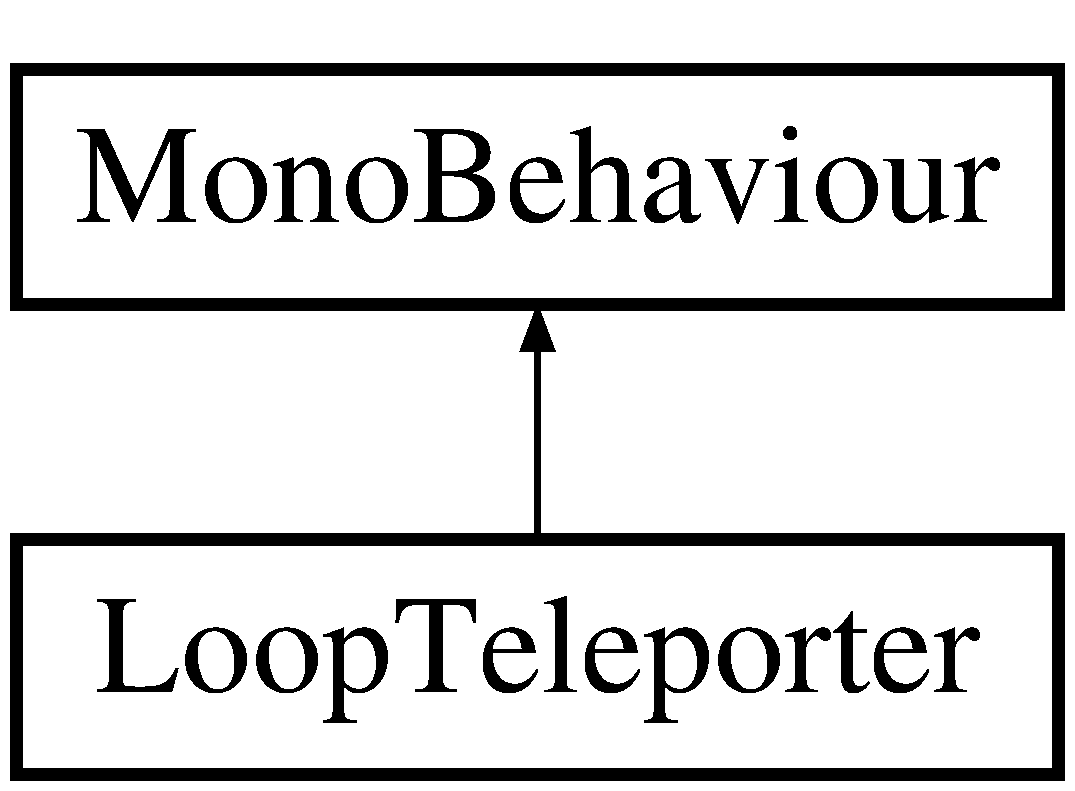
\includegraphics[height=2.000000cm]{class_loop_teleporter}
\end{center}
\end{figure}


The documentation for this class was generated from the following file\+:\begin{DoxyCompactItemize}
\item 
/\+Users/kwanholloway/git/5001\+Project/\+Game\+Project/\+Assets/\+Scripts/\+Game\+Logic/\hyperlink{_loop_teleporter_8cs}{Loop\+Teleporter.\+cs}\end{DoxyCompactItemize}

\hypertarget{class_message_panel}{}\section{Message\+Panel Class Reference}
\label{class_message_panel}\index{Message\+Panel@{Message\+Panel}}
Inheritance diagram for Message\+Panel\+:\begin{figure}[H]
\begin{center}
\leavevmode
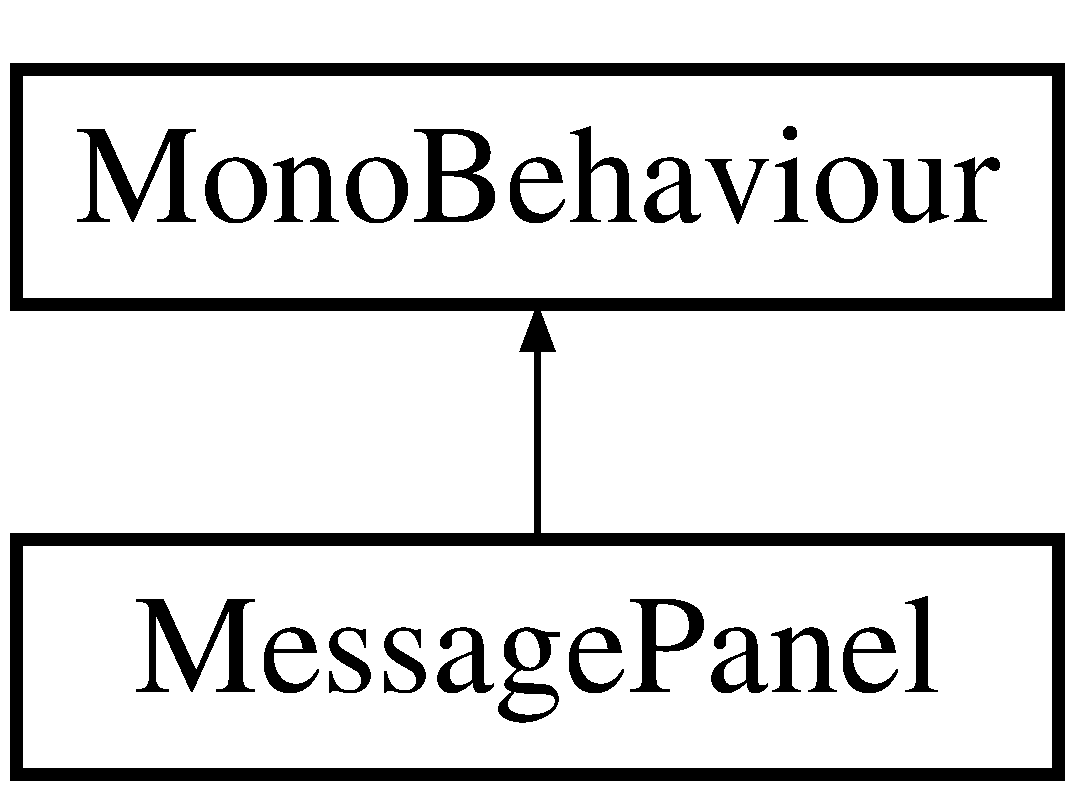
\includegraphics[height=2.000000cm]{class_message_panel}
\end{center}
\end{figure}
\subsection*{Public Attributes}
\begin{DoxyCompactItemize}
\item 
Text \hyperlink{class_message_panel_a8b8f813b410d2e40ff070399c7a964cb}{Word\+Display}
\item 
Game\+Object \hyperlink{class_message_panel_a7b8a8ec70900e2bfb62c29afb388f5ac}{button}
\end{DoxyCompactItemize}


\subsection{Member Data Documentation}
\mbox{\Hypertarget{class_message_panel_a7b8a8ec70900e2bfb62c29afb388f5ac}\label{class_message_panel_a7b8a8ec70900e2bfb62c29afb388f5ac}} 
\index{Message\+Panel@{Message\+Panel}!button@{button}}
\index{button@{button}!Message\+Panel@{Message\+Panel}}
\subsubsection{\texorpdfstring{button}{button}}
{\footnotesize\ttfamily Game\+Object Message\+Panel.\+button}

\mbox{\Hypertarget{class_message_panel_a8b8f813b410d2e40ff070399c7a964cb}\label{class_message_panel_a8b8f813b410d2e40ff070399c7a964cb}} 
\index{Message\+Panel@{Message\+Panel}!Word\+Display@{Word\+Display}}
\index{Word\+Display@{Word\+Display}!Message\+Panel@{Message\+Panel}}
\subsubsection{\texorpdfstring{Word\+Display}{WordDisplay}}
{\footnotesize\ttfamily Text Message\+Panel.\+Word\+Display}



The documentation for this class was generated from the following file\+:\begin{DoxyCompactItemize}
\item 
/\+Users/kwanholloway/git/5001\+Project/\+Game\+Project/\+Assets/\+Scripts/\+Game\+Logic/\hyperlink{_message_panel_8cs}{Message\+Panel.\+cs}\end{DoxyCompactItemize}

\hypertarget{class_moving_object}{}\section{Moving\+Object Class Reference}
\label{class_moving_object}\index{Moving\+Object@{Moving\+Object}}
Inheritance diagram for Moving\+Object\+:\begin{figure}[H]
\begin{center}
\leavevmode
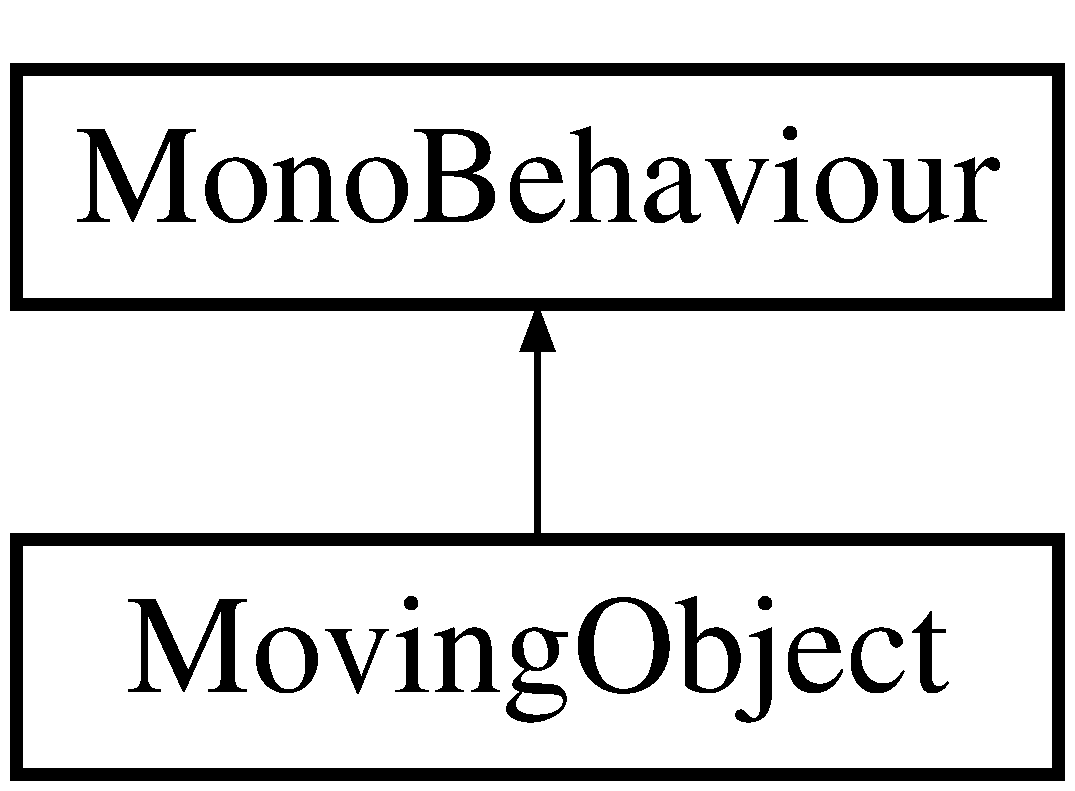
\includegraphics[height=2.000000cm]{class_moving_object}
\end{center}
\end{figure}
\subsection*{Public Attributes}
\begin{DoxyCompactItemize}
\item 
Game\+Object \hyperlink{class_moving_object_af4b69a184bdd5b7fdf9f7971fd4f0a33}{object\+To\+Move}
\item 
Transform \hyperlink{class_moving_object_a0e64d125d08a40852bfb66f95ed1ae18}{start\+Point}
\item 
Transform \hyperlink{class_moving_object_a4e00544427448aa5032d17a86ab29ea7}{end\+Point}
\item 
float \hyperlink{class_moving_object_a1b309484a50fd82bf6a370cd7186da36}{move\+Speed}
\end{DoxyCompactItemize}


\subsection{Member Data Documentation}
\mbox{\Hypertarget{class_moving_object_a4e00544427448aa5032d17a86ab29ea7}\label{class_moving_object_a4e00544427448aa5032d17a86ab29ea7}} 
\index{Moving\+Object@{Moving\+Object}!end\+Point@{end\+Point}}
\index{end\+Point@{end\+Point}!Moving\+Object@{Moving\+Object}}
\subsubsection{\texorpdfstring{end\+Point}{endPoint}}
{\footnotesize\ttfamily Transform Moving\+Object.\+end\+Point}

\mbox{\Hypertarget{class_moving_object_a1b309484a50fd82bf6a370cd7186da36}\label{class_moving_object_a1b309484a50fd82bf6a370cd7186da36}} 
\index{Moving\+Object@{Moving\+Object}!move\+Speed@{move\+Speed}}
\index{move\+Speed@{move\+Speed}!Moving\+Object@{Moving\+Object}}
\subsubsection{\texorpdfstring{move\+Speed}{moveSpeed}}
{\footnotesize\ttfamily float Moving\+Object.\+move\+Speed}

\mbox{\Hypertarget{class_moving_object_af4b69a184bdd5b7fdf9f7971fd4f0a33}\label{class_moving_object_af4b69a184bdd5b7fdf9f7971fd4f0a33}} 
\index{Moving\+Object@{Moving\+Object}!object\+To\+Move@{object\+To\+Move}}
\index{object\+To\+Move@{object\+To\+Move}!Moving\+Object@{Moving\+Object}}
\subsubsection{\texorpdfstring{object\+To\+Move}{objectToMove}}
{\footnotesize\ttfamily Game\+Object Moving\+Object.\+object\+To\+Move}

\mbox{\Hypertarget{class_moving_object_a0e64d125d08a40852bfb66f95ed1ae18}\label{class_moving_object_a0e64d125d08a40852bfb66f95ed1ae18}} 
\index{Moving\+Object@{Moving\+Object}!start\+Point@{start\+Point}}
\index{start\+Point@{start\+Point}!Moving\+Object@{Moving\+Object}}
\subsubsection{\texorpdfstring{start\+Point}{startPoint}}
{\footnotesize\ttfamily Transform Moving\+Object.\+start\+Point}



The documentation for this class was generated from the following file\+:\begin{DoxyCompactItemize}
\item 
/\+Users/kwanholloway/git/5001\+Project/\+Game\+Project/\+Assets/\+Scripts/\+Game\+Logic/\hyperlink{_moving_object_8cs}{Moving\+Object.\+cs}\end{DoxyCompactItemize}

\hypertarget{class_nested_for_desk_top_interaction}{}\section{Nested\+For\+Desk\+Top\+Interaction Class Reference}
\label{class_nested_for_desk_top_interaction}\index{Nested\+For\+Desk\+Top\+Interaction@{Nested\+For\+Desk\+Top\+Interaction}}
Inheritance diagram for Nested\+For\+Desk\+Top\+Interaction\+:\begin{figure}[H]
\begin{center}
\leavevmode
\includegraphics[height=2.000000cm]{class_nested_for_desk_top_interaction}
\end{center}
\end{figure}
\subsection*{Public Member Functions}
\begin{DoxyCompactItemize}
\item 
void \hyperlink{class_nested_for_desk_top_interaction_aa3cd864ad705ec50279c5ad57ba8d81f}{toggle\+Camera} ()
\end{DoxyCompactItemize}
\subsection*{Public Attributes}
\begin{DoxyCompactItemize}
\item 
Text \hyperlink{class_nested_for_desk_top_interaction_a1513d5ef78700420a7d21539bdacb9d3}{prompt}
\item 
Camera \hyperlink{class_nested_for_desk_top_interaction_a457df49c8287eacf8782725a46081520}{main\+Cam}
\item 
Camera \hyperlink{class_nested_for_desk_top_interaction_ab23a4eaa0c552fe591657fb7176b0dfb}{puzzle\+Cam}
\item 
bool \hyperlink{class_nested_for_desk_top_interaction_ab6810aa35ec82dd0f83652b1fd85ad30}{on\+Main\+Cam} = true
\end{DoxyCompactItemize}


\subsection{Member Function Documentation}
\mbox{\Hypertarget{class_nested_for_desk_top_interaction_aa3cd864ad705ec50279c5ad57ba8d81f}\label{class_nested_for_desk_top_interaction_aa3cd864ad705ec50279c5ad57ba8d81f}} 
\index{Nested\+For\+Desk\+Top\+Interaction@{Nested\+For\+Desk\+Top\+Interaction}!toggle\+Camera@{toggle\+Camera}}
\index{toggle\+Camera@{toggle\+Camera}!Nested\+For\+Desk\+Top\+Interaction@{Nested\+For\+Desk\+Top\+Interaction}}
\subsubsection{\texorpdfstring{toggle\+Camera()}{toggleCamera()}}
{\footnotesize\ttfamily void Nested\+For\+Desk\+Top\+Interaction.\+toggle\+Camera (\begin{DoxyParamCaption}{ }\end{DoxyParamCaption})}



\subsection{Member Data Documentation}
\mbox{\Hypertarget{class_nested_for_desk_top_interaction_a457df49c8287eacf8782725a46081520}\label{class_nested_for_desk_top_interaction_a457df49c8287eacf8782725a46081520}} 
\index{Nested\+For\+Desk\+Top\+Interaction@{Nested\+For\+Desk\+Top\+Interaction}!main\+Cam@{main\+Cam}}
\index{main\+Cam@{main\+Cam}!Nested\+For\+Desk\+Top\+Interaction@{Nested\+For\+Desk\+Top\+Interaction}}
\subsubsection{\texorpdfstring{main\+Cam}{mainCam}}
{\footnotesize\ttfamily Camera Nested\+For\+Desk\+Top\+Interaction.\+main\+Cam}

\mbox{\Hypertarget{class_nested_for_desk_top_interaction_ab6810aa35ec82dd0f83652b1fd85ad30}\label{class_nested_for_desk_top_interaction_ab6810aa35ec82dd0f83652b1fd85ad30}} 
\index{Nested\+For\+Desk\+Top\+Interaction@{Nested\+For\+Desk\+Top\+Interaction}!on\+Main\+Cam@{on\+Main\+Cam}}
\index{on\+Main\+Cam@{on\+Main\+Cam}!Nested\+For\+Desk\+Top\+Interaction@{Nested\+For\+Desk\+Top\+Interaction}}
\subsubsection{\texorpdfstring{on\+Main\+Cam}{onMainCam}}
{\footnotesize\ttfamily bool Nested\+For\+Desk\+Top\+Interaction.\+on\+Main\+Cam = true}

\mbox{\Hypertarget{class_nested_for_desk_top_interaction_a1513d5ef78700420a7d21539bdacb9d3}\label{class_nested_for_desk_top_interaction_a1513d5ef78700420a7d21539bdacb9d3}} 
\index{Nested\+For\+Desk\+Top\+Interaction@{Nested\+For\+Desk\+Top\+Interaction}!prompt@{prompt}}
\index{prompt@{prompt}!Nested\+For\+Desk\+Top\+Interaction@{Nested\+For\+Desk\+Top\+Interaction}}
\subsubsection{\texorpdfstring{prompt}{prompt}}
{\footnotesize\ttfamily Text Nested\+For\+Desk\+Top\+Interaction.\+prompt}

\mbox{\Hypertarget{class_nested_for_desk_top_interaction_ab23a4eaa0c552fe591657fb7176b0dfb}\label{class_nested_for_desk_top_interaction_ab23a4eaa0c552fe591657fb7176b0dfb}} 
\index{Nested\+For\+Desk\+Top\+Interaction@{Nested\+For\+Desk\+Top\+Interaction}!puzzle\+Cam@{puzzle\+Cam}}
\index{puzzle\+Cam@{puzzle\+Cam}!Nested\+For\+Desk\+Top\+Interaction@{Nested\+For\+Desk\+Top\+Interaction}}
\subsubsection{\texorpdfstring{puzzle\+Cam}{puzzleCam}}
{\footnotesize\ttfamily Camera Nested\+For\+Desk\+Top\+Interaction.\+puzzle\+Cam}



The documentation for this class was generated from the following file\+:\begin{DoxyCompactItemize}
\item 
/\+Users/kwanholloway/git/5001\+Project/\+Game\+Project/\+Assets/\+Scripts/\+Game\+Logic/\hyperlink{_nested_for_desk_top_interaction_8cs}{Nested\+For\+Desk\+Top\+Interaction.\+cs}\end{DoxyCompactItemize}

\hypertarget{class_nested_for_j_i_t}{}\section{Nested\+For\+J\+IT Class Reference}
\label{class_nested_for_j_i_t}\index{Nested\+For\+J\+IT@{Nested\+For\+J\+IT}}
Inheritance diagram for Nested\+For\+J\+IT\+:\begin{figure}[H]
\begin{center}
\leavevmode
\includegraphics[height=2.000000cm]{class_nested_for_j_i_t}
\end{center}
\end{figure}
\subsection*{Public Member Functions}
\begin{DoxyCompactItemize}
\item 
void \hyperlink{class_nested_for_j_i_t_a4d5794378db84bf4c5a8e47cb0fdf22e}{show\+Text\+One} ()
\item 
void \hyperlink{class_nested_for_j_i_t_a2947c4b7bdcc425be675bd988c283031}{show\+Text\+Two} ()
\item 
void \hyperlink{class_nested_for_j_i_t_aa2572d2149aef7acd4de9de1252e33f7}{show\+Text\+Three} ()
\item 
void \hyperlink{class_nested_for_j_i_t_ad9cf9f87e9f3664bf012e7f8306e3a4f}{show\+Text\+Four} ()
\end{DoxyCompactItemize}
\subsection*{Public Attributes}
\begin{DoxyCompactItemize}
\item 
Text \hyperlink{class_nested_for_j_i_t_ad3d5a4ec0034f914c533ba9da9614ce5}{help}
\item 
bool \hyperlink{class_nested_for_j_i_t_ad2b53657e8277ec61faf775924102a7e}{down} = false
\end{DoxyCompactItemize}


\subsection{Member Function Documentation}
\mbox{\Hypertarget{class_nested_for_j_i_t_ad9cf9f87e9f3664bf012e7f8306e3a4f}\label{class_nested_for_j_i_t_ad9cf9f87e9f3664bf012e7f8306e3a4f}} 
\index{Nested\+For\+J\+IT@{Nested\+For\+J\+IT}!show\+Text\+Four@{show\+Text\+Four}}
\index{show\+Text\+Four@{show\+Text\+Four}!Nested\+For\+J\+IT@{Nested\+For\+J\+IT}}
\subsubsection{\texorpdfstring{show\+Text\+Four()}{showTextFour()}}
{\footnotesize\ttfamily void Nested\+For\+J\+I\+T.\+show\+Text\+Four (\begin{DoxyParamCaption}{ }\end{DoxyParamCaption})}

\mbox{\Hypertarget{class_nested_for_j_i_t_a4d5794378db84bf4c5a8e47cb0fdf22e}\label{class_nested_for_j_i_t_a4d5794378db84bf4c5a8e47cb0fdf22e}} 
\index{Nested\+For\+J\+IT@{Nested\+For\+J\+IT}!show\+Text\+One@{show\+Text\+One}}
\index{show\+Text\+One@{show\+Text\+One}!Nested\+For\+J\+IT@{Nested\+For\+J\+IT}}
\subsubsection{\texorpdfstring{show\+Text\+One()}{showTextOne()}}
{\footnotesize\ttfamily void Nested\+For\+J\+I\+T.\+show\+Text\+One (\begin{DoxyParamCaption}{ }\end{DoxyParamCaption})}

\mbox{\Hypertarget{class_nested_for_j_i_t_aa2572d2149aef7acd4de9de1252e33f7}\label{class_nested_for_j_i_t_aa2572d2149aef7acd4de9de1252e33f7}} 
\index{Nested\+For\+J\+IT@{Nested\+For\+J\+IT}!show\+Text\+Three@{show\+Text\+Three}}
\index{show\+Text\+Three@{show\+Text\+Three}!Nested\+For\+J\+IT@{Nested\+For\+J\+IT}}
\subsubsection{\texorpdfstring{show\+Text\+Three()}{showTextThree()}}
{\footnotesize\ttfamily void Nested\+For\+J\+I\+T.\+show\+Text\+Three (\begin{DoxyParamCaption}{ }\end{DoxyParamCaption})}

\mbox{\Hypertarget{class_nested_for_j_i_t_a2947c4b7bdcc425be675bd988c283031}\label{class_nested_for_j_i_t_a2947c4b7bdcc425be675bd988c283031}} 
\index{Nested\+For\+J\+IT@{Nested\+For\+J\+IT}!show\+Text\+Two@{show\+Text\+Two}}
\index{show\+Text\+Two@{show\+Text\+Two}!Nested\+For\+J\+IT@{Nested\+For\+J\+IT}}
\subsubsection{\texorpdfstring{show\+Text\+Two()}{showTextTwo()}}
{\footnotesize\ttfamily void Nested\+For\+J\+I\+T.\+show\+Text\+Two (\begin{DoxyParamCaption}{ }\end{DoxyParamCaption})}



\subsection{Member Data Documentation}
\mbox{\Hypertarget{class_nested_for_j_i_t_ad2b53657e8277ec61faf775924102a7e}\label{class_nested_for_j_i_t_ad2b53657e8277ec61faf775924102a7e}} 
\index{Nested\+For\+J\+IT@{Nested\+For\+J\+IT}!down@{down}}
\index{down@{down}!Nested\+For\+J\+IT@{Nested\+For\+J\+IT}}
\subsubsection{\texorpdfstring{down}{down}}
{\footnotesize\ttfamily bool Nested\+For\+J\+I\+T.\+down = false}

\mbox{\Hypertarget{class_nested_for_j_i_t_ad3d5a4ec0034f914c533ba9da9614ce5}\label{class_nested_for_j_i_t_ad3d5a4ec0034f914c533ba9da9614ce5}} 
\index{Nested\+For\+J\+IT@{Nested\+For\+J\+IT}!help@{help}}
\index{help@{help}!Nested\+For\+J\+IT@{Nested\+For\+J\+IT}}
\subsubsection{\texorpdfstring{help}{help}}
{\footnotesize\ttfamily Text Nested\+For\+J\+I\+T.\+help}



The documentation for this class was generated from the following file\+:\begin{DoxyCompactItemize}
\item 
/\+Users/kwanholloway/git/5001\+Project/\+Game\+Project/\+Assets/\+Scripts/\+Z-\/\+N\+O\+T U\+S\+E\+D/\hyperlink{_nested_for_j_i_t_8cs}{Nested\+For\+J\+I\+T.\+cs}\end{DoxyCompactItemize}

\hypertarget{class_one_way_moving_object}{}\section{One\+Way\+Moving\+Object Class Reference}
\label{class_one_way_moving_object}\index{One\+Way\+Moving\+Object@{One\+Way\+Moving\+Object}}
Inheritance diagram for One\+Way\+Moving\+Object\+:\begin{figure}[H]
\begin{center}
\leavevmode
\includegraphics[height=2.000000cm]{class_one_way_moving_object}
\end{center}
\end{figure}
\subsection*{Public Member Functions}
\begin{DoxyCompactItemize}
\item 
bool \hyperlink{class_one_way_moving_object_a09d08513eaa584681898a1c13d33de1c}{is\+Finished\+Moving} ()
\end{DoxyCompactItemize}
\subsection*{Public Attributes}
\begin{DoxyCompactItemize}
\item 
Game\+Object \hyperlink{class_one_way_moving_object_a738199df4fd9102323b3031b91f27cee}{obj\+To\+Move}
\item 
Transform \hyperlink{class_one_way_moving_object_ada34abca5c152d343ca7ce4f8d526386}{end\+Point}
\item 
float \hyperlink{class_one_way_moving_object_a57d03a6a88136b9c0a2fb931d3753fbd}{move\+Speed}
\item 
Vector3 \hyperlink{class_one_way_moving_object_a3373e130216d4a6ef9f6ba38083aee8b}{initial\+Position}
\item 
bool \hyperlink{class_one_way_moving_object_aa188d5bd0f6dd799966acebc9088471f}{finished\+Moving}
\end{DoxyCompactItemize}


\subsection{Member Function Documentation}
\mbox{\Hypertarget{class_one_way_moving_object_a09d08513eaa584681898a1c13d33de1c}\label{class_one_way_moving_object_a09d08513eaa584681898a1c13d33de1c}} 
\index{One\+Way\+Moving\+Object@{One\+Way\+Moving\+Object}!is\+Finished\+Moving@{is\+Finished\+Moving}}
\index{is\+Finished\+Moving@{is\+Finished\+Moving}!One\+Way\+Moving\+Object@{One\+Way\+Moving\+Object}}
\subsubsection{\texorpdfstring{is\+Finished\+Moving()}{isFinishedMoving()}}
{\footnotesize\ttfamily bool One\+Way\+Moving\+Object.\+is\+Finished\+Moving (\begin{DoxyParamCaption}{ }\end{DoxyParamCaption})}



\subsection{Member Data Documentation}
\mbox{\Hypertarget{class_one_way_moving_object_ada34abca5c152d343ca7ce4f8d526386}\label{class_one_way_moving_object_ada34abca5c152d343ca7ce4f8d526386}} 
\index{One\+Way\+Moving\+Object@{One\+Way\+Moving\+Object}!end\+Point@{end\+Point}}
\index{end\+Point@{end\+Point}!One\+Way\+Moving\+Object@{One\+Way\+Moving\+Object}}
\subsubsection{\texorpdfstring{end\+Point}{endPoint}}
{\footnotesize\ttfamily Transform One\+Way\+Moving\+Object.\+end\+Point}

\mbox{\Hypertarget{class_one_way_moving_object_aa188d5bd0f6dd799966acebc9088471f}\label{class_one_way_moving_object_aa188d5bd0f6dd799966acebc9088471f}} 
\index{One\+Way\+Moving\+Object@{One\+Way\+Moving\+Object}!finished\+Moving@{finished\+Moving}}
\index{finished\+Moving@{finished\+Moving}!One\+Way\+Moving\+Object@{One\+Way\+Moving\+Object}}
\subsubsection{\texorpdfstring{finished\+Moving}{finishedMoving}}
{\footnotesize\ttfamily bool One\+Way\+Moving\+Object.\+finished\+Moving}

\mbox{\Hypertarget{class_one_way_moving_object_a3373e130216d4a6ef9f6ba38083aee8b}\label{class_one_way_moving_object_a3373e130216d4a6ef9f6ba38083aee8b}} 
\index{One\+Way\+Moving\+Object@{One\+Way\+Moving\+Object}!initial\+Position@{initial\+Position}}
\index{initial\+Position@{initial\+Position}!One\+Way\+Moving\+Object@{One\+Way\+Moving\+Object}}
\subsubsection{\texorpdfstring{initial\+Position}{initialPosition}}
{\footnotesize\ttfamily Vector3 One\+Way\+Moving\+Object.\+initial\+Position}

\mbox{\Hypertarget{class_one_way_moving_object_a57d03a6a88136b9c0a2fb931d3753fbd}\label{class_one_way_moving_object_a57d03a6a88136b9c0a2fb931d3753fbd}} 
\index{One\+Way\+Moving\+Object@{One\+Way\+Moving\+Object}!move\+Speed@{move\+Speed}}
\index{move\+Speed@{move\+Speed}!One\+Way\+Moving\+Object@{One\+Way\+Moving\+Object}}
\subsubsection{\texorpdfstring{move\+Speed}{moveSpeed}}
{\footnotesize\ttfamily float One\+Way\+Moving\+Object.\+move\+Speed}

\mbox{\Hypertarget{class_one_way_moving_object_a738199df4fd9102323b3031b91f27cee}\label{class_one_way_moving_object_a738199df4fd9102323b3031b91f27cee}} 
\index{One\+Way\+Moving\+Object@{One\+Way\+Moving\+Object}!obj\+To\+Move@{obj\+To\+Move}}
\index{obj\+To\+Move@{obj\+To\+Move}!One\+Way\+Moving\+Object@{One\+Way\+Moving\+Object}}
\subsubsection{\texorpdfstring{obj\+To\+Move}{objToMove}}
{\footnotesize\ttfamily Game\+Object One\+Way\+Moving\+Object.\+obj\+To\+Move}



The documentation for this class was generated from the following file\+:\begin{DoxyCompactItemize}
\item 
/\+Users/kwanholloway/git/5001\+Project/\+Game\+Project/\+Assets/\+Scripts/\+Game\+Logic/\hyperlink{_one_way_moving_object_8cs}{One\+Way\+Moving\+Object.\+cs}\end{DoxyCompactItemize}

\hypertarget{class_one_way_moving_object_trigger}{}\section{One\+Way\+Moving\+Object\+Trigger Class Reference}
\label{class_one_way_moving_object_trigger}\index{One\+Way\+Moving\+Object\+Trigger@{One\+Way\+Moving\+Object\+Trigger}}
Inheritance diagram for One\+Way\+Moving\+Object\+Trigger\+:\begin{figure}[H]
\begin{center}
\leavevmode
\includegraphics[height=2.000000cm]{class_one_way_moving_object_trigger}
\end{center}
\end{figure}
\subsection*{Public Member Functions}
\begin{DoxyCompactItemize}
\item 
void \hyperlink{class_one_way_moving_object_trigger_a5ca6243e428f0bf25078650bce538acf}{move\+Object\+One\+Way} ()
\begin{DoxyCompactList}\small\item\em Responsible for moving the object. \end{DoxyCompactList}\item 
void \hyperlink{class_one_way_moving_object_trigger_a4005f31ac588ca0362062a12061f1739}{reset\+Position} ()
\begin{DoxyCompactList}\small\item\em resets the position of the object \end{DoxyCompactList}\end{DoxyCompactItemize}
\subsection*{Public Attributes}
\begin{DoxyCompactItemize}
\item 
\hyperlink{class_player_movement}{Player\+Movement} \hyperlink{class_one_way_moving_object_trigger_a50456b25de1017bd53ae8950dff38148}{player}
\begin{DoxyCompactList}\small\item\em reference to the player \end{DoxyCompactList}\item 
\hyperlink{class_j_i_t_script}{J\+I\+T\+Script} \hyperlink{class_one_way_moving_object_trigger_a826ac8904700117919e40f3954901ba6}{trigger\+Collider}
\begin{DoxyCompactList}\small\item\em trigger for the object \end{DoxyCompactList}\item 
Game\+Object \hyperlink{class_one_way_moving_object_trigger_a06663ffd79fa0ce74d186b0795d6b01b}{obj\+To\+Move}
\begin{DoxyCompactList}\small\item\em object to be moved \end{DoxyCompactList}\item 
Transform \hyperlink{class_one_way_moving_object_trigger_adee5de068d168a1b99fcf1f7e479150b}{end\+Point}
\begin{DoxyCompactList}\small\item\em ending point \end{DoxyCompactList}\item 
float \hyperlink{class_one_way_moving_object_trigger_a6da43dfdc11bf6498791d5a38e40722c}{move\+Speed}
\begin{DoxyCompactList}\small\item\em how fast the object moves \end{DoxyCompactList}\item 
Vector3 \hyperlink{class_one_way_moving_object_trigger_a86013b9388d8c1e3a88fd0fd2e8c6176}{initial\+Position}
\begin{DoxyCompactList}\small\item\em initial pos of the object \end{DoxyCompactList}\end{DoxyCompactItemize}


\subsection{Detailed Description}
Manages objects that are designed to move toward a goal only once This script used a trigger to detect the player The object only moves if the player hits the trigger 

\subsection{Member Function Documentation}
\mbox{\Hypertarget{class_one_way_moving_object_trigger_a5ca6243e428f0bf25078650bce538acf}\label{class_one_way_moving_object_trigger_a5ca6243e428f0bf25078650bce538acf}} 
\index{One\+Way\+Moving\+Object\+Trigger@{One\+Way\+Moving\+Object\+Trigger}!move\+Object\+One\+Way@{move\+Object\+One\+Way}}
\index{move\+Object\+One\+Way@{move\+Object\+One\+Way}!One\+Way\+Moving\+Object\+Trigger@{One\+Way\+Moving\+Object\+Trigger}}
\subsubsection{\texorpdfstring{move\+Object\+One\+Way()}{moveObjectOneWay()}}
{\footnotesize\ttfamily void One\+Way\+Moving\+Object\+Trigger.\+move\+Object\+One\+Way (\begin{DoxyParamCaption}{ }\end{DoxyParamCaption})}



Responsible for moving the object. 

\mbox{\Hypertarget{class_one_way_moving_object_trigger_a4005f31ac588ca0362062a12061f1739}\label{class_one_way_moving_object_trigger_a4005f31ac588ca0362062a12061f1739}} 
\index{One\+Way\+Moving\+Object\+Trigger@{One\+Way\+Moving\+Object\+Trigger}!reset\+Position@{reset\+Position}}
\index{reset\+Position@{reset\+Position}!One\+Way\+Moving\+Object\+Trigger@{One\+Way\+Moving\+Object\+Trigger}}
\subsubsection{\texorpdfstring{reset\+Position()}{resetPosition()}}
{\footnotesize\ttfamily void One\+Way\+Moving\+Object\+Trigger.\+reset\+Position (\begin{DoxyParamCaption}{ }\end{DoxyParamCaption})}



resets the position of the object 



\subsection{Member Data Documentation}
\mbox{\Hypertarget{class_one_way_moving_object_trigger_adee5de068d168a1b99fcf1f7e479150b}\label{class_one_way_moving_object_trigger_adee5de068d168a1b99fcf1f7e479150b}} 
\index{One\+Way\+Moving\+Object\+Trigger@{One\+Way\+Moving\+Object\+Trigger}!end\+Point@{end\+Point}}
\index{end\+Point@{end\+Point}!One\+Way\+Moving\+Object\+Trigger@{One\+Way\+Moving\+Object\+Trigger}}
\subsubsection{\texorpdfstring{end\+Point}{endPoint}}
{\footnotesize\ttfamily Transform One\+Way\+Moving\+Object\+Trigger.\+end\+Point}



ending point 

\mbox{\Hypertarget{class_one_way_moving_object_trigger_a86013b9388d8c1e3a88fd0fd2e8c6176}\label{class_one_way_moving_object_trigger_a86013b9388d8c1e3a88fd0fd2e8c6176}} 
\index{One\+Way\+Moving\+Object\+Trigger@{One\+Way\+Moving\+Object\+Trigger}!initial\+Position@{initial\+Position}}
\index{initial\+Position@{initial\+Position}!One\+Way\+Moving\+Object\+Trigger@{One\+Way\+Moving\+Object\+Trigger}}
\subsubsection{\texorpdfstring{initial\+Position}{initialPosition}}
{\footnotesize\ttfamily Vector3 One\+Way\+Moving\+Object\+Trigger.\+initial\+Position}



initial pos of the object 

\mbox{\Hypertarget{class_one_way_moving_object_trigger_a6da43dfdc11bf6498791d5a38e40722c}\label{class_one_way_moving_object_trigger_a6da43dfdc11bf6498791d5a38e40722c}} 
\index{One\+Way\+Moving\+Object\+Trigger@{One\+Way\+Moving\+Object\+Trigger}!move\+Speed@{move\+Speed}}
\index{move\+Speed@{move\+Speed}!One\+Way\+Moving\+Object\+Trigger@{One\+Way\+Moving\+Object\+Trigger}}
\subsubsection{\texorpdfstring{move\+Speed}{moveSpeed}}
{\footnotesize\ttfamily float One\+Way\+Moving\+Object\+Trigger.\+move\+Speed}



how fast the object moves 

\mbox{\Hypertarget{class_one_way_moving_object_trigger_a06663ffd79fa0ce74d186b0795d6b01b}\label{class_one_way_moving_object_trigger_a06663ffd79fa0ce74d186b0795d6b01b}} 
\index{One\+Way\+Moving\+Object\+Trigger@{One\+Way\+Moving\+Object\+Trigger}!obj\+To\+Move@{obj\+To\+Move}}
\index{obj\+To\+Move@{obj\+To\+Move}!One\+Way\+Moving\+Object\+Trigger@{One\+Way\+Moving\+Object\+Trigger}}
\subsubsection{\texorpdfstring{obj\+To\+Move}{objToMove}}
{\footnotesize\ttfamily Game\+Object One\+Way\+Moving\+Object\+Trigger.\+obj\+To\+Move}



object to be moved 

\mbox{\Hypertarget{class_one_way_moving_object_trigger_a50456b25de1017bd53ae8950dff38148}\label{class_one_way_moving_object_trigger_a50456b25de1017bd53ae8950dff38148}} 
\index{One\+Way\+Moving\+Object\+Trigger@{One\+Way\+Moving\+Object\+Trigger}!player@{player}}
\index{player@{player}!One\+Way\+Moving\+Object\+Trigger@{One\+Way\+Moving\+Object\+Trigger}}
\subsubsection{\texorpdfstring{player}{player}}
{\footnotesize\ttfamily \hyperlink{class_player_movement}{Player\+Movement} One\+Way\+Moving\+Object\+Trigger.\+player}



reference to the player 

\mbox{\Hypertarget{class_one_way_moving_object_trigger_a826ac8904700117919e40f3954901ba6}\label{class_one_way_moving_object_trigger_a826ac8904700117919e40f3954901ba6}} 
\index{One\+Way\+Moving\+Object\+Trigger@{One\+Way\+Moving\+Object\+Trigger}!trigger\+Collider@{trigger\+Collider}}
\index{trigger\+Collider@{trigger\+Collider}!One\+Way\+Moving\+Object\+Trigger@{One\+Way\+Moving\+Object\+Trigger}}
\subsubsection{\texorpdfstring{trigger\+Collider}{triggerCollider}}
{\footnotesize\ttfamily \hyperlink{class_j_i_t_script}{J\+I\+T\+Script} One\+Way\+Moving\+Object\+Trigger.\+trigger\+Collider}



trigger for the object 



The documentation for this class was generated from the following file\+:\begin{DoxyCompactItemize}
\item 
/\+Users/kwanholloway/git/5001\+Project/\+Game\+Project/\+Assets/\+Scripts/\+Game\+Logic/\hyperlink{_one_way_moving_object_trigger_8cs}{One\+Way\+Moving\+Object\+Trigger.\+cs}\end{DoxyCompactItemize}

\hypertarget{class_p2}{}\section{P2 Class Reference}
\label{class_p2}\index{P2@{P2}}
Inheritance diagram for P2\+:\begin{figure}[H]
\begin{center}
\leavevmode
\includegraphics[height=2.000000cm]{class_p2}
\end{center}
\end{figure}
\subsection*{Public Member Functions}
\begin{DoxyCompactItemize}
\item 
void \hyperlink{class_p2_ab7d360c4594f6a3a449a8bf493f9cf15}{show\+Text\+One} ()
\item 
void \hyperlink{class_p2_a152ef7f6e9de4265caf63cf2a1f70822}{show\+Text\+Two} ()
\item 
void \hyperlink{class_p2_a780ca00a71e17fbe6e5047bdb11c90a4}{show\+Text\+Three} ()
\end{DoxyCompactItemize}
\subsection*{Public Attributes}
\begin{DoxyCompactItemize}
\item 
Text \hyperlink{class_p2_a2a27095e4b32343150d613a13fa0408a}{help}
\item 
bool \hyperlink{class_p2_a78207b72f4528ec324966d7aaa3f8dc9}{down} = false
\end{DoxyCompactItemize}


\subsection{Member Function Documentation}
\mbox{\Hypertarget{class_p2_ab7d360c4594f6a3a449a8bf493f9cf15}\label{class_p2_ab7d360c4594f6a3a449a8bf493f9cf15}} 
\index{P2@{P2}!show\+Text\+One@{show\+Text\+One}}
\index{show\+Text\+One@{show\+Text\+One}!P2@{P2}}
\subsubsection{\texorpdfstring{show\+Text\+One()}{showTextOne()}}
{\footnotesize\ttfamily void P2.\+show\+Text\+One (\begin{DoxyParamCaption}{ }\end{DoxyParamCaption})}

\mbox{\Hypertarget{class_p2_a780ca00a71e17fbe6e5047bdb11c90a4}\label{class_p2_a780ca00a71e17fbe6e5047bdb11c90a4}} 
\index{P2@{P2}!show\+Text\+Three@{show\+Text\+Three}}
\index{show\+Text\+Three@{show\+Text\+Three}!P2@{P2}}
\subsubsection{\texorpdfstring{show\+Text\+Three()}{showTextThree()}}
{\footnotesize\ttfamily void P2.\+show\+Text\+Three (\begin{DoxyParamCaption}{ }\end{DoxyParamCaption})}

\mbox{\Hypertarget{class_p2_a152ef7f6e9de4265caf63cf2a1f70822}\label{class_p2_a152ef7f6e9de4265caf63cf2a1f70822}} 
\index{P2@{P2}!show\+Text\+Two@{show\+Text\+Two}}
\index{show\+Text\+Two@{show\+Text\+Two}!P2@{P2}}
\subsubsection{\texorpdfstring{show\+Text\+Two()}{showTextTwo()}}
{\footnotesize\ttfamily void P2.\+show\+Text\+Two (\begin{DoxyParamCaption}{ }\end{DoxyParamCaption})}



\subsection{Member Data Documentation}
\mbox{\Hypertarget{class_p2_a78207b72f4528ec324966d7aaa3f8dc9}\label{class_p2_a78207b72f4528ec324966d7aaa3f8dc9}} 
\index{P2@{P2}!down@{down}}
\index{down@{down}!P2@{P2}}
\subsubsection{\texorpdfstring{down}{down}}
{\footnotesize\ttfamily bool P2.\+down = false}

\mbox{\Hypertarget{class_p2_a2a27095e4b32343150d613a13fa0408a}\label{class_p2_a2a27095e4b32343150d613a13fa0408a}} 
\index{P2@{P2}!help@{help}}
\index{help@{help}!P2@{P2}}
\subsubsection{\texorpdfstring{help}{help}}
{\footnotesize\ttfamily Text P2.\+help}



The documentation for this class was generated from the following file\+:\begin{DoxyCompactItemize}
\item 
/\+Users/kwanholloway/git/5001\+Project/\+Game\+Project/\+Assets/\+Scripts/\+Z-\/\+N\+O\+T U\+S\+E\+D/\hyperlink{_p2_8cs}{P2.\+cs}\end{DoxyCompactItemize}

\hypertarget{class_pause_menu}{}\section{Pause\+Menu Class Reference}
\label{class_pause_menu}\index{Pause\+Menu@{Pause\+Menu}}
Inheritance diagram for Pause\+Menu\+:\begin{figure}[H]
\begin{center}
\leavevmode
\includegraphics[height=2.000000cm]{class_pause_menu}
\end{center}
\end{figure}


The documentation for this class was generated from the following file\+:\begin{DoxyCompactItemize}
\item 
/\+Users/kwanholloway/git/5001\+Project/\+Game\+Project/\+Assets/\+Scripts/\+Game\+Logic/\hyperlink{_pause_menu_8cs}{Pause\+Menu.\+cs}\end{DoxyCompactItemize}

\hypertarget{classplace_scientists}{}\section{place\+Scientists Class Reference}
\label{classplace_scientists}\index{place\+Scientists@{place\+Scientists}}
Inheritance diagram for place\+Scientists\+:\begin{figure}[H]
\begin{center}
\leavevmode
\includegraphics[height=2.000000cm]{classplace_scientists}
\end{center}
\end{figure}
\subsection*{Public Attributes}
\begin{DoxyCompactItemize}
\item 
Game\+Object \hyperlink{classplace_scientists_a5ced1e88492dd766534202679f8e0fd4}{loop\+Scientists}
\end{DoxyCompactItemize}


\subsection{Member Data Documentation}
\mbox{\Hypertarget{classplace_scientists_a5ced1e88492dd766534202679f8e0fd4}\label{classplace_scientists_a5ced1e88492dd766534202679f8e0fd4}} 
\index{place\+Scientists@{place\+Scientists}!loop\+Scientists@{loop\+Scientists}}
\index{loop\+Scientists@{loop\+Scientists}!place\+Scientists@{place\+Scientists}}
\subsubsection{\texorpdfstring{loop\+Scientists}{loopScientists}}
{\footnotesize\ttfamily Game\+Object place\+Scientists.\+loop\+Scientists}



The documentation for this class was generated from the following file\+:\begin{DoxyCompactItemize}
\item 
/\+Users/kwanholloway/git/5001\+Project/\+Game\+Project/\+Assets/\+Scripts/\+Game\+Logic/\hyperlink{place_scientists_8cs}{place\+Scientists.\+cs}\end{DoxyCompactItemize}

\hypertarget{class_platform_access_controller}{}\section{Platform\+Access\+Controller Class Reference}
\label{class_platform_access_controller}\index{Platform\+Access\+Controller@{Platform\+Access\+Controller}}
Inheritance diagram for Platform\+Access\+Controller\+:\begin{figure}[H]
\begin{center}
\leavevmode
\includegraphics[height=2.000000cm]{class_platform_access_controller}
\end{center}
\end{figure}
\subsection*{Public Member Functions}
\begin{DoxyCompactItemize}
\item 
void \hyperlink{class_platform_access_controller_a3999dc4cf501e3092bf06662e215afaf}{Set\+Visible\+And\+Active} ()
\item 
void \hyperlink{class_platform_access_controller_adae7a500e267262f6262b9997fb7e9d4}{Set\+Invisible\+And\+Inactive} ()
\end{DoxyCompactItemize}
\subsection*{Public Attributes}
\begin{DoxyCompactItemize}
\item 
bool \hyperlink{class_platform_access_controller_ae61d142d689e9436ffcdd42ae258b74b}{is\+Visible}
\item 
Box\+Collider2D \hyperlink{class_platform_access_controller_a7e71633a42a42bd944656b6b31da7018}{b\+Col}
\item 
Sprite\+Renderer \hyperlink{class_platform_access_controller_a148223f08e156ce2c3cbf9b87feb83d2}{spr}
\item 
Sprite\+Renderer \hyperlink{class_platform_access_controller_a96b290b37dd60e9c78015b86c94ffbe7}{index\+Num\+Spr}
\end{DoxyCompactItemize}


\subsection{Member Function Documentation}
\mbox{\Hypertarget{class_platform_access_controller_adae7a500e267262f6262b9997fb7e9d4}\label{class_platform_access_controller_adae7a500e267262f6262b9997fb7e9d4}} 
\index{Platform\+Access\+Controller@{Platform\+Access\+Controller}!Set\+Invisible\+And\+Inactive@{Set\+Invisible\+And\+Inactive}}
\index{Set\+Invisible\+And\+Inactive@{Set\+Invisible\+And\+Inactive}!Platform\+Access\+Controller@{Platform\+Access\+Controller}}
\subsubsection{\texorpdfstring{Set\+Invisible\+And\+Inactive()}{SetInvisibleAndInactive()}}
{\footnotesize\ttfamily void Platform\+Access\+Controller.\+Set\+Invisible\+And\+Inactive (\begin{DoxyParamCaption}{ }\end{DoxyParamCaption})}

\mbox{\Hypertarget{class_platform_access_controller_a3999dc4cf501e3092bf06662e215afaf}\label{class_platform_access_controller_a3999dc4cf501e3092bf06662e215afaf}} 
\index{Platform\+Access\+Controller@{Platform\+Access\+Controller}!Set\+Visible\+And\+Active@{Set\+Visible\+And\+Active}}
\index{Set\+Visible\+And\+Active@{Set\+Visible\+And\+Active}!Platform\+Access\+Controller@{Platform\+Access\+Controller}}
\subsubsection{\texorpdfstring{Set\+Visible\+And\+Active()}{SetVisibleAndActive()}}
{\footnotesize\ttfamily void Platform\+Access\+Controller.\+Set\+Visible\+And\+Active (\begin{DoxyParamCaption}{ }\end{DoxyParamCaption})}



\subsection{Member Data Documentation}
\mbox{\Hypertarget{class_platform_access_controller_a7e71633a42a42bd944656b6b31da7018}\label{class_platform_access_controller_a7e71633a42a42bd944656b6b31da7018}} 
\index{Platform\+Access\+Controller@{Platform\+Access\+Controller}!b\+Col@{b\+Col}}
\index{b\+Col@{b\+Col}!Platform\+Access\+Controller@{Platform\+Access\+Controller}}
\subsubsection{\texorpdfstring{b\+Col}{bCol}}
{\footnotesize\ttfamily Box\+Collider2D Platform\+Access\+Controller.\+b\+Col}

\mbox{\Hypertarget{class_platform_access_controller_a96b290b37dd60e9c78015b86c94ffbe7}\label{class_platform_access_controller_a96b290b37dd60e9c78015b86c94ffbe7}} 
\index{Platform\+Access\+Controller@{Platform\+Access\+Controller}!index\+Num\+Spr@{index\+Num\+Spr}}
\index{index\+Num\+Spr@{index\+Num\+Spr}!Platform\+Access\+Controller@{Platform\+Access\+Controller}}
\subsubsection{\texorpdfstring{index\+Num\+Spr}{indexNumSpr}}
{\footnotesize\ttfamily Sprite\+Renderer Platform\+Access\+Controller.\+index\+Num\+Spr}

\mbox{\Hypertarget{class_platform_access_controller_ae61d142d689e9436ffcdd42ae258b74b}\label{class_platform_access_controller_ae61d142d689e9436ffcdd42ae258b74b}} 
\index{Platform\+Access\+Controller@{Platform\+Access\+Controller}!is\+Visible@{is\+Visible}}
\index{is\+Visible@{is\+Visible}!Platform\+Access\+Controller@{Platform\+Access\+Controller}}
\subsubsection{\texorpdfstring{is\+Visible}{isVisible}}
{\footnotesize\ttfamily bool Platform\+Access\+Controller.\+is\+Visible}

\mbox{\Hypertarget{class_platform_access_controller_a148223f08e156ce2c3cbf9b87feb83d2}\label{class_platform_access_controller_a148223f08e156ce2c3cbf9b87feb83d2}} 
\index{Platform\+Access\+Controller@{Platform\+Access\+Controller}!spr@{spr}}
\index{spr@{spr}!Platform\+Access\+Controller@{Platform\+Access\+Controller}}
\subsubsection{\texorpdfstring{spr}{spr}}
{\footnotesize\ttfamily Sprite\+Renderer Platform\+Access\+Controller.\+spr}



The documentation for this class was generated from the following file\+:\begin{DoxyCompactItemize}
\item 
/\+Users/kwanholloway/git/5001\+Project/\+Game\+Project/\+Assets/\+Scripts/\+Puzzle\+Logic/\+Array\+Access\+Puzzle/\hyperlink{_platform_access_controller_8cs}{Platform\+Access\+Controller.\+cs}\end{DoxyCompactItemize}

\hypertarget{class_player_movement}{}\section{Player\+Movement Class Reference}
\label{class_player_movement}\index{Player\+Movement@{Player\+Movement}}
Inheritance diagram for Player\+Movement\+:\begin{figure}[H]
\begin{center}
\leavevmode
\includegraphics[height=2.000000cm]{class_player_movement}
\end{center}
\end{figure}
\subsection*{Public Member Functions}
\begin{DoxyCompactItemize}
\item 
void \hyperlink{class_player_movement_a4801b0f4bea995d557faf3e0cf004b8b}{zoom\+Out} ()
\item 
void \hyperlink{class_player_movement_a86dee8b90e483c36b7190c80a53a4163}{zoom\+In} ()
\item 
void \hyperlink{class_player_movement_a53e0613db4bf57eb5edc2b9dacd7bfe5}{set\+Cam\+Size} (float new\+Cam\+Size)
\item 
void \hyperlink{class_player_movement_abd415fe1fd1e33f5fe5c28fa9ad97399}{go\+To\+Arr\+Platforms} ()
\end{DoxyCompactItemize}
\subsection*{Public Attributes}
\begin{DoxyCompactItemize}
\item 
float \hyperlink{class_player_movement_a93207dc2742fe0f0b651a54d610b14aa}{move\+Speed}
\item 
float \hyperlink{class_player_movement_a0b04326b12b370063895e93d1a20655d}{jump\+Speed}
\item 
bool \hyperlink{class_player_movement_a27276d8e80bcd5acbb70354b06d66841}{is\+Grounded}
\item 
bool \hyperlink{class_player_movement_a1a59782fc52356398194e29255f1a0ae}{is\+Jumping}
\item 
bool \hyperlink{class_player_movement_a9be62b9ccfa0da0b71b5247df817fe4b}{left\+Facing} = false
\item 
bool \hyperlink{class_player_movement_a93c85b6422113049146e1d40b215a8e2}{can\+Double\+Jump} = false
\item 
bool \hyperlink{class_player_movement_acddd245968579989670e4c0953ae2746}{can\+Speed\+Up}
\item 
Game\+Object \hyperlink{class_player_movement_a97e6c77c213a7631791776290199d532}{bomb}
\item 
\hyperlink{classbomb_logic}{bomb\+Logic} \hyperlink{class_player_movement_a5ea646039fd085e5c19acef918f24a21}{timer}
\item 
float \hyperlink{class_player_movement_ae6959aebc17336198f7eb270f21e2195}{start\+Time}
\item 
Transform \hyperlink{class_player_movement_a4c733d8e1fcc9ffd7223ac3182b380f5}{ground\+Check}
\item 
float \hyperlink{class_player_movement_a14516da52e9f1e37eea97c98afed9ff3}{ground\+Check\+Radius}
\item 
Layer\+Mask \hyperlink{class_player_movement_a04b4dc5a83828e9fefcfe8acbf5de276}{what\+Is\+Ground}
\item 
bool \hyperlink{class_player_movement_ae0fb74ddab994fb7627c7561629a8982}{zoom} = false
\item 
Camera \hyperlink{class_player_movement_a345feead60bc04aeb3bf54f198823097}{cam}
\item 
\hyperlink{class_global_controller}{Global\+Controller} \hyperlink{class_player_movement_adb2c84510e5bf27967dcff5bdfdf80d4}{game\+Manager}
\item 
\hyperlink{class_respawn_controller}{Respawn\+Controller} \hyperlink{class_player_movement_a9669ec66c625ff5409f8fb6be21fef12}{respawn\+Manager}
\end{DoxyCompactItemize}


\subsection{Member Function Documentation}
\mbox{\Hypertarget{class_player_movement_abd415fe1fd1e33f5fe5c28fa9ad97399}\label{class_player_movement_abd415fe1fd1e33f5fe5c28fa9ad97399}} 
\index{Player\+Movement@{Player\+Movement}!go\+To\+Arr\+Platforms@{go\+To\+Arr\+Platforms}}
\index{go\+To\+Arr\+Platforms@{go\+To\+Arr\+Platforms}!Player\+Movement@{Player\+Movement}}
\subsubsection{\texorpdfstring{go\+To\+Arr\+Platforms()}{goToArrPlatforms()}}
{\footnotesize\ttfamily void Player\+Movement.\+go\+To\+Arr\+Platforms (\begin{DoxyParamCaption}{ }\end{DoxyParamCaption})}

\mbox{\Hypertarget{class_player_movement_a53e0613db4bf57eb5edc2b9dacd7bfe5}\label{class_player_movement_a53e0613db4bf57eb5edc2b9dacd7bfe5}} 
\index{Player\+Movement@{Player\+Movement}!set\+Cam\+Size@{set\+Cam\+Size}}
\index{set\+Cam\+Size@{set\+Cam\+Size}!Player\+Movement@{Player\+Movement}}
\subsubsection{\texorpdfstring{set\+Cam\+Size()}{setCamSize()}}
{\footnotesize\ttfamily void Player\+Movement.\+set\+Cam\+Size (\begin{DoxyParamCaption}\item[{float}]{new\+Cam\+Size }\end{DoxyParamCaption})}

\mbox{\Hypertarget{class_player_movement_a86dee8b90e483c36b7190c80a53a4163}\label{class_player_movement_a86dee8b90e483c36b7190c80a53a4163}} 
\index{Player\+Movement@{Player\+Movement}!zoom\+In@{zoom\+In}}
\index{zoom\+In@{zoom\+In}!Player\+Movement@{Player\+Movement}}
\subsubsection{\texorpdfstring{zoom\+In()}{zoomIn()}}
{\footnotesize\ttfamily void Player\+Movement.\+zoom\+In (\begin{DoxyParamCaption}{ }\end{DoxyParamCaption})}

\mbox{\Hypertarget{class_player_movement_a4801b0f4bea995d557faf3e0cf004b8b}\label{class_player_movement_a4801b0f4bea995d557faf3e0cf004b8b}} 
\index{Player\+Movement@{Player\+Movement}!zoom\+Out@{zoom\+Out}}
\index{zoom\+Out@{zoom\+Out}!Player\+Movement@{Player\+Movement}}
\subsubsection{\texorpdfstring{zoom\+Out()}{zoomOut()}}
{\footnotesize\ttfamily void Player\+Movement.\+zoom\+Out (\begin{DoxyParamCaption}{ }\end{DoxyParamCaption})}



\subsection{Member Data Documentation}
\mbox{\Hypertarget{class_player_movement_a97e6c77c213a7631791776290199d532}\label{class_player_movement_a97e6c77c213a7631791776290199d532}} 
\index{Player\+Movement@{Player\+Movement}!bomb@{bomb}}
\index{bomb@{bomb}!Player\+Movement@{Player\+Movement}}
\subsubsection{\texorpdfstring{bomb}{bomb}}
{\footnotesize\ttfamily Game\+Object Player\+Movement.\+bomb}

\mbox{\Hypertarget{class_player_movement_a345feead60bc04aeb3bf54f198823097}\label{class_player_movement_a345feead60bc04aeb3bf54f198823097}} 
\index{Player\+Movement@{Player\+Movement}!cam@{cam}}
\index{cam@{cam}!Player\+Movement@{Player\+Movement}}
\subsubsection{\texorpdfstring{cam}{cam}}
{\footnotesize\ttfamily Camera Player\+Movement.\+cam}

\mbox{\Hypertarget{class_player_movement_a93c85b6422113049146e1d40b215a8e2}\label{class_player_movement_a93c85b6422113049146e1d40b215a8e2}} 
\index{Player\+Movement@{Player\+Movement}!can\+Double\+Jump@{can\+Double\+Jump}}
\index{can\+Double\+Jump@{can\+Double\+Jump}!Player\+Movement@{Player\+Movement}}
\subsubsection{\texorpdfstring{can\+Double\+Jump}{canDoubleJump}}
{\footnotesize\ttfamily bool Player\+Movement.\+can\+Double\+Jump = false}

\mbox{\Hypertarget{class_player_movement_acddd245968579989670e4c0953ae2746}\label{class_player_movement_acddd245968579989670e4c0953ae2746}} 
\index{Player\+Movement@{Player\+Movement}!can\+Speed\+Up@{can\+Speed\+Up}}
\index{can\+Speed\+Up@{can\+Speed\+Up}!Player\+Movement@{Player\+Movement}}
\subsubsection{\texorpdfstring{can\+Speed\+Up}{canSpeedUp}}
{\footnotesize\ttfamily bool Player\+Movement.\+can\+Speed\+Up}

\mbox{\Hypertarget{class_player_movement_adb2c84510e5bf27967dcff5bdfdf80d4}\label{class_player_movement_adb2c84510e5bf27967dcff5bdfdf80d4}} 
\index{Player\+Movement@{Player\+Movement}!game\+Manager@{game\+Manager}}
\index{game\+Manager@{game\+Manager}!Player\+Movement@{Player\+Movement}}
\subsubsection{\texorpdfstring{game\+Manager}{gameManager}}
{\footnotesize\ttfamily \hyperlink{class_global_controller}{Global\+Controller} Player\+Movement.\+game\+Manager}

\mbox{\Hypertarget{class_player_movement_a4c733d8e1fcc9ffd7223ac3182b380f5}\label{class_player_movement_a4c733d8e1fcc9ffd7223ac3182b380f5}} 
\index{Player\+Movement@{Player\+Movement}!ground\+Check@{ground\+Check}}
\index{ground\+Check@{ground\+Check}!Player\+Movement@{Player\+Movement}}
\subsubsection{\texorpdfstring{ground\+Check}{groundCheck}}
{\footnotesize\ttfamily Transform Player\+Movement.\+ground\+Check}

\mbox{\Hypertarget{class_player_movement_a14516da52e9f1e37eea97c98afed9ff3}\label{class_player_movement_a14516da52e9f1e37eea97c98afed9ff3}} 
\index{Player\+Movement@{Player\+Movement}!ground\+Check\+Radius@{ground\+Check\+Radius}}
\index{ground\+Check\+Radius@{ground\+Check\+Radius}!Player\+Movement@{Player\+Movement}}
\subsubsection{\texorpdfstring{ground\+Check\+Radius}{groundCheckRadius}}
{\footnotesize\ttfamily float Player\+Movement.\+ground\+Check\+Radius}

\mbox{\Hypertarget{class_player_movement_a27276d8e80bcd5acbb70354b06d66841}\label{class_player_movement_a27276d8e80bcd5acbb70354b06d66841}} 
\index{Player\+Movement@{Player\+Movement}!is\+Grounded@{is\+Grounded}}
\index{is\+Grounded@{is\+Grounded}!Player\+Movement@{Player\+Movement}}
\subsubsection{\texorpdfstring{is\+Grounded}{isGrounded}}
{\footnotesize\ttfamily bool Player\+Movement.\+is\+Grounded}

\mbox{\Hypertarget{class_player_movement_a1a59782fc52356398194e29255f1a0ae}\label{class_player_movement_a1a59782fc52356398194e29255f1a0ae}} 
\index{Player\+Movement@{Player\+Movement}!is\+Jumping@{is\+Jumping}}
\index{is\+Jumping@{is\+Jumping}!Player\+Movement@{Player\+Movement}}
\subsubsection{\texorpdfstring{is\+Jumping}{isJumping}}
{\footnotesize\ttfamily bool Player\+Movement.\+is\+Jumping}

\mbox{\Hypertarget{class_player_movement_a0b04326b12b370063895e93d1a20655d}\label{class_player_movement_a0b04326b12b370063895e93d1a20655d}} 
\index{Player\+Movement@{Player\+Movement}!jump\+Speed@{jump\+Speed}}
\index{jump\+Speed@{jump\+Speed}!Player\+Movement@{Player\+Movement}}
\subsubsection{\texorpdfstring{jump\+Speed}{jumpSpeed}}
{\footnotesize\ttfamily float Player\+Movement.\+jump\+Speed}

\mbox{\Hypertarget{class_player_movement_a9be62b9ccfa0da0b71b5247df817fe4b}\label{class_player_movement_a9be62b9ccfa0da0b71b5247df817fe4b}} 
\index{Player\+Movement@{Player\+Movement}!left\+Facing@{left\+Facing}}
\index{left\+Facing@{left\+Facing}!Player\+Movement@{Player\+Movement}}
\subsubsection{\texorpdfstring{left\+Facing}{leftFacing}}
{\footnotesize\ttfamily bool Player\+Movement.\+left\+Facing = false}

\mbox{\Hypertarget{class_player_movement_a93207dc2742fe0f0b651a54d610b14aa}\label{class_player_movement_a93207dc2742fe0f0b651a54d610b14aa}} 
\index{Player\+Movement@{Player\+Movement}!move\+Speed@{move\+Speed}}
\index{move\+Speed@{move\+Speed}!Player\+Movement@{Player\+Movement}}
\subsubsection{\texorpdfstring{move\+Speed}{moveSpeed}}
{\footnotesize\ttfamily float Player\+Movement.\+move\+Speed}

\mbox{\Hypertarget{class_player_movement_a9669ec66c625ff5409f8fb6be21fef12}\label{class_player_movement_a9669ec66c625ff5409f8fb6be21fef12}} 
\index{Player\+Movement@{Player\+Movement}!respawn\+Manager@{respawn\+Manager}}
\index{respawn\+Manager@{respawn\+Manager}!Player\+Movement@{Player\+Movement}}
\subsubsection{\texorpdfstring{respawn\+Manager}{respawnManager}}
{\footnotesize\ttfamily \hyperlink{class_respawn_controller}{Respawn\+Controller} Player\+Movement.\+respawn\+Manager}

\mbox{\Hypertarget{class_player_movement_ae6959aebc17336198f7eb270f21e2195}\label{class_player_movement_ae6959aebc17336198f7eb270f21e2195}} 
\index{Player\+Movement@{Player\+Movement}!start\+Time@{start\+Time}}
\index{start\+Time@{start\+Time}!Player\+Movement@{Player\+Movement}}
\subsubsection{\texorpdfstring{start\+Time}{startTime}}
{\footnotesize\ttfamily float Player\+Movement.\+start\+Time}

\mbox{\Hypertarget{class_player_movement_a5ea646039fd085e5c19acef918f24a21}\label{class_player_movement_a5ea646039fd085e5c19acef918f24a21}} 
\index{Player\+Movement@{Player\+Movement}!timer@{timer}}
\index{timer@{timer}!Player\+Movement@{Player\+Movement}}
\subsubsection{\texorpdfstring{timer}{timer}}
{\footnotesize\ttfamily \hyperlink{classbomb_logic}{bomb\+Logic} Player\+Movement.\+timer}

\mbox{\Hypertarget{class_player_movement_a04b4dc5a83828e9fefcfe8acbf5de276}\label{class_player_movement_a04b4dc5a83828e9fefcfe8acbf5de276}} 
\index{Player\+Movement@{Player\+Movement}!what\+Is\+Ground@{what\+Is\+Ground}}
\index{what\+Is\+Ground@{what\+Is\+Ground}!Player\+Movement@{Player\+Movement}}
\subsubsection{\texorpdfstring{what\+Is\+Ground}{whatIsGround}}
{\footnotesize\ttfamily Layer\+Mask Player\+Movement.\+what\+Is\+Ground}

\mbox{\Hypertarget{class_player_movement_ae0fb74ddab994fb7627c7561629a8982}\label{class_player_movement_ae0fb74ddab994fb7627c7561629a8982}} 
\index{Player\+Movement@{Player\+Movement}!zoom@{zoom}}
\index{zoom@{zoom}!Player\+Movement@{Player\+Movement}}
\subsubsection{\texorpdfstring{zoom}{zoom}}
{\footnotesize\ttfamily bool Player\+Movement.\+zoom = false}



The documentation for this class was generated from the following file\+:\begin{DoxyCompactItemize}
\item 
/\+Users/kwanholloway/git/5001\+Project/\+Game\+Project/\+Assets/\+Scripts/\+Player/\hyperlink{_player_movement_8cs}{Player\+Movement.\+cs}\end{DoxyCompactItemize}

\hypertarget{classreact_to_break_one}{}\section{react\+To\+Break\+One Class Reference}
\label{classreact_to_break_one}\index{react\+To\+Break\+One@{react\+To\+Break\+One}}
Inheritance diagram for react\+To\+Break\+One\+:\begin{figure}[H]
\begin{center}
\leavevmode
\includegraphics[height=2.000000cm]{classreact_to_break_one}
\end{center}
\end{figure}
\subsection*{Public Attributes}
\begin{DoxyCompactItemize}
\item 
Game\+Object \hyperlink{classreact_to_break_one_a58ad41382c9a0edee0080fcc4c7918f5}{completed\+Tile}
\item 
bool \hyperlink{classreact_to_break_one_a84619c3ada1dfc8e34daf5bfc83048f6}{success} = false
\end{DoxyCompactItemize}


\subsection{Member Data Documentation}
\mbox{\Hypertarget{classreact_to_break_one_a58ad41382c9a0edee0080fcc4c7918f5}\label{classreact_to_break_one_a58ad41382c9a0edee0080fcc4c7918f5}} 
\index{react\+To\+Break\+One@{react\+To\+Break\+One}!completed\+Tile@{completed\+Tile}}
\index{completed\+Tile@{completed\+Tile}!react\+To\+Break\+One@{react\+To\+Break\+One}}
\subsubsection{\texorpdfstring{completed\+Tile}{completedTile}}
{\footnotesize\ttfamily Game\+Object react\+To\+Break\+One.\+completed\+Tile}

\mbox{\Hypertarget{classreact_to_break_one_a84619c3ada1dfc8e34daf5bfc83048f6}\label{classreact_to_break_one_a84619c3ada1dfc8e34daf5bfc83048f6}} 
\index{react\+To\+Break\+One@{react\+To\+Break\+One}!success@{success}}
\index{success@{success}!react\+To\+Break\+One@{react\+To\+Break\+One}}
\subsubsection{\texorpdfstring{success}{success}}
{\footnotesize\ttfamily bool react\+To\+Break\+One.\+success = false}



The documentation for this class was generated from the following file\+:\begin{DoxyCompactItemize}
\item 
/\+Users/kwanholloway/git/5001\+Project/\+Game\+Project/\+Assets/\+Scripts/\+Z-\/\+N\+O\+T U\+S\+E\+D/\hyperlink{react_to_break_one_8cs}{react\+To\+Break\+One.\+cs}\end{DoxyCompactItemize}

\hypertarget{classreact_to_break_three}{}\section{react\+To\+Break\+Three Class Reference}
\label{classreact_to_break_three}\index{react\+To\+Break\+Three@{react\+To\+Break\+Three}}
Inheritance diagram for react\+To\+Break\+Three\+:\begin{figure}[H]
\begin{center}
\leavevmode
\includegraphics[height=2.000000cm]{classreact_to_break_three}
\end{center}
\end{figure}
\subsection*{Public Attributes}
\begin{DoxyCompactItemize}
\item 
Game\+Object \hyperlink{classreact_to_break_three_a8f70f4c7df6079c13ad76b092f308aef}{completed\+Tile}
\item 
bool \hyperlink{classreact_to_break_three_a1479ec57d4742856358390bdde7b529c}{success} = false
\end{DoxyCompactItemize}


\subsection{Member Data Documentation}
\mbox{\Hypertarget{classreact_to_break_three_a8f70f4c7df6079c13ad76b092f308aef}\label{classreact_to_break_three_a8f70f4c7df6079c13ad76b092f308aef}} 
\index{react\+To\+Break\+Three@{react\+To\+Break\+Three}!completed\+Tile@{completed\+Tile}}
\index{completed\+Tile@{completed\+Tile}!react\+To\+Break\+Three@{react\+To\+Break\+Three}}
\subsubsection{\texorpdfstring{completed\+Tile}{completedTile}}
{\footnotesize\ttfamily Game\+Object react\+To\+Break\+Three.\+completed\+Tile}

\mbox{\Hypertarget{classreact_to_break_three_a1479ec57d4742856358390bdde7b529c}\label{classreact_to_break_three_a1479ec57d4742856358390bdde7b529c}} 
\index{react\+To\+Break\+Three@{react\+To\+Break\+Three}!success@{success}}
\index{success@{success}!react\+To\+Break\+Three@{react\+To\+Break\+Three}}
\subsubsection{\texorpdfstring{success}{success}}
{\footnotesize\ttfamily bool react\+To\+Break\+Three.\+success = false}



The documentation for this class was generated from the following file\+:\begin{DoxyCompactItemize}
\item 
/\+Users/kwanholloway/git/5001\+Project/\+Game\+Project/\+Assets/\+Scripts/\+Z-\/\+N\+O\+T U\+S\+E\+D/\hyperlink{react_to_break_three_8cs}{react\+To\+Break\+Three.\+cs}\end{DoxyCompactItemize}

\hypertarget{classreact_to_break_two}{}\section{react\+To\+Break\+Two Class Reference}
\label{classreact_to_break_two}\index{react\+To\+Break\+Two@{react\+To\+Break\+Two}}
Inheritance diagram for react\+To\+Break\+Two\+:\begin{figure}[H]
\begin{center}
\leavevmode
\includegraphics[height=2.000000cm]{classreact_to_break_two}
\end{center}
\end{figure}
\subsection*{Public Attributes}
\begin{DoxyCompactItemize}
\item 
Game\+Object \hyperlink{classreact_to_break_two_a6f8fdc16574f3c73684dd2dc88dcf0c9}{completed\+Tile}
\item 
bool \hyperlink{classreact_to_break_two_aabe9486914d079d21b6bc02a382d9263}{success} = false
\end{DoxyCompactItemize}


\subsection{Member Data Documentation}
\mbox{\Hypertarget{classreact_to_break_two_a6f8fdc16574f3c73684dd2dc88dcf0c9}\label{classreact_to_break_two_a6f8fdc16574f3c73684dd2dc88dcf0c9}} 
\index{react\+To\+Break\+Two@{react\+To\+Break\+Two}!completed\+Tile@{completed\+Tile}}
\index{completed\+Tile@{completed\+Tile}!react\+To\+Break\+Two@{react\+To\+Break\+Two}}
\subsubsection{\texorpdfstring{completed\+Tile}{completedTile}}
{\footnotesize\ttfamily Game\+Object react\+To\+Break\+Two.\+completed\+Tile}

\mbox{\Hypertarget{classreact_to_break_two_aabe9486914d079d21b6bc02a382d9263}\label{classreact_to_break_two_aabe9486914d079d21b6bc02a382d9263}} 
\index{react\+To\+Break\+Two@{react\+To\+Break\+Two}!success@{success}}
\index{success@{success}!react\+To\+Break\+Two@{react\+To\+Break\+Two}}
\subsubsection{\texorpdfstring{success}{success}}
{\footnotesize\ttfamily bool react\+To\+Break\+Two.\+success = false}



The documentation for this class was generated from the following file\+:\begin{DoxyCompactItemize}
\item 
/\+Users/kwanholloway/git/5001\+Project/\+Game\+Project/\+Assets/\+Scripts/\+Z-\/\+N\+O\+T U\+S\+E\+D/\hyperlink{react_to_break_two_8cs}{react\+To\+Break\+Two.\+cs}\end{DoxyCompactItemize}

\hypertarget{classreact_to_int}{}\section{react\+To\+Int Class Reference}
\label{classreact_to_int}\index{react\+To\+Int@{react\+To\+Int}}
Inheritance diagram for react\+To\+Int\+:\begin{figure}[H]
\begin{center}
\leavevmode
\includegraphics[height=2.000000cm]{classreact_to_int}
\end{center}
\end{figure}
\subsection*{Public Attributes}
\begin{DoxyCompactItemize}
\item 
Game\+Object \hyperlink{classreact_to_int_ae993b1723bbfb55024c01eabbf970987}{completed\+Tile\+One}
\item 
Game\+Object \hyperlink{classreact_to_int_a378f4e301a52611a7ad37e26d84163e2}{completed\+Tile\+Two}
\item 
Game\+Object \hyperlink{classreact_to_int_a7d73d99176356de1e1840dc34c9a0b83}{completed\+Tile\+Three}
\item 
bool \hyperlink{classreact_to_int_a58c7e32c155e08531808c06fe5bfcd32}{success\+One} = false
\item 
bool \hyperlink{classreact_to_int_a3f6577c488500ab6f853be944a31eec3}{success\+Two} = false
\item 
bool \hyperlink{classreact_to_int_ac39541aef39e7268271737e7cbd3df22}{success\+Three} = false
\end{DoxyCompactItemize}


\subsection{Member Data Documentation}
\mbox{\Hypertarget{classreact_to_int_ae993b1723bbfb55024c01eabbf970987}\label{classreact_to_int_ae993b1723bbfb55024c01eabbf970987}} 
\index{react\+To\+Int@{react\+To\+Int}!completed\+Tile\+One@{completed\+Tile\+One}}
\index{completed\+Tile\+One@{completed\+Tile\+One}!react\+To\+Int@{react\+To\+Int}}
\subsubsection{\texorpdfstring{completed\+Tile\+One}{completedTileOne}}
{\footnotesize\ttfamily Game\+Object react\+To\+Int.\+completed\+Tile\+One}

\mbox{\Hypertarget{classreact_to_int_a7d73d99176356de1e1840dc34c9a0b83}\label{classreact_to_int_a7d73d99176356de1e1840dc34c9a0b83}} 
\index{react\+To\+Int@{react\+To\+Int}!completed\+Tile\+Three@{completed\+Tile\+Three}}
\index{completed\+Tile\+Three@{completed\+Tile\+Three}!react\+To\+Int@{react\+To\+Int}}
\subsubsection{\texorpdfstring{completed\+Tile\+Three}{completedTileThree}}
{\footnotesize\ttfamily Game\+Object react\+To\+Int.\+completed\+Tile\+Three}

\mbox{\Hypertarget{classreact_to_int_a378f4e301a52611a7ad37e26d84163e2}\label{classreact_to_int_a378f4e301a52611a7ad37e26d84163e2}} 
\index{react\+To\+Int@{react\+To\+Int}!completed\+Tile\+Two@{completed\+Tile\+Two}}
\index{completed\+Tile\+Two@{completed\+Tile\+Two}!react\+To\+Int@{react\+To\+Int}}
\subsubsection{\texorpdfstring{completed\+Tile\+Two}{completedTileTwo}}
{\footnotesize\ttfamily Game\+Object react\+To\+Int.\+completed\+Tile\+Two}

\mbox{\Hypertarget{classreact_to_int_a58c7e32c155e08531808c06fe5bfcd32}\label{classreact_to_int_a58c7e32c155e08531808c06fe5bfcd32}} 
\index{react\+To\+Int@{react\+To\+Int}!success\+One@{success\+One}}
\index{success\+One@{success\+One}!react\+To\+Int@{react\+To\+Int}}
\subsubsection{\texorpdfstring{success\+One}{successOne}}
{\footnotesize\ttfamily bool react\+To\+Int.\+success\+One = false}

\mbox{\Hypertarget{classreact_to_int_ac39541aef39e7268271737e7cbd3df22}\label{classreact_to_int_ac39541aef39e7268271737e7cbd3df22}} 
\index{react\+To\+Int@{react\+To\+Int}!success\+Three@{success\+Three}}
\index{success\+Three@{success\+Three}!react\+To\+Int@{react\+To\+Int}}
\subsubsection{\texorpdfstring{success\+Three}{successThree}}
{\footnotesize\ttfamily bool react\+To\+Int.\+success\+Three = false}

\mbox{\Hypertarget{classreact_to_int_a3f6577c488500ab6f853be944a31eec3}\label{classreact_to_int_a3f6577c488500ab6f853be944a31eec3}} 
\index{react\+To\+Int@{react\+To\+Int}!success\+Two@{success\+Two}}
\index{success\+Two@{success\+Two}!react\+To\+Int@{react\+To\+Int}}
\subsubsection{\texorpdfstring{success\+Two}{successTwo}}
{\footnotesize\ttfamily bool react\+To\+Int.\+success\+Two = false}



The documentation for this class was generated from the following file\+:\begin{DoxyCompactItemize}
\item 
/\+Users/kwanholloway/git/5001\+Project/\+Game\+Project/\+Assets/\+Scripts/\+Z-\/\+N\+O\+T U\+S\+E\+D/\hyperlink{react_to_int_8cs}{react\+To\+Int.\+cs}\end{DoxyCompactItemize}

\hypertarget{class_react_to_plus_p4}{}\section{React\+To\+Plus\+P4 Class Reference}
\label{class_react_to_plus_p4}\index{React\+To\+Plus\+P4@{React\+To\+Plus\+P4}}
Inheritance diagram for React\+To\+Plus\+P4\+:\begin{figure}[H]
\begin{center}
\leavevmode
\includegraphics[height=2.000000cm]{class_react_to_plus_p4}
\end{center}
\end{figure}
\subsection*{Public Attributes}
\begin{DoxyCompactItemize}
\item 
Game\+Object \hyperlink{class_react_to_plus_p4_af8cd8a3a95b4b2498e7ab5f8599285f6}{completed\+Tile}
\item 
bool \hyperlink{class_react_to_plus_p4_aff1b358b1110db15c7f1e00ca724845c}{success}
\end{DoxyCompactItemize}


\subsection{Member Data Documentation}
\mbox{\Hypertarget{class_react_to_plus_p4_af8cd8a3a95b4b2498e7ab5f8599285f6}\label{class_react_to_plus_p4_af8cd8a3a95b4b2498e7ab5f8599285f6}} 
\index{React\+To\+Plus\+P4@{React\+To\+Plus\+P4}!completed\+Tile@{completed\+Tile}}
\index{completed\+Tile@{completed\+Tile}!React\+To\+Plus\+P4@{React\+To\+Plus\+P4}}
\subsubsection{\texorpdfstring{completed\+Tile}{completedTile}}
{\footnotesize\ttfamily Game\+Object React\+To\+Plus\+P4.\+completed\+Tile}

\mbox{\Hypertarget{class_react_to_plus_p4_aff1b358b1110db15c7f1e00ca724845c}\label{class_react_to_plus_p4_aff1b358b1110db15c7f1e00ca724845c}} 
\index{React\+To\+Plus\+P4@{React\+To\+Plus\+P4}!success@{success}}
\index{success@{success}!React\+To\+Plus\+P4@{React\+To\+Plus\+P4}}
\subsubsection{\texorpdfstring{success}{success}}
{\footnotesize\ttfamily bool React\+To\+Plus\+P4.\+success}



The documentation for this class was generated from the following file\+:\begin{DoxyCompactItemize}
\item 
/\+Users/kwanholloway/git/5001\+Project/\+Game\+Project/\+Assets/\+Scripts/\+Z-\/\+N\+O\+T U\+S\+E\+D/\hyperlink{_react_to_plus_p4_8cs}{React\+To\+Plus\+P4.\+cs}\end{DoxyCompactItemize}

\hypertarget{class_react_to_plus_plus_p4}{}\section{React\+To\+Plus\+Plus\+P4 Class Reference}
\label{class_react_to_plus_plus_p4}\index{React\+To\+Plus\+Plus\+P4@{React\+To\+Plus\+Plus\+P4}}
Inheritance diagram for React\+To\+Plus\+Plus\+P4\+:\begin{figure}[H]
\begin{center}
\leavevmode
\includegraphics[height=2.000000cm]{class_react_to_plus_plus_p4}
\end{center}
\end{figure}
\subsection*{Public Attributes}
\begin{DoxyCompactItemize}
\item 
Game\+Object \hyperlink{class_react_to_plus_plus_p4_a484ac4294b1e856d3add58bb807c0da8}{completed\+Tile}
\item 
bool \hyperlink{class_react_to_plus_plus_p4_ac36d80e13ac09e645f05c56f6a0a6a2d}{success}
\end{DoxyCompactItemize}


\subsection{Member Data Documentation}
\mbox{\Hypertarget{class_react_to_plus_plus_p4_a484ac4294b1e856d3add58bb807c0da8}\label{class_react_to_plus_plus_p4_a484ac4294b1e856d3add58bb807c0da8}} 
\index{React\+To\+Plus\+Plus\+P4@{React\+To\+Plus\+Plus\+P4}!completed\+Tile@{completed\+Tile}}
\index{completed\+Tile@{completed\+Tile}!React\+To\+Plus\+Plus\+P4@{React\+To\+Plus\+Plus\+P4}}
\subsubsection{\texorpdfstring{completed\+Tile}{completedTile}}
{\footnotesize\ttfamily Game\+Object React\+To\+Plus\+Plus\+P4.\+completed\+Tile}

\mbox{\Hypertarget{class_react_to_plus_plus_p4_ac36d80e13ac09e645f05c56f6a0a6a2d}\label{class_react_to_plus_plus_p4_ac36d80e13ac09e645f05c56f6a0a6a2d}} 
\index{React\+To\+Plus\+Plus\+P4@{React\+To\+Plus\+Plus\+P4}!success@{success}}
\index{success@{success}!React\+To\+Plus\+Plus\+P4@{React\+To\+Plus\+Plus\+P4}}
\subsubsection{\texorpdfstring{success}{success}}
{\footnotesize\ttfamily bool React\+To\+Plus\+Plus\+P4.\+success}



The documentation for this class was generated from the following file\+:\begin{DoxyCompactItemize}
\item 
/\+Users/kwanholloway/git/5001\+Project/\+Game\+Project/\+Assets/\+Scripts/\+Z-\/\+N\+O\+T U\+S\+E\+D/\hyperlink{_react_to_plus_plus_p4_8cs}{React\+To\+Plus\+Plus\+P4.\+cs}\end{DoxyCompactItemize}

\hypertarget{classreact_to_switch_condition}{}\section{react\+To\+Switch\+Condition Class Reference}
\label{classreact_to_switch_condition}\index{react\+To\+Switch\+Condition@{react\+To\+Switch\+Condition}}
Inheritance diagram for react\+To\+Switch\+Condition\+:\begin{figure}[H]
\begin{center}
\leavevmode
\includegraphics[height=2.000000cm]{classreact_to_switch_condition}
\end{center}
\end{figure}
\subsection*{Public Attributes}
\begin{DoxyCompactItemize}
\item 
Game\+Object \hyperlink{classreact_to_switch_condition_a99169203efd4bfe68fb3d6e1eb63b902}{completed\+Tile}
\item 
bool \hyperlink{classreact_to_switch_condition_a121e56c060bf68e9f53f776632ac310a}{success} = false
\end{DoxyCompactItemize}


\subsection{Member Data Documentation}
\mbox{\Hypertarget{classreact_to_switch_condition_a99169203efd4bfe68fb3d6e1eb63b902}\label{classreact_to_switch_condition_a99169203efd4bfe68fb3d6e1eb63b902}} 
\index{react\+To\+Switch\+Condition@{react\+To\+Switch\+Condition}!completed\+Tile@{completed\+Tile}}
\index{completed\+Tile@{completed\+Tile}!react\+To\+Switch\+Condition@{react\+To\+Switch\+Condition}}
\subsubsection{\texorpdfstring{completed\+Tile}{completedTile}}
{\footnotesize\ttfamily Game\+Object react\+To\+Switch\+Condition.\+completed\+Tile}

\mbox{\Hypertarget{classreact_to_switch_condition_a121e56c060bf68e9f53f776632ac310a}\label{classreact_to_switch_condition_a121e56c060bf68e9f53f776632ac310a}} 
\index{react\+To\+Switch\+Condition@{react\+To\+Switch\+Condition}!success@{success}}
\index{success@{success}!react\+To\+Switch\+Condition@{react\+To\+Switch\+Condition}}
\subsubsection{\texorpdfstring{success}{success}}
{\footnotesize\ttfamily bool react\+To\+Switch\+Condition.\+success = false}



The documentation for this class was generated from the following file\+:\begin{DoxyCompactItemize}
\item 
/\+Users/kwanholloway/git/5001\+Project/\+Game\+Project/\+Assets/\+Scripts/\+Z-\/\+N\+O\+T U\+S\+E\+D/\hyperlink{react_to_switch_condition_8cs}{react\+To\+Switch\+Condition.\+cs}\end{DoxyCompactItemize}

\hypertarget{class_react_to_tile}{}\section{React\+To\+Tile Class Reference}
\label{class_react_to_tile}\index{React\+To\+Tile@{React\+To\+Tile}}
Inheritance diagram for React\+To\+Tile\+:\begin{figure}[H]
\begin{center}
\leavevmode
\includegraphics[height=2.000000cm]{class_react_to_tile}
\end{center}
\end{figure}
\subsection*{Public Attributes}
\begin{DoxyCompactItemize}
\item 
Game\+Object \hyperlink{class_react_to_tile_a50e5bd15ebf5838eff2108b94ac952c1}{completed\+Tile}
\item 
bool \hyperlink{class_react_to_tile_a1b41dd133e7cfe46422cb93023eb8408}{success}
\end{DoxyCompactItemize}


\subsection{Member Data Documentation}
\mbox{\Hypertarget{class_react_to_tile_a50e5bd15ebf5838eff2108b94ac952c1}\label{class_react_to_tile_a50e5bd15ebf5838eff2108b94ac952c1}} 
\index{React\+To\+Tile@{React\+To\+Tile}!completed\+Tile@{completed\+Tile}}
\index{completed\+Tile@{completed\+Tile}!React\+To\+Tile@{React\+To\+Tile}}
\subsubsection{\texorpdfstring{completed\+Tile}{completedTile}}
{\footnotesize\ttfamily Game\+Object React\+To\+Tile.\+completed\+Tile}

\mbox{\Hypertarget{class_react_to_tile_a1b41dd133e7cfe46422cb93023eb8408}\label{class_react_to_tile_a1b41dd133e7cfe46422cb93023eb8408}} 
\index{React\+To\+Tile@{React\+To\+Tile}!success@{success}}
\index{success@{success}!React\+To\+Tile@{React\+To\+Tile}}
\subsubsection{\texorpdfstring{success}{success}}
{\footnotesize\ttfamily bool React\+To\+Tile.\+success}



The documentation for this class was generated from the following file\+:\begin{DoxyCompactItemize}
\item 
/\+Users/kwanholloway/git/5001\+Project/\+Game\+Project/\+Assets/\+Scripts/\+Z-\/\+N\+O\+T U\+S\+E\+D/\hyperlink{_react_to_tile_8cs}{React\+To\+Tile.\+cs}\end{DoxyCompactItemize}

\hypertarget{class_react_to_tile_five}{}\section{React\+To\+Tile\+Five Class Reference}
\label{class_react_to_tile_five}\index{React\+To\+Tile\+Five@{React\+To\+Tile\+Five}}
Inheritance diagram for React\+To\+Tile\+Five\+:\begin{figure}[H]
\begin{center}
\leavevmode
\includegraphics[height=2.000000cm]{class_react_to_tile_five}
\end{center}
\end{figure}
\subsection*{Public Attributes}
\begin{DoxyCompactItemize}
\item 
Game\+Object \hyperlink{class_react_to_tile_five_aea5550fe90e75031f1e1a7a4360ae72b}{completed\+Tile}
\item 
bool \hyperlink{class_react_to_tile_five_abbb81d5ab714e7c6ad8792a5d359e354}{success}
\end{DoxyCompactItemize}


\subsection{Member Data Documentation}
\mbox{\Hypertarget{class_react_to_tile_five_aea5550fe90e75031f1e1a7a4360ae72b}\label{class_react_to_tile_five_aea5550fe90e75031f1e1a7a4360ae72b}} 
\index{React\+To\+Tile\+Five@{React\+To\+Tile\+Five}!completed\+Tile@{completed\+Tile}}
\index{completed\+Tile@{completed\+Tile}!React\+To\+Tile\+Five@{React\+To\+Tile\+Five}}
\subsubsection{\texorpdfstring{completed\+Tile}{completedTile}}
{\footnotesize\ttfamily Game\+Object React\+To\+Tile\+Five.\+completed\+Tile}

\mbox{\Hypertarget{class_react_to_tile_five_abbb81d5ab714e7c6ad8792a5d359e354}\label{class_react_to_tile_five_abbb81d5ab714e7c6ad8792a5d359e354}} 
\index{React\+To\+Tile\+Five@{React\+To\+Tile\+Five}!success@{success}}
\index{success@{success}!React\+To\+Tile\+Five@{React\+To\+Tile\+Five}}
\subsubsection{\texorpdfstring{success}{success}}
{\footnotesize\ttfamily bool React\+To\+Tile\+Five.\+success}



The documentation for this class was generated from the following file\+:\begin{DoxyCompactItemize}
\item 
/\+Users/kwanholloway/git/5001\+Project/\+Game\+Project/\+Assets/\+Scripts/\+Z-\/\+N\+O\+T U\+S\+E\+D/\hyperlink{_react_to_tile_five_8cs}{React\+To\+Tile\+Five.\+cs}\end{DoxyCompactItemize}

\hypertarget{class_react_to_tile_plus}{}\section{React\+To\+Tile\+Plus Class Reference}
\label{class_react_to_tile_plus}\index{React\+To\+Tile\+Plus@{React\+To\+Tile\+Plus}}
Inheritance diagram for React\+To\+Tile\+Plus\+:\begin{figure}[H]
\begin{center}
\leavevmode
\includegraphics[height=2.000000cm]{class_react_to_tile_plus}
\end{center}
\end{figure}
\subsection*{Public Attributes}
\begin{DoxyCompactItemize}
\item 
Game\+Object \hyperlink{class_react_to_tile_plus_ad932fc1f16556df940db98bee6a2fc47}{completed\+Tile}
\item 
bool \hyperlink{class_react_to_tile_plus_a2c639c5ac0af2d57927d7353a6e6b951}{success} = false
\end{DoxyCompactItemize}


\subsection{Member Data Documentation}
\mbox{\Hypertarget{class_react_to_tile_plus_ad932fc1f16556df940db98bee6a2fc47}\label{class_react_to_tile_plus_ad932fc1f16556df940db98bee6a2fc47}} 
\index{React\+To\+Tile\+Plus@{React\+To\+Tile\+Plus}!completed\+Tile@{completed\+Tile}}
\index{completed\+Tile@{completed\+Tile}!React\+To\+Tile\+Plus@{React\+To\+Tile\+Plus}}
\subsubsection{\texorpdfstring{completed\+Tile}{completedTile}}
{\footnotesize\ttfamily Game\+Object React\+To\+Tile\+Plus.\+completed\+Tile}

\mbox{\Hypertarget{class_react_to_tile_plus_a2c639c5ac0af2d57927d7353a6e6b951}\label{class_react_to_tile_plus_a2c639c5ac0af2d57927d7353a6e6b951}} 
\index{React\+To\+Tile\+Plus@{React\+To\+Tile\+Plus}!success@{success}}
\index{success@{success}!React\+To\+Tile\+Plus@{React\+To\+Tile\+Plus}}
\subsubsection{\texorpdfstring{success}{success}}
{\footnotesize\ttfamily bool React\+To\+Tile\+Plus.\+success = false}



The documentation for this class was generated from the following file\+:\begin{DoxyCompactItemize}
\item 
/\+Users/kwanholloway/git/5001\+Project/\+Game\+Project/\+Assets/\+Scripts/\+Z-\/\+N\+O\+T U\+S\+E\+D/\hyperlink{_react_to_tile_plus_8cs}{React\+To\+Tile\+Plus.\+cs}\end{DoxyCompactItemize}

\hypertarget{class_react_to_tile_plus_l2}{}\section{React\+To\+Tile\+Plus\+L2 Class Reference}
\label{class_react_to_tile_plus_l2}\index{React\+To\+Tile\+Plus\+L2@{React\+To\+Tile\+Plus\+L2}}
Inheritance diagram for React\+To\+Tile\+Plus\+L2\+:\begin{figure}[H]
\begin{center}
\leavevmode
\includegraphics[height=2.000000cm]{class_react_to_tile_plus_l2}
\end{center}
\end{figure}
\subsection*{Public Attributes}
\begin{DoxyCompactItemize}
\item 
Game\+Object \hyperlink{class_react_to_tile_plus_l2_a424c5a84fcbafbf619ac0cefc562022c}{completed\+Tile}
\item 
bool \hyperlink{class_react_to_tile_plus_l2_a6fc0cd25ccf2e96b2fb9671368aa02f8}{success} = false
\end{DoxyCompactItemize}


\subsection{Member Data Documentation}
\mbox{\Hypertarget{class_react_to_tile_plus_l2_a424c5a84fcbafbf619ac0cefc562022c}\label{class_react_to_tile_plus_l2_a424c5a84fcbafbf619ac0cefc562022c}} 
\index{React\+To\+Tile\+Plus\+L2@{React\+To\+Tile\+Plus\+L2}!completed\+Tile@{completed\+Tile}}
\index{completed\+Tile@{completed\+Tile}!React\+To\+Tile\+Plus\+L2@{React\+To\+Tile\+Plus\+L2}}
\subsubsection{\texorpdfstring{completed\+Tile}{completedTile}}
{\footnotesize\ttfamily Game\+Object React\+To\+Tile\+Plus\+L2.\+completed\+Tile}

\mbox{\Hypertarget{class_react_to_tile_plus_l2_a6fc0cd25ccf2e96b2fb9671368aa02f8}\label{class_react_to_tile_plus_l2_a6fc0cd25ccf2e96b2fb9671368aa02f8}} 
\index{React\+To\+Tile\+Plus\+L2@{React\+To\+Tile\+Plus\+L2}!success@{success}}
\index{success@{success}!React\+To\+Tile\+Plus\+L2@{React\+To\+Tile\+Plus\+L2}}
\subsubsection{\texorpdfstring{success}{success}}
{\footnotesize\ttfamily bool React\+To\+Tile\+Plus\+L2.\+success = false}



The documentation for this class was generated from the following file\+:\begin{DoxyCompactItemize}
\item 
/\+Users/kwanholloway/git/5001\+Project/\+Game\+Project/\+Assets/\+Scripts/\+Z-\/\+N\+O\+T U\+S\+E\+D/\hyperlink{_react_to_tile_plus_l2_8cs}{React\+To\+Tile\+Plus\+L2.\+cs}\end{DoxyCompactItemize}

\hypertarget{class_react_to_tile_plus_plus}{}\section{React\+To\+Tile\+Plus\+Plus Class Reference}
\label{class_react_to_tile_plus_plus}\index{React\+To\+Tile\+Plus\+Plus@{React\+To\+Tile\+Plus\+Plus}}
Inheritance diagram for React\+To\+Tile\+Plus\+Plus\+:\begin{figure}[H]
\begin{center}
\leavevmode
\includegraphics[height=2.000000cm]{class_react_to_tile_plus_plus}
\end{center}
\end{figure}
\subsection*{Public Attributes}
\begin{DoxyCompactItemize}
\item 
Game\+Object \hyperlink{class_react_to_tile_plus_plus_a0392015acd8e3771e528ca227bfaf167}{completed\+Tile}
\item 
bool \hyperlink{class_react_to_tile_plus_plus_aeb6cc8fabd7e21135b345813bcf17bf8}{success} = false
\end{DoxyCompactItemize}


\subsection{Member Data Documentation}
\mbox{\Hypertarget{class_react_to_tile_plus_plus_a0392015acd8e3771e528ca227bfaf167}\label{class_react_to_tile_plus_plus_a0392015acd8e3771e528ca227bfaf167}} 
\index{React\+To\+Tile\+Plus\+Plus@{React\+To\+Tile\+Plus\+Plus}!completed\+Tile@{completed\+Tile}}
\index{completed\+Tile@{completed\+Tile}!React\+To\+Tile\+Plus\+Plus@{React\+To\+Tile\+Plus\+Plus}}
\subsubsection{\texorpdfstring{completed\+Tile}{completedTile}}
{\footnotesize\ttfamily Game\+Object React\+To\+Tile\+Plus\+Plus.\+completed\+Tile}

\mbox{\Hypertarget{class_react_to_tile_plus_plus_aeb6cc8fabd7e21135b345813bcf17bf8}\label{class_react_to_tile_plus_plus_aeb6cc8fabd7e21135b345813bcf17bf8}} 
\index{React\+To\+Tile\+Plus\+Plus@{React\+To\+Tile\+Plus\+Plus}!success@{success}}
\index{success@{success}!React\+To\+Tile\+Plus\+Plus@{React\+To\+Tile\+Plus\+Plus}}
\subsubsection{\texorpdfstring{success}{success}}
{\footnotesize\ttfamily bool React\+To\+Tile\+Plus\+Plus.\+success = false}



The documentation for this class was generated from the following file\+:\begin{DoxyCompactItemize}
\item 
/\+Users/kwanholloway/git/5001\+Project/\+Game\+Project/\+Assets/\+Scripts/\+Z-\/\+N\+O\+T U\+S\+E\+D/\hyperlink{_react_to_tile_plus_plus_8cs}{React\+To\+Tile\+Plus\+Plus.\+cs}\end{DoxyCompactItemize}

\hypertarget{class_react_to_tile_plus_plus_l2}{}\section{React\+To\+Tile\+Plus\+Plus\+L2 Class Reference}
\label{class_react_to_tile_plus_plus_l2}\index{React\+To\+Tile\+Plus\+Plus\+L2@{React\+To\+Tile\+Plus\+Plus\+L2}}
Inheritance diagram for React\+To\+Tile\+Plus\+Plus\+L2\+:\begin{figure}[H]
\begin{center}
\leavevmode
\includegraphics[height=2.000000cm]{class_react_to_tile_plus_plus_l2}
\end{center}
\end{figure}
\subsection*{Public Attributes}
\begin{DoxyCompactItemize}
\item 
Game\+Object \hyperlink{class_react_to_tile_plus_plus_l2_a44a514e4e300de5067a9d66fff87714f}{completed\+Tile}
\item 
bool \hyperlink{class_react_to_tile_plus_plus_l2_a890aad65cf350e2bd1cdd483924e11e7}{success} = false
\end{DoxyCompactItemize}


\subsection{Member Data Documentation}
\mbox{\Hypertarget{class_react_to_tile_plus_plus_l2_a44a514e4e300de5067a9d66fff87714f}\label{class_react_to_tile_plus_plus_l2_a44a514e4e300de5067a9d66fff87714f}} 
\index{React\+To\+Tile\+Plus\+Plus\+L2@{React\+To\+Tile\+Plus\+Plus\+L2}!completed\+Tile@{completed\+Tile}}
\index{completed\+Tile@{completed\+Tile}!React\+To\+Tile\+Plus\+Plus\+L2@{React\+To\+Tile\+Plus\+Plus\+L2}}
\subsubsection{\texorpdfstring{completed\+Tile}{completedTile}}
{\footnotesize\ttfamily Game\+Object React\+To\+Tile\+Plus\+Plus\+L2.\+completed\+Tile}

\mbox{\Hypertarget{class_react_to_tile_plus_plus_l2_a890aad65cf350e2bd1cdd483924e11e7}\label{class_react_to_tile_plus_plus_l2_a890aad65cf350e2bd1cdd483924e11e7}} 
\index{React\+To\+Tile\+Plus\+Plus\+L2@{React\+To\+Tile\+Plus\+Plus\+L2}!success@{success}}
\index{success@{success}!React\+To\+Tile\+Plus\+Plus\+L2@{React\+To\+Tile\+Plus\+Plus\+L2}}
\subsubsection{\texorpdfstring{success}{success}}
{\footnotesize\ttfamily bool React\+To\+Tile\+Plus\+Plus\+L2.\+success = false}



The documentation for this class was generated from the following file\+:\begin{DoxyCompactItemize}
\item 
/\+Users/kwanholloway/git/5001\+Project/\+Game\+Project/\+Assets/\+Scripts/\+Z-\/\+N\+O\+T U\+S\+E\+D/\hyperlink{_react_to_tile_plus_plus_l2_8cs}{React\+To\+Tile\+Plus\+Plus\+L2.\+cs}\end{DoxyCompactItemize}

\hypertarget{class_react_to_tile_three}{}\section{React\+To\+Tile\+Three Class Reference}
\label{class_react_to_tile_three}\index{React\+To\+Tile\+Three@{React\+To\+Tile\+Three}}
Inheritance diagram for React\+To\+Tile\+Three\+:\begin{figure}[H]
\begin{center}
\leavevmode
\includegraphics[height=2.000000cm]{class_react_to_tile_three}
\end{center}
\end{figure}
\subsection*{Public Attributes}
\begin{DoxyCompactItemize}
\item 
Game\+Object \hyperlink{class_react_to_tile_three_a2b5db079268f3d137519e023cc1c54b7}{completed\+Tile}
\item 
bool \hyperlink{class_react_to_tile_three_a182a27d7cfb68a9ce929c0037d02dc55}{success}
\end{DoxyCompactItemize}


\subsection{Member Data Documentation}
\mbox{\Hypertarget{class_react_to_tile_three_a2b5db079268f3d137519e023cc1c54b7}\label{class_react_to_tile_three_a2b5db079268f3d137519e023cc1c54b7}} 
\index{React\+To\+Tile\+Three@{React\+To\+Tile\+Three}!completed\+Tile@{completed\+Tile}}
\index{completed\+Tile@{completed\+Tile}!React\+To\+Tile\+Three@{React\+To\+Tile\+Three}}
\subsubsection{\texorpdfstring{completed\+Tile}{completedTile}}
{\footnotesize\ttfamily Game\+Object React\+To\+Tile\+Three.\+completed\+Tile}

\mbox{\Hypertarget{class_react_to_tile_three_a182a27d7cfb68a9ce929c0037d02dc55}\label{class_react_to_tile_three_a182a27d7cfb68a9ce929c0037d02dc55}} 
\index{React\+To\+Tile\+Three@{React\+To\+Tile\+Three}!success@{success}}
\index{success@{success}!React\+To\+Tile\+Three@{React\+To\+Tile\+Three}}
\subsubsection{\texorpdfstring{success}{success}}
{\footnotesize\ttfamily bool React\+To\+Tile\+Three.\+success}



The documentation for this class was generated from the following file\+:\begin{DoxyCompactItemize}
\item 
/\+Users/kwanholloway/git/5001\+Project/\+Game\+Project/\+Assets/\+Scripts/\+Z-\/\+N\+O\+T U\+S\+E\+D/\hyperlink{_react_to_tile_three_8cs}{React\+To\+Tile\+Three.\+cs}\end{DoxyCompactItemize}

\hypertarget{class_react_to_tile_x}{}\section{React\+To\+TileX Class Reference}
\label{class_react_to_tile_x}\index{React\+To\+TileX@{React\+To\+TileX}}
Inheritance diagram for React\+To\+TileX\+:\begin{figure}[H]
\begin{center}
\leavevmode
\includegraphics[height=2.000000cm]{class_react_to_tile_x}
\end{center}
\end{figure}
\subsection*{Public Attributes}
\begin{DoxyCompactItemize}
\item 
Game\+Object \hyperlink{class_react_to_tile_x_a88b4cd51f4f837a60a0819e1a1b7e02f}{completed\+Tile}
\item 
bool \hyperlink{class_react_to_tile_x_a817252b70745626749066e5f19795429}{success} = false
\end{DoxyCompactItemize}


\subsection{Member Data Documentation}
\mbox{\Hypertarget{class_react_to_tile_x_a88b4cd51f4f837a60a0819e1a1b7e02f}\label{class_react_to_tile_x_a88b4cd51f4f837a60a0819e1a1b7e02f}} 
\index{React\+To\+TileX@{React\+To\+TileX}!completed\+Tile@{completed\+Tile}}
\index{completed\+Tile@{completed\+Tile}!React\+To\+TileX@{React\+To\+TileX}}
\subsubsection{\texorpdfstring{completed\+Tile}{completedTile}}
{\footnotesize\ttfamily Game\+Object React\+To\+Tile\+X.\+completed\+Tile}

\mbox{\Hypertarget{class_react_to_tile_x_a817252b70745626749066e5f19795429}\label{class_react_to_tile_x_a817252b70745626749066e5f19795429}} 
\index{React\+To\+TileX@{React\+To\+TileX}!success@{success}}
\index{success@{success}!React\+To\+TileX@{React\+To\+TileX}}
\subsubsection{\texorpdfstring{success}{success}}
{\footnotesize\ttfamily bool React\+To\+Tile\+X.\+success = false}



The documentation for this class was generated from the following file\+:\begin{DoxyCompactItemize}
\item 
/\+Users/kwanholloway/git/5001\+Project/\+Game\+Project/\+Assets/\+Scripts/\+Z-\/\+N\+O\+T U\+S\+E\+D/\hyperlink{_react_to_tile_x_8cs}{React\+To\+Tile\+X.\+cs}\end{DoxyCompactItemize}

\hypertarget{class_react_to_tile_y}{}\section{React\+To\+TileY Class Reference}
\label{class_react_to_tile_y}\index{React\+To\+TileY@{React\+To\+TileY}}
Inheritance diagram for React\+To\+TileY\+:\begin{figure}[H]
\begin{center}
\leavevmode
\includegraphics[height=2.000000cm]{class_react_to_tile_y}
\end{center}
\end{figure}
\subsection*{Public Attributes}
\begin{DoxyCompactItemize}
\item 
Game\+Object \hyperlink{class_react_to_tile_y_ae3df818efe318cd6f60049a4210766fc}{completed\+Tile}
\item 
bool \hyperlink{class_react_to_tile_y_a79b3272c2b43829af152ead059a82f5f}{success} = false
\end{DoxyCompactItemize}


\subsection{Member Data Documentation}
\mbox{\Hypertarget{class_react_to_tile_y_ae3df818efe318cd6f60049a4210766fc}\label{class_react_to_tile_y_ae3df818efe318cd6f60049a4210766fc}} 
\index{React\+To\+TileY@{React\+To\+TileY}!completed\+Tile@{completed\+Tile}}
\index{completed\+Tile@{completed\+Tile}!React\+To\+TileY@{React\+To\+TileY}}
\subsubsection{\texorpdfstring{completed\+Tile}{completedTile}}
{\footnotesize\ttfamily Game\+Object React\+To\+Tile\+Y.\+completed\+Tile}

\mbox{\Hypertarget{class_react_to_tile_y_a79b3272c2b43829af152ead059a82f5f}\label{class_react_to_tile_y_a79b3272c2b43829af152ead059a82f5f}} 
\index{React\+To\+TileY@{React\+To\+TileY}!success@{success}}
\index{success@{success}!React\+To\+TileY@{React\+To\+TileY}}
\subsubsection{\texorpdfstring{success}{success}}
{\footnotesize\ttfamily bool React\+To\+Tile\+Y.\+success = false}



The documentation for this class was generated from the following file\+:\begin{DoxyCompactItemize}
\item 
/\+Users/kwanholloway/git/5001\+Project/\+Game\+Project/\+Assets/\+Scripts/\+Z-\/\+N\+O\+T U\+S\+E\+D/\hyperlink{_react_to_tile_y_8cs}{React\+To\+Tile\+Y.\+cs}\end{DoxyCompactItemize}

\hypertarget{class_reactto_x_p4}{}\section{Reactto\+X\+P4 Class Reference}
\label{class_reactto_x_p4}\index{Reactto\+X\+P4@{Reactto\+X\+P4}}
Inheritance diagram for Reactto\+X\+P4\+:\begin{figure}[H]
\begin{center}
\leavevmode
\includegraphics[height=2.000000cm]{class_reactto_x_p4}
\end{center}
\end{figure}
\subsection*{Public Attributes}
\begin{DoxyCompactItemize}
\item 
Game\+Object \hyperlink{class_reactto_x_p4_a72a8a9e024f55d905eacfdfc4ae156c9}{completed\+Tile}
\item 
bool \hyperlink{class_reactto_x_p4_a285fc5dfa251d2a1a68155c8bd99752e}{success}
\item 
\hyperlink{class_tile_drag}{Tile\+Drag} \hyperlink{class_reactto_x_p4_ac17064d7a277f08c55e67fea662bfa0e}{activate}
\end{DoxyCompactItemize}


\subsection{Member Data Documentation}
\mbox{\Hypertarget{class_reactto_x_p4_ac17064d7a277f08c55e67fea662bfa0e}\label{class_reactto_x_p4_ac17064d7a277f08c55e67fea662bfa0e}} 
\index{Reactto\+X\+P4@{Reactto\+X\+P4}!activate@{activate}}
\index{activate@{activate}!Reactto\+X\+P4@{Reactto\+X\+P4}}
\subsubsection{\texorpdfstring{activate}{activate}}
{\footnotesize\ttfamily \hyperlink{class_tile_drag}{Tile\+Drag} Reactto\+X\+P4.\+activate}

\mbox{\Hypertarget{class_reactto_x_p4_a72a8a9e024f55d905eacfdfc4ae156c9}\label{class_reactto_x_p4_a72a8a9e024f55d905eacfdfc4ae156c9}} 
\index{Reactto\+X\+P4@{Reactto\+X\+P4}!completed\+Tile@{completed\+Tile}}
\index{completed\+Tile@{completed\+Tile}!Reactto\+X\+P4@{Reactto\+X\+P4}}
\subsubsection{\texorpdfstring{completed\+Tile}{completedTile}}
{\footnotesize\ttfamily Game\+Object Reactto\+X\+P4.\+completed\+Tile}

\mbox{\Hypertarget{class_reactto_x_p4_a285fc5dfa251d2a1a68155c8bd99752e}\label{class_reactto_x_p4_a285fc5dfa251d2a1a68155c8bd99752e}} 
\index{Reactto\+X\+P4@{Reactto\+X\+P4}!success@{success}}
\index{success@{success}!Reactto\+X\+P4@{Reactto\+X\+P4}}
\subsubsection{\texorpdfstring{success}{success}}
{\footnotesize\ttfamily bool Reactto\+X\+P4.\+success}



The documentation for this class was generated from the following file\+:\begin{DoxyCompactItemize}
\item 
/\+Users/kwanholloway/git/5001\+Project/\+Game\+Project/\+Assets/\+Scripts/\+Z-\/\+N\+O\+T U\+S\+E\+D/\hyperlink{_reactto_x_p4_8cs}{Reactto\+X\+P4.\+cs}\end{DoxyCompactItemize}

\hypertarget{classreset_button}{}\section{reset\+Button Class Reference}
\label{classreset_button}\index{reset\+Button@{reset\+Button}}
Inheritance diagram for reset\+Button\+:\begin{figure}[H]
\begin{center}
\leavevmode
\includegraphics[height=2.000000cm]{classreset_button}
\end{center}
\end{figure}
\subsection*{Public Member Functions}
\begin{DoxyCompactItemize}
\item 
void \hyperlink{classreset_button_ae7c1b626473f544cc48e9f8baac71bc2}{on\+Click} ()
\end{DoxyCompactItemize}
\subsection*{Public Attributes}
\begin{DoxyCompactItemize}
\item 
\hyperlink{class_bool_ops_completion}{Bool\+Ops\+Completion} \hyperlink{classreset_button_a925179bba89fb6a34faa295e1ad34d55}{bool\+Ops\+Puzzle}
\item 
\hyperlink{class_logical_and_completion}{Logical\+And\+Completion} \hyperlink{classreset_button_a6a9696f84fedc3c1c25eb5de3162a760}{log\+And\+Puzzle}
\item 
\hyperlink{class_logical_or_completion}{Logical\+Or\+Completion} \hyperlink{classreset_button_ae3e39078f403612b4070e88568015de6}{log\+Or\+Puzzle}
\end{DoxyCompactItemize}


\subsection{Member Function Documentation}
\mbox{\Hypertarget{classreset_button_ae7c1b626473f544cc48e9f8baac71bc2}\label{classreset_button_ae7c1b626473f544cc48e9f8baac71bc2}} 
\index{reset\+Button@{reset\+Button}!on\+Click@{on\+Click}}
\index{on\+Click@{on\+Click}!reset\+Button@{reset\+Button}}
\subsubsection{\texorpdfstring{on\+Click()}{onClick()}}
{\footnotesize\ttfamily void reset\+Button.\+on\+Click (\begin{DoxyParamCaption}{ }\end{DoxyParamCaption})}



\subsection{Member Data Documentation}
\mbox{\Hypertarget{classreset_button_a925179bba89fb6a34faa295e1ad34d55}\label{classreset_button_a925179bba89fb6a34faa295e1ad34d55}} 
\index{reset\+Button@{reset\+Button}!bool\+Ops\+Puzzle@{bool\+Ops\+Puzzle}}
\index{bool\+Ops\+Puzzle@{bool\+Ops\+Puzzle}!reset\+Button@{reset\+Button}}
\subsubsection{\texorpdfstring{bool\+Ops\+Puzzle}{boolOpsPuzzle}}
{\footnotesize\ttfamily \hyperlink{class_bool_ops_completion}{Bool\+Ops\+Completion} reset\+Button.\+bool\+Ops\+Puzzle}

\mbox{\Hypertarget{classreset_button_a6a9696f84fedc3c1c25eb5de3162a760}\label{classreset_button_a6a9696f84fedc3c1c25eb5de3162a760}} 
\index{reset\+Button@{reset\+Button}!log\+And\+Puzzle@{log\+And\+Puzzle}}
\index{log\+And\+Puzzle@{log\+And\+Puzzle}!reset\+Button@{reset\+Button}}
\subsubsection{\texorpdfstring{log\+And\+Puzzle}{logAndPuzzle}}
{\footnotesize\ttfamily \hyperlink{class_logical_and_completion}{Logical\+And\+Completion} reset\+Button.\+log\+And\+Puzzle}

\mbox{\Hypertarget{classreset_button_ae3e39078f403612b4070e88568015de6}\label{classreset_button_ae3e39078f403612b4070e88568015de6}} 
\index{reset\+Button@{reset\+Button}!log\+Or\+Puzzle@{log\+Or\+Puzzle}}
\index{log\+Or\+Puzzle@{log\+Or\+Puzzle}!reset\+Button@{reset\+Button}}
\subsubsection{\texorpdfstring{log\+Or\+Puzzle}{logOrPuzzle}}
{\footnotesize\ttfamily \hyperlink{class_logical_or_completion}{Logical\+Or\+Completion} reset\+Button.\+log\+Or\+Puzzle}



The documentation for this class was generated from the following file\+:\begin{DoxyCompactItemize}
\item 
/\+Users/kwanholloway/git/5001\+Project/\+Game\+Project/\+Assets/\+Scripts/\+Game\+Logic/\hyperlink{reset_button_8cs}{reset\+Button.\+cs}\end{DoxyCompactItemize}

\hypertarget{class_respawn_controller}{}\section{Respawn\+Controller Class Reference}
\label{class_respawn_controller}\index{Respawn\+Controller@{Respawn\+Controller}}
Inheritance diagram for Respawn\+Controller\+:\begin{figure}[H]
\begin{center}
\leavevmode
\includegraphics[height=2.000000cm]{class_respawn_controller}
\end{center}
\end{figure}
\subsection*{Public Member Functions}
\begin{DoxyCompactItemize}
\item 
void \hyperlink{class_respawn_controller_a52ca5ae15d0b818be3db75a6b587207b}{respawn\+Player} ()
\end{DoxyCompactItemize}
\subsection*{Public Attributes}
\begin{DoxyCompactItemize}
\item 
Vector3 \hyperlink{class_respawn_controller_adc58760c896aea8b02aece81e68e1983}{respawn\+Pos}
\item 
Game\+Object \hyperlink{class_respawn_controller_aaf7d1b85658fd2bd4078ccf0806b6d9d}{obj\+To\+Respawn\+At}
\item 
\hyperlink{class_player_movement}{Player\+Movement} \hyperlink{class_respawn_controller_a7f20cfbf2b2f102a367ae8e842b25c4d}{player}
\end{DoxyCompactItemize}
\subsection*{Static Public Attributes}
\begin{DoxyCompactItemize}
\item 
static \hyperlink{class_respawn_controller}{Respawn\+Controller} \hyperlink{class_respawn_controller_a61bb744d1faab394c20a4b1edf8b36c8}{Instance}
\end{DoxyCompactItemize}


\subsection{Member Function Documentation}
\mbox{\Hypertarget{class_respawn_controller_a52ca5ae15d0b818be3db75a6b587207b}\label{class_respawn_controller_a52ca5ae15d0b818be3db75a6b587207b}} 
\index{Respawn\+Controller@{Respawn\+Controller}!respawn\+Player@{respawn\+Player}}
\index{respawn\+Player@{respawn\+Player}!Respawn\+Controller@{Respawn\+Controller}}
\subsubsection{\texorpdfstring{respawn\+Player()}{respawnPlayer()}}
{\footnotesize\ttfamily void Respawn\+Controller.\+respawn\+Player (\begin{DoxyParamCaption}{ }\end{DoxyParamCaption})}



\subsection{Member Data Documentation}
\mbox{\Hypertarget{class_respawn_controller_a61bb744d1faab394c20a4b1edf8b36c8}\label{class_respawn_controller_a61bb744d1faab394c20a4b1edf8b36c8}} 
\index{Respawn\+Controller@{Respawn\+Controller}!Instance@{Instance}}
\index{Instance@{Instance}!Respawn\+Controller@{Respawn\+Controller}}
\subsubsection{\texorpdfstring{Instance}{Instance}}
{\footnotesize\ttfamily \hyperlink{class_respawn_controller}{Respawn\+Controller} Respawn\+Controller.\+Instance\hspace{0.3cm}{\ttfamily [static]}}

\mbox{\Hypertarget{class_respawn_controller_aaf7d1b85658fd2bd4078ccf0806b6d9d}\label{class_respawn_controller_aaf7d1b85658fd2bd4078ccf0806b6d9d}} 
\index{Respawn\+Controller@{Respawn\+Controller}!obj\+To\+Respawn\+At@{obj\+To\+Respawn\+At}}
\index{obj\+To\+Respawn\+At@{obj\+To\+Respawn\+At}!Respawn\+Controller@{Respawn\+Controller}}
\subsubsection{\texorpdfstring{obj\+To\+Respawn\+At}{objToRespawnAt}}
{\footnotesize\ttfamily Game\+Object Respawn\+Controller.\+obj\+To\+Respawn\+At}

\mbox{\Hypertarget{class_respawn_controller_a7f20cfbf2b2f102a367ae8e842b25c4d}\label{class_respawn_controller_a7f20cfbf2b2f102a367ae8e842b25c4d}} 
\index{Respawn\+Controller@{Respawn\+Controller}!player@{player}}
\index{player@{player}!Respawn\+Controller@{Respawn\+Controller}}
\subsubsection{\texorpdfstring{player}{player}}
{\footnotesize\ttfamily \hyperlink{class_player_movement}{Player\+Movement} Respawn\+Controller.\+player}

\mbox{\Hypertarget{class_respawn_controller_adc58760c896aea8b02aece81e68e1983}\label{class_respawn_controller_adc58760c896aea8b02aece81e68e1983}} 
\index{Respawn\+Controller@{Respawn\+Controller}!respawn\+Pos@{respawn\+Pos}}
\index{respawn\+Pos@{respawn\+Pos}!Respawn\+Controller@{Respawn\+Controller}}
\subsubsection{\texorpdfstring{respawn\+Pos}{respawnPos}}
{\footnotesize\ttfamily Vector3 Respawn\+Controller.\+respawn\+Pos}



The documentation for this class was generated from the following file\+:\begin{DoxyCompactItemize}
\item 
/\+Users/kwanholloway/git/5001\+Project/\+Game\+Project/\+Assets/\+Scripts/\+Game\+Logic/\hyperlink{_respawn_controller_8cs}{Respawn\+Controller.\+cs}\end{DoxyCompactItemize}

\hypertarget{class_return_to_home_portal}{}\section{Return\+To\+Home\+Portal Class Reference}
\label{class_return_to_home_portal}\index{Return\+To\+Home\+Portal@{Return\+To\+Home\+Portal}}
Inheritance diagram for Return\+To\+Home\+Portal\+:\begin{figure}[H]
\begin{center}
\leavevmode
\includegraphics[height=2.000000cm]{class_return_to_home_portal}
\end{center}
\end{figure}
\subsection*{Public Attributes}
\begin{DoxyCompactItemize}
\item 
Text \hyperlink{class_return_to_home_portal_a72ffd9acf1021ccf8b1f539a8e46ed68}{prompt}
\end{DoxyCompactItemize}


\subsection{Member Data Documentation}
\mbox{\Hypertarget{class_return_to_home_portal_a72ffd9acf1021ccf8b1f539a8e46ed68}\label{class_return_to_home_portal_a72ffd9acf1021ccf8b1f539a8e46ed68}} 
\index{Return\+To\+Home\+Portal@{Return\+To\+Home\+Portal}!prompt@{prompt}}
\index{prompt@{prompt}!Return\+To\+Home\+Portal@{Return\+To\+Home\+Portal}}
\subsubsection{\texorpdfstring{prompt}{prompt}}
{\footnotesize\ttfamily Text Return\+To\+Home\+Portal.\+prompt}



The documentation for this class was generated from the following file\+:\begin{DoxyCompactItemize}
\item 
/\+Users/kwanholloway/git/5001\+Project/\+Game\+Project/\+Assets/\+Scripts/\+Game\+Logic/\hyperlink{_return_to_home_portal_8cs}{Return\+To\+Home\+Portal.\+cs}\end{DoxyCompactItemize}

\hypertarget{class_rising_platform_controller}{}\section{Rising\+Platform\+Controller Class Reference}
\label{class_rising_platform_controller}\index{Rising\+Platform\+Controller@{Rising\+Platform\+Controller}}
Inheritance diagram for Rising\+Platform\+Controller\+:\begin{figure}[H]
\begin{center}
\leavevmode
\includegraphics[height=2.000000cm]{class_rising_platform_controller}
\end{center}
\end{figure}
\subsection*{Public Member Functions}
\begin{DoxyCompactItemize}
\item 
void \hyperlink{class_rising_platform_controller_a469cee8bbb405ae5915d5e9096fa674b}{check\+Weight\+Color} ()
\begin{DoxyCompactList}\small\item\em change color based on the weight \end{DoxyCompactList}\item 
void \hyperlink{class_rising_platform_controller_a522fc81dfd4bb686de380fb5fa0c5535}{reset\+Platform\+Totally} ()
\begin{DoxyCompactList}\small\item\em Resets the position of the platform changes the color and resets the weight. \end{DoxyCompactList}\end{DoxyCompactItemize}
\subsection*{Public Attributes}
\begin{DoxyCompactItemize}
\item 
Game\+Object \hyperlink{class_rising_platform_controller_aee1892eb7e64522025a2d1e1e254559e}{rising\+Platform}
\item 
float \hyperlink{class_rising_platform_controller_a0893b61a3a698787d4a69609b2e54db8}{unit}
\begin{DoxyCompactList}\small\item\em number so that 14 increments makes the platform the correct height \end{DoxyCompactList}\item 
Text \hyperlink{class_rising_platform_controller_ab5c78cdbb1ecc9e4ea72493e0013196e}{weight\+Text}
\begin{DoxyCompactList}\small\item\em text showing weight on platform \end{DoxyCompactList}\item 
float \hyperlink{class_rising_platform_controller_ae48d2737933574ae34b2eea2cff87be7}{sum\+Weight}
\begin{DoxyCompactList}\small\item\em total weight so far \end{DoxyCompactList}\item 
Sprite\+Renderer \mbox{[}$\,$\mbox{]} \hyperlink{class_rising_platform_controller_a56c49369542b88f9d2a1eaa7624786cf}{sprites}
\begin{DoxyCompactList}\small\item\em used to change color based on weight \end{DoxyCompactList}\item 
Game\+Object \hyperlink{class_rising_platform_controller_ade27e9e3be7bc58e746e0d5ba1461747}{desktop}
\begin{DoxyCompactList}\small\item\em used for placing the player when test is failed \end{DoxyCompactList}\item 
Game\+Object \hyperlink{class_rising_platform_controller_aa15f6065f1dc6e86bfc34be46b636621}{invisible\+Wall}
\begin{DoxyCompactList}\small\item\em Wall to stop player from cheating and jumping across with powerups. \end{DoxyCompactList}\item 
bool \hyperlink{class_rising_platform_controller_abb132a32dd02ba1e7f2bb020489c5911}{score\+Changed}
\end{DoxyCompactItemize}


\subsection{Member Function Documentation}
\mbox{\Hypertarget{class_rising_platform_controller_a469cee8bbb405ae5915d5e9096fa674b}\label{class_rising_platform_controller_a469cee8bbb405ae5915d5e9096fa674b}} 
\index{Rising\+Platform\+Controller@{Rising\+Platform\+Controller}!check\+Weight\+Color@{check\+Weight\+Color}}
\index{check\+Weight\+Color@{check\+Weight\+Color}!Rising\+Platform\+Controller@{Rising\+Platform\+Controller}}
\subsubsection{\texorpdfstring{check\+Weight\+Color()}{checkWeightColor()}}
{\footnotesize\ttfamily void Rising\+Platform\+Controller.\+check\+Weight\+Color (\begin{DoxyParamCaption}{ }\end{DoxyParamCaption})}



change color based on the weight 

\mbox{\Hypertarget{class_rising_platform_controller_a522fc81dfd4bb686de380fb5fa0c5535}\label{class_rising_platform_controller_a522fc81dfd4bb686de380fb5fa0c5535}} 
\index{Rising\+Platform\+Controller@{Rising\+Platform\+Controller}!reset\+Platform\+Totally@{reset\+Platform\+Totally}}
\index{reset\+Platform\+Totally@{reset\+Platform\+Totally}!Rising\+Platform\+Controller@{Rising\+Platform\+Controller}}
\subsubsection{\texorpdfstring{reset\+Platform\+Totally()}{resetPlatformTotally()}}
{\footnotesize\ttfamily void Rising\+Platform\+Controller.\+reset\+Platform\+Totally (\begin{DoxyParamCaption}{ }\end{DoxyParamCaption})}



Resets the position of the platform changes the color and resets the weight. 



\subsection{Member Data Documentation}
\mbox{\Hypertarget{class_rising_platform_controller_ade27e9e3be7bc58e746e0d5ba1461747}\label{class_rising_platform_controller_ade27e9e3be7bc58e746e0d5ba1461747}} 
\index{Rising\+Platform\+Controller@{Rising\+Platform\+Controller}!desktop@{desktop}}
\index{desktop@{desktop}!Rising\+Platform\+Controller@{Rising\+Platform\+Controller}}
\subsubsection{\texorpdfstring{desktop}{desktop}}
{\footnotesize\ttfamily Game\+Object Rising\+Platform\+Controller.\+desktop}



used for placing the player when test is failed 

\mbox{\Hypertarget{class_rising_platform_controller_aa15f6065f1dc6e86bfc34be46b636621}\label{class_rising_platform_controller_aa15f6065f1dc6e86bfc34be46b636621}} 
\index{Rising\+Platform\+Controller@{Rising\+Platform\+Controller}!invisible\+Wall@{invisible\+Wall}}
\index{invisible\+Wall@{invisible\+Wall}!Rising\+Platform\+Controller@{Rising\+Platform\+Controller}}
\subsubsection{\texorpdfstring{invisible\+Wall}{invisibleWall}}
{\footnotesize\ttfamily Game\+Object Rising\+Platform\+Controller.\+invisible\+Wall}



Wall to stop player from cheating and jumping across with powerups. 

\mbox{\Hypertarget{class_rising_platform_controller_aee1892eb7e64522025a2d1e1e254559e}\label{class_rising_platform_controller_aee1892eb7e64522025a2d1e1e254559e}} 
\index{Rising\+Platform\+Controller@{Rising\+Platform\+Controller}!rising\+Platform@{rising\+Platform}}
\index{rising\+Platform@{rising\+Platform}!Rising\+Platform\+Controller@{Rising\+Platform\+Controller}}
\subsubsection{\texorpdfstring{rising\+Platform}{risingPlatform}}
{\footnotesize\ttfamily Game\+Object Rising\+Platform\+Controller.\+rising\+Platform}

\mbox{\Hypertarget{class_rising_platform_controller_abb132a32dd02ba1e7f2bb020489c5911}\label{class_rising_platform_controller_abb132a32dd02ba1e7f2bb020489c5911}} 
\index{Rising\+Platform\+Controller@{Rising\+Platform\+Controller}!score\+Changed@{score\+Changed}}
\index{score\+Changed@{score\+Changed}!Rising\+Platform\+Controller@{Rising\+Platform\+Controller}}
\subsubsection{\texorpdfstring{score\+Changed}{scoreChanged}}
{\footnotesize\ttfamily bool Rising\+Platform\+Controller.\+score\+Changed}

\mbox{\Hypertarget{class_rising_platform_controller_a56c49369542b88f9d2a1eaa7624786cf}\label{class_rising_platform_controller_a56c49369542b88f9d2a1eaa7624786cf}} 
\index{Rising\+Platform\+Controller@{Rising\+Platform\+Controller}!sprites@{sprites}}
\index{sprites@{sprites}!Rising\+Platform\+Controller@{Rising\+Platform\+Controller}}
\subsubsection{\texorpdfstring{sprites}{sprites}}
{\footnotesize\ttfamily Sprite\+Renderer \mbox{[}$\,$\mbox{]} Rising\+Platform\+Controller.\+sprites}



used to change color based on weight 

\mbox{\Hypertarget{class_rising_platform_controller_ae48d2737933574ae34b2eea2cff87be7}\label{class_rising_platform_controller_ae48d2737933574ae34b2eea2cff87be7}} 
\index{Rising\+Platform\+Controller@{Rising\+Platform\+Controller}!sum\+Weight@{sum\+Weight}}
\index{sum\+Weight@{sum\+Weight}!Rising\+Platform\+Controller@{Rising\+Platform\+Controller}}
\subsubsection{\texorpdfstring{sum\+Weight}{sumWeight}}
{\footnotesize\ttfamily float Rising\+Platform\+Controller.\+sum\+Weight}



total weight so far 

\mbox{\Hypertarget{class_rising_platform_controller_a0893b61a3a698787d4a69609b2e54db8}\label{class_rising_platform_controller_a0893b61a3a698787d4a69609b2e54db8}} 
\index{Rising\+Platform\+Controller@{Rising\+Platform\+Controller}!unit@{unit}}
\index{unit@{unit}!Rising\+Platform\+Controller@{Rising\+Platform\+Controller}}
\subsubsection{\texorpdfstring{unit}{unit}}
{\footnotesize\ttfamily float Rising\+Platform\+Controller.\+unit}



number so that 14 increments makes the platform the correct height 

\mbox{\Hypertarget{class_rising_platform_controller_ab5c78cdbb1ecc9e4ea72493e0013196e}\label{class_rising_platform_controller_ab5c78cdbb1ecc9e4ea72493e0013196e}} 
\index{Rising\+Platform\+Controller@{Rising\+Platform\+Controller}!weight\+Text@{weight\+Text}}
\index{weight\+Text@{weight\+Text}!Rising\+Platform\+Controller@{Rising\+Platform\+Controller}}
\subsubsection{\texorpdfstring{weight\+Text}{weightText}}
{\footnotesize\ttfamily Text Rising\+Platform\+Controller.\+weight\+Text}



text showing weight on platform 



The documentation for this class was generated from the following file\+:\begin{DoxyCompactItemize}
\item 
/\+Users/kwanholloway/git/5001\+Project/\+Game\+Project/\+Assets/\+Scripts/\+Game\+Logic/\hyperlink{_rising_platform_controller_8cs}{Rising\+Platform\+Controller.\+cs}\end{DoxyCompactItemize}

\hypertarget{classscientist_run}{}\section{scientist\+Run Class Reference}
\label{classscientist_run}\index{scientist\+Run@{scientist\+Run}}
Inheritance diagram for scientist\+Run\+:\begin{figure}[H]
\begin{center}
\leavevmode
\includegraphics[height=2.000000cm]{classscientist_run}
\end{center}
\end{figure}
\subsection*{Public Attributes}
\begin{DoxyCompactItemize}
\item 
Animator \hyperlink{classscientist_run_a9a991b6623ba188e3b670c0135d45176}{anim}
\end{DoxyCompactItemize}


\subsection{Member Data Documentation}
\mbox{\Hypertarget{classscientist_run_a9a991b6623ba188e3b670c0135d45176}\label{classscientist_run_a9a991b6623ba188e3b670c0135d45176}} 
\index{scientist\+Run@{scientist\+Run}!anim@{anim}}
\index{anim@{anim}!scientist\+Run@{scientist\+Run}}
\subsubsection{\texorpdfstring{anim}{anim}}
{\footnotesize\ttfamily Animator scientist\+Run.\+anim}



The documentation for this class was generated from the following file\+:\begin{DoxyCompactItemize}
\item 
/\+Users/kwanholloway/git/5001\+Project/\+Game\+Project/\+Assets/\+Scripts/\+Game\+Logic/\hyperlink{scientist_run_8cs}{scientist\+Run.\+cs}\end{DoxyCompactItemize}

\hypertarget{classsecret_door}{}\section{secret\+Door Class Reference}
\label{classsecret_door}\index{secret\+Door@{secret\+Door}}
Inheritance diagram for secret\+Door\+:\begin{figure}[H]
\begin{center}
\leavevmode
\includegraphics[height=2.000000cm]{classsecret_door}
\end{center}
\end{figure}
\subsection*{Public Attributes}
\begin{DoxyCompactItemize}
\item 
Game\+Object \hyperlink{classsecret_door_ab67c561323146700b864bd14eed390ff}{explosion}
\item 
int \hyperlink{classsecret_door_a77a1b508f134b56202da2638bff65c8f}{health}
\end{DoxyCompactItemize}


\subsection{Member Data Documentation}
\mbox{\Hypertarget{classsecret_door_ab67c561323146700b864bd14eed390ff}\label{classsecret_door_ab67c561323146700b864bd14eed390ff}} 
\index{secret\+Door@{secret\+Door}!explosion@{explosion}}
\index{explosion@{explosion}!secret\+Door@{secret\+Door}}
\subsubsection{\texorpdfstring{explosion}{explosion}}
{\footnotesize\ttfamily Game\+Object secret\+Door.\+explosion}

\mbox{\Hypertarget{classsecret_door_a77a1b508f134b56202da2638bff65c8f}\label{classsecret_door_a77a1b508f134b56202da2638bff65c8f}} 
\index{secret\+Door@{secret\+Door}!health@{health}}
\index{health@{health}!secret\+Door@{secret\+Door}}
\subsubsection{\texorpdfstring{health}{health}}
{\footnotesize\ttfamily int secret\+Door.\+health}



The documentation for this class was generated from the following file\+:\begin{DoxyCompactItemize}
\item 
/\+Users/kwanholloway/git/5001\+Project/\+Game\+Project/\+Assets/\+Scripts/\+Game\+Logic/\hyperlink{secret_door_8cs}{secret\+Door.\+cs}\end{DoxyCompactItemize}

\hypertarget{class_settings_script}{}\section{Settings\+Script Class Reference}
\label{class_settings_script}\index{Settings\+Script@{Settings\+Script}}
Inheritance diagram for Settings\+Script\+:\begin{figure}[H]
\begin{center}
\leavevmode
\includegraphics[height=2.000000cm]{class_settings_script}
\end{center}
\end{figure}
\subsection*{Public Member Functions}
\begin{DoxyCompactItemize}
\item 
void \hyperlink{class_settings_script_a180f9bd5c3489838bf85b8d7e6377b53}{toggle\+Fullscreen} ()
\end{DoxyCompactItemize}
\subsection*{Public Attributes}
\begin{DoxyCompactItemize}
\item 
Slider \hyperlink{class_settings_script_ad08bdea1b11fad7c975f6ec3449c575a}{volume\+Slider}
\end{DoxyCompactItemize}


\subsection{Detailed Description}
Manages the setting in the game\+: Fullscreen and Volume. 

\subsection{Member Function Documentation}
\mbox{\Hypertarget{class_settings_script_a180f9bd5c3489838bf85b8d7e6377b53}\label{class_settings_script_a180f9bd5c3489838bf85b8d7e6377b53}} 
\index{Settings\+Script@{Settings\+Script}!toggle\+Fullscreen@{toggle\+Fullscreen}}
\index{toggle\+Fullscreen@{toggle\+Fullscreen}!Settings\+Script@{Settings\+Script}}
\subsubsection{\texorpdfstring{toggle\+Fullscreen()}{toggleFullscreen()}}
{\footnotesize\ttfamily void Settings\+Script.\+toggle\+Fullscreen (\begin{DoxyParamCaption}{ }\end{DoxyParamCaption})}



\subsection{Member Data Documentation}
\mbox{\Hypertarget{class_settings_script_ad08bdea1b11fad7c975f6ec3449c575a}\label{class_settings_script_ad08bdea1b11fad7c975f6ec3449c575a}} 
\index{Settings\+Script@{Settings\+Script}!volume\+Slider@{volume\+Slider}}
\index{volume\+Slider@{volume\+Slider}!Settings\+Script@{Settings\+Script}}
\subsubsection{\texorpdfstring{volume\+Slider}{volumeSlider}}
{\footnotesize\ttfamily Slider Settings\+Script.\+volume\+Slider}



The documentation for this class was generated from the following file\+:\begin{DoxyCompactItemize}
\item 
/\+Users/kwanholloway/git/5001\+Project/\+Game\+Project/\+Assets/\+Scripts/\+Menu\+Nav\+Scripts/\hyperlink{_settings_script_8cs}{Settings\+Script.\+cs}\end{DoxyCompactItemize}

\hypertarget{class_single_for_j_i_t}{}\section{Single\+For\+J\+IT Class Reference}
\label{class_single_for_j_i_t}\index{Single\+For\+J\+IT@{Single\+For\+J\+IT}}
Inheritance diagram for Single\+For\+J\+IT\+:\begin{figure}[H]
\begin{center}
\leavevmode
\includegraphics[height=2.000000cm]{class_single_for_j_i_t}
\end{center}
\end{figure}
\subsection*{Public Member Functions}
\begin{DoxyCompactItemize}
\item 
void \hyperlink{class_single_for_j_i_t_a637be64400ccf0fac91a7503216e0916}{show\+Text\+One} ()
\item 
void \hyperlink{class_single_for_j_i_t_adab7f17e960e7922bd9c6d52c20d9ddc}{show\+Text\+Two} ()
\item 
void \hyperlink{class_single_for_j_i_t_a6ecbdf5db4992f360a96c4be8baae618}{show\+Text\+Three} ()
\item 
void \hyperlink{class_single_for_j_i_t_a8236062b1d9263e5421c058feb24cb64}{show\+Text\+Four} ()
\item 
void \hyperlink{class_single_for_j_i_t_aef6925dd0767f37d9891c8426829e22d}{show\+Text\+Five} ()
\end{DoxyCompactItemize}
\subsection*{Public Attributes}
\begin{DoxyCompactItemize}
\item 
Text \hyperlink{class_single_for_j_i_t_a15ec1c2f3995f7ae8c7d22a3ad4a312e}{help}
\item 
bool \hyperlink{class_single_for_j_i_t_aee228f087ebd95f4b92b6353c0297796}{down} = false
\end{DoxyCompactItemize}


\subsection{Member Function Documentation}
\mbox{\Hypertarget{class_single_for_j_i_t_aef6925dd0767f37d9891c8426829e22d}\label{class_single_for_j_i_t_aef6925dd0767f37d9891c8426829e22d}} 
\index{Single\+For\+J\+IT@{Single\+For\+J\+IT}!show\+Text\+Five@{show\+Text\+Five}}
\index{show\+Text\+Five@{show\+Text\+Five}!Single\+For\+J\+IT@{Single\+For\+J\+IT}}
\subsubsection{\texorpdfstring{show\+Text\+Five()}{showTextFive()}}
{\footnotesize\ttfamily void Single\+For\+J\+I\+T.\+show\+Text\+Five (\begin{DoxyParamCaption}{ }\end{DoxyParamCaption})}

\mbox{\Hypertarget{class_single_for_j_i_t_a8236062b1d9263e5421c058feb24cb64}\label{class_single_for_j_i_t_a8236062b1d9263e5421c058feb24cb64}} 
\index{Single\+For\+J\+IT@{Single\+For\+J\+IT}!show\+Text\+Four@{show\+Text\+Four}}
\index{show\+Text\+Four@{show\+Text\+Four}!Single\+For\+J\+IT@{Single\+For\+J\+IT}}
\subsubsection{\texorpdfstring{show\+Text\+Four()}{showTextFour()}}
{\footnotesize\ttfamily void Single\+For\+J\+I\+T.\+show\+Text\+Four (\begin{DoxyParamCaption}{ }\end{DoxyParamCaption})}

\mbox{\Hypertarget{class_single_for_j_i_t_a637be64400ccf0fac91a7503216e0916}\label{class_single_for_j_i_t_a637be64400ccf0fac91a7503216e0916}} 
\index{Single\+For\+J\+IT@{Single\+For\+J\+IT}!show\+Text\+One@{show\+Text\+One}}
\index{show\+Text\+One@{show\+Text\+One}!Single\+For\+J\+IT@{Single\+For\+J\+IT}}
\subsubsection{\texorpdfstring{show\+Text\+One()}{showTextOne()}}
{\footnotesize\ttfamily void Single\+For\+J\+I\+T.\+show\+Text\+One (\begin{DoxyParamCaption}{ }\end{DoxyParamCaption})}

\mbox{\Hypertarget{class_single_for_j_i_t_a6ecbdf5db4992f360a96c4be8baae618}\label{class_single_for_j_i_t_a6ecbdf5db4992f360a96c4be8baae618}} 
\index{Single\+For\+J\+IT@{Single\+For\+J\+IT}!show\+Text\+Three@{show\+Text\+Three}}
\index{show\+Text\+Three@{show\+Text\+Three}!Single\+For\+J\+IT@{Single\+For\+J\+IT}}
\subsubsection{\texorpdfstring{show\+Text\+Three()}{showTextThree()}}
{\footnotesize\ttfamily void Single\+For\+J\+I\+T.\+show\+Text\+Three (\begin{DoxyParamCaption}{ }\end{DoxyParamCaption})}

\mbox{\Hypertarget{class_single_for_j_i_t_adab7f17e960e7922bd9c6d52c20d9ddc}\label{class_single_for_j_i_t_adab7f17e960e7922bd9c6d52c20d9ddc}} 
\index{Single\+For\+J\+IT@{Single\+For\+J\+IT}!show\+Text\+Two@{show\+Text\+Two}}
\index{show\+Text\+Two@{show\+Text\+Two}!Single\+For\+J\+IT@{Single\+For\+J\+IT}}
\subsubsection{\texorpdfstring{show\+Text\+Two()}{showTextTwo()}}
{\footnotesize\ttfamily void Single\+For\+J\+I\+T.\+show\+Text\+Two (\begin{DoxyParamCaption}{ }\end{DoxyParamCaption})}



\subsection{Member Data Documentation}
\mbox{\Hypertarget{class_single_for_j_i_t_aee228f087ebd95f4b92b6353c0297796}\label{class_single_for_j_i_t_aee228f087ebd95f4b92b6353c0297796}} 
\index{Single\+For\+J\+IT@{Single\+For\+J\+IT}!down@{down}}
\index{down@{down}!Single\+For\+J\+IT@{Single\+For\+J\+IT}}
\subsubsection{\texorpdfstring{down}{down}}
{\footnotesize\ttfamily bool Single\+For\+J\+I\+T.\+down = false}

\mbox{\Hypertarget{class_single_for_j_i_t_a15ec1c2f3995f7ae8c7d22a3ad4a312e}\label{class_single_for_j_i_t_a15ec1c2f3995f7ae8c7d22a3ad4a312e}} 
\index{Single\+For\+J\+IT@{Single\+For\+J\+IT}!help@{help}}
\index{help@{help}!Single\+For\+J\+IT@{Single\+For\+J\+IT}}
\subsubsection{\texorpdfstring{help}{help}}
{\footnotesize\ttfamily Text Single\+For\+J\+I\+T.\+help}



The documentation for this class was generated from the following file\+:\begin{DoxyCompactItemize}
\item 
/\+Users/kwanholloway/git/5001\+Project/\+Game\+Project/\+Assets/\+Scripts/\+Z-\/\+N\+O\+T U\+S\+E\+D/\hyperlink{_single_for_j_i_t_8cs}{Single\+For\+J\+I\+T.\+cs}\end{DoxyCompactItemize}

\hypertarget{classsubmit_button}{}\section{submit\+Button Class Reference}
\label{classsubmit_button}\index{submit\+Button@{submit\+Button}}
Inheritance diagram for submit\+Button\+:\begin{figure}[H]
\begin{center}
\leavevmode
\includegraphics[height=2.000000cm]{classsubmit_button}
\end{center}
\end{figure}
\subsection*{Public Member Functions}
\begin{DoxyCompactItemize}
\item 
void \hyperlink{classsubmit_button_a682e0af5e758d552d985e64a1003f7cd}{submit\+Click} ()
\end{DoxyCompactItemize}
\subsection*{Public Attributes}
\begin{DoxyCompactItemize}
\item 
\hyperlink{class_insert_puzzle_completion}{Insert\+Puzzle\+Completion} \hyperlink{classsubmit_button_a1346ad28f62e29199c2f2fb7859d47cb}{complete}
\end{DoxyCompactItemize}


\subsection{Member Function Documentation}
\mbox{\Hypertarget{classsubmit_button_a682e0af5e758d552d985e64a1003f7cd}\label{classsubmit_button_a682e0af5e758d552d985e64a1003f7cd}} 
\index{submit\+Button@{submit\+Button}!submit\+Click@{submit\+Click}}
\index{submit\+Click@{submit\+Click}!submit\+Button@{submit\+Button}}
\subsubsection{\texorpdfstring{submit\+Click()}{submitClick()}}
{\footnotesize\ttfamily void submit\+Button.\+submit\+Click (\begin{DoxyParamCaption}{ }\end{DoxyParamCaption})}



\subsection{Member Data Documentation}
\mbox{\Hypertarget{classsubmit_button_a1346ad28f62e29199c2f2fb7859d47cb}\label{classsubmit_button_a1346ad28f62e29199c2f2fb7859d47cb}} 
\index{submit\+Button@{submit\+Button}!complete@{complete}}
\index{complete@{complete}!submit\+Button@{submit\+Button}}
\subsubsection{\texorpdfstring{complete}{complete}}
{\footnotesize\ttfamily \hyperlink{class_insert_puzzle_completion}{Insert\+Puzzle\+Completion} submit\+Button.\+complete}



The documentation for this class was generated from the following file\+:\begin{DoxyCompactItemize}
\item 
/\+Users/kwanholloway/git/5001\+Project/\+Game\+Project/\+Assets/\+Scripts/\+Puzzle\+Logic/\+Final\+Level/\hyperlink{submit_button_8cs}{submit\+Button.\+cs}\end{DoxyCompactItemize}

\hypertarget{class_switch_console_behaviour}{}\section{Switch\+Console\+Behaviour Class Reference}
\label{class_switch_console_behaviour}\index{Switch\+Console\+Behaviour@{Switch\+Console\+Behaviour}}
Inheritance diagram for Switch\+Console\+Behaviour\+:\begin{figure}[H]
\begin{center}
\leavevmode
\includegraphics[height=2.000000cm]{class_switch_console_behaviour}
\end{center}
\end{figure}
\subsection*{Public Attributes}
\begin{DoxyCompactItemize}
\item 
Text \hyperlink{class_switch_console_behaviour_a9684bb7d318c4aab9a98275fd28c8ea3}{prompt}
\end{DoxyCompactItemize}


\subsection{Member Data Documentation}
\mbox{\Hypertarget{class_switch_console_behaviour_a9684bb7d318c4aab9a98275fd28c8ea3}\label{class_switch_console_behaviour_a9684bb7d318c4aab9a98275fd28c8ea3}} 
\index{Switch\+Console\+Behaviour@{Switch\+Console\+Behaviour}!prompt@{prompt}}
\index{prompt@{prompt}!Switch\+Console\+Behaviour@{Switch\+Console\+Behaviour}}
\subsubsection{\texorpdfstring{prompt}{prompt}}
{\footnotesize\ttfamily Text Switch\+Console\+Behaviour.\+prompt}



The documentation for this class was generated from the following file\+:\begin{DoxyCompactItemize}
\item 
/\+Users/kwanholloway/git/5001\+Project/\+Game\+Project/\+Assets/\+Scripts/\+Z-\/\+N\+O\+T U\+S\+E\+D/\hyperlink{_switch_console_behaviour_8cs}{Switch\+Console\+Behaviour.\+cs}\end{DoxyCompactItemize}

\hypertarget{class_teleporter_controller}{}\section{Teleporter\+Controller Class Reference}
\label{class_teleporter_controller}\index{Teleporter\+Controller@{Teleporter\+Controller}}
Inheritance diagram for Teleporter\+Controller\+:\begin{figure}[H]
\begin{center}
\leavevmode
\includegraphics[height=2.000000cm]{class_teleporter_controller}
\end{center}
\end{figure}
\subsection*{Public Attributes}
\begin{DoxyCompactItemize}
\item 
bool \hyperlink{class_teleporter_controller_a8b0e6351deab4d1a6f3ed8a83e21c4d0}{in\+Area}
\item 
Text \hyperlink{class_teleporter_controller_ac2f90747d04873f5c07a2814fc5f3b56}{prompt}
\end{DoxyCompactItemize}


\subsection{Member Data Documentation}
\mbox{\Hypertarget{class_teleporter_controller_a8b0e6351deab4d1a6f3ed8a83e21c4d0}\label{class_teleporter_controller_a8b0e6351deab4d1a6f3ed8a83e21c4d0}} 
\index{Teleporter\+Controller@{Teleporter\+Controller}!in\+Area@{in\+Area}}
\index{in\+Area@{in\+Area}!Teleporter\+Controller@{Teleporter\+Controller}}
\subsubsection{\texorpdfstring{in\+Area}{inArea}}
{\footnotesize\ttfamily bool Teleporter\+Controller.\+in\+Area}

\mbox{\Hypertarget{class_teleporter_controller_ac2f90747d04873f5c07a2814fc5f3b56}\label{class_teleporter_controller_ac2f90747d04873f5c07a2814fc5f3b56}} 
\index{Teleporter\+Controller@{Teleporter\+Controller}!prompt@{prompt}}
\index{prompt@{prompt}!Teleporter\+Controller@{Teleporter\+Controller}}
\subsubsection{\texorpdfstring{prompt}{prompt}}
{\footnotesize\ttfamily Text Teleporter\+Controller.\+prompt}



The documentation for this class was generated from the following file\+:\begin{DoxyCompactItemize}
\item 
/\+Users/kwanholloway/git/5001\+Project/\+Game\+Project/\+Assets/\+Scripts/\+Game\+Logic/\hyperlink{_teleporter_controller_8cs}{Teleporter\+Controller.\+cs}\end{DoxyCompactItemize}

\hypertarget{class_tile_drag}{}\section{Tile\+Drag Class Reference}
\label{class_tile_drag}\index{Tile\+Drag@{Tile\+Drag}}
Inheritance diagram for Tile\+Drag\+:\begin{figure}[H]
\begin{center}
\leavevmode
\includegraphics[height=2.000000cm]{class_tile_drag}
\end{center}
\end{figure}
\subsection*{Public Member Functions}
\begin{DoxyCompactItemize}
\item 
void \hyperlink{class_tile_drag_a1e6de5920e24560c0e2dc78663d476de}{on\+Reset} ()
\begin{DoxyCompactList}\small\item\em Reset the initial location of tile when needed. \end{DoxyCompactList}\item 
void \hyperlink{class_tile_drag_a2ac05ed0439d4c9467aef8a0304d5432}{disable\+Box\+Col} ()
\begin{DoxyCompactList}\small\item\em Disables the tile\textquotesingle{}s box collider. \end{DoxyCompactList}\end{DoxyCompactItemize}
\subsection*{Public Attributes}
\begin{DoxyCompactItemize}
\item 
Camera \hyperlink{class_tile_drag_ade5547217c689f6d09d444bda707d1b3}{test\+Cam}
\item 
bool \hyperlink{class_tile_drag_a24edf4664b06aaffd113f728a57867e3}{can\+I\+Dragit} = true
\end{DoxyCompactItemize}


\subsection{Detailed Description}
Class responsible for allowing tiled to be dragged in challenge scenes 

\subsection{Member Function Documentation}
\mbox{\Hypertarget{class_tile_drag_a2ac05ed0439d4c9467aef8a0304d5432}\label{class_tile_drag_a2ac05ed0439d4c9467aef8a0304d5432}} 
\index{Tile\+Drag@{Tile\+Drag}!disable\+Box\+Col@{disable\+Box\+Col}}
\index{disable\+Box\+Col@{disable\+Box\+Col}!Tile\+Drag@{Tile\+Drag}}
\subsubsection{\texorpdfstring{disable\+Box\+Col()}{disableBoxCol()}}
{\footnotesize\ttfamily void Tile\+Drag.\+disable\+Box\+Col (\begin{DoxyParamCaption}{ }\end{DoxyParamCaption})}



Disables the tile\textquotesingle{}s box collider. 

\mbox{\Hypertarget{class_tile_drag_a1e6de5920e24560c0e2dc78663d476de}\label{class_tile_drag_a1e6de5920e24560c0e2dc78663d476de}} 
\index{Tile\+Drag@{Tile\+Drag}!on\+Reset@{on\+Reset}}
\index{on\+Reset@{on\+Reset}!Tile\+Drag@{Tile\+Drag}}
\subsubsection{\texorpdfstring{on\+Reset()}{onReset()}}
{\footnotesize\ttfamily void Tile\+Drag.\+on\+Reset (\begin{DoxyParamCaption}{ }\end{DoxyParamCaption})}



Reset the initial location of tile when needed. 



\subsection{Member Data Documentation}
\mbox{\Hypertarget{class_tile_drag_a24edf4664b06aaffd113f728a57867e3}\label{class_tile_drag_a24edf4664b06aaffd113f728a57867e3}} 
\index{Tile\+Drag@{Tile\+Drag}!can\+I\+Dragit@{can\+I\+Dragit}}
\index{can\+I\+Dragit@{can\+I\+Dragit}!Tile\+Drag@{Tile\+Drag}}
\subsubsection{\texorpdfstring{can\+I\+Dragit}{canIDragit}}
{\footnotesize\ttfamily bool Tile\+Drag.\+can\+I\+Dragit = true}

\mbox{\Hypertarget{class_tile_drag_ade5547217c689f6d09d444bda707d1b3}\label{class_tile_drag_ade5547217c689f6d09d444bda707d1b3}} 
\index{Tile\+Drag@{Tile\+Drag}!test\+Cam@{test\+Cam}}
\index{test\+Cam@{test\+Cam}!Tile\+Drag@{Tile\+Drag}}
\subsubsection{\texorpdfstring{test\+Cam}{testCam}}
{\footnotesize\ttfamily Camera Tile\+Drag.\+test\+Cam}



The documentation for this class was generated from the following file\+:\begin{DoxyCompactItemize}
\item 
/\+Users/kwanholloway/git/5001\+Project/\+Game\+Project/\+Assets/\+Scripts/\+Tile\+Drag/\hyperlink{_tile_drag_8cs}{Tile\+Drag.\+cs}\end{DoxyCompactItemize}

\hypertarget{class_title_screen_controller}{}\section{Title\+Screen\+Controller Class Reference}
\label{class_title_screen_controller}\index{Title\+Screen\+Controller@{Title\+Screen\+Controller}}
Inheritance diagram for Title\+Screen\+Controller\+:\begin{figure}[H]
\begin{center}
\leavevmode
\includegraphics[height=2.000000cm]{class_title_screen_controller}
\end{center}
\end{figure}


The documentation for this class was generated from the following file\+:\begin{DoxyCompactItemize}
\item 
/\+Users/kwanholloway/git/5001\+Project/\+Game\+Project/\+Assets/\+Scripts/\+Game\+Logic/\hyperlink{_title_screen_controller_8cs}{Title\+Screen\+Controller.\+cs}\end{DoxyCompactItemize}

\hypertarget{class_while_j_i_t}{}\section{While\+J\+IT Class Reference}
\label{class_while_j_i_t}\index{While\+J\+IT@{While\+J\+IT}}
Inheritance diagram for While\+J\+IT\+:\begin{figure}[H]
\begin{center}
\leavevmode
\includegraphics[height=2.000000cm]{class_while_j_i_t}
\end{center}
\end{figure}
\subsection*{Public Member Functions}
\begin{DoxyCompactItemize}
\item 
void \hyperlink{class_while_j_i_t_a6902e3a53f7850f52fe873113c2a92be}{show\+Text\+One} ()
\item 
void \hyperlink{class_while_j_i_t_a9dd3868aecdede76652b7aad7aec9679}{show\+Text\+Two} ()
\item 
void \hyperlink{class_while_j_i_t_a0ede379fbb165cc203924718f52ce6b6}{show\+Text\+Three} ()
\item 
void \hyperlink{class_while_j_i_t_a263a701abb4834a9c4ede8ee0b6a30e5}{show\+Text\+Four} ()
\end{DoxyCompactItemize}
\subsection*{Public Attributes}
\begin{DoxyCompactItemize}
\item 
Text \hyperlink{class_while_j_i_t_a655e87cf228ee7e4f45610a782bf5a1c}{help}
\item 
bool \hyperlink{class_while_j_i_t_a0c18911e6e115ab64186a82b55e01a66}{down} = false
\end{DoxyCompactItemize}


\subsection{Member Function Documentation}
\mbox{\Hypertarget{class_while_j_i_t_a263a701abb4834a9c4ede8ee0b6a30e5}\label{class_while_j_i_t_a263a701abb4834a9c4ede8ee0b6a30e5}} 
\index{While\+J\+IT@{While\+J\+IT}!show\+Text\+Four@{show\+Text\+Four}}
\index{show\+Text\+Four@{show\+Text\+Four}!While\+J\+IT@{While\+J\+IT}}
\subsubsection{\texorpdfstring{show\+Text\+Four()}{showTextFour()}}
{\footnotesize\ttfamily void While\+J\+I\+T.\+show\+Text\+Four (\begin{DoxyParamCaption}{ }\end{DoxyParamCaption})}

\mbox{\Hypertarget{class_while_j_i_t_a6902e3a53f7850f52fe873113c2a92be}\label{class_while_j_i_t_a6902e3a53f7850f52fe873113c2a92be}} 
\index{While\+J\+IT@{While\+J\+IT}!show\+Text\+One@{show\+Text\+One}}
\index{show\+Text\+One@{show\+Text\+One}!While\+J\+IT@{While\+J\+IT}}
\subsubsection{\texorpdfstring{show\+Text\+One()}{showTextOne()}}
{\footnotesize\ttfamily void While\+J\+I\+T.\+show\+Text\+One (\begin{DoxyParamCaption}{ }\end{DoxyParamCaption})}

\mbox{\Hypertarget{class_while_j_i_t_a0ede379fbb165cc203924718f52ce6b6}\label{class_while_j_i_t_a0ede379fbb165cc203924718f52ce6b6}} 
\index{While\+J\+IT@{While\+J\+IT}!show\+Text\+Three@{show\+Text\+Three}}
\index{show\+Text\+Three@{show\+Text\+Three}!While\+J\+IT@{While\+J\+IT}}
\subsubsection{\texorpdfstring{show\+Text\+Three()}{showTextThree()}}
{\footnotesize\ttfamily void While\+J\+I\+T.\+show\+Text\+Three (\begin{DoxyParamCaption}{ }\end{DoxyParamCaption})}

\mbox{\Hypertarget{class_while_j_i_t_a9dd3868aecdede76652b7aad7aec9679}\label{class_while_j_i_t_a9dd3868aecdede76652b7aad7aec9679}} 
\index{While\+J\+IT@{While\+J\+IT}!show\+Text\+Two@{show\+Text\+Two}}
\index{show\+Text\+Two@{show\+Text\+Two}!While\+J\+IT@{While\+J\+IT}}
\subsubsection{\texorpdfstring{show\+Text\+Two()}{showTextTwo()}}
{\footnotesize\ttfamily void While\+J\+I\+T.\+show\+Text\+Two (\begin{DoxyParamCaption}{ }\end{DoxyParamCaption})}



\subsection{Member Data Documentation}
\mbox{\Hypertarget{class_while_j_i_t_a0c18911e6e115ab64186a82b55e01a66}\label{class_while_j_i_t_a0c18911e6e115ab64186a82b55e01a66}} 
\index{While\+J\+IT@{While\+J\+IT}!down@{down}}
\index{down@{down}!While\+J\+IT@{While\+J\+IT}}
\subsubsection{\texorpdfstring{down}{down}}
{\footnotesize\ttfamily bool While\+J\+I\+T.\+down = false}

\mbox{\Hypertarget{class_while_j_i_t_a655e87cf228ee7e4f45610a782bf5a1c}\label{class_while_j_i_t_a655e87cf228ee7e4f45610a782bf5a1c}} 
\index{While\+J\+IT@{While\+J\+IT}!help@{help}}
\index{help@{help}!While\+J\+IT@{While\+J\+IT}}
\subsubsection{\texorpdfstring{help}{help}}
{\footnotesize\ttfamily Text While\+J\+I\+T.\+help}



The documentation for this class was generated from the following file\+:\begin{DoxyCompactItemize}
\item 
/\+Users/kwanholloway/git/5001\+Project/\+Game\+Project/\+Assets/\+Scripts/\+Z-\/\+N\+O\+T U\+S\+E\+D/\hyperlink{_while_j_i_t_8cs}{While\+J\+I\+T.\+cs}\end{DoxyCompactItemize}

\hypertarget{class_while_loop_desktop_interaction}{}\section{While\+Loop\+Desktop\+Interaction Class Reference}
\label{class_while_loop_desktop_interaction}\index{While\+Loop\+Desktop\+Interaction@{While\+Loop\+Desktop\+Interaction}}
Inheritance diagram for While\+Loop\+Desktop\+Interaction\+:\begin{figure}[H]
\begin{center}
\leavevmode
\includegraphics[height=2.000000cm]{class_while_loop_desktop_interaction}
\end{center}
\end{figure}
\subsection*{Public Member Functions}
\begin{DoxyCompactItemize}
\item 
void \hyperlink{class_while_loop_desktop_interaction_a0f02cea34c5163b343a80c3f0f496c89}{toggle\+Camera} ()
\end{DoxyCompactItemize}
\subsection*{Public Attributes}
\begin{DoxyCompactItemize}
\item 
Text \hyperlink{class_while_loop_desktop_interaction_a4e91a441755c264f24e75213d85be4cc}{prompt}
\item 
Camera \hyperlink{class_while_loop_desktop_interaction_ae9eb37f3c34565d4543fa78bfe64654c}{main\+Cam}
\item 
Camera \hyperlink{class_while_loop_desktop_interaction_aa8ae2d0ac0055053eb63436135108f7d}{puzzle\+Cam}
\item 
bool \hyperlink{class_while_loop_desktop_interaction_abf11f0b6e3679b9b07532f33e5522242}{on\+Main\+Cam} = true
\end{DoxyCompactItemize}


\subsection{Member Function Documentation}
\mbox{\Hypertarget{class_while_loop_desktop_interaction_a0f02cea34c5163b343a80c3f0f496c89}\label{class_while_loop_desktop_interaction_a0f02cea34c5163b343a80c3f0f496c89}} 
\index{While\+Loop\+Desktop\+Interaction@{While\+Loop\+Desktop\+Interaction}!toggle\+Camera@{toggle\+Camera}}
\index{toggle\+Camera@{toggle\+Camera}!While\+Loop\+Desktop\+Interaction@{While\+Loop\+Desktop\+Interaction}}
\subsubsection{\texorpdfstring{toggle\+Camera()}{toggleCamera()}}
{\footnotesize\ttfamily void While\+Loop\+Desktop\+Interaction.\+toggle\+Camera (\begin{DoxyParamCaption}{ }\end{DoxyParamCaption})}



\subsection{Member Data Documentation}
\mbox{\Hypertarget{class_while_loop_desktop_interaction_ae9eb37f3c34565d4543fa78bfe64654c}\label{class_while_loop_desktop_interaction_ae9eb37f3c34565d4543fa78bfe64654c}} 
\index{While\+Loop\+Desktop\+Interaction@{While\+Loop\+Desktop\+Interaction}!main\+Cam@{main\+Cam}}
\index{main\+Cam@{main\+Cam}!While\+Loop\+Desktop\+Interaction@{While\+Loop\+Desktop\+Interaction}}
\subsubsection{\texorpdfstring{main\+Cam}{mainCam}}
{\footnotesize\ttfamily Camera While\+Loop\+Desktop\+Interaction.\+main\+Cam}

\mbox{\Hypertarget{class_while_loop_desktop_interaction_abf11f0b6e3679b9b07532f33e5522242}\label{class_while_loop_desktop_interaction_abf11f0b6e3679b9b07532f33e5522242}} 
\index{While\+Loop\+Desktop\+Interaction@{While\+Loop\+Desktop\+Interaction}!on\+Main\+Cam@{on\+Main\+Cam}}
\index{on\+Main\+Cam@{on\+Main\+Cam}!While\+Loop\+Desktop\+Interaction@{While\+Loop\+Desktop\+Interaction}}
\subsubsection{\texorpdfstring{on\+Main\+Cam}{onMainCam}}
{\footnotesize\ttfamily bool While\+Loop\+Desktop\+Interaction.\+on\+Main\+Cam = true}

\mbox{\Hypertarget{class_while_loop_desktop_interaction_a4e91a441755c264f24e75213d85be4cc}\label{class_while_loop_desktop_interaction_a4e91a441755c264f24e75213d85be4cc}} 
\index{While\+Loop\+Desktop\+Interaction@{While\+Loop\+Desktop\+Interaction}!prompt@{prompt}}
\index{prompt@{prompt}!While\+Loop\+Desktop\+Interaction@{While\+Loop\+Desktop\+Interaction}}
\subsubsection{\texorpdfstring{prompt}{prompt}}
{\footnotesize\ttfamily Text While\+Loop\+Desktop\+Interaction.\+prompt}

\mbox{\Hypertarget{class_while_loop_desktop_interaction_aa8ae2d0ac0055053eb63436135108f7d}\label{class_while_loop_desktop_interaction_aa8ae2d0ac0055053eb63436135108f7d}} 
\index{While\+Loop\+Desktop\+Interaction@{While\+Loop\+Desktop\+Interaction}!puzzle\+Cam@{puzzle\+Cam}}
\index{puzzle\+Cam@{puzzle\+Cam}!While\+Loop\+Desktop\+Interaction@{While\+Loop\+Desktop\+Interaction}}
\subsubsection{\texorpdfstring{puzzle\+Cam}{puzzleCam}}
{\footnotesize\ttfamily Camera While\+Loop\+Desktop\+Interaction.\+puzzle\+Cam}



The documentation for this class was generated from the following file\+:\begin{DoxyCompactItemize}
\item 
/\+Users/kwanholloway/git/5001\+Project/\+Game\+Project/\+Assets/\+Scripts/\+Game\+Logic/\hyperlink{_while_loop_desktop_interaction_8cs}{While\+Loop\+Desktop\+Interaction.\+cs}\end{DoxyCompactItemize}

\chapter{File Documentation}
\hypertarget{_array_box_controller_8cs}{}\section{/\+Users/kwanholloway/git/5001\+Project/\+Game\+Project/\+Assets/\+Scripts/\+Array\+Puzzle\+One/\+Array\+Box\+Controller.cs File Reference}
\label{_array_box_controller_8cs}\index{/\+Users/kwanholloway/git/5001\+Project/\+Game\+Project/\+Assets/\+Scripts/\+Array\+Puzzle\+One/\+Array\+Box\+Controller.\+cs@{/\+Users/kwanholloway/git/5001\+Project/\+Game\+Project/\+Assets/\+Scripts/\+Array\+Puzzle\+One/\+Array\+Box\+Controller.\+cs}}
\subsection*{Classes}
\begin{DoxyCompactItemize}
\item 
class \hyperlink{class_array_box_controller}{Array\+Box\+Controller}
\end{DoxyCompactItemize}

\hypertarget{arithmetic_teleporter_8cs}{}\section{/\+Users/kwanholloway/git/5001\+Project/\+Game\+Project/\+Assets/\+Scripts/\+Game\+Logic/arithmetic\+Teleporter.cs File Reference}
\label{arithmetic_teleporter_8cs}\index{/\+Users/kwanholloway/git/5001\+Project/\+Game\+Project/\+Assets/\+Scripts/\+Game\+Logic/arithmetic\+Teleporter.\+cs@{/\+Users/kwanholloway/git/5001\+Project/\+Game\+Project/\+Assets/\+Scripts/\+Game\+Logic/arithmetic\+Teleporter.\+cs}}
\subsection*{Classes}
\begin{DoxyCompactItemize}
\item 
class \hyperlink{classarithmetic_teleporter}{arithmetic\+Teleporter}
\end{DoxyCompactItemize}

\hypertarget{_array_teleporter_8cs}{}\section{/\+Users/kwanholloway/git/5001\+Project/\+Game\+Project/\+Assets/\+Scripts/\+Game\+Logic/\+Array\+Teleporter.cs File Reference}
\label{_array_teleporter_8cs}\index{/\+Users/kwanholloway/git/5001\+Project/\+Game\+Project/\+Assets/\+Scripts/\+Game\+Logic/\+Array\+Teleporter.\+cs@{/\+Users/kwanholloway/git/5001\+Project/\+Game\+Project/\+Assets/\+Scripts/\+Game\+Logic/\+Array\+Teleporter.\+cs}}
\subsection*{Classes}
\begin{DoxyCompactItemize}
\item 
class \hyperlink{class_array_teleporter}{Array\+Teleporter}
\end{DoxyCompactItemize}

\hypertarget{_arr_cams_controller_8cs}{}\section{/\+Users/kwanholloway/git/5001\+Project/\+Game\+Project/\+Assets/\+Scripts/\+Game\+Logic/\+Arr\+Cams\+Controller.cs File Reference}
\label{_arr_cams_controller_8cs}\index{/\+Users/kwanholloway/git/5001\+Project/\+Game\+Project/\+Assets/\+Scripts/\+Game\+Logic/\+Arr\+Cams\+Controller.\+cs@{/\+Users/kwanholloway/git/5001\+Project/\+Game\+Project/\+Assets/\+Scripts/\+Game\+Logic/\+Arr\+Cams\+Controller.\+cs}}
\subsection*{Classes}
\begin{DoxyCompactItemize}
\item 
class \hyperlink{class_arr_cams_controller}{Arr\+Cams\+Controller}
\end{DoxyCompactItemize}

\hypertarget{bomb_logic_8cs}{}\section{/\+Users/kwanholloway/git/5001\+Project/\+Game\+Project/\+Assets/\+Scripts/\+Game\+Logic/bomb\+Logic.cs File Reference}
\label{bomb_logic_8cs}\index{/\+Users/kwanholloway/git/5001\+Project/\+Game\+Project/\+Assets/\+Scripts/\+Game\+Logic/bomb\+Logic.\+cs@{/\+Users/kwanholloway/git/5001\+Project/\+Game\+Project/\+Assets/\+Scripts/\+Game\+Logic/bomb\+Logic.\+cs}}
\subsection*{Classes}
\begin{DoxyCompactItemize}
\item 
class \hyperlink{classbomb_logic}{bomb\+Logic}
\end{DoxyCompactItemize}

\hypertarget{_credits_script_8cs}{}\section{/\+Users/kwanholloway/git/5001\+Project/\+Game\+Project/\+Assets/\+Scripts/\+Game\+Logic/\+Credits\+Script.cs File Reference}
\label{_credits_script_8cs}\index{/\+Users/kwanholloway/git/5001\+Project/\+Game\+Project/\+Assets/\+Scripts/\+Game\+Logic/\+Credits\+Script.\+cs@{/\+Users/kwanholloway/git/5001\+Project/\+Game\+Project/\+Assets/\+Scripts/\+Game\+Logic/\+Credits\+Script.\+cs}}
\subsection*{Classes}
\begin{DoxyCompactItemize}
\item 
class \hyperlink{class_credits_script}{Credits\+Script}
\end{DoxyCompactItemize}

\hypertarget{_desktop_interaction_8cs}{}\section{/\+Users/kwanholloway/git/5001\+Project/\+Game\+Project/\+Assets/\+Scripts/\+Game\+Logic/\+Desktop\+Interaction.cs File Reference}
\label{_desktop_interaction_8cs}\index{/\+Users/kwanholloway/git/5001\+Project/\+Game\+Project/\+Assets/\+Scripts/\+Game\+Logic/\+Desktop\+Interaction.\+cs@{/\+Users/kwanholloway/git/5001\+Project/\+Game\+Project/\+Assets/\+Scripts/\+Game\+Logic/\+Desktop\+Interaction.\+cs}}
\subsection*{Classes}
\begin{DoxyCompactItemize}
\item 
class \hyperlink{class_desktop_interaction}{Desktop\+Interaction}
\end{DoxyCompactItemize}

\hypertarget{_elevator_controller_8cs}{}\section{/\+Users/kwanholloway/git/5001\+Project/\+Game\+Project/\+Assets/\+Scripts/\+Game\+Logic/\+Elevator\+Controller.cs File Reference}
\label{_elevator_controller_8cs}\index{/\+Users/kwanholloway/git/5001\+Project/\+Game\+Project/\+Assets/\+Scripts/\+Game\+Logic/\+Elevator\+Controller.\+cs@{/\+Users/kwanholloway/git/5001\+Project/\+Game\+Project/\+Assets/\+Scripts/\+Game\+Logic/\+Elevator\+Controller.\+cs}}
\subsection*{Classes}
\begin{DoxyCompactItemize}
\item 
class \hyperlink{class_elevator_controller}{Elevator\+Controller}
\end{DoxyCompactItemize}

\hypertarget{_e_s_c_p_o_d___control_8cs}{}\section{/\+Users/kwanholloway/git/5001\+Project/\+Game\+Project/\+Assets/\+Scripts/\+Game\+Logic/\+E\+S\+C\+P\+O\+D\+\_\+\+Control.cs File Reference}
\label{_e_s_c_p_o_d___control_8cs}\index{/\+Users/kwanholloway/git/5001\+Project/\+Game\+Project/\+Assets/\+Scripts/\+Game\+Logic/\+E\+S\+C\+P\+O\+D\+\_\+\+Control.\+cs@{/\+Users/kwanholloway/git/5001\+Project/\+Game\+Project/\+Assets/\+Scripts/\+Game\+Logic/\+E\+S\+C\+P\+O\+D\+\_\+\+Control.\+cs}}
\subsection*{Classes}
\begin{DoxyCompactItemize}
\item 
class \hyperlink{class_e_s_c_p_o_d___control}{E\+S\+C\+P\+O\+D\+\_\+\+Control}
\end{DoxyCompactItemize}

\hypertarget{_e_s_c_p_o_d___control2_8cs}{}\section{/\+Users/kwanholloway/git/5001\+Project/\+Game\+Project/\+Assets/\+Scripts/\+Game\+Logic/\+E\+S\+C\+P\+O\+D\+\_\+\+Control2.cs File Reference}
\label{_e_s_c_p_o_d___control2_8cs}\index{/\+Users/kwanholloway/git/5001\+Project/\+Game\+Project/\+Assets/\+Scripts/\+Game\+Logic/\+E\+S\+C\+P\+O\+D\+\_\+\+Control2.\+cs@{/\+Users/kwanholloway/git/5001\+Project/\+Game\+Project/\+Assets/\+Scripts/\+Game\+Logic/\+E\+S\+C\+P\+O\+D\+\_\+\+Control2.\+cs}}
\subsection*{Classes}
\begin{DoxyCompactItemize}
\item 
class \hyperlink{class_e_s_c_p_o_d___control2}{E\+S\+C\+P\+O\+D\+\_\+\+Control2}
\end{DoxyCompactItemize}

\hypertarget{explode_logic_8cs}{}\section{/\+Users/kwanholloway/git/5001\+Project/\+Game\+Project/\+Assets/\+Scripts/\+Game\+Logic/explode\+Logic.cs File Reference}
\label{explode_logic_8cs}\index{/\+Users/kwanholloway/git/5001\+Project/\+Game\+Project/\+Assets/\+Scripts/\+Game\+Logic/explode\+Logic.\+cs@{/\+Users/kwanholloway/git/5001\+Project/\+Game\+Project/\+Assets/\+Scripts/\+Game\+Logic/explode\+Logic.\+cs}}
\subsection*{Classes}
\begin{DoxyCompactItemize}
\item 
class \hyperlink{classexplode_logic}{explode\+Logic}
\end{DoxyCompactItemize}

\hypertarget{_final_room_door_8cs}{}\section{/\+Users/kwanholloway/git/5001\+Project/\+Game\+Project/\+Assets/\+Scripts/\+Game\+Logic/\+Final\+Room\+Door.cs File Reference}
\label{_final_room_door_8cs}\index{/\+Users/kwanholloway/git/5001\+Project/\+Game\+Project/\+Assets/\+Scripts/\+Game\+Logic/\+Final\+Room\+Door.\+cs@{/\+Users/kwanholloway/git/5001\+Project/\+Game\+Project/\+Assets/\+Scripts/\+Game\+Logic/\+Final\+Room\+Door.\+cs}}
\subsection*{Classes}
\begin{DoxyCompactItemize}
\item 
class \hyperlink{class_final_room_door}{Final\+Room\+Door}
\end{DoxyCompactItemize}

\hypertarget{_for_loop_desk_top_interaction_8cs}{}\section{/\+Users/kwanholloway/git/5001\+Project/\+Game\+Project/\+Assets/\+Scripts/\+Game\+Logic/\+For\+Loop\+Desk\+Top\+Interaction.cs File Reference}
\label{_for_loop_desk_top_interaction_8cs}\index{/\+Users/kwanholloway/git/5001\+Project/\+Game\+Project/\+Assets/\+Scripts/\+Game\+Logic/\+For\+Loop\+Desk\+Top\+Interaction.\+cs@{/\+Users/kwanholloway/git/5001\+Project/\+Game\+Project/\+Assets/\+Scripts/\+Game\+Logic/\+For\+Loop\+Desk\+Top\+Interaction.\+cs}}
\subsection*{Classes}
\begin{DoxyCompactItemize}
\item 
class \hyperlink{class_for_loop_desk_top_interaction}{For\+Loop\+Desk\+Top\+Interaction}
\end{DoxyCompactItemize}

\hypertarget{_help_buttons_8cs}{}\section{/\+Users/kwanholloway/git/5001\+Project/\+Game\+Project/\+Assets/\+Scripts/\+Game\+Logic/\+Help\+Buttons.cs File Reference}
\label{_help_buttons_8cs}\index{/\+Users/kwanholloway/git/5001\+Project/\+Game\+Project/\+Assets/\+Scripts/\+Game\+Logic/\+Help\+Buttons.\+cs@{/\+Users/kwanholloway/git/5001\+Project/\+Game\+Project/\+Assets/\+Scripts/\+Game\+Logic/\+Help\+Buttons.\+cs}}
\subsection*{Classes}
\begin{DoxyCompactItemize}
\item 
class \hyperlink{class_help_buttons}{Help\+Buttons}
\end{DoxyCompactItemize}

\hypertarget{_indent_puzzle_8cs}{}\section{/\+Users/kwanholloway/git/5001\+Project/\+Game\+Project/\+Assets/\+Scripts/\+Game\+Logic/\+Indent\+Puzzle.cs File Reference}
\label{_indent_puzzle_8cs}\index{/\+Users/kwanholloway/git/5001\+Project/\+Game\+Project/\+Assets/\+Scripts/\+Game\+Logic/\+Indent\+Puzzle.\+cs@{/\+Users/kwanholloway/git/5001\+Project/\+Game\+Project/\+Assets/\+Scripts/\+Game\+Logic/\+Indent\+Puzzle.\+cs}}
\subsection*{Classes}
\begin{DoxyCompactItemize}
\item 
class \hyperlink{class_indent_puzzle}{Indent\+Puzzle}
\end{DoxyCompactItemize}

\hypertarget{_intro_level_manager_8cs}{}\section{/\+Users/kwanholloway/git/5001\+Project/\+Game\+Project/\+Assets/\+Scripts/\+Game\+Logic/\+Intro\+Level\+Manager.cs File Reference}
\label{_intro_level_manager_8cs}\index{/\+Users/kwanholloway/git/5001\+Project/\+Game\+Project/\+Assets/\+Scripts/\+Game\+Logic/\+Intro\+Level\+Manager.\+cs@{/\+Users/kwanholloway/git/5001\+Project/\+Game\+Project/\+Assets/\+Scripts/\+Game\+Logic/\+Intro\+Level\+Manager.\+cs}}
\subsection*{Classes}
\begin{DoxyCompactItemize}
\item 
class \hyperlink{class_intro_level_manager}{Intro\+Level\+Manager}
\end{DoxyCompactItemize}

\hypertarget{laser_sound_script_8cs}{}\section{/\+Users/kwanholloway/git/5001\+Project/\+Game\+Project/\+Assets/\+Scripts/\+Game\+Logic/laser\+Sound\+Script.cs File Reference}
\label{laser_sound_script_8cs}\index{/\+Users/kwanholloway/git/5001\+Project/\+Game\+Project/\+Assets/\+Scripts/\+Game\+Logic/laser\+Sound\+Script.\+cs@{/\+Users/kwanholloway/git/5001\+Project/\+Game\+Project/\+Assets/\+Scripts/\+Game\+Logic/laser\+Sound\+Script.\+cs}}
\subsection*{Classes}
\begin{DoxyCompactItemize}
\item 
class \hyperlink{classlaser_sound_script}{laser\+Sound\+Script}
\end{DoxyCompactItemize}

\hypertarget{_loop_teleporter_8cs}{}\section{/\+Users/kwanholloway/git/5001\+Project/\+Game\+Project/\+Assets/\+Scripts/\+Game\+Logic/\+Loop\+Teleporter.cs File Reference}
\label{_loop_teleporter_8cs}\index{/\+Users/kwanholloway/git/5001\+Project/\+Game\+Project/\+Assets/\+Scripts/\+Game\+Logic/\+Loop\+Teleporter.\+cs@{/\+Users/kwanholloway/git/5001\+Project/\+Game\+Project/\+Assets/\+Scripts/\+Game\+Logic/\+Loop\+Teleporter.\+cs}}
\subsection*{Classes}
\begin{DoxyCompactItemize}
\item 
class \hyperlink{class_loop_teleporter}{Loop\+Teleporter}
\end{DoxyCompactItemize}

\hypertarget{_message_panel_8cs}{}\section{/\+Users/kwanholloway/git/5001\+Project/\+Game\+Project/\+Assets/\+Scripts/\+Game\+Logic/\+Message\+Panel.cs File Reference}
\label{_message_panel_8cs}\index{/\+Users/kwanholloway/git/5001\+Project/\+Game\+Project/\+Assets/\+Scripts/\+Game\+Logic/\+Message\+Panel.\+cs@{/\+Users/kwanholloway/git/5001\+Project/\+Game\+Project/\+Assets/\+Scripts/\+Game\+Logic/\+Message\+Panel.\+cs}}
\subsection*{Classes}
\begin{DoxyCompactItemize}
\item 
class \hyperlink{class_message_panel}{Message\+Panel}
\end{DoxyCompactItemize}

\hypertarget{_moving_object_8cs}{}\section{/\+Users/kwanholloway/git/5001\+Project/\+Game\+Project/\+Assets/\+Scripts/\+Game\+Logic/\+Moving\+Object.cs File Reference}
\label{_moving_object_8cs}\index{/\+Users/kwanholloway/git/5001\+Project/\+Game\+Project/\+Assets/\+Scripts/\+Game\+Logic/\+Moving\+Object.\+cs@{/\+Users/kwanholloway/git/5001\+Project/\+Game\+Project/\+Assets/\+Scripts/\+Game\+Logic/\+Moving\+Object.\+cs}}
\subsection*{Classes}
\begin{DoxyCompactItemize}
\item 
class \hyperlink{class_moving_object}{Moving\+Object}
\end{DoxyCompactItemize}

\hypertarget{_nested_for_desk_top_interaction_8cs}{}\section{/\+Users/kwanholloway/git/5001\+Project/\+Game\+Project/\+Assets/\+Scripts/\+Game\+Logic/\+Nested\+For\+Desk\+Top\+Interaction.cs File Reference}
\label{_nested_for_desk_top_interaction_8cs}\index{/\+Users/kwanholloway/git/5001\+Project/\+Game\+Project/\+Assets/\+Scripts/\+Game\+Logic/\+Nested\+For\+Desk\+Top\+Interaction.\+cs@{/\+Users/kwanholloway/git/5001\+Project/\+Game\+Project/\+Assets/\+Scripts/\+Game\+Logic/\+Nested\+For\+Desk\+Top\+Interaction.\+cs}}
\subsection*{Classes}
\begin{DoxyCompactItemize}
\item 
class \hyperlink{class_nested_for_desk_top_interaction}{Nested\+For\+Desk\+Top\+Interaction}
\end{DoxyCompactItemize}

\hypertarget{_one_way_moving_object_8cs}{}\section{/\+Users/kwanholloway/git/5001\+Project/\+Game\+Project/\+Assets/\+Scripts/\+Game\+Logic/\+One\+Way\+Moving\+Object.cs File Reference}
\label{_one_way_moving_object_8cs}\index{/\+Users/kwanholloway/git/5001\+Project/\+Game\+Project/\+Assets/\+Scripts/\+Game\+Logic/\+One\+Way\+Moving\+Object.\+cs@{/\+Users/kwanholloway/git/5001\+Project/\+Game\+Project/\+Assets/\+Scripts/\+Game\+Logic/\+One\+Way\+Moving\+Object.\+cs}}
\subsection*{Classes}
\begin{DoxyCompactItemize}
\item 
class \hyperlink{class_one_way_moving_object}{One\+Way\+Moving\+Object}
\end{DoxyCompactItemize}

\hypertarget{_one_way_moving_object_trigger_8cs}{}\section{/\+Users/kwanholloway/git/5001\+Project/\+Game\+Project/\+Assets/\+Scripts/\+Game\+Logic/\+One\+Way\+Moving\+Object\+Trigger.cs File Reference}
\label{_one_way_moving_object_trigger_8cs}\index{/\+Users/kwanholloway/git/5001\+Project/\+Game\+Project/\+Assets/\+Scripts/\+Game\+Logic/\+One\+Way\+Moving\+Object\+Trigger.\+cs@{/\+Users/kwanholloway/git/5001\+Project/\+Game\+Project/\+Assets/\+Scripts/\+Game\+Logic/\+One\+Way\+Moving\+Object\+Trigger.\+cs}}
\subsection*{Classes}
\begin{DoxyCompactItemize}
\item 
class \hyperlink{class_one_way_moving_object_trigger}{One\+Way\+Moving\+Object\+Trigger}
\end{DoxyCompactItemize}

\hypertarget{_pause_menu_8cs}{}\section{/\+Users/kwanholloway/git/5001\+Project/\+Game\+Project/\+Assets/\+Scripts/\+Game\+Logic/\+Pause\+Menu.cs File Reference}
\label{_pause_menu_8cs}\index{/\+Users/kwanholloway/git/5001\+Project/\+Game\+Project/\+Assets/\+Scripts/\+Game\+Logic/\+Pause\+Menu.\+cs@{/\+Users/kwanholloway/git/5001\+Project/\+Game\+Project/\+Assets/\+Scripts/\+Game\+Logic/\+Pause\+Menu.\+cs}}
\subsection*{Classes}
\begin{DoxyCompactItemize}
\item 
class \hyperlink{class_pause_menu}{Pause\+Menu}
\end{DoxyCompactItemize}

\hypertarget{place_scientists_8cs}{}\section{/\+Users/kwanholloway/git/5001\+Project/\+Game\+Project/\+Assets/\+Scripts/\+Game\+Logic/place\+Scientists.cs File Reference}
\label{place_scientists_8cs}\index{/\+Users/kwanholloway/git/5001\+Project/\+Game\+Project/\+Assets/\+Scripts/\+Game\+Logic/place\+Scientists.\+cs@{/\+Users/kwanholloway/git/5001\+Project/\+Game\+Project/\+Assets/\+Scripts/\+Game\+Logic/place\+Scientists.\+cs}}
\subsection*{Classes}
\begin{DoxyCompactItemize}
\item 
class \hyperlink{classplace_scientists}{place\+Scientists}
\end{DoxyCompactItemize}

\hypertarget{reset_button_8cs}{}\section{/\+Users/kwanholloway/git/5001\+Project/\+Game\+Project/\+Assets/\+Scripts/\+Game\+Logic/reset\+Button.cs File Reference}
\label{reset_button_8cs}\index{/\+Users/kwanholloway/git/5001\+Project/\+Game\+Project/\+Assets/\+Scripts/\+Game\+Logic/reset\+Button.\+cs@{/\+Users/kwanholloway/git/5001\+Project/\+Game\+Project/\+Assets/\+Scripts/\+Game\+Logic/reset\+Button.\+cs}}
\subsection*{Classes}
\begin{DoxyCompactItemize}
\item 
class \hyperlink{classreset_button}{reset\+Button}
\end{DoxyCompactItemize}

\hypertarget{_respawn_controller_8cs}{}\section{/\+Users/kwanholloway/git/5001\+Project/\+Game\+Project/\+Assets/\+Scripts/\+Game\+Logic/\+Respawn\+Controller.cs File Reference}
\label{_respawn_controller_8cs}\index{/\+Users/kwanholloway/git/5001\+Project/\+Game\+Project/\+Assets/\+Scripts/\+Game\+Logic/\+Respawn\+Controller.\+cs@{/\+Users/kwanholloway/git/5001\+Project/\+Game\+Project/\+Assets/\+Scripts/\+Game\+Logic/\+Respawn\+Controller.\+cs}}
\subsection*{Classes}
\begin{DoxyCompactItemize}
\item 
class \hyperlink{class_respawn_controller}{Respawn\+Controller}
\end{DoxyCompactItemize}

\hypertarget{_return_to_home_portal_8cs}{}\section{/\+Users/kwanholloway/git/5001\+Project/\+Game\+Project/\+Assets/\+Scripts/\+Game\+Logic/\+Return\+To\+Home\+Portal.cs File Reference}
\label{_return_to_home_portal_8cs}\index{/\+Users/kwanholloway/git/5001\+Project/\+Game\+Project/\+Assets/\+Scripts/\+Game\+Logic/\+Return\+To\+Home\+Portal.\+cs@{/\+Users/kwanholloway/git/5001\+Project/\+Game\+Project/\+Assets/\+Scripts/\+Game\+Logic/\+Return\+To\+Home\+Portal.\+cs}}
\subsection*{Classes}
\begin{DoxyCompactItemize}
\item 
class \hyperlink{class_return_to_home_portal}{Return\+To\+Home\+Portal}
\end{DoxyCompactItemize}

\hypertarget{_rising_platform_controller_8cs}{}\section{/\+Users/kwanholloway/git/5001\+Project/\+Game\+Project/\+Assets/\+Scripts/\+Game\+Logic/\+Rising\+Platform\+Controller.cs File Reference}
\label{_rising_platform_controller_8cs}\index{/\+Users/kwanholloway/git/5001\+Project/\+Game\+Project/\+Assets/\+Scripts/\+Game\+Logic/\+Rising\+Platform\+Controller.\+cs@{/\+Users/kwanholloway/git/5001\+Project/\+Game\+Project/\+Assets/\+Scripts/\+Game\+Logic/\+Rising\+Platform\+Controller.\+cs}}
\subsection*{Classes}
\begin{DoxyCompactItemize}
\item 
class \hyperlink{class_rising_platform_controller}{Rising\+Platform\+Controller}
\end{DoxyCompactItemize}

\hypertarget{scientist_run_8cs}{}\section{/\+Users/kwanholloway/git/5001\+Project/\+Game\+Project/\+Assets/\+Scripts/\+Game\+Logic/scientist\+Run.cs File Reference}
\label{scientist_run_8cs}\index{/\+Users/kwanholloway/git/5001\+Project/\+Game\+Project/\+Assets/\+Scripts/\+Game\+Logic/scientist\+Run.\+cs@{/\+Users/kwanholloway/git/5001\+Project/\+Game\+Project/\+Assets/\+Scripts/\+Game\+Logic/scientist\+Run.\+cs}}
\subsection*{Classes}
\begin{DoxyCompactItemize}
\item 
class \hyperlink{classscientist_run}{scientist\+Run}
\end{DoxyCompactItemize}

\hypertarget{secret_door_8cs}{}\section{/\+Users/kwanholloway/git/5001\+Project/\+Game\+Project/\+Assets/\+Scripts/\+Game\+Logic/secret\+Door.cs File Reference}
\label{secret_door_8cs}\index{/\+Users/kwanholloway/git/5001\+Project/\+Game\+Project/\+Assets/\+Scripts/\+Game\+Logic/secret\+Door.\+cs@{/\+Users/kwanholloway/git/5001\+Project/\+Game\+Project/\+Assets/\+Scripts/\+Game\+Logic/secret\+Door.\+cs}}
\subsection*{Classes}
\begin{DoxyCompactItemize}
\item 
class \hyperlink{classsecret_door}{secret\+Door}
\end{DoxyCompactItemize}

\hypertarget{_teleporter_controller_8cs}{}\section{/\+Users/kwanholloway/git/5001\+Project/\+Game\+Project/\+Assets/\+Scripts/\+Game\+Logic/\+Teleporter\+Controller.cs File Reference}
\label{_teleporter_controller_8cs}\index{/\+Users/kwanholloway/git/5001\+Project/\+Game\+Project/\+Assets/\+Scripts/\+Game\+Logic/\+Teleporter\+Controller.\+cs@{/\+Users/kwanholloway/git/5001\+Project/\+Game\+Project/\+Assets/\+Scripts/\+Game\+Logic/\+Teleporter\+Controller.\+cs}}
\subsection*{Classes}
\begin{DoxyCompactItemize}
\item 
class \hyperlink{class_teleporter_controller}{Teleporter\+Controller}
\end{DoxyCompactItemize}

\hypertarget{_title_screen_controller_8cs}{}\section{/\+Users/kwanholloway/git/5001\+Project/\+Game\+Project/\+Assets/\+Scripts/\+Game\+Logic/\+Title\+Screen\+Controller.cs File Reference}
\label{_title_screen_controller_8cs}\index{/\+Users/kwanholloway/git/5001\+Project/\+Game\+Project/\+Assets/\+Scripts/\+Game\+Logic/\+Title\+Screen\+Controller.\+cs@{/\+Users/kwanholloway/git/5001\+Project/\+Game\+Project/\+Assets/\+Scripts/\+Game\+Logic/\+Title\+Screen\+Controller.\+cs}}
\subsection*{Classes}
\begin{DoxyCompactItemize}
\item 
class \hyperlink{class_title_screen_controller}{Title\+Screen\+Controller}
\end{DoxyCompactItemize}

\hypertarget{_while_loop_desktop_interaction_8cs}{}\section{/\+Users/kwanholloway/git/5001\+Project/\+Game\+Project/\+Assets/\+Scripts/\+Game\+Logic/\+While\+Loop\+Desktop\+Interaction.cs File Reference}
\label{_while_loop_desktop_interaction_8cs}\index{/\+Users/kwanholloway/git/5001\+Project/\+Game\+Project/\+Assets/\+Scripts/\+Game\+Logic/\+While\+Loop\+Desktop\+Interaction.\+cs@{/\+Users/kwanholloway/git/5001\+Project/\+Game\+Project/\+Assets/\+Scripts/\+Game\+Logic/\+While\+Loop\+Desktop\+Interaction.\+cs}}
\subsection*{Classes}
\begin{DoxyCompactItemize}
\item 
class \hyperlink{class_while_loop_desktop_interaction}{While\+Loop\+Desktop\+Interaction}
\end{DoxyCompactItemize}

\hypertarget{_j_i_t_level1_8cs}{}\section{/\+Users/kwanholloway/git/5001\+Project/\+Game\+Project/\+Assets/\+Scripts/\+J\+I\+T\+Scripts/\+J\+I\+T\+Level1.cs File Reference}
\label{_j_i_t_level1_8cs}\index{/\+Users/kwanholloway/git/5001\+Project/\+Game\+Project/\+Assets/\+Scripts/\+J\+I\+T\+Scripts/\+J\+I\+T\+Level1.\+cs@{/\+Users/kwanholloway/git/5001\+Project/\+Game\+Project/\+Assets/\+Scripts/\+J\+I\+T\+Scripts/\+J\+I\+T\+Level1.\+cs}}
\subsection*{Classes}
\begin{DoxyCompactItemize}
\item 
class \hyperlink{class_j_i_t_level1}{J\+I\+T\+Level1}
\end{DoxyCompactItemize}

\hypertarget{_j_i_t_script_8cs}{}\section{/\+Users/kwanholloway/git/5001\+Project/\+Game\+Project/\+Assets/\+Scripts/\+J\+I\+T\+Scripts/\+J\+I\+T\+Script.cs File Reference}
\label{_j_i_t_script_8cs}\index{/\+Users/kwanholloway/git/5001\+Project/\+Game\+Project/\+Assets/\+Scripts/\+J\+I\+T\+Scripts/\+J\+I\+T\+Script.\+cs@{/\+Users/kwanholloway/git/5001\+Project/\+Game\+Project/\+Assets/\+Scripts/\+J\+I\+T\+Scripts/\+J\+I\+T\+Script.\+cs}}
\subsection*{Classes}
\begin{DoxyCompactItemize}
\item 
class \hyperlink{class_j_i_t_script}{J\+I\+T\+Script}
\end{DoxyCompactItemize}

\hypertarget{level_complete_arith_8cs}{}\section{/\+Users/kwanholloway/git/5001\+Project/\+Game\+Project/\+Assets/level\+Complete\+Arith.cs File Reference}
\label{level_complete_arith_8cs}\index{/\+Users/kwanholloway/git/5001\+Project/\+Game\+Project/\+Assets/level\+Complete\+Arith.\+cs@{/\+Users/kwanholloway/git/5001\+Project/\+Game\+Project/\+Assets/level\+Complete\+Arith.\+cs}}
\subsection*{Classes}
\begin{DoxyCompactItemize}
\item 
class \hyperlink{classlevel_complete_arith}{level\+Complete\+Arith}
\end{DoxyCompactItemize}

\hypertarget{level_complete_array_8cs}{}\section{/\+Users/kwanholloway/git/5001\+Project/\+Game\+Project/\+Assets/\+Scripts/level\+Complete\+Array.cs File Reference}
\label{level_complete_array_8cs}\index{/\+Users/kwanholloway/git/5001\+Project/\+Game\+Project/\+Assets/\+Scripts/level\+Complete\+Array.\+cs@{/\+Users/kwanholloway/git/5001\+Project/\+Game\+Project/\+Assets/\+Scripts/level\+Complete\+Array.\+cs}}
\subsection*{Classes}
\begin{DoxyCompactItemize}
\item 
class \hyperlink{classlevel_complete_array}{level\+Complete\+Array}
\end{DoxyCompactItemize}

\hypertarget{level_complete_cond_8cs}{}\section{/\+Users/kwanholloway/git/5001\+Project/\+Game\+Project/\+Assets/level\+Complete\+Cond.cs File Reference}
\label{level_complete_cond_8cs}\index{/\+Users/kwanholloway/git/5001\+Project/\+Game\+Project/\+Assets/level\+Complete\+Cond.\+cs@{/\+Users/kwanholloway/git/5001\+Project/\+Game\+Project/\+Assets/level\+Complete\+Cond.\+cs}}
\subsection*{Classes}
\begin{DoxyCompactItemize}
\item 
class \hyperlink{classlevel_complete_cond}{level\+Complete\+Cond}
\end{DoxyCompactItemize}

\hypertarget{level_complete_loop_8cs}{}\section{/\+Users/kwanholloway/git/5001\+Project/\+Game\+Project/\+Assets/\+Scripts/level\+Complete\+Loop.cs File Reference}
\label{level_complete_loop_8cs}\index{/\+Users/kwanholloway/git/5001\+Project/\+Game\+Project/\+Assets/\+Scripts/level\+Complete\+Loop.\+cs@{/\+Users/kwanholloway/git/5001\+Project/\+Game\+Project/\+Assets/\+Scripts/level\+Complete\+Loop.\+cs}}
\subsection*{Classes}
\begin{DoxyCompactItemize}
\item 
class \hyperlink{classlevel_complete_loop}{level\+Complete\+Loop}
\end{DoxyCompactItemize}

\hypertarget{_game_buttons_8cs}{}\section{/\+Users/kwanholloway/git/5001\+Project/\+Game\+Project/\+Assets/\+Scripts/\+Menu\+Nav\+Scripts/\+Game\+Buttons.cs File Reference}
\label{_game_buttons_8cs}\index{/\+Users/kwanholloway/git/5001\+Project/\+Game\+Project/\+Assets/\+Scripts/\+Menu\+Nav\+Scripts/\+Game\+Buttons.\+cs@{/\+Users/kwanholloway/git/5001\+Project/\+Game\+Project/\+Assets/\+Scripts/\+Menu\+Nav\+Scripts/\+Game\+Buttons.\+cs}}
\subsection*{Classes}
\begin{DoxyCompactItemize}
\item 
class \hyperlink{class_game_buttons}{Game\+Buttons}
\end{DoxyCompactItemize}

\hypertarget{_settings_script_8cs}{}\section{/\+Users/kwanholloway/git/5001\+Project/\+Game\+Project/\+Assets/\+Scripts/\+Menu\+Nav\+Scripts/\+Settings\+Script.cs File Reference}
\label{_settings_script_8cs}\index{/\+Users/kwanholloway/git/5001\+Project/\+Game\+Project/\+Assets/\+Scripts/\+Menu\+Nav\+Scripts/\+Settings\+Script.\+cs@{/\+Users/kwanholloway/git/5001\+Project/\+Game\+Project/\+Assets/\+Scripts/\+Menu\+Nav\+Scripts/\+Settings\+Script.\+cs}}
\subsection*{Classes}
\begin{DoxyCompactItemize}
\item 
class \hyperlink{class_settings_script}{Settings\+Script}
\end{DoxyCompactItemize}

\hypertarget{_global_controller_8cs}{}\section{/\+Users/kwanholloway/git/5001\+Project/\+Game\+Project/\+Assets/\+Scripts/\+Persistant\+Data/\+Global\+Controller.cs File Reference}
\label{_global_controller_8cs}\index{/\+Users/kwanholloway/git/5001\+Project/\+Game\+Project/\+Assets/\+Scripts/\+Persistant\+Data/\+Global\+Controller.\+cs@{/\+Users/kwanholloway/git/5001\+Project/\+Game\+Project/\+Assets/\+Scripts/\+Persistant\+Data/\+Global\+Controller.\+cs}}
\subsection*{Classes}
\begin{DoxyCompactItemize}
\item 
class \hyperlink{class_global_controller}{Global\+Controller}
\end{DoxyCompactItemize}

\hypertarget{_camera_follow_8cs}{}\section{/\+Users/kwanholloway/git/5001\+Project/\+Game\+Project/\+Assets/\+Scripts/\+Player/\+Camera\+Follow.cs File Reference}
\label{_camera_follow_8cs}\index{/\+Users/kwanholloway/git/5001\+Project/\+Game\+Project/\+Assets/\+Scripts/\+Player/\+Camera\+Follow.\+cs@{/\+Users/kwanholloway/git/5001\+Project/\+Game\+Project/\+Assets/\+Scripts/\+Player/\+Camera\+Follow.\+cs}}
\subsection*{Classes}
\begin{DoxyCompactItemize}
\item 
class \hyperlink{class_camera_follow}{Camera\+Follow}
\end{DoxyCompactItemize}

\hypertarget{_player_movement_8cs}{}\section{/\+Users/kwanholloway/git/5001\+Project/\+Game\+Project/\+Assets/\+Scripts/\+Player/\+Player\+Movement.cs File Reference}
\label{_player_movement_8cs}\index{/\+Users/kwanholloway/git/5001\+Project/\+Game\+Project/\+Assets/\+Scripts/\+Player/\+Player\+Movement.\+cs@{/\+Users/kwanholloway/git/5001\+Project/\+Game\+Project/\+Assets/\+Scripts/\+Player/\+Player\+Movement.\+cs}}
\subsection*{Classes}
\begin{DoxyCompactItemize}
\item 
class \hyperlink{class_player_movement}{Player\+Movement}
\end{DoxyCompactItemize}

\hypertarget{_arith_completion_check_8cs}{}\section{/\+Users/kwanholloway/git/5001\+Project/\+Game\+Project/\+Assets/\+Scripts/\+Puzzle\+Logic/\+Arithmetic\+Puzzle/\+Arith\+Completion\+Check.cs File Reference}
\label{_arith_completion_check_8cs}\index{/\+Users/kwanholloway/git/5001\+Project/\+Game\+Project/\+Assets/\+Scripts/\+Puzzle\+Logic/\+Arithmetic\+Puzzle/\+Arith\+Completion\+Check.\+cs@{/\+Users/kwanholloway/git/5001\+Project/\+Game\+Project/\+Assets/\+Scripts/\+Puzzle\+Logic/\+Arithmetic\+Puzzle/\+Arith\+Completion\+Check.\+cs}}
\subsection*{Classes}
\begin{DoxyCompactItemize}
\item 
class \hyperlink{class_arith_completion_check}{Arith\+Completion\+Check}
\end{DoxyCompactItemize}

\hypertarget{_array_access_completion_8cs}{}\section{/\+Users/kwanholloway/git/5001\+Project/\+Game\+Project/\+Assets/\+Scripts/\+Puzzle\+Logic/\+Array\+Access\+Puzzle/\+Array\+Access\+Completion.cs File Reference}
\label{_array_access_completion_8cs}\index{/\+Users/kwanholloway/git/5001\+Project/\+Game\+Project/\+Assets/\+Scripts/\+Puzzle\+Logic/\+Array\+Access\+Puzzle/\+Array\+Access\+Completion.\+cs@{/\+Users/kwanholloway/git/5001\+Project/\+Game\+Project/\+Assets/\+Scripts/\+Puzzle\+Logic/\+Array\+Access\+Puzzle/\+Array\+Access\+Completion.\+cs}}
\subsection*{Classes}
\begin{DoxyCompactItemize}
\item 
class \hyperlink{class_array_access_completion}{Array\+Access\+Completion}
\end{DoxyCompactItemize}

\hypertarget{_array_reaction_access_8cs}{}\section{/\+Users/kwanholloway/git/5001\+Project/\+Game\+Project/\+Assets/\+Scripts/\+Puzzle\+Logic/\+Array\+Access\+Puzzle/\+Array\+Reaction\+Access.cs File Reference}
\label{_array_reaction_access_8cs}\index{/\+Users/kwanholloway/git/5001\+Project/\+Game\+Project/\+Assets/\+Scripts/\+Puzzle\+Logic/\+Array\+Access\+Puzzle/\+Array\+Reaction\+Access.\+cs@{/\+Users/kwanholloway/git/5001\+Project/\+Game\+Project/\+Assets/\+Scripts/\+Puzzle\+Logic/\+Array\+Access\+Puzzle/\+Array\+Reaction\+Access.\+cs}}

\hypertarget{_platform_access_controller_8cs}{}\section{/\+Users/kwanholloway/git/5001\+Project/\+Game\+Project/\+Assets/\+Scripts/\+Puzzle\+Logic/\+Array\+Access\+Puzzle/\+Platform\+Access\+Controller.cs File Reference}
\label{_platform_access_controller_8cs}\index{/\+Users/kwanholloway/git/5001\+Project/\+Game\+Project/\+Assets/\+Scripts/\+Puzzle\+Logic/\+Array\+Access\+Puzzle/\+Platform\+Access\+Controller.\+cs@{/\+Users/kwanholloway/git/5001\+Project/\+Game\+Project/\+Assets/\+Scripts/\+Puzzle\+Logic/\+Array\+Access\+Puzzle/\+Platform\+Access\+Controller.\+cs}}
\subsection*{Classes}
\begin{DoxyCompactItemize}
\item 
class \hyperlink{class_platform_access_controller}{Platform\+Access\+Controller}
\end{DoxyCompactItemize}

\hypertarget{_array_reaction_8cs}{}\section{/\+Users/kwanholloway/git/5001\+Project/\+Game\+Project/\+Assets/\+Scripts/\+Puzzle\+Logic/\+Array\+Sumation\+Puzzle/\+Array\+Reaction.cs File Reference}
\label{_array_reaction_8cs}\index{/\+Users/kwanholloway/git/5001\+Project/\+Game\+Project/\+Assets/\+Scripts/\+Puzzle\+Logic/\+Array\+Sumation\+Puzzle/\+Array\+Reaction.\+cs@{/\+Users/kwanholloway/git/5001\+Project/\+Game\+Project/\+Assets/\+Scripts/\+Puzzle\+Logic/\+Array\+Sumation\+Puzzle/\+Array\+Reaction.\+cs}}
\subsection*{Classes}
\begin{DoxyCompactItemize}
\item 
class \hyperlink{class_array_reaction}{Array\+Reaction}
\end{DoxyCompactItemize}

\hypertarget{_array_sum_completion_8cs}{}\section{/\+Users/kwanholloway/git/5001\+Project/\+Game\+Project/\+Assets/\+Scripts/\+Puzzle\+Logic/\+Array\+Sumation\+Puzzle/\+Array\+Sum\+Completion.cs File Reference}
\label{_array_sum_completion_8cs}\index{/\+Users/kwanholloway/git/5001\+Project/\+Game\+Project/\+Assets/\+Scripts/\+Puzzle\+Logic/\+Array\+Sumation\+Puzzle/\+Array\+Sum\+Completion.\+cs@{/\+Users/kwanholloway/git/5001\+Project/\+Game\+Project/\+Assets/\+Scripts/\+Puzzle\+Logic/\+Array\+Sumation\+Puzzle/\+Array\+Sum\+Completion.\+cs}}
\subsection*{Classes}
\begin{DoxyCompactItemize}
\item 
class \hyperlink{class_array_sum_completion}{Array\+Sum\+Completion}
\end{DoxyCompactItemize}

\hypertarget{_array_tile_controller_8cs}{}\section{/\+Users/kwanholloway/git/5001\+Project/\+Game\+Project/\+Assets/\+Scripts/\+Puzzle\+Logic/\+Array\+Sumation\+Puzzle/\+Array\+Tile\+Controller.cs File Reference}
\label{_array_tile_controller_8cs}\index{/\+Users/kwanholloway/git/5001\+Project/\+Game\+Project/\+Assets/\+Scripts/\+Puzzle\+Logic/\+Array\+Sumation\+Puzzle/\+Array\+Tile\+Controller.\+cs@{/\+Users/kwanholloway/git/5001\+Project/\+Game\+Project/\+Assets/\+Scripts/\+Puzzle\+Logic/\+Array\+Sumation\+Puzzle/\+Array\+Tile\+Controller.\+cs}}
\subsection*{Classes}
\begin{DoxyCompactItemize}
\item 
class \hyperlink{class_array_tile_controller}{Array\+Tile\+Controller}
\end{DoxyCompactItemize}

\hypertarget{_bool_ops_completion_8cs}{}\section{/\+Users/kwanholloway/git/5001\+Project/\+Game\+Project/\+Assets/\+Scripts/\+Puzzle\+Logic/\+Conditional Level/\+Bool\+Ops\+Completion.cs File Reference}
\label{_bool_ops_completion_8cs}\index{/\+Users/kwanholloway/git/5001\+Project/\+Game\+Project/\+Assets/\+Scripts/\+Puzzle\+Logic/\+Conditional Level/\+Bool\+Ops\+Completion.\+cs@{/\+Users/kwanholloway/git/5001\+Project/\+Game\+Project/\+Assets/\+Scripts/\+Puzzle\+Logic/\+Conditional Level/\+Bool\+Ops\+Completion.\+cs}}
\subsection*{Classes}
\begin{DoxyCompactItemize}
\item 
class \hyperlink{class_bool_ops_completion}{Bool\+Ops\+Completion}
\end{DoxyCompactItemize}

\hypertarget{_exit_door_logic_conditionals_8cs}{}\section{/\+Users/kwanholloway/git/5001\+Project/\+Game\+Project/\+Assets/\+Scripts/\+Puzzle\+Logic/\+Conditional Level/\+Exit\+Door\+Logic\+Conditionals.cs File Reference}
\label{_exit_door_logic_conditionals_8cs}\index{/\+Users/kwanholloway/git/5001\+Project/\+Game\+Project/\+Assets/\+Scripts/\+Puzzle\+Logic/\+Conditional Level/\+Exit\+Door\+Logic\+Conditionals.\+cs@{/\+Users/kwanholloway/git/5001\+Project/\+Game\+Project/\+Assets/\+Scripts/\+Puzzle\+Logic/\+Conditional Level/\+Exit\+Door\+Logic\+Conditionals.\+cs}}
\subsection*{Classes}
\begin{DoxyCompactItemize}
\item 
class \hyperlink{class_exit_door_logic_conditionals}{Exit\+Door\+Logic\+Conditionals}
\end{DoxyCompactItemize}

\hypertarget{_logical_and_completion_8cs}{}\section{/\+Users/kwanholloway/git/5001\+Project/\+Game\+Project/\+Assets/\+Scripts/\+Puzzle\+Logic/\+Conditional Level/\+Logical\+And\+Completion.cs File Reference}
\label{_logical_and_completion_8cs}\index{/\+Users/kwanholloway/git/5001\+Project/\+Game\+Project/\+Assets/\+Scripts/\+Puzzle\+Logic/\+Conditional Level/\+Logical\+And\+Completion.\+cs@{/\+Users/kwanholloway/git/5001\+Project/\+Game\+Project/\+Assets/\+Scripts/\+Puzzle\+Logic/\+Conditional Level/\+Logical\+And\+Completion.\+cs}}
\subsection*{Classes}
\begin{DoxyCompactItemize}
\item 
class \hyperlink{class_logical_and_completion}{Logical\+And\+Completion}
\end{DoxyCompactItemize}

\hypertarget{_logical_or_completion_8cs}{}\section{/\+Users/kwanholloway/git/5001\+Project/\+Game\+Project/\+Assets/\+Scripts/\+Puzzle\+Logic/\+Conditional Level/\+Logical\+Or\+Completion.cs File Reference}
\label{_logical_or_completion_8cs}\index{/\+Users/kwanholloway/git/5001\+Project/\+Game\+Project/\+Assets/\+Scripts/\+Puzzle\+Logic/\+Conditional Level/\+Logical\+Or\+Completion.\+cs@{/\+Users/kwanholloway/git/5001\+Project/\+Game\+Project/\+Assets/\+Scripts/\+Puzzle\+Logic/\+Conditional Level/\+Logical\+Or\+Completion.\+cs}}
\subsection*{Classes}
\begin{DoxyCompactItemize}
\item 
class \hyperlink{class_logical_or_completion}{Logical\+Or\+Completion}
\end{DoxyCompactItemize}

\hypertarget{_data_type_completion_check_8cs}{}\section{/\+Users/kwanholloway/git/5001\+Project/\+Game\+Project/\+Assets/\+Scripts/\+Puzzle\+Logic/\+Data\+Type\+Puzzle/\+Data\+Type\+Completion\+Check.cs File Reference}
\label{_data_type_completion_check_8cs}\index{/\+Users/kwanholloway/git/5001\+Project/\+Game\+Project/\+Assets/\+Scripts/\+Puzzle\+Logic/\+Data\+Type\+Puzzle/\+Data\+Type\+Completion\+Check.\+cs@{/\+Users/kwanholloway/git/5001\+Project/\+Game\+Project/\+Assets/\+Scripts/\+Puzzle\+Logic/\+Data\+Type\+Puzzle/\+Data\+Type\+Completion\+Check.\+cs}}
\subsection*{Classes}
\begin{DoxyCompactItemize}
\item 
class \hyperlink{class_data_type_completion_check}{Data\+Type\+Completion\+Check}
\end{DoxyCompactItemize}

\hypertarget{_final_puzzle_completion_check_8cs}{}\section{/\+Users/kwanholloway/git/5001\+Project/\+Game\+Project/\+Assets/\+Scripts/\+Puzzle\+Logic/\+Final\+Level/\+Final\+Puzzle\+Completion\+Check.cs File Reference}
\label{_final_puzzle_completion_check_8cs}\index{/\+Users/kwanholloway/git/5001\+Project/\+Game\+Project/\+Assets/\+Scripts/\+Puzzle\+Logic/\+Final\+Level/\+Final\+Puzzle\+Completion\+Check.\+cs@{/\+Users/kwanholloway/git/5001\+Project/\+Game\+Project/\+Assets/\+Scripts/\+Puzzle\+Logic/\+Final\+Level/\+Final\+Puzzle\+Completion\+Check.\+cs}}
\subsection*{Classes}
\begin{DoxyCompactItemize}
\item 
class \hyperlink{class_final_puzzle_completion_check}{Final\+Puzzle\+Completion\+Check}
\end{DoxyCompactItemize}

\hypertarget{_insert_puzzle_completion_8cs}{}\section{/\+Users/kwanholloway/git/5001\+Project/\+Game\+Project/\+Assets/\+Scripts/\+Puzzle\+Logic/\+Final\+Level/\+Insert\+Puzzle\+Completion.cs File Reference}
\label{_insert_puzzle_completion_8cs}\index{/\+Users/kwanholloway/git/5001\+Project/\+Game\+Project/\+Assets/\+Scripts/\+Puzzle\+Logic/\+Final\+Level/\+Insert\+Puzzle\+Completion.\+cs@{/\+Users/kwanholloway/git/5001\+Project/\+Game\+Project/\+Assets/\+Scripts/\+Puzzle\+Logic/\+Final\+Level/\+Insert\+Puzzle\+Completion.\+cs}}
\subsection*{Classes}
\begin{DoxyCompactItemize}
\item 
class \hyperlink{class_insert_puzzle_completion}{Insert\+Puzzle\+Completion}
\end{DoxyCompactItemize}

\hypertarget{submit_button_8cs}{}\section{/\+Users/kwanholloway/git/5001\+Project/\+Game\+Project/\+Assets/\+Scripts/\+Puzzle\+Logic/\+Final\+Level/submit\+Button.cs File Reference}
\label{submit_button_8cs}\index{/\+Users/kwanholloway/git/5001\+Project/\+Game\+Project/\+Assets/\+Scripts/\+Puzzle\+Logic/\+Final\+Level/submit\+Button.\+cs@{/\+Users/kwanholloway/git/5001\+Project/\+Game\+Project/\+Assets/\+Scripts/\+Puzzle\+Logic/\+Final\+Level/submit\+Button.\+cs}}
\subsection*{Classes}
\begin{DoxyCompactItemize}
\item 
class \hyperlink{classsubmit_button}{submit\+Button}
\end{DoxyCompactItemize}

\hypertarget{_completion_check_8cs}{}\section{/\+Users/kwanholloway/git/5001\+Project/\+Game\+Project/\+Assets/\+Scripts/\+Puzzle\+Logic/\+Loop\+Level/\+For\+Loop\+Puzzle/\+Completion\+Check.cs File Reference}
\label{_completion_check_8cs}\index{/\+Users/kwanholloway/git/5001\+Project/\+Game\+Project/\+Assets/\+Scripts/\+Puzzle\+Logic/\+Loop\+Level/\+For\+Loop\+Puzzle/\+Completion\+Check.\+cs@{/\+Users/kwanholloway/git/5001\+Project/\+Game\+Project/\+Assets/\+Scripts/\+Puzzle\+Logic/\+Loop\+Level/\+For\+Loop\+Puzzle/\+Completion\+Check.\+cs}}
\subsection*{Classes}
\begin{DoxyCompactItemize}
\item 
class \hyperlink{class_completion_check}{Completion\+Check}
\end{DoxyCompactItemize}

\hypertarget{_completion_check2_8cs}{}\section{/\+Users/kwanholloway/git/5001\+Project/\+Game\+Project/\+Assets/\+Scripts/\+Puzzle\+Logic/\+Loop\+Level/\+Nested\+For\+Puzzle/\+Completion\+Check2.cs File Reference}
\label{_completion_check2_8cs}\index{/\+Users/kwanholloway/git/5001\+Project/\+Game\+Project/\+Assets/\+Scripts/\+Puzzle\+Logic/\+Loop\+Level/\+Nested\+For\+Puzzle/\+Completion\+Check2.\+cs@{/\+Users/kwanholloway/git/5001\+Project/\+Game\+Project/\+Assets/\+Scripts/\+Puzzle\+Logic/\+Loop\+Level/\+Nested\+For\+Puzzle/\+Completion\+Check2.\+cs}}
\subsection*{Classes}
\begin{DoxyCompactItemize}
\item 
class \hyperlink{class_completion_check2}{Completion\+Check2}
\end{DoxyCompactItemize}

\hypertarget{_completion_script_four_8cs}{}\section{/\+Users/kwanholloway/git/5001\+Project/\+Game\+Project/\+Assets/\+Scripts/\+Puzzle\+Logic/\+Loop\+Level/\+While\+Puzzle/\+Completion\+Script\+Four.cs File Reference}
\label{_completion_script_four_8cs}\index{/\+Users/kwanholloway/git/5001\+Project/\+Game\+Project/\+Assets/\+Scripts/\+Puzzle\+Logic/\+Loop\+Level/\+While\+Puzzle/\+Completion\+Script\+Four.\+cs@{/\+Users/kwanholloway/git/5001\+Project/\+Game\+Project/\+Assets/\+Scripts/\+Puzzle\+Logic/\+Loop\+Level/\+While\+Puzzle/\+Completion\+Script\+Four.\+cs}}
\subsection*{Classes}
\begin{DoxyCompactItemize}
\item 
class \hyperlink{class_completion_script_four}{Completion\+Script\+Four}
\end{DoxyCompactItemize}

\hypertarget{_completion_script_three_8cs}{}\section{/\+Users/kwanholloway/git/5001\+Project/\+Game\+Project/\+Assets/\+Scripts/\+Puzzle\+Logic/\+Switch\+Puzzle/\+Completion\+Script\+Three.cs File Reference}
\label{_completion_script_three_8cs}\index{/\+Users/kwanholloway/git/5001\+Project/\+Game\+Project/\+Assets/\+Scripts/\+Puzzle\+Logic/\+Switch\+Puzzle/\+Completion\+Script\+Three.\+cs@{/\+Users/kwanholloway/git/5001\+Project/\+Game\+Project/\+Assets/\+Scripts/\+Puzzle\+Logic/\+Switch\+Puzzle/\+Completion\+Script\+Three.\+cs}}
\subsection*{Classes}
\begin{DoxyCompactItemize}
\item 
class \hyperlink{class_completion_script_three}{Completion\+Script\+Three}
\end{DoxyCompactItemize}

\hypertarget{_desktop_controller_8cs}{}\section{/\+Users/kwanholloway/git/5001\+Project/\+Game\+Project/\+Assets/\+Scripts/\+Puzzle\+Logic/\+Switch\+Puzzle/\+Desktop\+Controller.cs File Reference}
\label{_desktop_controller_8cs}\index{/\+Users/kwanholloway/git/5001\+Project/\+Game\+Project/\+Assets/\+Scripts/\+Puzzle\+Logic/\+Switch\+Puzzle/\+Desktop\+Controller.\+cs@{/\+Users/kwanholloway/git/5001\+Project/\+Game\+Project/\+Assets/\+Scripts/\+Puzzle\+Logic/\+Switch\+Puzzle/\+Desktop\+Controller.\+cs}}
\subsection*{Classes}
\begin{DoxyCompactItemize}
\item 
class \hyperlink{class_desktop_controller}{Desktop\+Controller}
\end{DoxyCompactItemize}

\hypertarget{_tile_drag_8cs}{}\section{/\+Users/kwanholloway/git/5001\+Project/\+Game\+Project/\+Assets/\+Scripts/\+Tile\+Drag/\+Tile\+Drag.cs File Reference}
\label{_tile_drag_8cs}\index{/\+Users/kwanholloway/git/5001\+Project/\+Game\+Project/\+Assets/\+Scripts/\+Tile\+Drag/\+Tile\+Drag.\+cs@{/\+Users/kwanholloway/git/5001\+Project/\+Game\+Project/\+Assets/\+Scripts/\+Tile\+Drag/\+Tile\+Drag.\+cs}}
\subsection*{Classes}
\begin{DoxyCompactItemize}
\item 
class \hyperlink{class_tile_drag}{Tile\+Drag}
\end{DoxyCompactItemize}

\hypertarget{camera_zoom_8cs}{}\section{/\+Users/kwanholloway/git/5001\+Project/\+Game\+Project/\+Assets/\+Scripts/\+Z-\/\+N\+OT U\+S\+E\+D/camera\+Zoom.cs File Reference}
\label{camera_zoom_8cs}\index{/\+Users/kwanholloway/git/5001\+Project/\+Game\+Project/\+Assets/\+Scripts/\+Z-\/\+N\+O\+T U\+S\+E\+D/camera\+Zoom.\+cs@{/\+Users/kwanholloway/git/5001\+Project/\+Game\+Project/\+Assets/\+Scripts/\+Z-\/\+N\+O\+T U\+S\+E\+D/camera\+Zoom.\+cs}}
\subsection*{Classes}
\begin{DoxyCompactItemize}
\item 
class \hyperlink{classcamera_zoom}{camera\+Zoom}
\end{DoxyCompactItemize}

\hypertarget{_console_8cs}{}\section{/\+Users/kwanholloway/git/5001\+Project/\+Game\+Project/\+Assets/\+Scripts/\+Z-\/\+N\+OT U\+S\+E\+D/\+Console.cs File Reference}
\label{_console_8cs}\index{/\+Users/kwanholloway/git/5001\+Project/\+Game\+Project/\+Assets/\+Scripts/\+Z-\/\+N\+O\+T U\+S\+E\+D/\+Console.\+cs@{/\+Users/kwanholloway/git/5001\+Project/\+Game\+Project/\+Assets/\+Scripts/\+Z-\/\+N\+O\+T U\+S\+E\+D/\+Console.\+cs}}
\subsection*{Classes}
\begin{DoxyCompactItemize}
\item 
class \hyperlink{class_console}{Console}
\end{DoxyCompactItemize}

\hypertarget{_desktop_controller_box_array_8cs}{}\section{/\+Users/kwanholloway/git/5001\+Project/\+Game\+Project/\+Assets/\+Scripts/\+Array\+Puzzle\+One/\+Desktop\+Controller\+Box\+Array.cs File Reference}
\label{_desktop_controller_box_array_8cs}\index{/\+Users/kwanholloway/git/5001\+Project/\+Game\+Project/\+Assets/\+Scripts/\+Array\+Puzzle\+One/\+Desktop\+Controller\+Box\+Array.\+cs@{/\+Users/kwanholloway/git/5001\+Project/\+Game\+Project/\+Assets/\+Scripts/\+Array\+Puzzle\+One/\+Desktop\+Controller\+Box\+Array.\+cs}}
\subsection*{Classes}
\begin{DoxyCompactItemize}
\item 
class \hyperlink{class_desktop_controller_box_array}{Desktop\+Controller\+Box\+Array}
\end{DoxyCompactItemize}

\hypertarget{_left_laser_interaction_8cs}{}\section{/\+Users/kwanholloway/git/5001\+Project/\+Game\+Project/\+Assets/\+Scripts/\+Z-\/\+N\+OT U\+S\+E\+D/\+Left\+Laser\+Interaction.cs File Reference}
\label{_left_laser_interaction_8cs}\index{/\+Users/kwanholloway/git/5001\+Project/\+Game\+Project/\+Assets/\+Scripts/\+Z-\/\+N\+O\+T U\+S\+E\+D/\+Left\+Laser\+Interaction.\+cs@{/\+Users/kwanholloway/git/5001\+Project/\+Game\+Project/\+Assets/\+Scripts/\+Z-\/\+N\+O\+T U\+S\+E\+D/\+Left\+Laser\+Interaction.\+cs}}
\subsection*{Classes}
\begin{DoxyCompactItemize}
\item 
class \hyperlink{class_left_laser_interaction}{Left\+Laser\+Interaction}
\end{DoxyCompactItemize}

\hypertarget{_nested_for_j_i_t_8cs}{}\section{/\+Users/kwanholloway/git/5001\+Project/\+Game\+Project/\+Assets/\+Scripts/\+Z-\/\+N\+OT U\+S\+E\+D/\+Nested\+For\+J\+IT.cs File Reference}
\label{_nested_for_j_i_t_8cs}\index{/\+Users/kwanholloway/git/5001\+Project/\+Game\+Project/\+Assets/\+Scripts/\+Z-\/\+N\+O\+T U\+S\+E\+D/\+Nested\+For\+J\+I\+T.\+cs@{/\+Users/kwanholloway/git/5001\+Project/\+Game\+Project/\+Assets/\+Scripts/\+Z-\/\+N\+O\+T U\+S\+E\+D/\+Nested\+For\+J\+I\+T.\+cs}}
\subsection*{Classes}
\begin{DoxyCompactItemize}
\item 
class \hyperlink{class_nested_for_j_i_t}{Nested\+For\+J\+IT}
\end{DoxyCompactItemize}

\hypertarget{_p2_8cs}{}\section{/\+Users/kwanholloway/git/5001\+Project/\+Game\+Project/\+Assets/\+Scripts/\+Z-\/\+N\+OT U\+S\+E\+D/\+P2.cs File Reference}
\label{_p2_8cs}\index{/\+Users/kwanholloway/git/5001\+Project/\+Game\+Project/\+Assets/\+Scripts/\+Z-\/\+N\+O\+T U\+S\+E\+D/\+P2.\+cs@{/\+Users/kwanholloway/git/5001\+Project/\+Game\+Project/\+Assets/\+Scripts/\+Z-\/\+N\+O\+T U\+S\+E\+D/\+P2.\+cs}}
\subsection*{Classes}
\begin{DoxyCompactItemize}
\item 
class \hyperlink{class_p2}{P2}
\end{DoxyCompactItemize}

\hypertarget{_platform_drop_8cs}{}\section{/\+Users/kwanholloway/git/5001\+Project/\+Game\+Project/\+Assets/\+Scripts/\+Platform\+Drop.cs File Reference}
\label{_platform_drop_8cs}\index{/\+Users/kwanholloway/git/5001\+Project/\+Game\+Project/\+Assets/\+Scripts/\+Platform\+Drop.\+cs@{/\+Users/kwanholloway/git/5001\+Project/\+Game\+Project/\+Assets/\+Scripts/\+Platform\+Drop.\+cs}}

\hypertarget{react_to_break_one_8cs}{}\section{/\+Users/kwanholloway/git/5001\+Project/\+Game\+Project/\+Assets/\+Scripts/\+Z-\/\+N\+OT U\+S\+E\+D/react\+To\+Break\+One.cs File Reference}
\label{react_to_break_one_8cs}\index{/\+Users/kwanholloway/git/5001\+Project/\+Game\+Project/\+Assets/\+Scripts/\+Z-\/\+N\+O\+T U\+S\+E\+D/react\+To\+Break\+One.\+cs@{/\+Users/kwanholloway/git/5001\+Project/\+Game\+Project/\+Assets/\+Scripts/\+Z-\/\+N\+O\+T U\+S\+E\+D/react\+To\+Break\+One.\+cs}}
\subsection*{Classes}
\begin{DoxyCompactItemize}
\item 
class \hyperlink{classreact_to_break_one}{react\+To\+Break\+One}
\end{DoxyCompactItemize}

\hypertarget{react_to_break_three_8cs}{}\section{/\+Users/kwanholloway/git/5001\+Project/\+Game\+Project/\+Assets/\+Scripts/\+Z-\/\+N\+OT U\+S\+E\+D/react\+To\+Break\+Three.cs File Reference}
\label{react_to_break_three_8cs}\index{/\+Users/kwanholloway/git/5001\+Project/\+Game\+Project/\+Assets/\+Scripts/\+Z-\/\+N\+O\+T U\+S\+E\+D/react\+To\+Break\+Three.\+cs@{/\+Users/kwanholloway/git/5001\+Project/\+Game\+Project/\+Assets/\+Scripts/\+Z-\/\+N\+O\+T U\+S\+E\+D/react\+To\+Break\+Three.\+cs}}
\subsection*{Classes}
\begin{DoxyCompactItemize}
\item 
class \hyperlink{classreact_to_break_three}{react\+To\+Break\+Three}
\end{DoxyCompactItemize}

\hypertarget{react_to_break_two_8cs}{}\section{/\+Users/kwanholloway/git/5001\+Project/\+Game\+Project/\+Assets/\+Scripts/\+Z-\/\+N\+OT U\+S\+E\+D/react\+To\+Break\+Two.cs File Reference}
\label{react_to_break_two_8cs}\index{/\+Users/kwanholloway/git/5001\+Project/\+Game\+Project/\+Assets/\+Scripts/\+Z-\/\+N\+O\+T U\+S\+E\+D/react\+To\+Break\+Two.\+cs@{/\+Users/kwanholloway/git/5001\+Project/\+Game\+Project/\+Assets/\+Scripts/\+Z-\/\+N\+O\+T U\+S\+E\+D/react\+To\+Break\+Two.\+cs}}
\subsection*{Classes}
\begin{DoxyCompactItemize}
\item 
class \hyperlink{classreact_to_break_two}{react\+To\+Break\+Two}
\end{DoxyCompactItemize}

\hypertarget{react_to_int_8cs}{}\section{/\+Users/kwanholloway/git/5001\+Project/\+Game\+Project/\+Assets/\+Scripts/\+Z-\/\+N\+OT U\+S\+E\+D/react\+To\+Int.cs File Reference}
\label{react_to_int_8cs}\index{/\+Users/kwanholloway/git/5001\+Project/\+Game\+Project/\+Assets/\+Scripts/\+Z-\/\+N\+O\+T U\+S\+E\+D/react\+To\+Int.\+cs@{/\+Users/kwanholloway/git/5001\+Project/\+Game\+Project/\+Assets/\+Scripts/\+Z-\/\+N\+O\+T U\+S\+E\+D/react\+To\+Int.\+cs}}
\subsection*{Classes}
\begin{DoxyCompactItemize}
\item 
class \hyperlink{classreact_to_int}{react\+To\+Int}
\end{DoxyCompactItemize}

\hypertarget{_react_to_plus_p4_8cs}{}\section{/\+Users/kwanholloway/git/5001\+Project/\+Game\+Project/\+Assets/\+Scripts/\+Z-\/\+N\+OT U\+S\+E\+D/\+React\+To\+Plus\+P4.cs File Reference}
\label{_react_to_plus_p4_8cs}\index{/\+Users/kwanholloway/git/5001\+Project/\+Game\+Project/\+Assets/\+Scripts/\+Z-\/\+N\+O\+T U\+S\+E\+D/\+React\+To\+Plus\+P4.\+cs@{/\+Users/kwanholloway/git/5001\+Project/\+Game\+Project/\+Assets/\+Scripts/\+Z-\/\+N\+O\+T U\+S\+E\+D/\+React\+To\+Plus\+P4.\+cs}}
\subsection*{Classes}
\begin{DoxyCompactItemize}
\item 
class \hyperlink{class_react_to_plus_p4}{React\+To\+Plus\+P4}
\end{DoxyCompactItemize}

\hypertarget{_react_to_plus_plus_p4_8cs}{}\section{/\+Users/kwanholloway/git/5001\+Project/\+Game\+Project/\+Assets/\+Scripts/\+Z-\/\+N\+OT U\+S\+E\+D/\+React\+To\+Plus\+Plus\+P4.cs File Reference}
\label{_react_to_plus_plus_p4_8cs}\index{/\+Users/kwanholloway/git/5001\+Project/\+Game\+Project/\+Assets/\+Scripts/\+Z-\/\+N\+O\+T U\+S\+E\+D/\+React\+To\+Plus\+Plus\+P4.\+cs@{/\+Users/kwanholloway/git/5001\+Project/\+Game\+Project/\+Assets/\+Scripts/\+Z-\/\+N\+O\+T U\+S\+E\+D/\+React\+To\+Plus\+Plus\+P4.\+cs}}
\subsection*{Classes}
\begin{DoxyCompactItemize}
\item 
class \hyperlink{class_react_to_plus_plus_p4}{React\+To\+Plus\+Plus\+P4}
\end{DoxyCompactItemize}

\hypertarget{react_to_switch_condition_8cs}{}\section{/\+Users/kwanholloway/git/5001\+Project/\+Game\+Project/\+Assets/\+Scripts/\+Z-\/\+N\+OT U\+S\+E\+D/react\+To\+Switch\+Condition.cs File Reference}
\label{react_to_switch_condition_8cs}\index{/\+Users/kwanholloway/git/5001\+Project/\+Game\+Project/\+Assets/\+Scripts/\+Z-\/\+N\+O\+T U\+S\+E\+D/react\+To\+Switch\+Condition.\+cs@{/\+Users/kwanholloway/git/5001\+Project/\+Game\+Project/\+Assets/\+Scripts/\+Z-\/\+N\+O\+T U\+S\+E\+D/react\+To\+Switch\+Condition.\+cs}}
\subsection*{Classes}
\begin{DoxyCompactItemize}
\item 
class \hyperlink{classreact_to_switch_condition}{react\+To\+Switch\+Condition}
\end{DoxyCompactItemize}

\hypertarget{_react_to_tile_8cs}{}\section{/\+Users/kwanholloway/git/5001\+Project/\+Game\+Project/\+Assets/\+Scripts/\+Z-\/\+N\+OT U\+S\+E\+D/\+React\+To\+Tile.cs File Reference}
\label{_react_to_tile_8cs}\index{/\+Users/kwanholloway/git/5001\+Project/\+Game\+Project/\+Assets/\+Scripts/\+Z-\/\+N\+O\+T U\+S\+E\+D/\+React\+To\+Tile.\+cs@{/\+Users/kwanholloway/git/5001\+Project/\+Game\+Project/\+Assets/\+Scripts/\+Z-\/\+N\+O\+T U\+S\+E\+D/\+React\+To\+Tile.\+cs}}
\subsection*{Classes}
\begin{DoxyCompactItemize}
\item 
class \hyperlink{class_react_to_tile}{React\+To\+Tile}
\end{DoxyCompactItemize}

\hypertarget{_react_to_tile_five_8cs}{}\section{/\+Users/kwanholloway/git/5001\+Project/\+Game\+Project/\+Assets/\+Scripts/\+Z-\/\+N\+OT U\+S\+E\+D/\+React\+To\+Tile\+Five.cs File Reference}
\label{_react_to_tile_five_8cs}\index{/\+Users/kwanholloway/git/5001\+Project/\+Game\+Project/\+Assets/\+Scripts/\+Z-\/\+N\+O\+T U\+S\+E\+D/\+React\+To\+Tile\+Five.\+cs@{/\+Users/kwanholloway/git/5001\+Project/\+Game\+Project/\+Assets/\+Scripts/\+Z-\/\+N\+O\+T U\+S\+E\+D/\+React\+To\+Tile\+Five.\+cs}}
\subsection*{Classes}
\begin{DoxyCompactItemize}
\item 
class \hyperlink{class_react_to_tile_five}{React\+To\+Tile\+Five}
\end{DoxyCompactItemize}

\hypertarget{_react_to_tile_plus_8cs}{}\section{/\+Users/kwanholloway/git/5001\+Project/\+Game\+Project/\+Assets/\+Scripts/\+Z-\/\+N\+OT U\+S\+E\+D/\+React\+To\+Tile\+Plus.cs File Reference}
\label{_react_to_tile_plus_8cs}\index{/\+Users/kwanholloway/git/5001\+Project/\+Game\+Project/\+Assets/\+Scripts/\+Z-\/\+N\+O\+T U\+S\+E\+D/\+React\+To\+Tile\+Plus.\+cs@{/\+Users/kwanholloway/git/5001\+Project/\+Game\+Project/\+Assets/\+Scripts/\+Z-\/\+N\+O\+T U\+S\+E\+D/\+React\+To\+Tile\+Plus.\+cs}}
\subsection*{Classes}
\begin{DoxyCompactItemize}
\item 
class \hyperlink{class_react_to_tile_plus}{React\+To\+Tile\+Plus}
\end{DoxyCompactItemize}

\hypertarget{_react_to_tile_plus_l2_8cs}{}\section{/\+Users/kwanholloway/git/5001\+Project/\+Game\+Project/\+Assets/\+Scripts/\+Z-\/\+N\+OT U\+S\+E\+D/\+React\+To\+Tile\+Plus\+L2.cs File Reference}
\label{_react_to_tile_plus_l2_8cs}\index{/\+Users/kwanholloway/git/5001\+Project/\+Game\+Project/\+Assets/\+Scripts/\+Z-\/\+N\+O\+T U\+S\+E\+D/\+React\+To\+Tile\+Plus\+L2.\+cs@{/\+Users/kwanholloway/git/5001\+Project/\+Game\+Project/\+Assets/\+Scripts/\+Z-\/\+N\+O\+T U\+S\+E\+D/\+React\+To\+Tile\+Plus\+L2.\+cs}}
\subsection*{Classes}
\begin{DoxyCompactItemize}
\item 
class \hyperlink{class_react_to_tile_plus_l2}{React\+To\+Tile\+Plus\+L2}
\end{DoxyCompactItemize}

\hypertarget{_react_to_tile_plus_plus_8cs}{}\section{/\+Users/kwanholloway/git/5001\+Project/\+Game\+Project/\+Assets/\+Scripts/\+Z-\/\+N\+OT U\+S\+E\+D/\+React\+To\+Tile\+Plus\+Plus.cs File Reference}
\label{_react_to_tile_plus_plus_8cs}\index{/\+Users/kwanholloway/git/5001\+Project/\+Game\+Project/\+Assets/\+Scripts/\+Z-\/\+N\+O\+T U\+S\+E\+D/\+React\+To\+Tile\+Plus\+Plus.\+cs@{/\+Users/kwanholloway/git/5001\+Project/\+Game\+Project/\+Assets/\+Scripts/\+Z-\/\+N\+O\+T U\+S\+E\+D/\+React\+To\+Tile\+Plus\+Plus.\+cs}}
\subsection*{Classes}
\begin{DoxyCompactItemize}
\item 
class \hyperlink{class_react_to_tile_plus_plus}{React\+To\+Tile\+Plus\+Plus}
\end{DoxyCompactItemize}

\hypertarget{_react_to_tile_plus_plus_l2_8cs}{}\section{/\+Users/kwanholloway/git/5001\+Project/\+Game\+Project/\+Assets/\+Scripts/\+Z-\/\+N\+OT U\+S\+E\+D/\+React\+To\+Tile\+Plus\+Plus\+L2.cs File Reference}
\label{_react_to_tile_plus_plus_l2_8cs}\index{/\+Users/kwanholloway/git/5001\+Project/\+Game\+Project/\+Assets/\+Scripts/\+Z-\/\+N\+O\+T U\+S\+E\+D/\+React\+To\+Tile\+Plus\+Plus\+L2.\+cs@{/\+Users/kwanholloway/git/5001\+Project/\+Game\+Project/\+Assets/\+Scripts/\+Z-\/\+N\+O\+T U\+S\+E\+D/\+React\+To\+Tile\+Plus\+Plus\+L2.\+cs}}
\subsection*{Classes}
\begin{DoxyCompactItemize}
\item 
class \hyperlink{class_react_to_tile_plus_plus_l2}{React\+To\+Tile\+Plus\+Plus\+L2}
\end{DoxyCompactItemize}

\hypertarget{_react_to_tile_three_8cs}{}\section{/\+Users/kwanholloway/git/5001\+Project/\+Game\+Project/\+Assets/\+Scripts/\+Z-\/\+N\+OT U\+S\+E\+D/\+React\+To\+Tile\+Three.cs File Reference}
\label{_react_to_tile_three_8cs}\index{/\+Users/kwanholloway/git/5001\+Project/\+Game\+Project/\+Assets/\+Scripts/\+Z-\/\+N\+O\+T U\+S\+E\+D/\+React\+To\+Tile\+Three.\+cs@{/\+Users/kwanholloway/git/5001\+Project/\+Game\+Project/\+Assets/\+Scripts/\+Z-\/\+N\+O\+T U\+S\+E\+D/\+React\+To\+Tile\+Three.\+cs}}
\subsection*{Classes}
\begin{DoxyCompactItemize}
\item 
class \hyperlink{class_react_to_tile_three}{React\+To\+Tile\+Three}
\end{DoxyCompactItemize}

\hypertarget{_react_to_tile_x_8cs}{}\section{/\+Users/kwanholloway/git/5001\+Project/\+Game\+Project/\+Assets/\+Scripts/\+Z-\/\+N\+OT U\+S\+E\+D/\+React\+To\+TileX.cs File Reference}
\label{_react_to_tile_x_8cs}\index{/\+Users/kwanholloway/git/5001\+Project/\+Game\+Project/\+Assets/\+Scripts/\+Z-\/\+N\+O\+T U\+S\+E\+D/\+React\+To\+Tile\+X.\+cs@{/\+Users/kwanholloway/git/5001\+Project/\+Game\+Project/\+Assets/\+Scripts/\+Z-\/\+N\+O\+T U\+S\+E\+D/\+React\+To\+Tile\+X.\+cs}}
\subsection*{Classes}
\begin{DoxyCompactItemize}
\item 
class \hyperlink{class_react_to_tile_x}{React\+To\+TileX}
\end{DoxyCompactItemize}

\hypertarget{_react_to_tile_y_8cs}{}\section{/\+Users/kwanholloway/git/5001\+Project/\+Game\+Project/\+Assets/\+Scripts/\+Z-\/\+N\+OT U\+S\+E\+D/\+React\+To\+TileY.cs File Reference}
\label{_react_to_tile_y_8cs}\index{/\+Users/kwanholloway/git/5001\+Project/\+Game\+Project/\+Assets/\+Scripts/\+Z-\/\+N\+O\+T U\+S\+E\+D/\+React\+To\+Tile\+Y.\+cs@{/\+Users/kwanholloway/git/5001\+Project/\+Game\+Project/\+Assets/\+Scripts/\+Z-\/\+N\+O\+T U\+S\+E\+D/\+React\+To\+Tile\+Y.\+cs}}
\subsection*{Classes}
\begin{DoxyCompactItemize}
\item 
class \hyperlink{class_react_to_tile_y}{React\+To\+TileY}
\end{DoxyCompactItemize}

\hypertarget{_reactto_x_p4_8cs}{}\section{/\+Users/kwanholloway/git/5001\+Project/\+Game\+Project/\+Assets/\+Scripts/\+Z-\/\+N\+OT U\+S\+E\+D/\+Reactto\+X\+P4.cs File Reference}
\label{_reactto_x_p4_8cs}\index{/\+Users/kwanholloway/git/5001\+Project/\+Game\+Project/\+Assets/\+Scripts/\+Z-\/\+N\+O\+T U\+S\+E\+D/\+Reactto\+X\+P4.\+cs@{/\+Users/kwanholloway/git/5001\+Project/\+Game\+Project/\+Assets/\+Scripts/\+Z-\/\+N\+O\+T U\+S\+E\+D/\+Reactto\+X\+P4.\+cs}}
\subsection*{Classes}
\begin{DoxyCompactItemize}
\item 
class \hyperlink{class_reactto_x_p4}{Reactto\+X\+P4}
\end{DoxyCompactItemize}

\hypertarget{_single_for_j_i_t_8cs}{}\section{/\+Users/kwanholloway/git/5001\+Project/\+Game\+Project/\+Assets/\+Scripts/\+Z-\/\+N\+OT U\+S\+E\+D/\+Single\+For\+J\+IT.cs File Reference}
\label{_single_for_j_i_t_8cs}\index{/\+Users/kwanholloway/git/5001\+Project/\+Game\+Project/\+Assets/\+Scripts/\+Z-\/\+N\+O\+T U\+S\+E\+D/\+Single\+For\+J\+I\+T.\+cs@{/\+Users/kwanholloway/git/5001\+Project/\+Game\+Project/\+Assets/\+Scripts/\+Z-\/\+N\+O\+T U\+S\+E\+D/\+Single\+For\+J\+I\+T.\+cs}}
\subsection*{Classes}
\begin{DoxyCompactItemize}
\item 
class \hyperlink{class_single_for_j_i_t}{Single\+For\+J\+IT}
\end{DoxyCompactItemize}

\hypertarget{_switch_console_behaviour_8cs}{}\section{/\+Users/kwanholloway/git/5001\+Project/\+Game\+Project/\+Assets/\+Scripts/\+Z-\/\+N\+OT U\+S\+E\+D/\+Switch\+Console\+Behaviour.cs File Reference}
\label{_switch_console_behaviour_8cs}\index{/\+Users/kwanholloway/git/5001\+Project/\+Game\+Project/\+Assets/\+Scripts/\+Z-\/\+N\+O\+T U\+S\+E\+D/\+Switch\+Console\+Behaviour.\+cs@{/\+Users/kwanholloway/git/5001\+Project/\+Game\+Project/\+Assets/\+Scripts/\+Z-\/\+N\+O\+T U\+S\+E\+D/\+Switch\+Console\+Behaviour.\+cs}}
\subsection*{Classes}
\begin{DoxyCompactItemize}
\item 
class \hyperlink{class_switch_console_behaviour}{Switch\+Console\+Behaviour}
\end{DoxyCompactItemize}

\hypertarget{_while_j_i_t_8cs}{}\section{/\+Users/kwanholloway/git/5001\+Project/\+Game\+Project/\+Assets/\+Scripts/\+Z-\/\+N\+OT U\+S\+E\+D/\+While\+J\+IT.cs File Reference}
\label{_while_j_i_t_8cs}\index{/\+Users/kwanholloway/git/5001\+Project/\+Game\+Project/\+Assets/\+Scripts/\+Z-\/\+N\+O\+T U\+S\+E\+D/\+While\+J\+I\+T.\+cs@{/\+Users/kwanholloway/git/5001\+Project/\+Game\+Project/\+Assets/\+Scripts/\+Z-\/\+N\+O\+T U\+S\+E\+D/\+While\+J\+I\+T.\+cs}}
\subsection*{Classes}
\begin{DoxyCompactItemize}
\item 
class \hyperlink{class_while_j_i_t}{While\+J\+IT}
\end{DoxyCompactItemize}

%--- End generated contents ---

% Index
\backmatter
\newpage
\phantomsection
\clearemptydoublepage
\addcontentsline{toc}{chapter}{Index}
\printindex

\end{document}
